


%


%


%


%\input{captions.tex}
%\input{geometry}
%\input{barmaid}
%\input{cardinal}
%\input{versochapter}
%\input{style01.tex}
%\input{style02.tex}
%\input{style03.tex}
%\input{style04.tex}
%\input{style05.tex}
%\input{style06.tex}
%\input{style07.tex}
%\input{style08.tex}
%\input{style09.tex}
%\input{style10.tex}
%\input{style11.tex}
%\input{style12.tex}
%\input{style13} % CHECK FOR ERRORS
%\input{style14}
%\input{style15}
%\input{style16}
%\input{style17}
%\input{style18.tex}
%\input{style19.tex}
%\input{style20.tex}
%\input{style20a.tex} % depend on 20
%\input{style21.tex}
%\input{style22.tex}

\end{document}



\setcounter{secnumdepth}{6}
%%%%%%%%%%%%%%%%%%%%%%%%%%%%%%%%%%%%%%%%%%%
%%%%%%  STYLE 23
%%%%%%%%%%%%%%%%%%%%%%%%%%%%%%%%%%%%%%%%%%%
\newgeometry{left=4cm,right=4cm,bottom=2cm}

\cxset{style23/.style={
 name={Chapter},
 numbering=arabic,
 number font-size=\Large,
 number font-family=\rmfamily,
 number font-weight=\bfseries,
 number before={},
 number after={},
 number dot=,
 number position=rightname,
 chapter font-family=\sffamily,
 chapter font-weight=\normalfont,
 chapter font-size=\Large,
 chapter before={\hspace*{-50pt}\rule{\dimexpr\textwidth+50pt\relax}{0.4pt}\par\hspace*{-51pt}},
 chapter after={\par},
 chapter color={black!90},
 number color=\color{gray},
 title beforeskip={},
 title afterskip={\vspace{30pt}},
 title before=\hspace*{-50pt},
 title after={\par\vspace*{-10pt}\hspace*{-50pt}\rule{\dimexpr\textwidth+50pt}{0.4pt}\par},
 title font-family=\rmfamily,
 title font-color=\color{black!80},
 title font-weight=\bfseries,
 title font-size=\LARGE,
 section font-family=\rmfamily,
 section font-shape=\itshape,
 section font-weight=\bfseries,
 section numbering=arabic,
 section indent=-49pt,
 section beforeskip=\baselineskip,
 section afterskip=\baselineskip,
% subsection commands
 subsection font-shape=\upshape,
 subsection beforeskip=\baselineskip,
 subsection afterskip=10pt,
 subsection indent=-49pt,
 subsection numbering=arabic,
% subsection commands
 subsubsection font-family=\rmfamily,
 subsubsection font-shape=\itshape,
 subsubsection font-weight=\bfseries,
 subsubsection font-shape=\itshape,
 subsubsection font-size=\large,
 subsubsection align=,
 subsubsection beforeskip=10pt,
 subsubsection afterskip=\baselineskip,
 subsubsection indent=-49pt,
 subsubsection numbering=numeric,
% paragraphs
 paragraph font-family=\rmfamily,
 paragraph font-shape=\itshape,
 paragraph font-weight=\normalfont,
 paragraph font-shape=\itshape,
 paragraph font-size=\large,
 paragraph align=,
 paragraph beforeskip=10pt,
 paragraph afterskip=0pt,
 paragraph indent=-49pt,
 paragraph numbering=numeric,
% subparagraphs
 subparagraph font-family=\rmfamily,
 subparagraph font-shape=\itshape,
 subparagraph font-weight=\normalfont,
 subparagraph font-shape=\itshape,
 subparagraph font-size=\large,
 subparagraph align=,
 subparagraph beforeskip=10pt,
 subparagraph afterskip=0pt,
 subparagraph indent=-49pt,
 subparagraph numbering=arabic,
 subparagraph number after=\thinspace,
 header style=empty,
 pagestyle=headings,
}}


\cxset{headings style58}
\setstyle{23}
\chapter{Introduction to style twenty three}

\section{Introduction}

This style requires that the chapter settings as well as the
section headings are set in the margins, leaving the text after the sectioning commands to be indented. We achieve this by using negative skips.
\medskip
\begin{figure}[ht]
\centering
\fbox{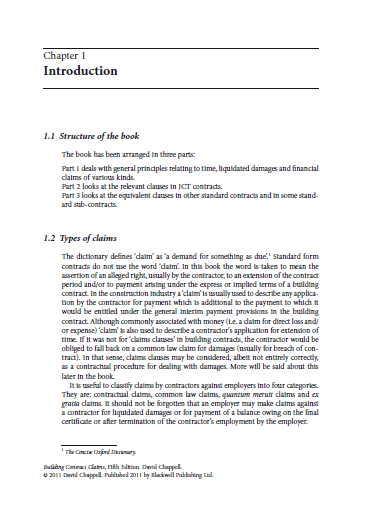
\includegraphics[width=0.45\textwidth]{./chapters/chapter23}
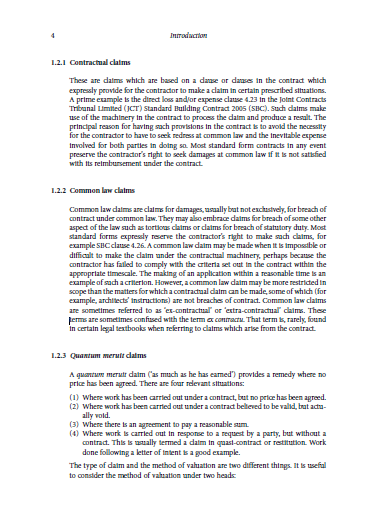
\includegraphics[width=0.45\textwidth]{./chapters/chapter23a}}
\end{figure}

\subsection{Subsections}
The same style is applied to the subsectioning commands up to the subsubsection which is not numbered but just uses an italic font. The subsubsection is also indented into the margin. Since the book is about construction claims it follows a style found in legal and construction documents, where all paragraphs are indented with respect to the section headings.
\lipsum[1-2]
\section{Even pages}
\lipsum[2]
\subsection{Setting different margins}
\lipsum[1]
\subsubsection{Setting Subsubsections}
\lipsum[1]
\paragraph{Paragraph level. } \lipsum*[3]\par

\lipsum[1]
\subparagraph{sub-paragraph level. } \lipsum*[3]\par


\restoregeometry
%%%%%%%%%%%%%%%%%%%%%%%%%%%%%%%%%%%%%%%%%%%
%%%%%%  STYLE 24
%%%%%%%%%%%%%%%%%%%%%%%%%%%%%%%%%%%%%%%%%%%
\clearpage
\cxset{
 name=Chapter,
 numbering=arabic,
 number font-size=\Large,
 number font-family=\sffamily,
 number font-weight=\normalfont,
 number before={},
 number after={\space},
 number position=rightname,
 chapter font-family=\sffamily,
 chapter font-weight=\normalfont,
 chapter font-size=\Large,
 number after={},
 number dot=,
 chapter before={},
 chapter after={\par\thinrule\vskip12pt},
 chapter color={black!90},
 number color=\color{black!90},
 title beforeskip={},
 title afterskip={\vspace{30pt}},
 title before=,
 title after={\par},
 title font-family=\sffamily,
 title font-color=\color{black!80},
 title font-weight=\bfseries,
 title font-size=\LARGE,
 title afterskip=\par\vspace*{3cm}\thinrule\par\bigskip\bigskip}
\chapter{Introduction to style twenty four}

\def\objectives@{
\begin{tcolorbox}[width=\linewidth,boxsep=10pt,right=10pt]
\textbf{Learning Objectives}}
\def\stopobjectives@{\end{tcolorbox}}
\newenvironment{objectives}{\bigskip\objectives@}{\stopobjectives@\bigskip}

\begin{objectives}
\par
\lipsum[1]
\bigskip\bigskip
\end{objectives}

This design is ideal for scholarly books or notes. It has a nice clean design with a shaded block for the learning objectives.
\medskip
\begin{figure}[ht]
\centering
\fbox{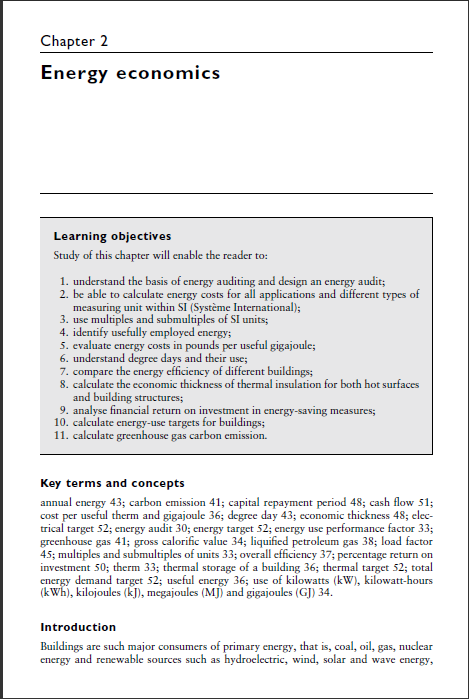
\includegraphics[width=0.6\textwidth]{./chapters/chapter24}}
\end{figure}
\lipsum[2-3]


%%%%%%%%%%%%%%%%%%%%%%%%%%%%%%%%%%%%%%%%%%%
%%%%%%  STYLE 25
%%%%%%%%%%%%%%%%%%%%%%%%%%%%%%%%%%%%%%%%%%%

\cxset{author/.store in=\author@cx}

\cxset{style25/.style={
 name={CHAPTER},
 numbering=arabic,
 number font-size=\huge,
 number font-family=\sffamily,
 number font-weight=\normalfont,
 number before={},
 number position=rightname,
 chapter font-family=\sffamily,
 chapter font-weight=\normalfont,
 chapter font-size=\huge,
 number after={},
 chapter before={\thinrule\par\vspace{3pt}\hfill},
 chapter after={\hfill\hfill\par\vspace{-10pt}\thinrule\par\leavevmode},
 chapter color={black!90},
 number color=\color{black!90},
 title beforeskip={\centering},
 title afterskip={\vspace{20pt}\author@cx},
 title before=\leavevmode,
 title after={\par\vspace{-20pt}\thinrule\par},
 title font-family=\sffamily,
 title font-color=\color{black!80},
 title font-weight=\bfseries,
 title font-size=\huge}}

\cxset{author=\centering\bfseries\upshape\large Yiannis Lazarides and Athena Lazarides\par\vspace{30pt}}

\setstyle{25}
\chapter{INTRODUCTION TO STYLE 25}

The interesting part of this style is that it uses roman numerals to display the counter that is in a different font than that used for the chapter name.
\medskip
\begin{figure}[ht]
\centering
\fbox{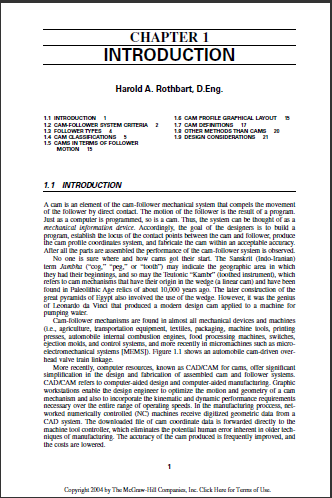
\includegraphics[width=0.5\textwidth]{chapter25}}
\end{figure}
\lipsum[1-2]

%\end{document}
%%%%%%%%%%%%%%%%%%%%%%%%%%%%%%%%%%%%%%%%%%%
%%%%%%  STYLE 26
%%%%%%%%%%%%%%%%%%%%%%%%%%%%%%%%%%%%%%%%%%%

\cxset{
 name={},
 numbering=arabic,
 number font-size=\huge,
 number font-family=\sffamily,
 number font-weight=\bfseries,
 number before={},
 number position=leftname,
 chapter font-family=\sffamily,
 chapter font-weight=\normalfont,
 chapter font-size=\small,
 number after={},
 chapter before={},
 chapter after={\par\vskip12pt},
 chapter color={black!90},
 number color=\color{black!90},
 title beforeskip={},
 title afterskip={\vspace{30pt}},
 title before=,
 title after={\par},
 title font-family=\sffamily,
 title font-color=\color{black!80},
 title font-weight=\bfseries,
 title font-size=\LARGE}
\chapter{Introduction to style twenty five Dr. Yiannis Lazarides and Athena Lazarides}

The interesting part of this style is that it uses roman numerals to display the counter that is in a different font than that used for the chapter name.
\medskip
\begin{figure}[ht]
\centering
\fbox{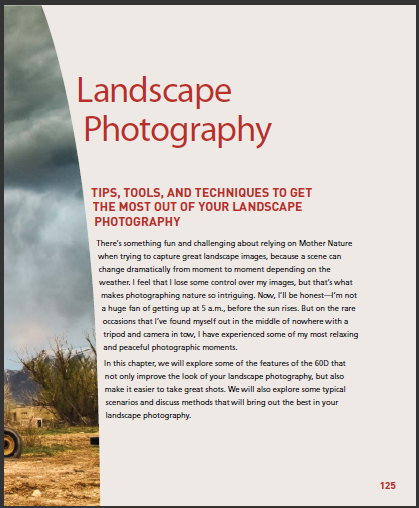
\includegraphics[width=0.6\textwidth]{./chapters/chapter26}}
\end{figure}
\lipsum[2-3]


\newgeometry{top=2cm,bottom=2cm}
%%%%%%%%%%%%%%%%%%%%%%%%%%%%%%%%%%%%%%%%%%%
%%%%%%  STYLE 27
%%%%%%%%%%%%%%%%%%%%%%%%%%%%%%%%%%%%%%%%%%%

\cxset{
 name={},
 numbering=arabic,
 number font-size=\HUGE,
 number font-family=\sffamily,
 number font-weight=\bfseries,
 number before={},
 number dot=,
 number position=leftname,
 chapter font-family=\sffamily,
 chapter font-weight=\normalfont,
 chapter font-size=\small,
 number after={},
 chapter before={\vspace*{50pt}},
 chapter after={\par\vskip12pt},
 chapter color={black!90},
 number color=\color{black!90},
 title beforeskip={},
 title afterskip={\vspace{30pt}},
 title before=,
 title after={\par},
 title font-family=\sffamily,
 title font-color=\color{black!80},
 title font-weight=\bfseries,
 title font-size=\huge}
\chapter{Introduction to style twenty seven Dr. Yiannis Lazarides and Athena Lazarides}
\lipsum[3]

\medskip
\begin{figure}[ht]
\centering
\fbox{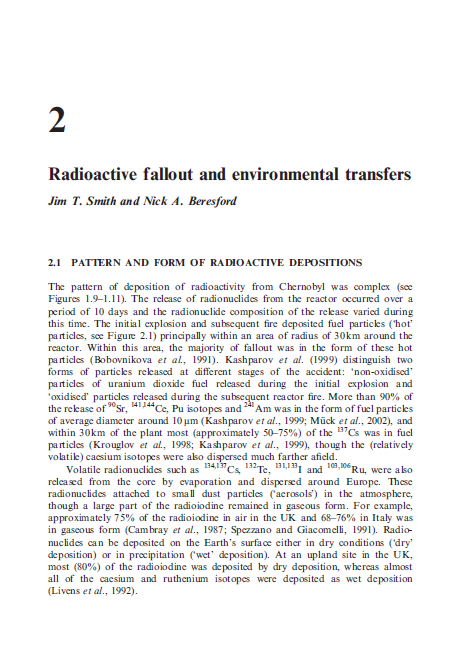
\includegraphics[width=0.5\textwidth]{./chapters/chapter27}}
\end{figure}
\lipsum[2-3]


%%%%%%%%%%%%%%%%%%%%%%%%%%%%%%%%%%%%%%%%%%%
%%%%%%  STYLE 28
%%%%%%%%%%%%%%%%%%%%%%%%%%%%%%%%%%%%%%%%%%%

\cxset{
 name={},
 numbering=arabic,
 number font-size=\HUGE,
 number font-family=\sffamily,
 number font-weight=\bfseries,
 number before={},
 number position=leftname,
 chapter font-family=\sffamily,
 chapter font-weight=\normalfont,
 chapter font-size=\small,
 number after={},
 chapter before={},
 chapter after={\hspace*{20pt}},
 chapter color={black!90},
 number color=\color{black!90},
 title beforeskip={},
 title afterskip={\vspace{70pt}},
 title before=,
 title after={\par},
 title font-family=\itshape,
 title font-color=\color{black!80},
 title font-weight=\itshape,
 title font-size=\LARGE}
\chapter{Introduction to Style Twenty Eight}

The interesting part of this style is that it uses roman numerals to display the counter that is in a different font than that used for the chapter name.
\medskip
\begin{figure}[ht]
\centering

\includegraphics[width=0.6\textwidth]{./chapters/chapter28}
\end{figure}
\lipsum[2]

%%%%%%%%%%%%%%%%%%%%%%%%%%%%%%%%%%%%%%%%%%%
%%%%%%  STYLE 29
%%%%%%%%%%%%%%%%%%%%%%%%%%%%%%%%%%%%%%%%%%%
 \cxset{style29/.style={
 name={},
 numbering=arabic,
 number font-size=\normalsize,
 number font-family=\sffamily,
 number font-weight=\bfseries,
 number before={\vspace*{50pt}},
 number position=leftname,
 number after=\vskip-7.5pt,
 chapter font-family=\sffamily,
 chapter font-weight=,
 chapter font-size=\small,
 chapter before={\vskip2.5pt},
 chapter after={\thinrule\par},
 chapter color={black!90},
 number color=\color{black!90},
 title beforeskip={},
 title afterskip={\bigskip},
 title before=,
 title after={\par},
 title font-family=\rmfamily,
 title font-color=\color{black!80},
 title font-weight=\bfseries,
 title font-size=\huge},
 section indent=0pt,
 section font-family=\rmfamily,
 section font-shape=\upshape}
\cxset{style29}

\chapter{Introduction to Style Twenty Nine}
\bigskip\bigskip

\textit{Lambert Schoemacher}
\bigskip\bigskip\bigskip\bigskip

\section{Introduction}
The interesting part of this style is that it uses roman numerals to display the counter that is in a different font than that used for the chapter name.
\medskip

\begin{figure}[ht]
\centering
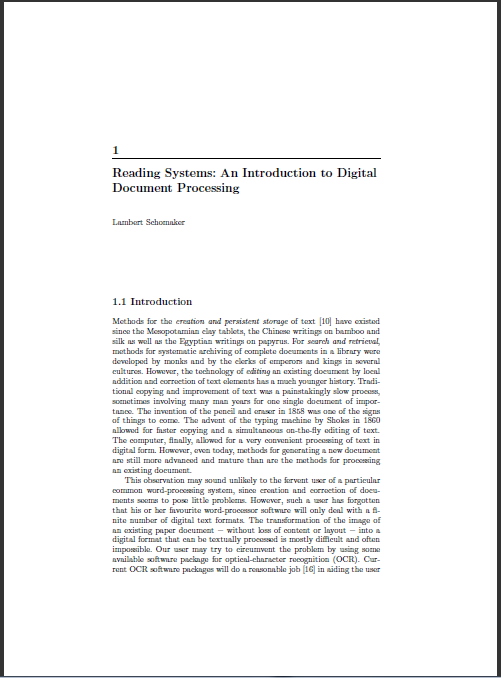
\includegraphics[width=0.6\textwidth]{./chapters/chapter29}
\end{figure}
\lipsum[3]

%%%%%%%%%%%%%%%%%%%%%%%%%%%%%%%%%%%%%%%%%%%
%%%%%%  STYLE 30
%%%%%%%%%%%%%%%%%%%%%%%%%%%%%%%%%%%%%%%%%%%

\cxset{style30/.style={
 name={},
 numbering=arabic,
 number font-size=\HUGE,
 number font-family=\sffamily,
 number font-weight=\bfseries,
 number before={\rule{\textwidth}{5pt}\par\vspace*{12pt}\hspace*{20pt}\minipage{1cm}\vspace*{8pt}},
 number after=\endminipage\hspace{1em},
 number position=leftname,
 chapter font-family=\sffamily,
 chapter font-weight=\normalfont,
 chapter font-size=\small,
 chapter before={},
 chapter after={\hspace*{20pt}},
 chapter color={black!90},
 number color=\color{black!90},
 title beforeskip={},
 title afterskip={\vspace{30pt}},
 title before=\minipage[t]{10cm},
 title after={\endminipage\par},
 title font-family=\sffamily,
 title font-color=\color{black!80},
 title font-weight=\normalfont\sffamily,
 title font-size=\Huge}}

\cxset{style30}
\chapter{Introduction to Style Thirty\\ with a Somehow Long Title \\to Illustrate the Example}

Since we do not know how long a chapter title can end up, it is best to
typeset this using two minipages or parboxes. The number is pushed down slightly although it can look as good with both the number and the text fully aligned on top.
\medskip
\begin{figure}[ht]
\centering
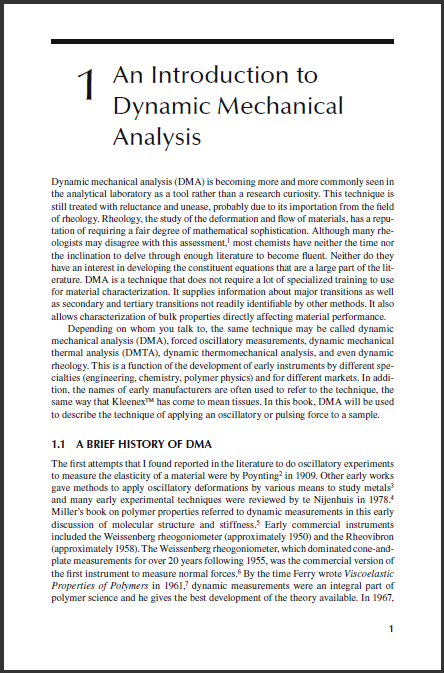
\includegraphics[width=0.6\textwidth]{./chapters/chapter30}
\end{figure}



%%%%%%%%%%%%%%%%%%%%%%%%%%%%%%%%%%%%%%%%%%%
%%%%%%  STYLE 31
%%%%%%%%%%%%%%%%%%%%%%%%%%%%%%%%%%%%%%%%%%%

\cxset{style31/.style={
 name={},
 numbering=arabic,
 number font-size=\HUGE,
 number font-family=\sffamily,
 number font-weight=\bfseries,
 number before=,
 number after={},
 number position=leftname,
 chapter font-family=\sffamily,
 chapter font-weight=\normalfont,
 chapter font-size=\small,
 chapter before={},
 chapter after={\vskip2.5pt{\color{gray}\rule{3cm}{5pt}\rule[3.5pt]{\dimexpr\textwidth-3cm\relax}{0.4pt}}\par},
 chapter color={gray},
 number color=\color{gray},
 title beforeskip={},
 title afterskip={\vspace{30pt}},
 title before=,
 title after={\par{\color{gray}\rule[6pt]{3cm}{0.4pt}}\par},
 title font-family=\itshape,
 title font-color=\color{black},
 title font-weight=\itshape,
 title font-size=\LARGE}}

\cxset{style31}
\chapter{The Evolution of Organizations\\ and the Environment}

This is an unusual design by all counts. I did soften the rules a bit to make them a bit less conspicuous.
\medskip
\begin{figure}[ht]
\centering
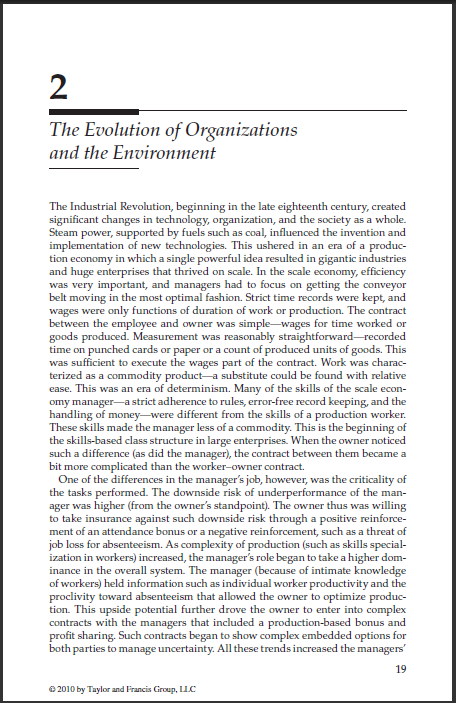
\includegraphics[width=0.6\textwidth]{./chapters/chapter31}
\end{figure}

\lipsum[1-2]

%%%%%%%%%%%%%%%%%%%%%%%%%%%%%%%%%%%%%%%%%%%
%%%%%%  STYLE 32
%%%%%%%%%%%%%%%%%%%%%%%%%%%%%%%%%%%%%%%%%%%

\newgeometry{left=5cm,right=2cm,bottom=2cm}
\cxset{style32/.style={
 name={},
 numbering=arabic,
 number font-size=\HUGE,
 number font-family=\sffamily,
 number font-weight=\bfseries,
 number before={\hspace*{-10pt}},
 number position=leftname,
 chapter font-family=\sffamily,
 chapter font-weight=\normalfont,
 chapter font-size=\small,
 number after={},
 chapter before={\vspace*{50pt}\par\hspace*{-60pt}},
 chapter after={\hspace*{20pt}},
 chapter color={black!90},
 number color=\color{black!90},
 title beforeskip={},
 title afterskip={\vspace{70pt}},
 title before=,
 title after={\par},
 title font-family=\itshape,
 title font-color=\color{black!80},
 title font-weight=\bfseries,
 title font-shape=\itshape,
 title font-size=\Huge,
 blank page text= \epigraph{TeX needs patience}{Dr Y Lazarides},
}}
\cxset{style32}
\chapter{Introduction to Style Thirty Two}

This style has a modern look to it. Its main characteristic is the large chapter number and the fact that it is drawn into the margin. A common style for computer books.
\medskip
\begin{figure}[ht]
\centering
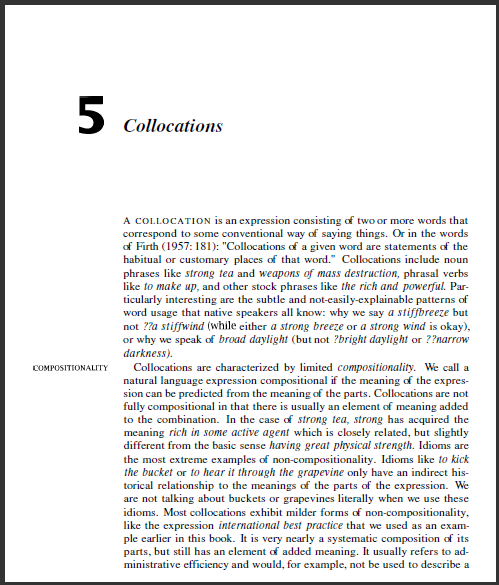
\includegraphics[width=0.6\textwidth]{./chapters/chapter32}
\end{figure}
The example is from Python NLP book.

%%%%%%%%%%%%%%%%%%%%%%%%%%%%%%%%%%%%%%%%%%%
%%%%%%  STYLE 33
%%%%%%%%%%%%%%%%%%%%%%%%%%%%%%%%%%%%%%%%%%%
\restoregeometry
\cxset{style33/.style={
 name=CHAPTER,
 numbering=arabic,
 number font-size=\LARGE,
 number font-family=\rmfamily,
 number font-weight=\normalfont,
 number before={\par\hfill},
 number after={\hfill\hfill\par},
 number position=leftname,
 name=,
 chapter font-family=\sffamily,
 chapter font-weight=\normalfont,
 chapter font-size=\small,
 chapter before={\vskip10pt},
 chapter after={\vskip10pt\par},
 chapter color={black!90},
 number color=\color{black!90},
 title beforeskip={},
 title afterskip={\vspace{50pt}},
 title before=\hfill,
 title after={\hfill\hfill\par},
 title font-family=\normalfont,
 title font-color=\color{black!80},
 title font-weight=\normalfont,
 title font-shape=\upshape,
 title font-size=\LARGE,
 section numbering=none,
 section font-size=\Large,
 section align=\centering}}

\cxset{style33}
\chapter{Introduction to Style Thirty Three}

The interesting part of this style is that it uses roman numerals to display the counter that is in a different font than that used for the chapter name.
\medskip
\begin{figure}[ht]
\centering
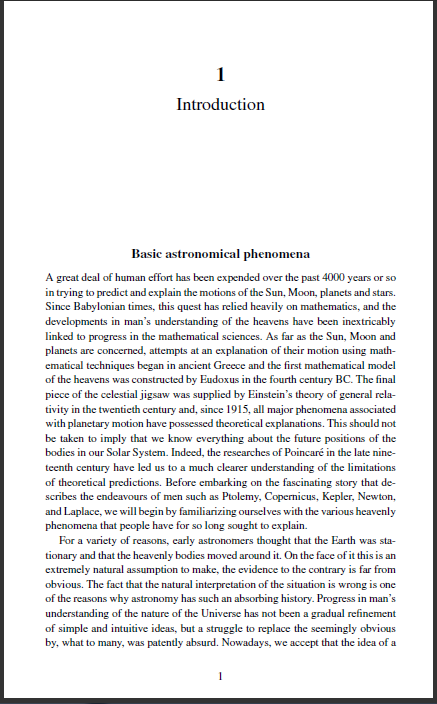
\includegraphics[width=0.6\textwidth]{./chapters/chapter33}
\end{figure}





%%%%%%%%%%%%%%%%%%%%%%%%%%%%%%%%%%%%%%%%%%%
%%%%%%  STYLE 34
%%%%%%%%%%%%%%%%%%%%%%%%%%%%%%%%%%%%%%%%%%%

\cxset{
 name=CHAPTER,
 numbering=Roman,
 number font-size=\small,
 number font-family=\rmfamily,
 number font-weight=\normalfont,
 number before={},
 number position=rightname,
 chapter font-family=\sffamily,
 chapter font-weight=\normalfont,
 chapter font-size=\small,
 number after={},
 chapter before={},
 chapter after={\par},
 chapter color={black!90},
 number color=\color{black!90},
 title beforeskip={},
 title afterskip={\vspace{50pt}},
 title before=,
 title after={\par},
 title font-family=\normalfont,
 title font-color=\color{black!80},
 title font-weight=\normalfont,
 title font-size=\LARGE}

\section{Basic astronomical phenomena}

The interesting part of this style is that it uses roman numerals to display the counter that is in a different font than that used for the chapter name.
\medskip
\begin{figure}[ht]
\centering
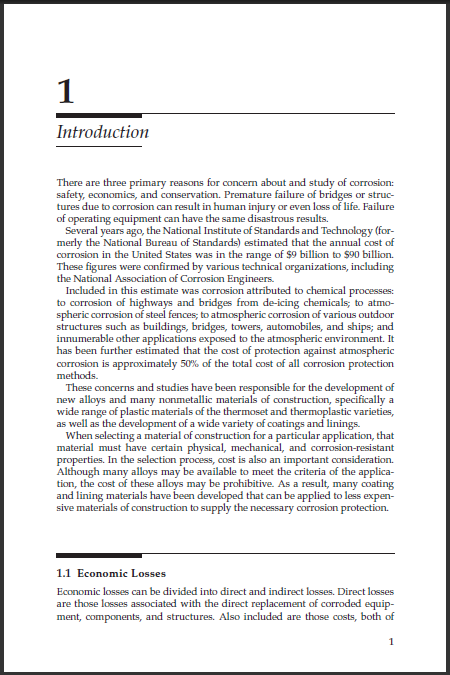
\includegraphics[width=0.6\textwidth]{./chapters/chapter34}
\end{figure}


%%%%%%%%%%%%%%%%%%%%%%%%%%%%%%%%%%%%%%%%%%%
%%%%%%  STYLE 35
%%%%%%%%%%%%%%%%%%%%%%%%%%%%%%%%%%%%%%%%%%%

\cxset{%
 name=CHAPTER,
 numbering=Roman,
 number font-size=\small,
 number font-family=\rmfamily,
 number font-weight=\normalfont,
 number before={},
 number position=rightname,
 chapter font-family=\sffamily,
 chapter font-weight=\normalfont,
 chapter font-size=\small,
 number after={},
 chapter before={},
 chapter after={\par},
 chapter color={black!90},
 number color=\color{black!90},
 title beforeskip={},
 title afterskip={\vspace{50pt}},
 title before=,
 title after={\par},
 title font-family=\normalfont,
 title font-color=\color{black!80},
 title font-weight=\normalfont,
 title font-size=\LARGE}
\chapter{Introduction to Style Thirty Five}

The interesting part of this style is that it uses roman numerals to display the counter that is in a different font than that used for the chapter name.
\medskip

\begin{figure}[ht]
\centering
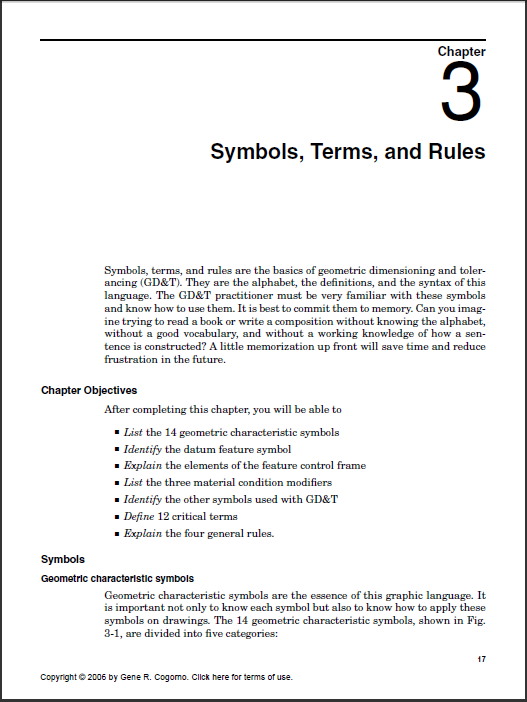
\includegraphics[width=0.6\textwidth]{./chapters/chapter35}
\end{figure}


%%%%%%%%%%%%%%%%%%%%%%%%%%%%%%%%%%%%%%%%%%%
%%%%%%  STYLE 36
%%%%%%%%%%%%%%%%%%%%%%%%%%%%%%%%%%%%%%%%%%%

\cxset{numbering=none}
%% has errors
\cxset{style36/.style={
 name={},
 numbering={none},
 number font-size=\small,
 number font-family=\rmfamily,
 number font-weight=\normalfont,
 number before={},
 number position=rightname,
 chapter font-family=\sffamily,
 chapter font-weight=\normalfont,
 chapter font-size=\small,
 number after={},
 chapter before={},
 chapter after={},
 chapter color={black!90},
 number color=\color{black!90},
 title beforeskip={},
 title before=,
 title after={\vskip-12.5pt\rule{\columnwidth}{3.5pt}\vspace*{50pt}},
 title afterskip={},
 title font-family=\sffamily,
 title font-color=\color{black!80},
 title font-weight=\bfseries,
 title font-size=\Huge}}

\cxset{style36}
\chapter{Introduction to Style Thirty Six}

The interesting part of this style is that it uses roman numerals to display the counter that is in a different font than that used for the chapter name.
\medskip

\begin{figure}[ht]
\centering
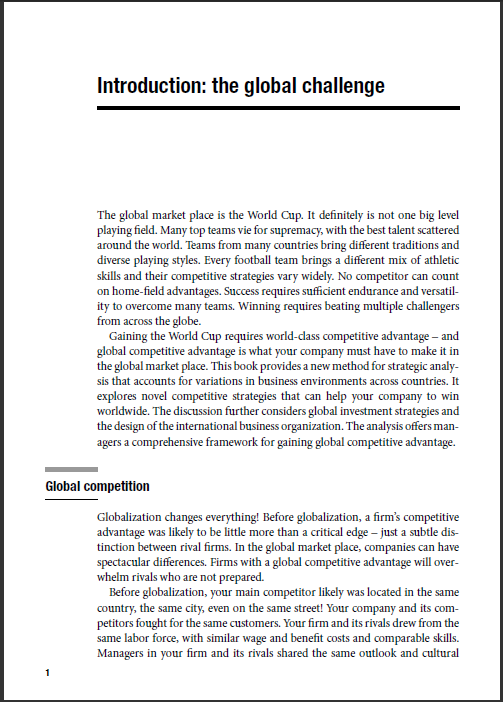
\includegraphics[width=0.6\textwidth]{./chapters/chapter36}
\end{figure}


%%%%%%%%%%%%%%%%%%%%%%%%%%%%%%%%%%%%%%%%%%%
%%%%%%  STYLE 37
%%%%%%%%%%%%%%%%%%%%%%%%%%%%%%%%%%%%%%%%%%%

\cxset{style37/.style={
 name=CHAPTER,
 numbering=Roman,
 number font-size=\small,
 number font-family=\rmfamily,
 number font-weight=\normalfont,
 number before={},
 number position=rightname,
 chapter font-family=\sffamily,
 chapter font-weight=\normalfont,
 chapter font-size=\small,
 chapter spaceout=soul,
 number after={},
 chapter before={},
 chapter after={\par},
 chapter color={black!90},
 number color=\color{black!90},
 title beforeskip={},
 title afterskip={\vspace{50pt}},
 title before=,
 title after={\par},
 title font-family=\normalfont,
 title font-color=\color{black!80},
 title font-weight=\bfseries,
 title font-size=\huge}}

\cxset{style37}
\chapter{Introduction to Style Thirty Seven}

The interesting part of this style is that it uses roman numerals to display the counter that is in a different font than that used for the chapter name.
\medskip

\begin{figure}[ht]
\centering
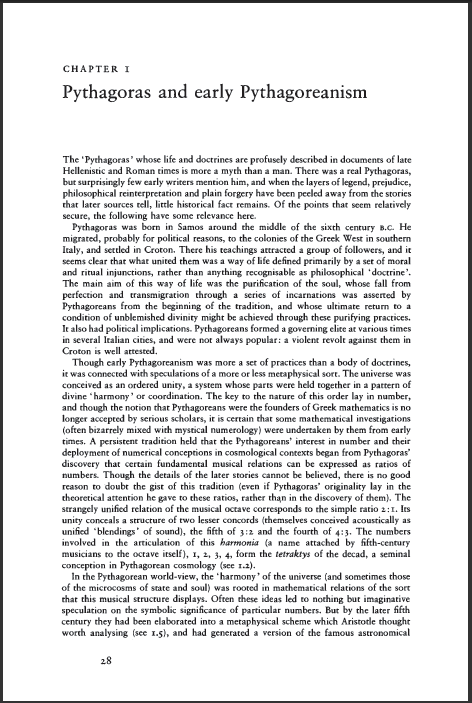
\includegraphics[width=0.6\textwidth]{./chapters/chapter37}
\end{figure}


%%%%%%%%%%%%%%%%%%%%%%%%%%%%%%%%%%%%%%%%%%%
%%%%%%  STYLE 38
%%%%%%%%%%%%%%%%%%%%%%%%%%%%%%%%%%%%%%%%%%%

\cxset{style38/.style={
 name=,
 numbering=arabic,
 number font-size=\huge,
 number font-family=\rmfamily,
 number font-weight=\normalfont,
 number before={\begin{center}},
 number position=leftname,
 chapter font-family=\sffamily,
 chapter font-weight=\normalfont,
 number after={\vspace*{6.5pt}\par},
 chapter before={},
 chapter after={},
 chapter color={black!90},
 number color=\color{black!90},
 title beforeskip={},
 title afterskip={\vspace{50pt}},
 title before=,
 title after={\par\end{center}} ,
 title font-family=\rmfamily,
 title font-color=\color{black!80},
 title font-weight=\normalfont,
 title font-size=\huge,
 chapter font-size=,
}}

\cxset{style38,
       author block=true,
       author block format=\centering}
\chapter{STAGES OF INITIATION IN THE\\ ELEUSINIAN AND\\ SAMOTHRACIAN MYSTERIES\\STYLE 38}

This style uses rules to enclose both the chapter name and number as well as the title, which necessarily needs to be rather short.
\medskip

\begin{figure}[ht]
\centering
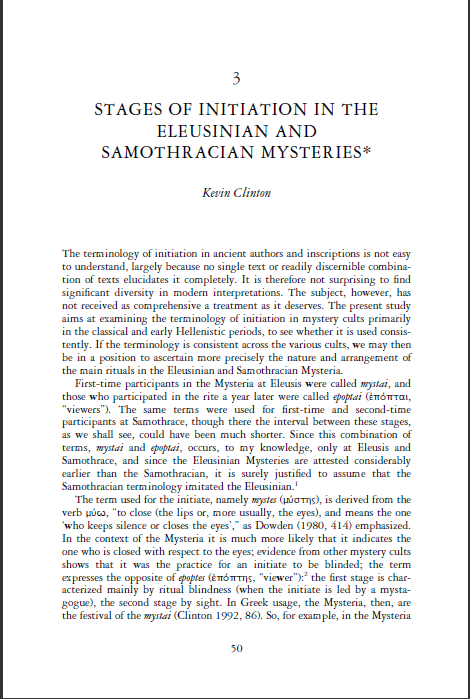
\includegraphics[width=0.6\textwidth]{./chapters/chapter38}
\end{figure}



%%%%%%%%%%%%%%%%%%%%%%%%%%%%%%%%%%%%%%%%%%%
%%%%%%  STYLE 39
%%%%%%%%%%%%%%%%%%%%%%%%%%%%%%%%%%%%%%%%%%%

\cxset{
 name=CHAPTER,
 numbering=arabic,
 number font-size=\LARGE,
 number font-family=\sffamily,
 number font-weight=\bfseries,
 number before={},
 number position=rightname,
 chapter font-family=\sffamily,
 chapter font-weight=\bfseries,
 number after={},
 chapter before={\rule{\textwidth}{2pt}\par},
 chapter after={\vskip0pt\vspace*{-8pt}\rule{\textwidth}{.4pt}\vskip-7pt},
 chapter color={black!90},
 number color=\color{black!90},
 title beforeskip={},
 title afterskip={\vspace{50pt}},
 title before=,
 title after={\par\vskip-16.5pt\rule{\textwidth}{0.4pt}\par} ,
 title font-family=\sffamily,
 title font-color=\color{black!80},
 title font-weight=\bfseries,
 title font-size=\LARGE,
 chapter font-size=\LARGE,
 author block=false}

\chapter{STYLE 39}

This style uses rules to enclose both the chapter name and number as well as the title, which necessarily needs to be rather short.
\medskip

\begin{figure}[ht]
\centering
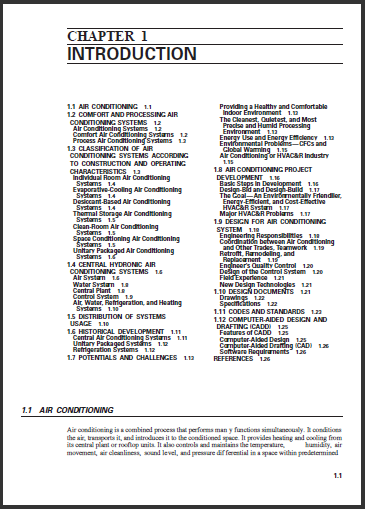
\includegraphics[width=0.6\textwidth]{./chapters/chapter39}
\end{figure}
In the picture it does not look very attractive, but in the actual book it does. My observation is that the rule clearances are a bit tight and if you use this type of layout it is better to experiment until you get them right.

\begin{tcblisting}{}
\@makechapterhead[
 name=CHAPTER,
 numbering=arabic,
 number font-size=\LARGE,
 number font-family=\sffamily,
 number font-weight=\bfseries,
 number before={},
 number position=rightname,
 chapter font-family=\sffamily,
 chapter font-weight=\bfseries,
 number after={},
 chapter before={\rule{\textwidth}{2pt}\par},
 chapter after={\vskip0pt\vspace*{-8pt}\rule{\textwidth}{.4pt}\vskip-7pt},
 chapter color={black!90},
 number color=\color{black!90},
 title beforeskip={},
 title afterskip={\vspace{50pt}},
 title before=,
 title after={\par\vskip-19pt\rule{\textwidth}{0.4pt}\par} ,
 title font-family=\sffamily,
 title font-color=\color{black!80},
 title font-weight=\bfseries,
 title font-size=\LARGE,
 chapter font-size=\LARGE]{INTRODUCTION}
\end{tcblisting}


%%%%%%%%%%%%%%%%%%%%%%%%%%%%%%%%%%%%%%%%%%%
%%%%%%  STYLE 40
%%%%%%%%%%%%%%%%%%%%%%%%%%%%%%%%%%%%%%%%%%%

\cxset{
 name=,
 numbering=arabic,
 number font-size=\LARGE,
 number font-family=\sffamily,
 number font-weight=\bfseries,
 number before={},
 number position=rightname,
 chapter font-family=\sffamily,
 chapter font-weight=\bfseries,
 chapter before=\hfill,
 number after=,
 chapter after=\hfill\hfill\vskip0pt ,
 chapter color={black!90},
 number color=\color{black!90},
 title beforeskip=,
 title before=\begin{center},
 title after=\end{center},
 title font-family=\sffamily,
 title font-color=\color{black!80},
 title font-weight=\bfseries,
 title font-size=\LARGE,
 chapter font-size=\LARGE,
 author block=true,
 author block format=\normalfont\Large\centering,
 author names=Karin Wahl-Jorgensen and Thomas Hanitzch}


\chapter{Introduction:\\ On Why and How to Use\\ Chapter Style Forty}

A simple design for sombre multi-author books. This is now common in many publications such as proceedings, conferences and the like. They are actually mostly collections of articles, but formatted as books.

\begin{figure}[ht]
\centering

\includegraphics[width=0.6\textwidth]{./chapters/chapter40}
\end{figure}

One issue with such designs is how to make it easy for the user to add the author block. There are two pathways, the one is to use \cs{cxset} and the other is to make a special command for it.

\newcommand\addauthors[1]{
   \cxset{author names=#1}
}


%\cxset{author names=Yiannis Lazarides}

%%%%%%%%%%%%%%%%%%%%%%%%%%%%%%%%%%%%%%%%%%%
%%%%%%  STYLE 41
%%%%%%%%%%%%%%%%%%%%%%%%%%%%%%%%%%%%%%%%%%%

\cxset{chapter author/.store in=\chapterauthor@cx}
\cxset{style41/.style={
 color=purple,
 name=CHAPTER,
 numbering=WORDS,
 number font-size=\large,
 number font-family=\rmfamily,
 number font-weight=\normalfont,
 number before={},
 number position=rightname,
 chapter font-family=\rmfamily,
 chapter font-weight=\normalfont,
 chapter before=\hfill,
 chapter spaceout=none,
 number after=,
 chapter after=\hfill\hfill\vskip0pt,
 chapter color={black!90},
 number color=\color{black!90},
 title beforeskip=,
 title before=\begin{center},
 title after=\par\normalfont\floweroneleft\floweroneright\par\end{center},
 title spaceout=none, % does not work, needs a work around
 title font-family=\rmfamily,
 title font-color=\color{black!80},
 title font-weight=\normalfont,
 title font-size=\LARGE,
 chapter font-size=\large,
 section numbering=none,
 section indent=0pt,
 section align=\centering,
 section font-shape=\upshape,
 section font-weight=\normalfont,
 section font-size=\large,
 section spaceout=soul,
}}

\cxset{style41,
       chapter author=Yiannis Lazarides,
       epigraph width=0.85\textwidth,
       epigraph text align=left,
       epigraph source align=right,
       epigraph rule width=0pt,
       epigraph afterskip=50pt,
       author block format=\normalfont\itshape\Large\centering,
}

\addauthors{Dr Yiannis Lazarides}
\chapter{{INTRODUCTION TO}\\ {CHAPTER STYLE FORTY ONE}}
\label{ch:41}
\epigraph{The existence of an area of free land, its continuous recession, and the advance of American
settlement westward explain American development.}{Frederick Jackson Turner, \textit{The Significance of the Frontier in American\\ History,} Columbian Exploration, Chicago, July 12, 1893}

A classical style chapter style with finely spaced out letters. A number of books spell out the chapter numbers. In general I find this as a good idea as sometimes the numbers don't blend in very well with the design.

\begin{figure}[ht]
\centering
\fbox{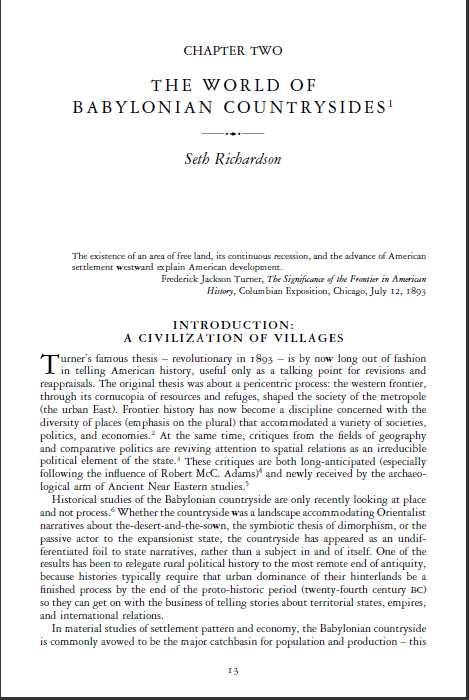
\includegraphics[width=0.5\textwidth]{./chapters/chapter41}}
\end{figure}

This book has different chapters written by different authors and the author's name appear below an ornament. Don't dismiss ornaments as old fashioned as a lot of modern books still use them.

\begin{lstlisting}
\cxset{style41,
         chapter author=Yiannis Lazarides}
\end{lstlisting}

The ornaments I used was from the \texttt{fourier-orns} package. Here is a MWE if you want to experiment with various designs.


\begin{lstlisting}
\documentclass{article}
\usepackage{fourier-orns}
\begin{document}
\Huge
\textxswup\textxswdown
\decoone\decotwo
\decothreeleft\decothreeright
\decofourleft\decofourright
\floweroneleft\floweroneright
\end{document}
\end{lstlisting}

\section{THINGS THAT ARE NOT AUTOMATED}

If you need the title to be spaced out using the soul package and you have a line break, the package will issue the error `reconstruction failed'. In this case it is better to include the spaceout commands in the title.


\begin{verbatim}
\chapter{\so{INTRODUCTION TO}\\ \so{CHAPTER STYLE FORTY ONE}}
\end{verbatim}


%% STYLE 42
\cxset{style42/.style={
 name=,
 numbering=padzeroes,
 number font-size=\huge,
 number before={},
 number position=leftname,
 chapter before=\vspace*{10pt},
 number after=\hfill\hfill,
 chapter after=\hfill\hfill\vskip20pt ,
 number color=\color{gray},
 title font-family=\sffamily,
 title font-color=\color{black!80},
 title font-weight=,
 title font-size=\LARGE,
 title before=,
 title after=,
 chapter author,
 chapter font-size=\huge,
 section numbering=none,
 epigraph width=0.85\textwidth,
 epigraph text align=left,
 epigraph source align=right,
 epigraph rule width=0pt,
 epigraph afterskip=30pt,
}}

%headings and section still to do
\cxset{style42}
\chapter{Introduction to Style Forty Two}

\epigraph{Tell me, O Muse, of that ingenious hero who trawled far and wide after he had
sacked the famous town of Troy. Many cities did he visit, and many were the nations with whose manners
and customs he was acquainted; moreover he suffered much by sea while trying to save his own life and bring
his men safely home \ldots }{Homer the \textit{Odyssey}}

Style 42 is shown in the following figure:

\begin{figure}[ht]
\centering
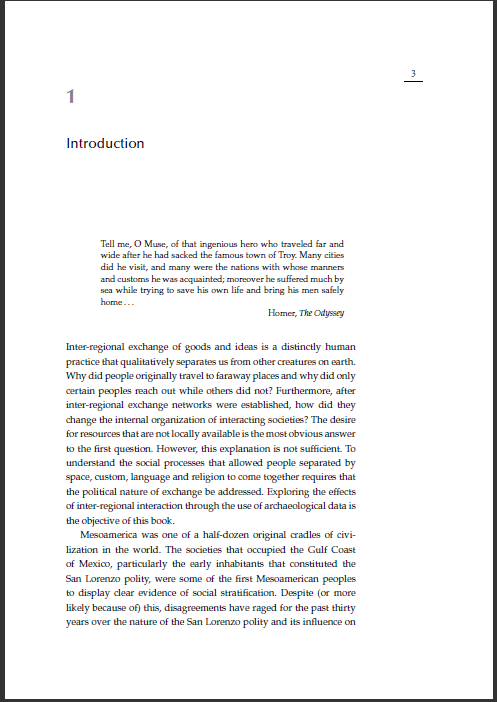
\includegraphics[width=0.6\textwidth]{./chapters/chapter42}
\end{figure}
The distinguishing characteristics of this chapter are that it has an epigraph and is composed of very simple stylistic elements. The epigraph is placed quite a bit lower than the chapter title. The heading style is just the page number and underlined.

%% Chapter 43 Style 43

\cxset{
 name=CHAPTER,
 numbering=arabic,
 number font-size=\Large,
 number before={},
 number position=rightname,
 chapter color={black!80},
 chapter font-size=\Large,
 chapter before=\par\hfill\hfill,
 number after=,
 chapter after=\vskip20pt ,
 number color=\color{black!80},
 title font-family=,
 title font-color=\color{black!95},
 title font-weight=\itshape,
 title font-size=\LARGE,
 title font-shape=\itshape,
 title spaceout=none,
 title beforeskip=\hfill,
 epigraph width=0.95\textwidth,
 epigraph font-size=\normalfont,
 header style=empty,
 blank page text=THIS PAGE LEFT INTENTIONALLY BLANK,
 author block=false}



\cxset{headings ruled-01}
\cxset{chaptermark name=,
          chaptermark after number=,
          header bottom rule=false,
          header style=empty}

\chapter{Introduction to Style 43}

\epigraph{The Jebel Druse is a country of great feudal chiefs, whose efforts are
directed to preserving the powers by which they live.What we call
progress means in their eyes the loss of their privileges and later on
perhaps the partition of their lands.With regard to the inhabitants,
who are ignorant or unmindful of any better fate, they are deeply rooted
in their serfdom and are as conservative as their masters. They have no
aspirations for a system of greater social justice nor [sic] for a better
communal life.}{---Testimony to the League of Nations Permanent Mandates\\
Commission investigating the Syrian Revolt, Geneva, 1926}

\epigraph{Syrians, remember your forefathers, your history, your heroes, your
martyrs, and your national honor. Remember that the hand of God is
with us and that the will of the people is the will of God. Remember
that civilized nations that are united cannot be destroyed.

The imperialists have stolen what is yours. They have laid hands on
the very sources of your wealth and raised barriers and divided your
indivisible homeland. They have separated the nation into religious
sects and states. They have strangled freedom of religion, thought,
conscience, speech, and action.We are no longer even allowed to move
about freely in our own country.

To arms! Let us realize our national aspirations and sacred hopes.

To arms! Confirm the supremacy of the people and the freedom of
the nation.

To arms! Let us free our country from bondage.}{---Excerpt from a rebel manifesto signed\\ by Sultan
al-Atrash and issued on 23 August 1925}

\lettrine{T}his style is reminiscent of the stylistic elements found in Tufte's books with the chapter title set in italics.
\begin{figure}[ht]
\centering
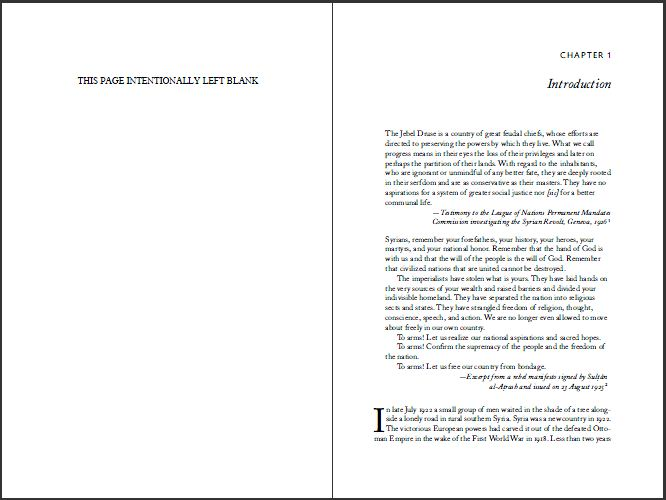
\includegraphics[width=\textwidth]{chapter43.jpg}\par
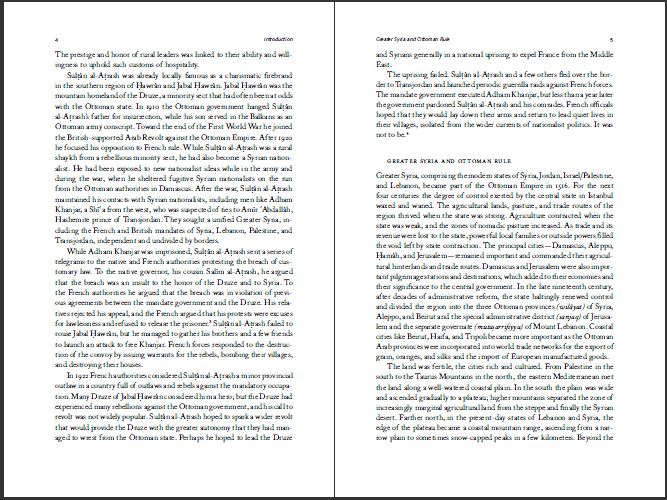
\includegraphics[width=\textwidth]{chapter43a}
\end{figure}
I saw this style in the \textit{The Great Syrian Revolution and the Rise of Arab Nationalism} by Michael Provence, published by the University of Texas at Austin (2005). Notably the best part of the first page is taken by epigraphs, but as you can see from the image, the ugly ``This Page intentionally left blank'' is all over the place, perhaps they could have been mover over? The chapter opens on an even page and bear no headers or footers. The large dropcap at the start of the chapter text balances the ragged left elements of the chapter block.
\lipsum


%% Style 45


\cxset{
 name=,
 numbering=none,
 number font-size=,
 number before=,
 number after=,
 number position=rightname,
 chapter color=black,
 chapter font-size=,
 chapter before=\thinrule,
 chapter after=\vskip20pt ,
 number color=\color{black!80},
 title font-family=\rmfamily,
 title font-color=\color{black!80},
 title font-weight=,
 title font-size=\huge,
 title font-shape=\upshape,
 title beforeskip=,
 title after=\par\vspace*{20pt},
 title afterskip=\vspace*{20pt},
 header style=empty,
 author block format=\normalfont\upshape\LARGE,
 author block=true,
 section align=\raggedright,
 section indent=0pt,
 section font-weight=\bfseries,
 section font-size=\LARGE}

\addauthors{D.T.Potts}
\chapter{A Short Introduction\\ to Style Forty Five\\ including the addition\\of an author}

\section{Introduction}
This is an unusual book with a rather unique style. The vertical rule is simple and breaks the monotony of a book that is heavy on text.
\begin{figure}[ht]
\centering
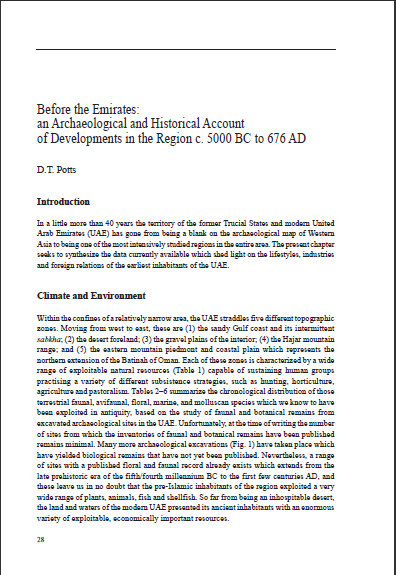
\includegraphics[width=0.6\textwidth]{./chapters/chapter45}
\end{figure}


UNITED ARAB EMIRATES
a new perspective
Edited by
IBRAHIM AL ABED
PETER HELLYERTrident Press Ltd
Layout and design,1997, 2001 Trident Press Ltd,UK.


%% Style 46

\cxset{,
 name=CHAPTER,
 numbering=arabic,
 number font-size=\Large,
 number before={},
 number position=rightname,
 chapter color={black!80},
 chapter font-size=\Large,
 chapter before=\par\hfill\hfill,
 number after=,
 chapter after=\vskip20pt ,
 number color=\color{black!80},
 title font-family=\itshape,
 title font-color=\color{black!80},
 title font-weight=,
 title font-size=\LARGE,
 title beforeskip=\hfill,header style=empty}

\section{Introduction to Style 46}


This is an unusual book with a rather unique style. The vertical rule is simple and breaks the monotony of a book that is heavy on text.
\begin{figure}[ht]
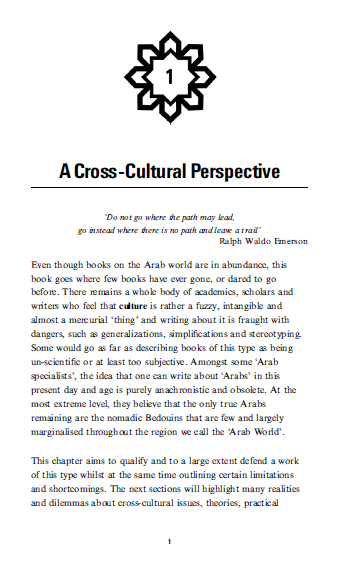
\includegraphics[width=0.45\textwidth]{./chapters/chapter46}
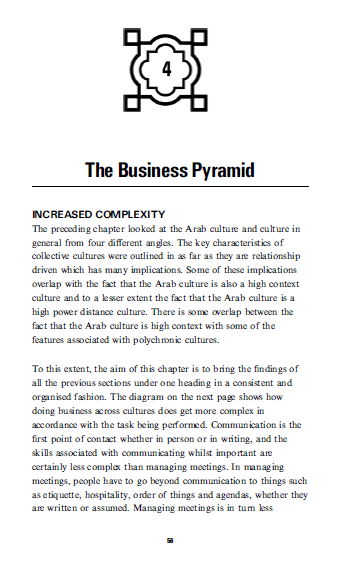
\includegraphics[width=0.45\textwidth]{./chapters/chapter46a}
\end{figure}

Understanding the Arab Culture a cross-cultural guide, second edition, published by How To Content, Dr Jehad Al-Omari,2008.

%% Style 46
\def\anornament{%
\begin{tikzpicture}[decoration={markings,
  mark=between positions 0 and 1 step 8pt
  with { \draw [fill=black] (0,0) circle [radius=1pt];}}]
\path[postaction={decorate}] (0,0) to (15,0);
\end{tikzpicture}}


\cxset{style46/.style={%
 name=CHAPTER,
 numbering=arabic,
 number font-size=\Large,
 number before={},
 number position=rightname,
 chapter color={black!80},
 chapter font-size=\Large,
 chapter before=\par\hfill,
 number after=,
 chapter after=\hfill\hfill\par,
 number color=\color{black!80},
 title font-family=\rmfamily,
 title font-shape=\upshape,
 title font-color=\color{black!80},
 title font-weight=,
 title font-size=\LARGE,
 title before=\par\anornament\par \centering,
 title after= \vskip-10pt\anornament\par\vspace*{10pt},
 title beforeskip=,
 title afterskip=\vspace*{30pt},
 author block format=\large,
 header style=empty}}

\cxset{style46}
\addauthors{Jonathan Taylor}
\chapter{INTRODUCTION TO STYLE\\ FORTY SIX }\label{STYLE:46}

This is an unusual book with a rather unique style. The book is heavy on text and I introduced it to show the possibilities of ornaments with TikZ. The rule is made out of tikz decorations as per an answer on tex.sx.
\begin{figure}[ht]
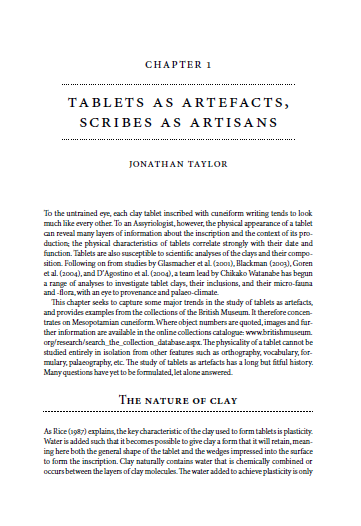
\includegraphics[width=0.48\textwidth]{./chapters/chapter48}\hfill
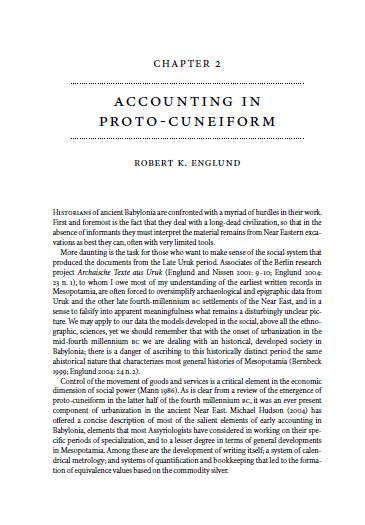
\includegraphics[width=0.48\textwidth]{./chapters/chapter48a}
%\caption{Style 48 from the Oxford Handbook of Cuneiform Culture.}
\end{figure}

This style is very modern and typical of many computer books. The difficulty is in integrating all the page elements to make it work flawlessly.

The Oxford handbook of cuneiform Culture


%% Style 49

\cxset{
 name=CHAPTER,
 numbering=arabic,
 number font-size=\LARGE,
 number font-weight=\bfseries,
 number before=\hfill\vrule height15pt width1.5pt\hspace*{15pt},
 number after=,
 number position=rightname,
 chapter color={black!80},
 chapter font-size=\Large,
 name=,
 chapter before=\vbox to 0pt\bgroup\vskip7.5pt\hbox to \textwidth\bgroup,
 chapter after=\egroup\egroup,
 number color=\color{black!80},
 title font-family=\itshape,
 title font-color=\color{black!80},
 title font-weight=\normalfont,
 title font-size=\Huge,
 title before=\hsize\dimexpr\textwidth-50pt\par\raggedleft,
 title after=\par,
 title beforeskip=,
 header style=empty,
 author block=false}
\chapter{Introduction to Style\\ Forty Nine}

\epigraph{\rightskip50pt Children begin by loving their parents. After a time they judge them. Rarely if ever they forgive them.}{\rightskip35pt---Oscar Wilde, \textit{A woman of No Importance}}

This is an unusual book with a rather unique style. The vertical rule is simple and breaks the monotony of a book that is heavy on text.
\begin{figure}[ht]
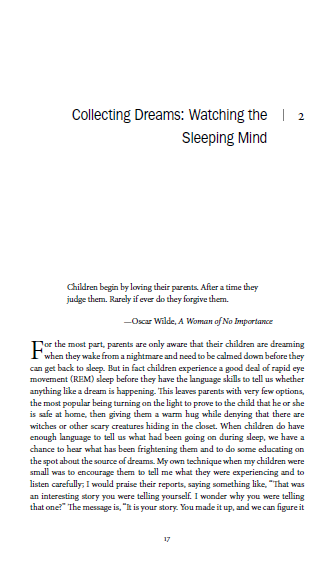
\includegraphics[width=0.48\textwidth]{./chapters/chapter49}\hfill
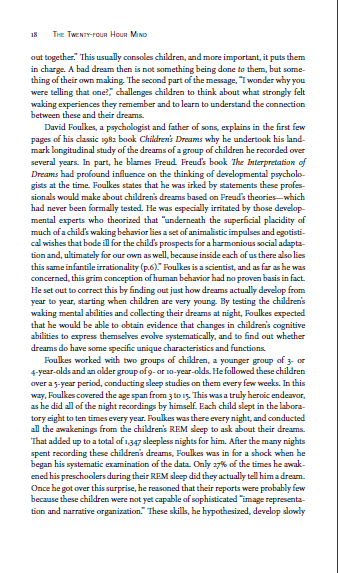
\includegraphics[width=0.48\textwidth]{./chapters/chapter49a}
\caption{Style 48 from the Oxford Handbook of Cuneiform Culture.}
\end{figure}

I battled a bit to set everything and in retrospect chapters like this should have been programmed as specials. However, as soon as they are set, adjustments are easily done.



%% Style 50

\cxset{style50/.style={
 name=,
 numbering=arabic,
 number font-size=\LARGE,
 number font-weight=\bfseries,
 number before={},
 number position=rightname,
 number dot=.,
 chapter color={black!80},
 chapter font-size=,
 chapter before=,
 number after=,
 chapter after=,
 number color=\color{black!80},
 title font-family=\rmfamily,
 title font-color=\color{black!80},
 title before=,
 title after=\par,
 title font-weight=\bfseries,
 title font-size=\LARGE,
 title beforeskip=\space,
 header style=empty,
 author block=true,
 author names=\textsc{James A. Russel and\\[-1.5pt] Jos\'e Miguel Fernandez-Dols },
 author block format=\normalfont\large,
 epigraph width=0.8\textwidth, epigraph align=left}}

\cxset{style50}
\chapter[Chapter Style Fifty]{Introduction to Chapter \\Style Fifty}

\epigraph{\leftskip20pt The human face -- in repose and in movement, at the moment of death as in life, in silence and in speech, when seen or seemed from within, in actuality or as recorded in art or recorded by the camera}{F. Ekman}

This is an unusual book with a rather unique style. The vertical rule is simple and breaks the monotony of a book that is heavy on text.
\begin{figure}[ht]
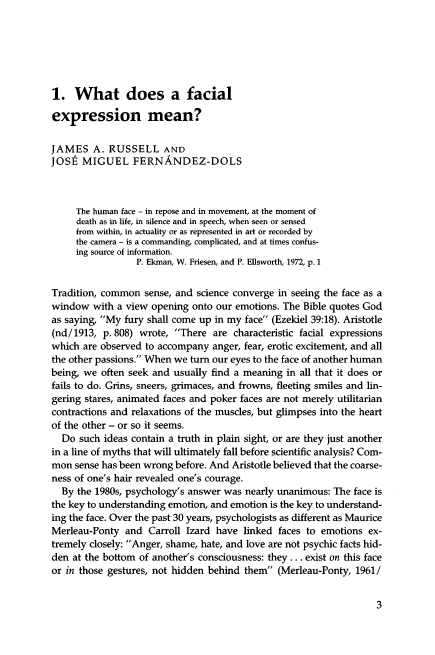
\includegraphics[width=0.48\textwidth]{./chapters/chapter50}\hfill
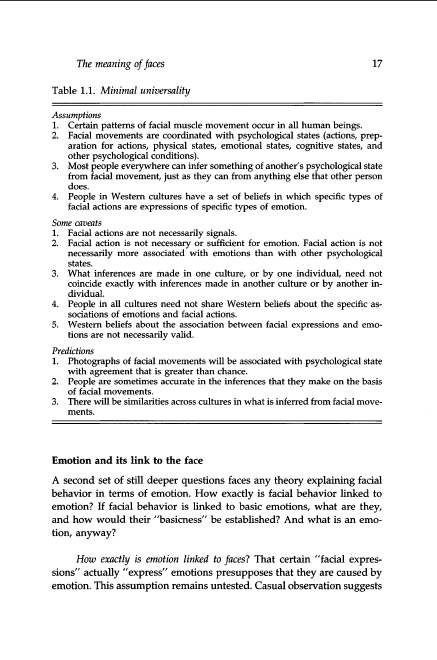
\includegraphics[width=0.48\textwidth]{./chapters/chapter50a}
\caption{Style 50 from the Oxford Handbook of Cuneiform Culture.}
\end{figure}

This style is very modern and typical of many computer books. The difficulty is in integrating all the page elements to make it work flawlessly.

The psychology of facial
expression
Edited by
James A. Russell
University of British Columbia
Jose Miguel Fernandez-Dols
Universidad Autonoma de Madrid, Cambridge University Press.

%% Style 51

\cxset{style51/.style={
 name=CHAPTER,
 numbering=WORDS,
 number font-size=\Large,
 number font-weight=\normalfont,
 number before={},
 number dot=,
 number position=rightname,
 chapter color={black!80},
 chapter font-size=\Large,
 chapter before=\hspace*{1cm},
 number after=,
 chapter after=\vskip20pt ,
 number color=\color{black!80},
 title font-family=\normalfont,
 title font-color=\color{black!80},
 title font-weight=,
 title font-size=\huge,
 title before=,
 title after=,
 title beforeskip=\hspace*{1cm}\minipage{10cm}\raggedright,
 title afterskip=\endminipage\par\vspace*{2cm},
 author block=false,
 epigraph width=\dimexpr(\textwidth-1cm)\relax,
 epigraph align=right,
 section font-weight=\normalfont,
 header style=empty}}

\cxset{style51}
\chapter{Introduction to Chapter Style\\ Fifty One}
\epigraph{\textbf{\sffamily Tuesday, October 16, 11:50 \textsc{a.m}, Cabinet Room}\par
               ``How do you know this is a medium-range ballistic missile?''}{President John F. Kennedy}


This is an unusual book with a rather unique style. The vertical rule is simple and breaks the monotony of a book that is heavy on text.
\begin{figure}[ht]
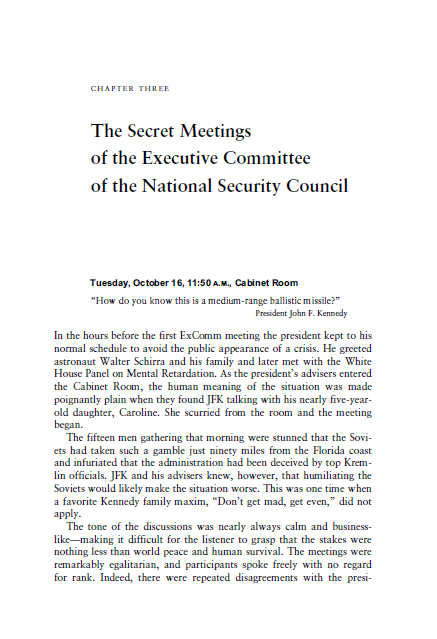
\includegraphics[width=0.48\textwidth]{./chapters/chapter51}\hfill
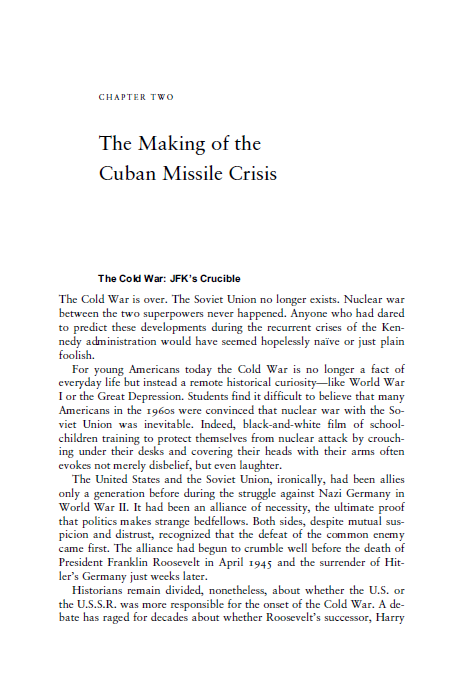
\includegraphics[width=0.48\textwidth]{./chapters/chapter51a}
\caption{Style 50 from the Oxford Handbook of Cuneiform Culture.}
\end{figure}

\section{Some notes}

If you observe this style carefully you will notice that the full title block, including the epigraph are set in from the left margin. This is achieved by setting appropriate \cs{hspace} lengths. The epigraph key width, needs to have the right distance and calculate the width. Example~ \ref{ch:style51} demonstrates the technique.

\begin{texexample}{Example setting-in the title block and epigraph}{ch:style51}
\cxset{style51,
   chapter opening=anywhere,
   epigraph align=right,
   epigraph width=\dimexpr(\textwidth-1.0cm)\relax,
  }
\chapter{Introduction to Chapter Style 51}
\epigraph{\textbf{\sffamily Tuesday, October 16, 11:50 \textsc{a.m}, Cabinet Room}\par
               ``How do you know this is a medium-range ballistic missile?''}{President John F. Kennedy}
\lorem
\end{texexample}

%% Style 52
% CHOMSKY

\cxset{
 name=CHAPTER,
 numbering=arabic,
 number font-size=\large,
 number before={},
 number position=rightname,
 chapter spaceout=soul,
 chapter color={black!80},
 chapter font-size=\large,
 chapter before=\rule[3pt]{\textwidth}{0.4pt}\par\hfill,
 number after=,
 chapter after=\hfill\hfill\par\vspace*{-3pt}\rule[3pt]{\textwidth}{0.4pt}\par,
 number color=\color{black!80},
 title font-family=\bfseries,
 title font-color=\color{black!80},
 title font-weight=,
 title font-size=\Huge,
 title before=\hfill,
 title after=\hfill\hfill,
 title beforeskip=\vspace*{1cm},
 title afterskip=\vspace*{1.5cm},
 epigraph width=0.85\textwidth,
 epigraph align=center,
 header style=empty}

\chapter{Introduction to Style Fifty Two}
\epigraph{In the late forties \ldots\ it seemed to many that the conquest of syntax finally lay open
before the profession.\par
\parindent1em
At the beginning of the fifties confidence was running high. \lorem
}{H. Allan Gleason}

\section{Looking for Mr. Goodstructure}
This is an unusual book with a rather unique style. The vertical rule is simple and breaks the monotony of a book that is heavy on text.
\begin{figure}[ht]
\centering
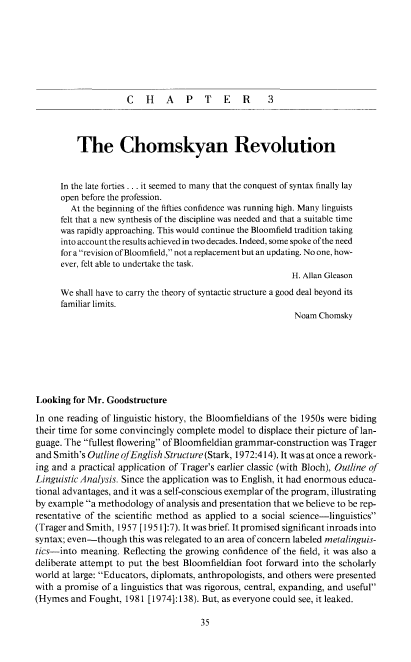
\includegraphics[width=0.35\textwidth]{./chapters/chapter52}
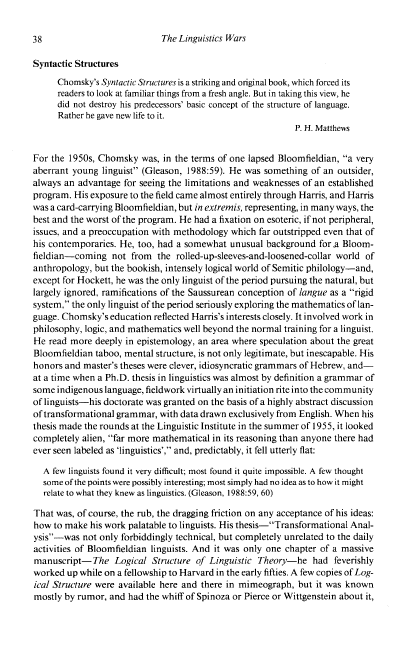
\includegraphics[width=0.35\textwidth]{./chapters/chapter52a}
\caption{Style 50 from the Oxford Handbook of Cuneiform Culture.}
\end{figure}

This style is very modern and typical of many computer books. The difficulty is in integrating all the page elements to make it work flawlessly.

THE
LINGUISTICS
WARS, RANDY ALLEN HARRIS

%% Style 53


\cxset{style53/.style={
 name=,
 numbering=arabic,
 number font-size=\Large,
 number before=\hfill,
 number after=\hfill\hfill\par\vspace*{1ex},
 number dot=,
 number position=rightname,
 number color=\color{blue},
 chapter color={blue},
 chapter font-size=\Large,
 chapter before=,
 chapter after=\par,
 title font-family=\rmfamily,
 title font-color=\color{blue},
 title font-weight=,
 title font-size=\LARGE,
 title before=\hfill,
 title after=\hfill\hfill,
 title beforeskip=,
 title afterskip=\leavevmode\center\rule{3cm}{0.4pt}\vskip-17pt\rule{3cm}{0.4pt}\endcenter\vskip10pt,
 header style=empty}}

\setstyle{53}
\pagestyle{fancy}
\chapter{{STYLE FIFTY THREE}}


This is an unusual book with a rather unique style. The vertical rule is simple and breaks the monotony of a book that is heavy on text. I also like the sky blue colour.
\begin{figure}[ht]
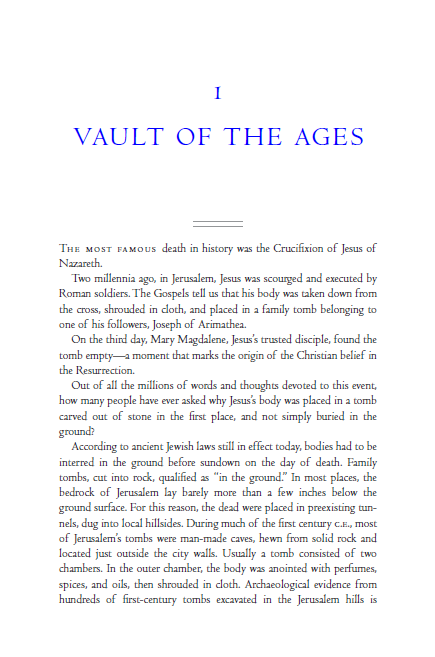
\includegraphics[width=0.48\textwidth]{./chapters/chapter53}\hfill
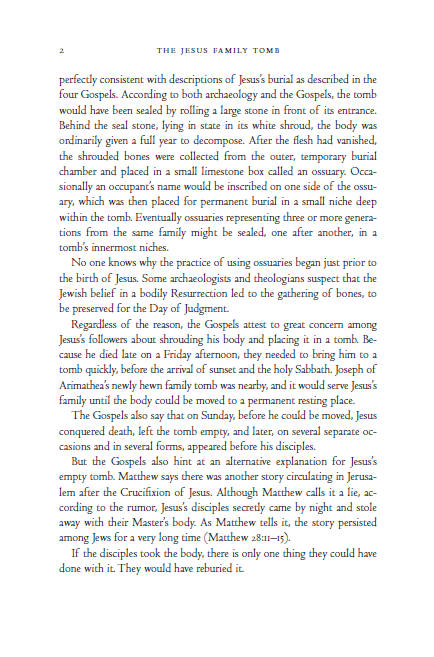
\includegraphics[width=0.48\textwidth]{./chapters/chapter53a}
\caption{Style 50 from the Oxford Handbook of Cuneiform Culture.}
\end{figure}

T h e
JESUS
FAMILY
TOMB
The Discovery, the Investigation,
and the Evidence
That Could Change History
SIMCHA JACOBOVICI and CHARLES PELLEGRINO

Harper Collins
\lipsum


%% Style 54

\cxset{appendix name/.store in=\appendix@cx}
\cxset{
 name=,
 numbering=arabic,
 number font-size=\Large,
 number before={},
 number after=,
 number dot=,
 number position=rightname,
 number color=\color{blue},
 chapter color={blue},
 chapter font-size=\Large,
 chapter before=\par\hfill\hfill,
 chapter after=\hfill,
 title font-family=\rmfamily,
 title font-color=\color{blue},
 title font-weight=,
 title font-size=\LARGE,
 title beforeskip=\hfill,
 title afterskip={\vspace*{20pt}},
 header style=empty}
\chapter{{STYLE FIFTY FOUR}}


This is an unusual book with a rather unique style. The vertical rule is simple and breaks the monotony of a book that is heavy on text.\index{rules!style 54}

\begin{figure}[ht]
\fbox{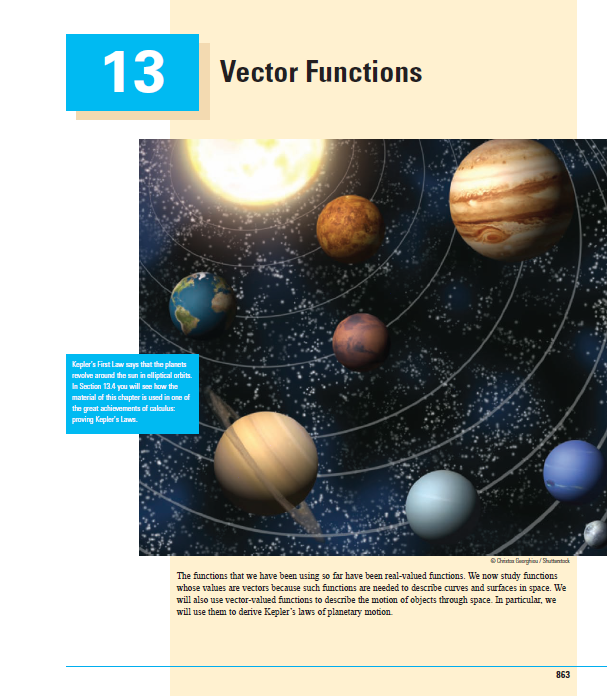
\includegraphics[width=0.48\textwidth]{./chapters/chapter54}}\hfill
\fbox{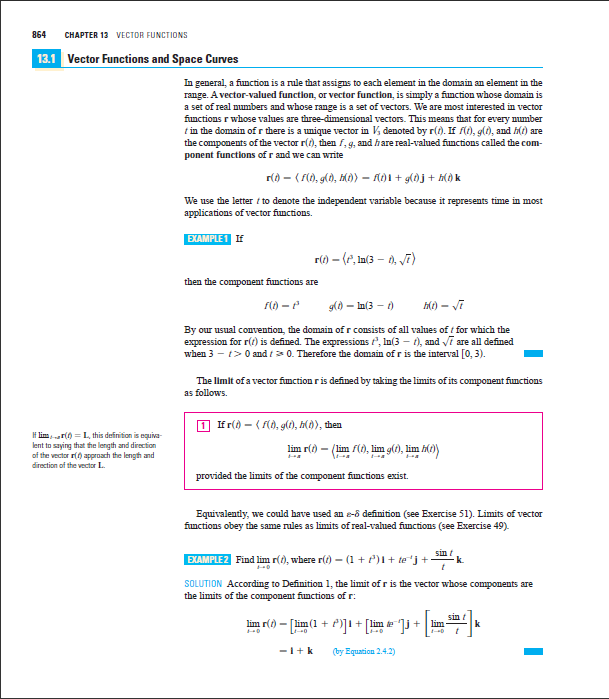
\includegraphics[width=0.48\textwidth]{./chapters/chapter54a}}
\caption{Style 50 from Steward's Calculus.}
\end{figure}

This style has already been discussed.

\@specialtrue
%\setstyle{53}
\cxset{appendix name/.code=\gdef\appendixname{#1}}

\cxset{steward,
  appendix name=Appendix,
  numbering=arabic,
  custom=tikzspecial,
  offsety=0cm,
  image=rainbow,
  texti={So far we have seen how to reset styles for the common sectioning commands, such as chapters and sections. Other common elements of a book such as an appendices are discussed here.},
  textii={We have already investigated some of the applications of derivatives, but now that we know the differentiation
rules we are in a better position to pursue the applications of differentiation in greater depth. Here
we learn how derivatives affect the shape of a graph of a function and, in particular, how they help us
locate maximum and minimum values of functions. Many practical problems require us to minimize a
cost or maximize an area or somehow find the best possible outcome of a situation. In particular, we will
be able to investigate the optimal shape of a can and to explain the location of rainbows in the skys.}
}

\appendix
\cxset{numbering=Alpha,
          section numbering=numeric}
\chapter{STYLING APPENDICES}

\section{Appendix section}

As far as LaTeX is concerned, there is nothing special in styling an appendix. It is either a chapter or a section with a different name. This name in order to allow internationalization is called \lstinline{appendixname}.
\bigskip

\begin{tcolorbox}[width=\linewidth]
\begin{lstlisting}
\newcommand\appendix{\par
  \setcounter{chapter}{0}%
  \setcounter{section}{0}%
  \gdef\@chapapp{\appendixname}(*@\footnote{The actual literal used for   \textbackslash{appendixname} is defined later on, so that you can customize the language}\label{appendixname}@*)
  \gdef\thechapter{\@Alph\c@chapter}
}
\end{lstlisting}
\end{tcolorbox}
\medskip

The code above is only a simplified version of the command. One might need to add more formatting information such as resetting equation numbers, tables and figures and any special floating environments that have their own numbering.

\begin{tcolorbox}[width=\linewidth]
\begin{lstlisting}
\renewcommand\appendix{\par
                \stepcounter{chapter}
                \setcounter{chapter}{0}
                \stepcounter{section}
                \setcounter{section}{0}
                \setcounter{equation}{0}
                \setcounter{figure}{0}
                \setcounter{table}{0}
                \setcounter{footnote}{0}
  \def\@chapapp{\appendixname}%
  \renewcommand\thechapter{\@Alph\c@chapter}}
\end{lstlisting}
\end{tcolorbox}


\section{Usage}

With the \lstinline{classx} package appendices are formatted as chapters.

\begin{tcolorbox}[width=\linewidth]
\begin{lstlisting}
\appendix
\cxset{numbering=Alpha}
\chapter{STYLING APPENDICES}
\end{lstlisting}
\end{tcolorbox}

\subsection{Enhancements}
More enhancements are possible. For one we can get rid of the chapter, which semantically is not very good, one should have followed a similar style to that of the sections and the \lstinline!\appendix{Title}!. I am not sure if this wouldn't be a bit confusing to people.

\subsubsection{Appendices at end of chapters}
Some styles require appendices to be set at the end of each chapter. These type of appendices can also be added. However an appendix counter might need to be defined.

\paragraph{test paragraph}

\subparagraph{test subparagraph}


%\setstyle{13}
\cxset{numbering=Alpha, name=Appendix}
\@specialfalse%required to negate effect of special tikz picture.

\chapter{Another Appendix}
\section{Calling appendix styles}
\lipsum[1-3]


\@specialtrue
\cxset{steward,
  appendix name=Appendix,
  numbering=Alpha,
  custom=tikzspecial,
  offsety=0cm,
  image=rainbow,
  texti={So far we have seen how to reset styles for the common sectioning commands, such as chapters and sections. Other common elements of a book such as an appendices are discussed here.},
  textii={We have already investigated some of the applications of derivatives, but now that we know the differentiation
rules we are in a better position to pursue the applications of differentiation in greater depth. Here
we learn how derivatives affect the shape of a graph of a function and, in particular, how they help us
locate maximum and minimum values of functions. Many practical problems require us to minimize a
cost or maximize an area or somehow find the best possible outcome of a situation. In particular, we will
be able to investigate the optimal shape of a can and to explain the location of rainbows in the sky.}
}

\chapter{The Special Environments\\Quotation and Quote}

\begin{quotation}
\lipsum[1-2]
\end{quotation}

\begin{figure}
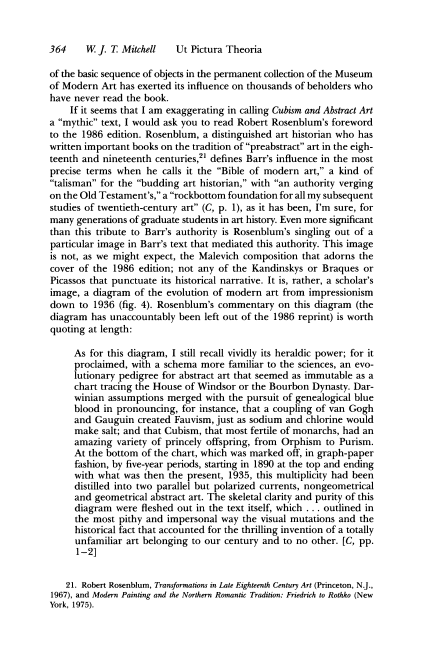
\includegraphics[width=0.9\linewidth]{quotations-01}
\caption{Most books have quotes flushed right.}
\end{figure}

%% Set the quotation environment
\cxset{
  quotation above/.store in=\quotationabove@cx,
  quotation left margin/.store in=\quotationleftmargin@cx,
  quotation right margin/.store in=\quotationrightmargin@cx,
  quotation parsep/.store in=\quotationparsep@cx,
  quotation font-size/.store in=\quotationfontsize@cx,
  quotation parindent/.store in=\quotationparindent@cx,
}

\def\setquotation#1{%
\cxset{#1}
\renewenvironment{quotation}
               {\par\addvspace{\quotationabove@cx}
                \list{}{\listparindent\quotationparindent@cx%
                        \leftmargin=\quotationleftmargin@cx%
                        \itemindent    \listparindent
                        \rightmargin   \leftmargin
                        \parsep=\quotationparsep@cx%
                        \quotationfontsize@cx}%
                \item\relax\hskip-\listparindent}
               {\endlist}
}

% Some default values
\setquotation{%
  quotation above=6pt,
  quotation left margin=20pt,
  quotation right margin=0pt,
  quotation parsep=0pt,
  quotation font-size=\small,
  quotation parindent=12pt,
}

%% Set the quote environment
\cxset{
  quote above/.store in=\quoteabove@cx,
  quote left margin/.store in=\quoteleftmargin@cx,
  quote right margin/.store in=\quoterightmargin@cx,
  quote parsep/.store in=\quoteparsep@cx,
  quote font-size/.store in=\quotefontsize@cx,
  quote parindent/.store in=\quoteparindent@cx,
}

\def\setquote#1{%
\cxset{#1}
\renewenvironment{quote}
               {\par\addvspace{\quoteabove@cx}
                \list{}{\listparindent\quoteparindent@cx%
                        \leftmargin=\quoteleftmargin@cx%
                        \itemindent    \listparindent
                        \rightmargin   \leftmargin
                        \parsep=\quoteparsep@cx%
                        \quotefontsize@cx}%
                \item\relax\hskip-\listparindent}
               {\endlist}
}

% Some default values
\setquotation{%
  quotation above=36pt,
  quotation left margin=50pt,
  quotation parsep=0pt,
  quotation font-size=\small,
  quotation parindent=12pt,
}
\setquote{%
  quote above=36pt,
  quote left margin=20pt,
  quote parsep=0pt,
  quote font-size=\small,
  quote parindent=12pt,
}

\section{Quotation}
In the standard \LaTeXe\ classes the quotation and quote environment are defined by making clever use of the list environment. The main difference between the quotation and the quote environment is that the first line of the former is indented. The key value interface for the quotation environment is shown below and a similar one exists for the quotation environment:

\section{Key-value interface}\index{quotation!keys}

\keyval{quote above}{\marg{dim}}{Skip dimension for above quotation skip.}
\keyval{quote below}{\marg{dim}}{Skip dimension for below quotation skip.}
\keyval{quote parindent}{\marg{dim}}{Paragraph indentation.}
\keyval{quote parsep}{\marg{dim}}{Paragraph below skip.}
\keyval{quote left margin}{\marg{dim}}{Paragraph below skip.}
\keyval{quote right margin}{\marg{dim}}{Paragraph below skip.}

\index{quotation!example}
\begin{tcblisting}{title=Quotation environment example,width=\textwidth}
\setquotation{%
  quotation above=36pt,
  quotation left margin=0pt,
  quotation right margin=0pt,
  quotation parsep=10pt,
  quotation font-size=\small,
  quotation parindent=1em,
}
\begin{quotation}
\lipsum[2-3]
\end{quotation}
\end{tcblisting}

\section{Quote}
This is the quote environment:
\begin{quote}
\lipsum[1-2]
\end{quote}


\@specialtrue
\cxset{steward,
  appendix name=Appendix,
  numbering=Alpha,
  custom=tikzspecial,
  offsety=0cm,
  image=sweepers,
  texti={Lists are essential elements of any document style and perhaps the most troublesome to get right.
         In this chapter we discuss the construction of lists and offer a key value interface.},
  textii={The Chapter discusses in detail the construction of lists. It reviews the mechanisms offered
          by LaTeX and outlines a key value approach to building lists. We define a standard interface that does not
          interfere with the original commands. The three standard list styles \textit{enumerate, itemize} and \textit{description} are redesigned to accept a key value interface. The photograph is Lewis Hine's which noted: ``Ivey Mill Company, Hickory, N.C. Some doffers and sweepers. Plenty of them.'' Location: Hickory, Catawba County Date: November 1908. Photographs like this were used by Hine to campaign against child labour.
         }
}

\chapter{Standard \LaTeX\ Lists}

%\tcbset{width=\linewidth,arc=1mm,before=\bigskip,after=\medskip,left=8mm}
The general parameters affecting a general list is shown in the  diagram  below\footnote{Produced using the \texttt{layouts} package.}. LaTeX offers three general list structures, enumerate, itemize and description.
\begin{figure}[hp]
\listdiagram
\caption{Layout of an \texttt{enumerate} list} \label{fig:lstenum}
\end{figure}

\section{Package usage}

List are set using setenumerate, setitemize, setdescription. It is also possible to create new list structures, which will be explained a bit later on.

\newpage
\section{The description list environment}
Unlike the enumerate and itemize environment, the description list environment is defined in the book class.
The environment is defined as:

\begin{tcolorbox}
\begin{lstlisting}
\newenvironment{description}
               {\list{}{\labelwidth\z@ \itemindent-\leftmargin
                        \let\makelabel\descriptionlabel}}
               {\endlist}
\newcommand*\descriptionlabel[1]{\hspace\labelsep\labelcolor@cx
                                \normalfont\bfseries #1}
\end{lstlisting}
\end{tcolorbox}

What is important to notice here is that all the standard list parameters are left essentially unchanged. The only item that is affected is \lstinline{\makelabel}, which is redefined in \lstinline{description} label.


We can define a number of keys for ease of formatting such descriptions lists rather than each time redefining them.


\begin{tcolorbox}[title=Basic description list keys]
\begin{lstlisting}
\cxset{
 description label font-size/.store in=\descriptionlabelfontsize@cx,
 description label font-weight/.store in=\descriptionlabelfontweight@cx,
 description label font-family/.store in=\descriptionlabelfontfamily@cx,
 description label font-shape/.store in=\descriptionfontshape@cx,
 description label color/.store in=\descriptionlabelcolor@cx,
 description label sep/.store in=\descriptionlabelsep@cx,
 description label width/.store in=\descriptionlabelwidth@cx,
 description margin left/.store in=\descriptionmarginleft@cx,
 description margin right/.store in=\descriptionmarginright@cx,
 description item indent/.store in=\descriptionitemindent@cx,
 list parindent/.store in=\descriptionlistparindent@cx,
}
\end{lstlisting}
\end{tcolorbox}

\cxset{
 description label font-size/.store in=\descriptionlabelfontsize@cx,
 description label font-weight/.store in=\descriptionlabelfontweight@cx,
 description label font-family/.store in=\descriptionlabelfontfamily@cx,
 description label font-shape/.store in=\descriptionlabelfontshape@cx,
 description label color/.store in=\descriptionlabelcolor@cx,
 description label sep/.store in=\descriptionlabelsep@cx,
 description label width/.store in=\descriptionlabelwidth@cx,
 description margin left/.store in=\descriptionmarginleft@cx,
 description margin right/.store in=\descriptionmarginright@cx,
 description item indent/.store in=\descriptionitemindent@cx,
 list parindent/.store in=\descriptionlistparindent@cx,
}

We also define a macro \lstinline{\setdescription} as a helper macro to assist in changing settings at any point in a document.

\begin{tcolorbox}[title=Basic description list keys]
\begin{lstlisting}
\def\setdescription#1{%
\cxset{#1}%
\renewenvironment{description}%
{\list{}{\listparindent\descriptionlistparindent@cx%
                       \leftmargin=\descriptionmarginleft@cx%
                       \rightmargin=\descriptionmarginright@cx%
                       \itemindent\descriptionitemindent@cx%
                       \labelwidth\descriptionlabelwidth@cx%
                       \labelsep=\descriptionlabelsep@cx%
                       \let\makelabel\descriptionlabel}}%
               {\endlist}%
%
\renewcommand\descriptionlabel[1]{%
  \fboxrule0pt\fboxsep0pt%
  \hspace\descriptionlabelsep@cx%\labelsep%
  \fbox{\color{\descriptionlabelcolor@cx}%
  \normalfont\bfseries\raggedleft##1\thickspace%
}}%
}
\end{lstlisting}
\end{tcolorbox}


\def\setdescription#1{%
\cxset{#1}%
\renewenvironment{description}%
{\list{}{\listparindent\descriptionlistparindent@cx%
                       \leftmargin=\descriptionmarginleft@cx%
                       \rightmargin=\descriptionmarginright@cx%
                       \itemindent\descriptionitemindent@cx%
                       \labelwidth\descriptionlabelwidth@cx%
                       \labelsep=\descriptionlabelsep@cx%
                       \let\makelabel\descriptionlabel}}%
               {\endlist}%
%
\renewcommand\descriptionlabel[1]{%
  \fboxrule0pt\fboxsep0pt%
  \hspace\descriptionlabelsep@cx%\labelsep%
  \fbox{\color{\descriptionlabelcolor@cx}%
  \normalfont\bfseries\raggedleft##1\thickspace%
}}%
}
\setdescription{%
 description label font-size=\normalfont,
 description label font-weight=\bfseries,
 description label font-family=\sffamily,
 description label font-shape=\itshape,
 description label color=purple,
 description label sep=0sp\relax,
 description label width=100pt,
 description margin left=20pt,
 description margin right=20pt,
 description item indent=90pt,
 list parindent=1em,
}

\section{Creating new description like environments}

The macro \lstinline{\newdescriptionenvironment} can be used to redefine new description like environments.

\begin{tcblisting}{title=Example: define new description list environment}
\def\newdescriptionenvironment#1#2{%
\cxset{#2}%
\newenvironment{#1}%
{\list{}{\listparindent\descriptionlistparindent@cx%
                       \leftmargin=\descriptionmarginleft@cx%
                       \rightmargin=\descriptionmarginright@cx%
                       \itemindent\descriptionitemindent@cx%
                       \labelwidth\descriptionlabelwidth@cx%
                       \labelsep=\descriptionlabelsep@cx%
                       \let\makelabel\descriptionlabel}}%
               {\endlist}%
%
\renewcommand\descriptionlabel[1]{%
  \fboxrule0pt\fboxsep0pt%
  \hspace\descriptionlabelsep@cx%\labelsep%
  \fbox{\color{\descriptionlabelcolor@cx}%
  \descriptionlabelfontsize@cx%
  \descriptionlabelfontweight@cx%
  \descriptionlabelfontfamily@cx%
  \descriptionlabelfontshape@cx%
  \hbox to \labelwidth{\hfill##1}%
}}%
}
\newdescriptionenvironment{orangedescription}{
 description label font-size=\normalfont,
 description label font-weight=\bfseries,
 description label font-family=\sffamily,
 description label font-shape=\itshape,
 description label color=orange,
 description label sep=3.5pt\relax,
 description label width=40pt,
 description margin left=50pt,
 description margin right=20pt,
 description item indent=-2.5pt,
 list parindent=1em,
}
The \texttt{orangedescription} environment in action.
\begin{orangedescription}
 \item[One] \lorem
 \item[Two] \lorem
 \item[Three] \lorem
\end{orangedescription}
\end{tcblisting}

\newpage

\section{Example: redefining a description list}
We will now develop a description environment, that can be useful for the documentation of packages to describe options. We will use a description list as the basis of the environment. We define the following key values.

\begin{description}
\item[description label font-size]This is the first item.
\item[description label font-weight]This is the second item. \lipsum*[1]
\item[description label font-family] This is the font family.
\item[description label font-shape] This is the font family.
\item[description label color] This is the font family.
\item[description label sep] The space between the description label and the description text.
\item [description label width] The space between the description label and the description text.
[description margin left] The space between the list indentation and the left margin.
\lipsum*[3]
\end{description}



\savegeometry{default}

\section{Enumerated lists}


\begin{enumerate}
\item one
\item two
\item three
\end{enumerate}

Enumerated (numbered) list environments are characterized by numbering. They use a variety of fields and counters as shown in table.

\subsection{Vertical skips}

By default LaTeX adds vertical skips, as shown in figure 1. The definition of these skips is influenced by the font size and are defined in the \texttt{bk10.clo} files, hence hard to find and change. Each level of the list has its own definition as \lstinline{\@listi}.

\bigskip
\tcbset{width=\linewidth,arc=1mm,before=\bigskip,left=8mm}

\begin{tcolorbox}[title=Extract from bk10.clo]
\begin{lstlisting}
\def\@listi{\leftmargin\leftmargini
            \parsep 4\p@ \@plus2\p@ \@minus\p@
            \topsep 8\p@ \@plus2\p@ \@minus4\p@
            \itemsep4\p@ \@plus2\p@ \@minus\p@}
\let\@listI\@listi
\@listi
\def\@listii {\leftmargin\leftmarginii
              \labelwidth\leftmarginii
              \advance\labelwidth-\labelsep
              \topsep    4\p@ \@plus2\p@ \@minus\p@
              \parsep    2\p@ \@plus\p@  \@minus\p@
              \itemsep   \parsep}
\def\@listiii{\leftmargin\leftmarginiii
              \labelwidth\leftmarginiii
              \advance\labelwidth-\labelsep
              \topsep    2\p@ \@plus\p@\@minus\p@
              \parsep    \z@
              \partopsep \p@ \@plus\z@ \@minus\p@
              \itemsep   \topsep}
\def\@listiv {\leftmargin\leftmarginiv
              \labelwidth\leftmarginiv
              \advance\labelwidth-\labelsep}
\def\@listv  {\leftmargin\leftmarginv
              \labelwidth\leftmarginv
              \advance\labelwidth-\labelsep}
\def\@listvi {\leftmargin\leftmarginvi
              \labelwidth\leftmarginvi
              \advance\labelwidth-\labelsep}
\end{lstlisting}
\end{tcolorbox}


\cxset{enumerate numberingi/.is choice,
  enumerate numberingi/.code={\renewcommand\theenumi {\csname#1\endcsname{enumi}}},
  enumerate numberingii/.code={\renewcommand\theenumii {\csname#1\endcsname{enumii}}},
  enumerate numberingiii/.code={\renewcommand\theenumiii {\csname#1\endcsname{enumiii}}},
  enumerate numberingiv/.code={\renewcommand\theenumiv {\csname#1\endcsname{enumiv}}},
 % labels
  enumerate labeli punctuation/.store in=\enumeratepunctuationi@cx,
  enumerate labeli/.is choice,
  enumerate labeli/brackets/.code={\renewcommand\labelenumi{(\theenumi\enumeratepunctuationi@cx)}},
  enumerate labeli/square brackets/.code={\renewcommand\labelenumi{[\theenumi\enumeratepunctuationi@cx]}},
  enumerate labeli/right bracket/.code={\renewcommand\labelenumi{\theenumi\enumeratepunctuationi@cx)}},
  enumerate label left/.store in=\enumeratelabelleft@cx,
  enumerate label right/.code=\renewcommand\labelenumi{\enumeratelabelleft@cx\theenumi\enumeratepunctuationi@cx#1},
  enumerate leftmargini/.code={\setlength\leftmargini{#1}},
  enumerate leftmarginii/.code={\setlength\leftmarginii{#1}},
  enumerate leftmarginiii/.code={\setlength\leftmarginiii{#1}},
  enumerate leftmarginiv/.code={\setlength\leftmarginiv{#1}},
  listi topsep/.store in=\listitopsep@cx,
  listi partopsep/.store in=\listipartopsep@cx,
  listi itemsep/.store in=\listiitemsep@cx,
  listi parsep/.store in=\listiparsep@cx,
% second level
  listii topsep/.store in=\listiitopsep@cx,
  listii partopsep/.store in=\listiipartopsep@cx,
  listii itemsep/.store in=\listiiitemsep@cx,
  listii parsep/.store in=\listiiparsep@cx,
% third level
  listiii topsep/.store in=\listiiitopsep@cx,
  listiii partopsep/.store in=\listiiipartopsep@cx,
  listiii itemsep/.store in=\listiiiitemsep@cx,
  listiii parsep/.store in=\listiiiparsep@cx,
}

\cxset{compact1/.style={%
  enumerate numberingi=arabic,
  enumerate numberingii=alph,
  enumerate numberingiii=alph,
  enumerate numberingiv=roman,
  enumerate labeli punctuation=.,
  enumerate label left=,
  enumerate label right=,
  enumerate leftmargini=2.2em,
  enumerate leftmarginii=2.1em,
  enumerate leftmarginiii=1.5em,
  enumerate leftmarginiv=2em,
% override some of the .clo defaults
  listi topsep=8\p@ \@plus2\p@ \@minus\p@,
  listi itemsep=0\p@ \@plus2\p@ \@minus\p@,
  listi parsep=0\p@ \@plus2\p@ \@minus\p@,
% second level
  listii topsep=0\p@ \@plus2\p@ \@minus\p@,
  listii itemsep=0\p@ \@plus2\p@ \@minus\p@,
  listii parsep=0\p@ \@plus2\p@ \@minus\p@,
% third level
  listiii topsep=0\p@ \@plus2\p@ \@minus\p@,
  listiii itemsep=0\p@ \@plus2\p@ \@minus\p@,
  listiii parsep=0\p@ \@plus2\p@ \@minus\p@,
}}

\cxset{compact2/.style={%
  enumerate numberingi=alph,
  enumerate numberingii=roman,
  enumerate numberingiii=alph,
  enumerate numberingiv=roman,
  enumerate labeli punctuation=,
  enumerate label left=(,
  enumerate label right=),
  enumerate leftmargini=2.2em,
  enumerate leftmarginii=2.1em,
  enumerate leftmarginiii=1.5em,
  enumerate leftmarginiv=2em,
% override some of the .clo defaults
  listi topsep=8\p@ \@plus2\p@ \@minus\p@,
  listi itemsep=0\p@ \@plus2\p@ \@minus\p@,
  listi parsep=0\p@ \@plus2\p@ \@minus\p@,
% second level
  listii topsep=0\p@ \@plus2\p@ \@minus\p@,
  listii itemsep=0\p@ \@plus2\p@ \@minus\p@,
  listii parsep=0\p@ \@plus2\p@ \@minus\p@,
% third level
  listiii topsep=0\p@ \@plus2\p@ \@minus\p@,
  listiii itemsep=0\p@ \@plus2\p@ \@minus\p@,
  listiii parsep=0\p@ \@plus2\p@ \@minus\p@,
}}


\def\setenumerate#1{
\cxset{#1}
\def\@listi{\leftmargin\leftmargini
            \parsep\listiparsep@cx
            \topsep\listitopsep@cx\relax
            \itemsep\listiitemsep@cx}
\def\@listii{\leftmargin\leftmarginii
            \parsep\listiiparsep@cx
            \topsep\listiitopsep@cx\relax
            \itemsep\listiiitemsep@cx}
\def\@listiii{\leftmargin\leftmarginiii
            \parsep\listiiiparsep@cx
            \topsep\listiiitopsep@cx\relax
            \itemsep\listiiiitemsep@cx}
}

\setenumerate{compact1}


The list can be viewed here:

\begin{enumerate}
\item Level i
      \begin{enumerate}
       \item Level ii
          \begin{enumerate}
            \item Level iii
              \begin{enumerate}
                \item Level iv. \lipsum*[1]
              \end{enumerate}
          \end{enumerate}
      \end{enumerate}
\end{enumerate}


\begin{tcblisting}{title=Example with style \textit{compact2}}
% Define the style
\cxset{compact2/.style={%
  enumerate numberingi=alph,
  enumerate numberingii=roman,
  enumerate numberingiii=alph,
  enumerate numberingiv=roman,
  enumerate labeli punctuation=,
  enumerate label left=(,
  enumerate label right=),
  enumerate leftmargini=2.2em,
  enumerate leftmarginii=2.1em,
  enumerate leftmarginiii=1.5em,
  enumerate leftmarginiv=2em,
% override some of the .clo defaults
  listi topsep=8\p@ \@plus2\p@ \@minus\p@,
  listi itemsep=0\p@ \@plus2\p@ \@minus\p@,
  listi parsep=0\p@ \@plus2\p@ \@minus\p@,
% second level
  listii topsep=0\p@ \@plus2\p@ \@minus\p@,
  listii itemsep=0\p@ \@plus2\p@ \@minus\p@,
  listii parsep=0\p@ \@plus2\p@ \@minus\p@,
% third level
  listiii topsep=0\p@ \@plus2\p@ \@minus\p@,
  listiii itemsep=0\p@ \@plus2\p@ \@minus\p@,
  listiii parsep=0\p@ \@plus2\p@ \@minus\p@,
}}
\setenumerate{compact2}
\begin{enumerate}
\item Does this project actually merit the use of the Minor Works Form or Intermediate Form instead of their `grown up' relatives?
\item Do the number of PC or prime cost items mean that it would be more desirable to use a re-measurable form?
\item Is this a contract which merits the production of full scale bills
of quantities or is something more standardised going to suffice?
\end{enumerate}
\end{tcblisting}

As you will observe the numbering in the above example has been enclosed in round brackets, using:

\begin{tcolorbox}
\begin{lstlisting}
  enumerate label left=(,
  enumerate label right=),
\end{lstlisting}
\end{tcolorbox}

The next example is from the \textit{LaTeX Companion}. In example~\ref{ex:companion}, the first-level list elements are decorated with the section sign (\S) as a prefix and a period as a suffix (omitted in references). We will
define this as a style named \textit{paragraphsymbol} for the lack of any better name. This style can sometimes be found in legal texts.

\begin{texexample}{Paragraph symbols in enumerate}{ex:companion}
\cxset{paragraphsymbol/.style={%
  enumerate numberingi=arabic,
  enumerate labeli punctuation=.,
  enumerate label left=\S,
  enumerate label right=,
}}
\setenumerate{paragraphsymbol}
\begin{enumerate}
\item \lorem
\item \lorem
\item \lorem
\end{enumerate}
\end{texexample}

\section{Creating enumerated environments}

New enumerated environments cab be created by using the macro \lstinline{\newenumeratedenvironment}. Keys are set as either styles or individually.

\def\newenumeratedenvironment#1#2{%
 \expandafter\def\csname#1\endcsname{%
 \cxset{#2}
 \ifnum \@enumdepth >\thr@@\@toodeep\else
 \advance\@enumdepth\@ne
 \edef\@enumctr{enum\romannumeral\the\@enumdepth}%
 \expandafter
 \list
 \csname label\@enumctr\endcsname
 {\usecounter\@enumctr\def\makelabel####1{\hss\llap{####1}}}%
 \fi}
 \expandafter\let\csname end#1\endcsname=\endlist
}


\begin{texexample}{An enumerated list factory}{}
\newenumeratedenvironment{paragraphsymbol}{
  enumerate numberingi=arabic,
  enumerate labeli punctuation=.,
  enumerate label left={\textcolor{purple}{\P}},
  enumerate label right=,
}
\begin{paragraphsymbol}
\item \lorem
\item \lorem
\item \lorem
      \begin{itemize}
        \item This is bullets
      \end{itemize}
\end{paragraphsymbol}
\end{texexample}


\newpage
\section{Setup keys for enumerate lists}
\begin{description}
\item [enumerate numberingi] Sets the numbering style of the list at level $n$. Valid values are \textit{Alph, alph, arabic, Roman, roman, WORDS, words}.
\end{description}

\clearpage

\section{Itemized lists}

The itemized \LaTeX\ lists are similar to those for the enumerated lists. However they are somehow simpler as there is no need for counters.

\bigskip
\begin{tcolorbox}[width=\linewidth,arc=2mm,title=Default \LaTeX\ parameters for itemized lists]
\begin{lstlisting}
\newcommand\labelitemi{\textbullet}
\newcommand\labelitemii{\normalfont\bfseries \textendash}
\newcommand\labelitemiii{\textasteriskcentered}
\newcommand\labelitemiv{\textperiodcentered}
\end{lstlisting}
\end{tcolorbox}

\cxset{
 labelitemi/.code=\def\labelitemi{#1},
 labelitemii/.code=\def\labelitemii{#1},
 labelitemiii/.code=\def\labelitemiii{#1},
 labelitemiv/.code=\def\labelitemiv{#1},
}

\cxset{
 labelitemi={{\color{red}\ding{"E4}}},
 labelitemii=\textendash,
 labelitemiii=\textasteriskcentered,
 labelitemiv=\textperiodcentered,
}



\begin{itemize}
\item Level i
      \begin{itemize}
       \item Level ii
          \begin{itemize}
            \item Level iii
              \begin{itemize}
                \item Level iv. \lipsum*[1]
              \end{itemize}
          \end{itemize}
      \end{itemize}
\end{itemize}

\cxset{red/.style={
 labelitemi={{\color{green}\ding{'64}}},
 labelitemii=\color{red}\textendash,
 labelitemiii=\textasteriskcentered,
 labelitemiv=\textperiodcentered,
}}

Now that we have managed to abstract the itemized environment we can generate a new environment factory.

\def\newitemizedenvironment#1#2{
\expandafter\def\csname#1\endcsname{%
 \cxset{#2}%
 \ifnum \@itemdepth >\thr@@\@toodeep\else
 \advance\@itemdepth\@ne
 \edef\@itemitem{labelitem\romannumeral\the\@itemdepth}%
 \expandafter
 \list
 \csname\@itemitem\endcsname
 {\def\makelabel####1{\hss\llap{####1}}}%
 \fi}
 \expandafter\let\csname end#1\endcsname=\endlist
}

\newitemizedenvironment{reditemize}{red}


\begin{reditemize}
\item Test.
   \begin{reditemize}
    \item test.
   \end{reditemize}
\end{reditemize}

\begin{itemize}
\item Level i
      \begin{itemize}
       \item Level ii
          \begin{itemize}
            \item Level iii
              \begin{itemize}
                \item Level iv. \lipsum*[1]
              \end{itemize}
          \end{itemize}
      \end{itemize}
\end{itemize}


\section{Itemized lists with ding symbols}

So far we have used both standard symbols as well as those provided by the pifont that offers numerous,
dingbang symbols. The pifont package also offers environments to do that more easily.


\begin{texexample}{dinglist}{}
\begin{dinglist}{"E4}
\item The first item. \item The second
item in the list.
\end{dinglist}
\end{texexample}

\begin{dingautolist}{'300}
\item The first item in the list.\label{lst:a}
\item The second item in the list.\label{lst:b}
\item The third item in the list.\label{lst:c}
\end{dingautolist}

%%% DOCUMENATION MACROS


%% note becareful with styles here

\thispagestyle{plain}
\cxset{image=breakerboys}
\chapter{Documentation}


\section{Documentation macros}

When developing this package the need arose to define a number of documentation macros. I have used heavily macros and ideas present in the doc package, pgf documentation, biblatex documentation  and tcolorbox and for which I am grateful to their respective authors. The major change was to adopt the macros to use different fonts and colors and to use these from a list of key values defined at document level. More about this later. General package user documentation as opposed to package documentation that can be achieved using the doc/docstrip system requires that macros and environments be developed for the following:

\begin{enumerate}
\item Macros for command documentation.
\item Environments for commands and options.
\item Latex examples that need to be executed within the document as well as described.
\end{enumerate}

\subsection{Color management}
One of the first requirements for redefining some of the standard doc commands is the need to use color easily, hence we will try and define a certain amount of keys for colors.

Just a bit of a refresher, to define colors we use, either the \cs{definecolor} or the \cs{colorlet} commands.

\emphasis{definecolor,colorlet}
\begin{tcolorbox}
\begin{lstlisting}
% used for hyperlinks
\definecolor{Hyperlink}{rgb}{0.281,0.275,0.485}
\colorlet{thehyperlink}{theblue}
\end{lstlisting}
\end{tcolorbox}

We use a semantic approach, where the colors are first defined with a mnemonic command such as {\bfseries\textcolor{theblue}{theblue}} and then we define a semantic command such as the\cs{option} that lets the color to the option command. This sort of double entry has proved useful in navigating through the dozen of the commands that I needed for this documentation.

%\definecolor{theblue} {rgb}{0.02,0.04,0.48}
%\definecolor{thered}  {rgb}{0.65,0.04,0.07}
%\definecolor{thegreen}{rgb}{0.06,0.44,0.08}
%\definecolor{thelightgreen}{rgb}{0.06,0.44,0.06}
%\definecolor{thegrey} {gray}{0.5}
%\definecolor{thegrey} {gray}{0.5}
%\definecolor{theshade}{gray}{0.94}
%\definecolor{theframe}{gray}{0.75}
%\definecolor{thecream}{rgb}{1,0.95,0.4}
%\definecolor{spot}{rgb}{0,0.2,0.6}
%\definecolor{boxframe}{gray}{0.8}
%\definecolor{boxfill}{rgb}{0.95,0.95,0.99}
%\definecolor{theoption}{rgb}{0.118,0.546,0.222}
%\definecolor{themacro}{rgb}{0.784,0.06,0.176}
%\definecolor{ExampleFrame}{rgb}{0.628,0.705,0.942}
%\definecolor{ExampleBack}{rgb}{0.963,0.971,0.994}
%\definecolor{Hyperlink}{rgb}{0.281,0.275,0.485}
%\colorlet{thehyperlink}{theblue}
%\newcommand*{\defaultcolor}{\color{black}}
%\newcommand*{\spotcolor}{\color{spot}}

\subsection{Semantic color names}
\begin{marglist}
\item [\option{theoption}] Coloring of options in margin lists.
\item [\option{themacro}] Coloring of command macros \cs{foo}.
\item [\option{hyperlink}] If we use the \texttt{hyperref} package a number of colors need to be defined for links.
\end{marglist}

\subsection{Named colors}
Standard colors that we provide are:
\begin{marglist}
\item [\textcolor{theblue}{theblue}] This color is used mainly for options.
\item [\textcolor{thered}{thered}] The color mostly used for macro commands and keys.
\item [\textcolor{thegreen}{thegreen}] used for environments.
\item [\textcolor{thelightgreen}{thelightgreen}] Used for margin lists.
\item [\textcolor{thegray}{thegray}] Used as a background to the listings.
\item [\colorbox{thegrey}{\color{white}thegrey}] Alias for the gray to satisfy both sides of the Atlantic and as I sometimes don't remeber which is which.
\item [\colorbox{theshade}{theshade}] Another slightly lighter shade.
\end{marglist}



\begin{marglist}
\item [\cs{cs}] \cs{cs}\marg{text} Prints a command.
\item [\cs{cmd}] \cmd{\cmd}\marg{\cmd{\foo}} Prints a command.
\end{marglist}




\section{Lists for documentation}



The environment \env{marglist}
\begin{marglist}
\item[testing]\lorem
\item [test]\lorem
\end{marglist}

\env{keymarginlist}This environment is suitable for listing keys, set-in the margin.

\begin{keymarglist}
\item[bibliography] The term <bibliography>, also available as \cmd{bibname}.
\item[references] The term <references>, also available as \cmd{refname}.
\item[shorthands] The term <list of shorthands> or <list of abbreviations>, also available as \cmd{losname}.
\end{keymarglist}


\env{argumentlist} This environment is suitable for listing macro arguments and their explanations.

\newenvironment*{argumentlist}[1]
  {\list{}{%
     \settowidth{\labelwidth}{\displayverbfont#1}%
     \setlength{\labelsep}{1em}%
     \setlength{\leftmargin}{\labelwidth}%
     \addtolength{\leftmargin}{\labelsep}%
     \setlength{\itemsep}{0pt}%
     \renewcommand*{\makelabel}[1]{\displayverbfont##1\hss}}}
  {\endlist}

\begin{argumentlist}{00}
\item[\#1] The last names. If a name consists of a single part only (for example, <Aristotle>), this part will be treated as the last name.
\item[\#2] The last names, given as initials.
\item[\#3] The first names. This argument also includes all middle names.
\end{argumentlist}

\begin{tabular}{ll}
\env{marglist} & description list\\
\end{tabular}


\section{Future improvements}

Future improvements will involve defining additional environments and styles to integrate styles to those provided for chapters. Treat the code so far as a proof of concept experiment. It is also possible to improve on the code by utilizing some of the common packages.




\newpage






\@specialtrue
\cxset{steward,
  appendix name=Appendix,
  numbering=Alpha,
  custom=tikzspecial,
  offsety=0cm,
  image=doffer,
  texti={Backmatter material should follow the style set by the book chapters. Escaping from standard LaTeX formatting is as easy as making some simple changes to thebibliography environment.},
  textii={We have already investigated some of the applications of derivatives, but now that we know the differentiation
rules we are in a better position to pursue the applications of differentiation in greater depth. Here
we learn how derivatives affect the shape of a graph of a function and, in particular, how they help us
locate maximum and minimum values of functions. Many practical problems require us to minimize a
cost or maximize an area or somehow find the best possible outcome of a situation. In particular, we will
be able to investigate the optimal shape of a can and to explain the location of rainbows in the sky.}
}

\chapter{\bibname}
This can only be a small introduction to LaTeX's bibliography style modifications and we will only focus on the opening style.

\parindent1em

The standard \LaTeX\ environment for generating a list of references is called the \verb+thebibliography+ \cite{GOOSSENS94}. In its default implementation it automatically
generates an appropriate heading and implements a vertical list structure in which every publication is represented as a separate item.

\begin{tcolorbox}[title=LaTeX default thebibliography environment.]
\begin{lstlisting}
\newdimen\bibindent
\setlength\bibindent{1.5em}
\renewenvironment{thebibliography}[1]
     {%\chapter{\bibname}%
      \@mkboth{\MakeUppercase\bibname}{\MakeUppercase\bibname}%
      \list{\@biblabel{\@arabic\c@enumiv}}%
           {\settowidth\labelwidth{\@biblabel{#1}}%
            \leftmargin\labelwidth
            \advance\leftmargin\labelsep
            \@openbib@code
            \usecounter{enumiv}%
            \let\p@enumiv\@empty
            \renewcommand\theenumiv{\@arabic\c@enumiv}}%
      \sloppy
      \clubpenalty4000
      \@clubpenalty \clubpenalty
      \widowpenalty4000%
      \sfcode`\.\@m}
     {\def\@noitemerr
       {\@latex@warning{Empty `thebibliography' environment}}%
      \endlist}
\renewcommand\newblock{\hskip .11em\@plus.33em\@minus.07em}
\let\@openbib@code\@empty
\end{lstlisting}
\end{tcolorbox}

As you can observe the environment uses a list structure to produce the bibliography entries. As a matter of interest the environment uses a counter from the enumerate environment to save the use of an extra counter (\texttt{enumiv})\cite{source2e}.

Our only contribution here is to redefine the command slightly so that we can call a numbered or unnumbered chapter heading. Since we did all the appendices in a special chapter format, we kept the same style for all.\cite{companion}



%\newdimen\bibindent
%\setlength\bibindent{1.5em}
%\renewenvironment{thebibliography}[1]
%     {%\chapter{\bibname}%
%      \@mkboth{\MakeUppercase\bibname}{\MakeUppercase\bibname}%
%      \list{\@biblabel{\@arabic\c@enumiv}}%
%           {\settowidth\labelwidth{\@biblabel{#1}}%
%            \leftmargin\labelwidth
%            \advance\leftmargin\labelsep
%            \@openbib@code
%            \usecounter{enumiv}%
%            \let\p@enumiv\@empty
%            \renewcommand\theenumiv{\@arabic\c@enumiv}}%
%      \sloppy
%      \clubpenalty4000
%      \@clubpenalty \clubpenalty
%      \widowpenalty4000%
%      \sfcode`\.\@m}
%     {\def\@noitemerr
%       {\@latex@warning{Empty `thebibliography' environment}}%
%      \endlist}
%\renewcommand\newblock{\hskip .11em\@plus.33em\@minus.07em}
%\let\@openbib@code\@empty

%% some references used
%\begin{thebibliography}{GMS94}
%
%\bibitem[GMS94]{GOOSSENS94}
%Michel Goossens, Frank Mittelbach, and Alexander Samarin.
%\newblock \emph{The LaTeX Companion}.
%\newblock Addison-Wesley Publishing Company, 1994.
%
%\bibitem[Lam94]{LAMPORT94}
%Leslie Lamport.
%\newblock \emph{LaTeX: A Document Preparation System}.
%\newblock Addison-Wesley Publishing Company, second edition, 1994.
%
%\bibitem[McP88]{MCPHERSON88}
%Kent McPherson.
%\newblock `{Page Layout in LaTeX}'.
%\newblock \emph{TUGboat}, 9(1):78--82, April 1988.
%
%\bibitem[Wil02]{MEMOIR}
%Peter Wilson.
%\newblock \emph{The memoir class for configurable book typesetting}.
%\newblock November, 2002.
%\newblock (Available from CTAN in
%           \texttt{macros/latex/contrib/memoir})
%
%\bibitem[FM04]{source2e}
%Michel Goossens, Frank Mittelbach, and Alexander Samarin.
%\newblock \emph{The LaTeX source2e}.
%\newblock (Available from CTAN in
%            \texttt{macros/core/latex}.
%\end{thebibliography}

\cite[59]{companion}
\cite[see][]{companion}
\cite[see][59--63]{companion}

\section{Using Biblatex}

When you use biblatex rather than the default LaTeX styles--and you should--it is easier to get the formatting you want as the \cs{printbibliography} comes with its own set of keys.


\nocite{*}
\printbibliography[title=REFERENCES]

\printindex
\end{document}
https://docs.google.com/open?id=0B75n0wtctw00RDhYSkIwOTBRRHU5Rl93Q19lalRlQQ

%% Note with new geometry paper has to be defined in preamble
% I do not feel very confident of this
% Don't understand it fully how is working
 %\@twosidefalse \@mparswitchfalse % one side option
\cxset{geometry oxford/.code={
\newgeometry{left=74.8mm,top=27.4mm,headsep=2\baselineskip,%
marginparsep=8.2mm,marginparwidth=49.4mm,textheight=49\baselineskip,headheight=\baselineskip}
\@twosidefalse \@mparswitchfalse % one side option
\reversemarginpar
}}

\cxset{geometry textwidth/.store in=\textwidth@cx,
          geometry textheight/.store in=\textheight@cx,
          geometry tufte/.code={
             \newgeometry{a4paper,left=24.8mm,top=27.4mm,headsep=2\baselineskip,%
             textwidth=107mm,marginparsep=8.2mm,marginparwidth=49.4mm,%
             textheight=\textheight@cx\baselineskip,headheight=\baselineskip}
            \@twosidefalse \@mparswitchfalse % one side option
           %\reversemarginpar
    }
}


\cxset{marginpar push/.store in=\marginparpush@cx,
          marginpar font/.store in=\marginparfont@cx,
          marginpar justification/.is choice,
          marginpar justification/justifying/.code=\gdef\marginparjustification@cx{\justifying},
          marginpar justification/raggedright/.code=\gdef\marginparjustification@cx{\raggedright},
          marginpar justification/RaggedRight/.code=\gdef\marginparjustification@cx{\RaggedRight},
          marginpar justification/RaggedLeft/.code=\gdef\marginparjustification@cx{\RaggedLeft},
 }
\cxset{marginpar push=10pt,
          marginpar font=\normalfont\footnotesize\sffamily,
          marginpar justification=RaggedLeft}

\cxset{style13, geometry textheight=47,
          geometry tufte,
          watermark text=SAMPLE TUFTE VARIANT,
          watermark text color=thered,
          header style=samplepage}

\@ifundefined{stockheight}{\newlength\stockheight}{}
\@ifundefined{stockwidth}{\newlength\stockwidth}{}

% This is a sidenote without the footnote mark
\newcommand\marginnote[2][0pt]{%
 % \let\cite\@tufte@infootnote@cite%   use the in-sidenote \cite command
  %\gdef\@tufte@citations{}%           clear out any old citations
  \@tufte@margin@par%                 use parindent and parskip settings for marginal text
  \marginpar{\hbox{}\vspace*{#1}\marginparfont@cx\marginparjustification@cx\vspace*{-1\baselineskip}\noindent #2}%
  \@tufte@reset@par%                  use parindent and parskip settings for body text
  %\@tufte@print@citations%            print any citations
  %\let\cite\@tufte@normal@cite%       go back to using normal in-text \cite command
}

% This macro has been adapted from the layouts package, it sets the units to be printed
% in the diagrams.
\newcommand{\printinunitsof@cx}[1]{%
  \def\l@yunitperpt{1.0}\def\l@yunits{pt}%
  \def\l@yta{#1}\def\l@ytb{pt}%
  \ifx \l@yta\l@ytb
    \def\l@yunitperpt{1.0}\def\l@yunits{pt}%
  \else
    \def\l@ytb{pc}%
    \ifx \l@yta\l@ytb
      \def\l@yunitperpt{0.083333}\def\l@yunits{pc}%
    \else
      \def\l@ytb{in}%
      \ifx \l@yta\l@ytb
        \def\l@yunitperpt{0.013837}\def\l@yunits{in}%
      \else
        \def\l@ytb{mm}%
        \ifx \l@yta\l@ytb
          \def\l@yunitperpt{0.351459}\def\l@yunits{mm}%
        \else
          \def\l@ytb{cm}%
          \ifx \l@yta\l@ytb
            \def\l@yunitperpt{0.0351459}\def\l@yunits{cm}%
          \else
            \def\l@ytb{bp}%
            \ifx \l@yta\l@ytb
              \def\l@yunitperpt{0.996264}\def\l@yunits{bp}%
            \else
              \def\l@ytb{dd}%
              \ifx \l@yta\l@ytb
                \def\l@yunitperpt{0.9345718}\def\l@yunits{dd}%
              \else
                \def\l@ytb{cc}%
                \ifx \l@yta\l@ytb
                  \def\l@yunitperpt{0.0778809}\def\l@yunits{cc}%
%                \else
%                  \def\l@ytb{PT}%
%                  \ifx \l@yta\l@ytb
%                    \def\l@yunitperpt{1.0}\def\l@yunits{PT}% gives problems with pgfmathparse
%                  \fi
                \fi
              \fi
            \fi
          \fi
        \fi
      \fi
    \fi
  \fi
}

% Define keys to set it
\cxset{geometry units/.code=\printinunitsof@cx{#1}}
\cxset{geometry units=pt}

% #1 value in pts
% default in mm sorry USA.
\def\convert@cx#1{%
   \pgfmathparse{#1*\l@yunitperpt}
   \pgfmathresult\thinspace\l@yunits
}

% Layout related macros to go to separate style file
\def\aspectratio{\pgfmathparse{\paperheight/\paperwidth} \pgfmathresult}
\newpage
\newlength\innermargin

\def\printgeometryvalues{%
   \noindent
   \cs{paperwidth} \convert@cx{\paperwidth}\\
   \cs{paperheight} \convert@cx{\paperheight}\\
   \cs{voffset} \convert@cx{\voffset}\\
   \cs{hoffset} \convert@cx{\hoffset}\\
   \cs{thetextheight}\convert@cx{\textheight}\\
   \cs{thetextwidth} \convert@cx\textwidth\\
   \cs{thetopmargin} \convert@cx{\topmargin}\\
   \cs{theheadheight} \convert@cx{\headheight}\\
   \cs{theheadsep} \convert@cx{\headsep}\\
   \cs{theoddsidemargin} \convert@cx{\oddsidemargin}\\
   \cs{theevensidemargin}\convert@cx{\evensidemargin}\\
   \cs{themarginparsep} \convert@cx{\marginparsep}\\
   \cs{themarginparwidth} \convert@cx{\marginparwidth}\\
   \cs{themarginpush} \convert@cx{\marginparpush}\\
   \cs{thevoffset} \convert@cx{\voffset}\\
   \cs{thefootskip} \convert@cx{\footskip}\\
   \cs{aspect ratio} \aspectratio\\
   twoside = \if@twoside true\else false\\
  reversemarginpar = \if@mparswitch true \else false\\
 }

\def\alignedge{%
  \checkoddpage%
  \parindent0pt%
%   \ifoddpage \global\setlength\innermargin{\oddsidemargin}
%          \else \global\setlength\innermargin{\evensidemargin}
%      \fi%
%   \if@twoside\setlength\innermargin{\dimexpr(\evensidemargin-\marginparsep)}%
%             \else\let\innermargin\oddsidemargin\fi
\ifoddpage \innermargin\oddsidemargin\else\innermargin\evensidemargin\fi
 }

% Set to true to draw an oddside page. Initially set to false.
\newcommand\layoutscale@cx{0.35}
\newif\ifoddpagelayout@cx
   \oddpagelayout@cxtrue
% Set true to draw marginpars on a page
\newif\ifdrawmarginpars
   \drawmarginparstrue

\checkoddpage
\alignedge

\def\printlayout{%
\pgfmathsetmacro\tol{5mm}


\def\innermarginname{%
   \ifoddpage oddsidemargin \else evensidemargin\fi
}
\begin{tikzpicture}[scale=\layoutscale@cx,font={\footnotesize\sffamily},line width=.8pt]
\checkoddpage
\alignedge
\coordinate (pageX1) at (0,\paperheight);
\coordinate (text1) at (1in+\innermargin,\paperheight-1in-\topmargin-\headsep-\headheight);
% origin
\draw [fill=black] (0,0) circle (3.5pt); 
% draw paper
\draw (pageX1) rectangle ++(\paperwidth, -\paperheight);
% draw one inch around
\draw [color=gray] (1in, 0) -- ++(0, \paperheight);
\draw [color=gray] (0, \paperheight-1in) -- ++ (\paperwidth,0);
% draw textarea
\draw [color=green] (text1) rectangle ++ (\textwidth ,-\textheight);
% oddside margin
\draw [color=NavyBlue] (1in+\innermargin, \paperheight-1in-\headsep-\headheight-\topmargin) -- ++ (0,-\textheight);
% marginpar
\ifdrawmarginpars
  \checkoddpage
    \ifoddpage
      \draw [color=black] (1in+\innermargin+\textwidth+\marginparsep,   \paperheight-1in-\topmargin-\headsep-\headheight ) rectangle ++(\marginparwidth,-\textheight);
    \else
      \draw [color=red] (1in+\innermargin-\marginparsep,\paperheight-1in-\topmargin-\headsep-\headheight ) rectangle ++(-\marginparwidth,-\textheight);
  \fi
\fi
% header
%   top margin
\draw [color=black] (1in + \innermargin+\tol, \paperheight-1in-\topmargin) 
               -- ++ (\textwidth,0);
\draw [color=black] (1in + \innermargin, \paperheight-1in-\topmargin ) 
               rectangle ++ (\textwidth,-\headheight);
% footer
\draw (1in+\innermargin,\paperheight-1in-\topmargin-\headheight-\headsep-\textheight-\footskip)
         -- ++ (\textwidth,0) rectangle ++ (-\textwidth,+\headheight);
\draw [color=gray] (0,1in)--(0+\paperwidth,1in);

%\iffalse
% legends and dimensions top x-axis
\draw (0,\paperheight+\tol)
        -- ++(0,.8) 
       ++ (1in, -0.8)
       -- ++(0,0.8) node[ above left]{1inch}; 
 \draw (-0.4,\paperheight+3mm+4mm) -- ++ (\paperwidth-\marginparwidth+2*\marginparsep,0);% horizontal line
 % back
\draw (0+1in,\paperheight+3mm)--++(0,8mm);
\draw (0+1in+\innermargin,\paperheight+3mm)--++(0,8mm)
         node[ right]{\innermarginname=\the\oddsidemargin};
% margin sep ticks
\draw (1in+\innermargin+\textwidth,\paperheight+\tol) -- ++ (0,20mm)++(0,-0.23) node [ left]{marginparsep=\the\marginparsep};
\draw (1in+\innermargin+\textwidth+\marginparsep,\paperheight+\tol) -- ++ (0,20mm);
% marginpar ticks
\draw (1in+\innermargin+\textwidth+\marginparsep+\marginparwidth,\paperheight+\tol) 
     -- ++ (0,20mm)
         ++ (-\marginparwidth-\marginparsep-\tol,-0.5cm)
     --  ++ (\marginparsep+\marginparwidth+4*\tol,0) ++(18mm,3mm) node {marginparwidth=\the\marginparwidth};
 % ticks on y-axis right
\draw (\paperwidth+\tol,\paperheight)
        -- ++ (0.8,0) 
        ++ (-0.8,-1in-\topmargin)
        --++(0.8,0)  node  [below right]{headheight = \the\headheight}
        ++ (-0.8,-\headheight) 
     -- ++(0.8,0)
        ++ (-0.8,-\headsep) -- ++ (0.8,0) node [above right]{headsep = \the\headsep}

        ++ (-0.8,-\textheight) -- ++ (0.8,0) node[right] at ++(0,0.5\textheight){textheight=\the\textheight}
        ++ (-0.8, -\footskip) -- ++ (0.8,0)node [above right]{footskip = \the\footskip}
        (\paperwidth+7mm,\footskip-3mm)-- ++ (0,\paperheight+0.4);  
% bottom dimensions
\draw (-3mm,- 10mm) -- ++(1in+1cm,0) node[above] at ++(-0.5in-0.5cm,0){1 inch}(1in,-8.3mm)--++(0,-0.8cm);  
\draw (0,-8mm)-- 
       ++(0, -2.5cm)++(\paperwidth,2.5cm)--++(0,-2.5cm); 
\draw (-3mm,-2.5cm)--++(\paperwidth+6mm,0);
\node[above] at (-3mm+0.5\paperwidth, -2.5cm) {paper width = \the\paperwidth};  
%% left tick marks
\draw (-3mm,0)-- (-1.3cm,0)++(0,\paperheight)--++(1cm,0);
\draw [color=blue] (-7.8mm, -0.4) -- (-7.8mm,\paperheight + 0.4cm);
% legend
\node[rotate=90] at (-12.8mm, 0.5\paperheight){paper height = \the\paperheight};
%\fi
\end{tikzpicture}
}




\chapter{Geometry and Page Dimensions}
\parindent1.5em
\section{Introduction}






\convert@cx{\paperwidth}{pc}



Setting up the page geometry, is normally done by the class or if adjustments need to be made, most authors will use the package geometry. If you need to view the geometry and the values of the document layour you can use the pkg{layouts}. This package offers a set of convenience key values for setting up geometry in order to enable authors to have a comprehensive style sheet.

\section{How to set geometry via this package}

\section{Viewing the page geometry}

The package offers a number of keys to set documents either document wide or locally to change page 
parameters or to view the frames. this is very similar to what the layouts and geometry packages offer. We do
however use TikZ for these diagrams.

To incorporate a layouts diagram we offer two macros \cs{printlayout} and \cs{printlayoutvalues}. Both have associated styling keys.
\medskip

\printgeometryvalues

\begin{figure}
  \printlayout
  \caption{Page layout of this page.}
\end{figure}

\subsection{Paper sizes}
Most people using LaTeX, will print on either a4paper or letterpaper sizes. If you going to bind the work it might be necessary to trip the paper a little bit during binding to make sure that the top and side of the book are not ragged. This is normally called the \textit{trim}. If the document is to be printed by a publishing house this might be done by the printer which will use a different size \textit{stock size}. They might also allow for two additional dimensions called the spinemargin or the foremargin\marginnote{The memoir class.}

\subsection{The page dimensions}

The page dimensions are shown in figure 1. We tried to cater for the common terminology of all the classes.

\subsection{Textheight}

When using \cs{flushbottom} LaTeX expects that the \cs{textheight} is such that a number of textlines in the body font will fit exactly into the height. If not, it issues an underfull vbox's message. LaTeX calculates these parameters when loading the class .clo files.
 
number of lines : \pgfmathparse{(\textheight-\topskip)/(\baselineskip)-1}\pgfmathresult

\expandafter\def\csname a4page\endcsname{1000pt}

\@nameuse{a4page}

%\setlength\textheight{530pt}

\pgfmathresult,  \the\textheight \the\baselineskip

\pgfmathparse{(49-1)*\baselineskip + \topskip} \pgfmathresult

\ifdim\stockheight=0pt\addtolength\stockheight{\paperheight}\fi
\addtolength\stockheight{3mm}


\ifdim\stockwidth=0pt\addtolength\stockwidth{\paperwidth}\fi
\addtolength\stockwidth{3mm}

stock height\the\stockheight\\
\the\stockwidth

\newlength\lefttrim
\newlength\bottomtrim
\setlength\lefttrim{0mm}
\setlength\bottomtrim{0mm}

\setlength\trimtop{5mm}
\setlength\trimedge{10mm}

\lipsum[1]

\printlayout
\newpage

\section{Allowing for trims}
\newpage

\tikzset{dim/.style = {>= latex,color=black}}
\begin{tikzpicture}[scale=0.5,font={\footnotesize\sffamily},line width=.8pt,every node={color=black}]
% draw stockwidth and stockheight
\draw [color=gray] (0,0) rectangle ++(\stockwidth,\stockheight);
% draw the paper 
\draw [color=NavyBlue,dashed]  (0+\lefttrim,\stockheight-\trimtop) rectangle ++ (\stockwidth-\lefttrim-\trimedge,-\stockheight+\trimtop+\bottomtrim);
% dimensions one more try
\cxset{geometry units=mm}
% paper width dimensions, better to change to a macro
% tol is the distance to dimension

% paper width
\edef\tol{-2.5\baselineskip}
\coordinate (A) at (0+\lefttrim,\tol);
\coordinate (B) at (\stockwidth-\trimedge,\tol);
\coordinate (C) at (0.5\stockwidth,\tol);
\draw[dim, |<->|] (A) -- (B); 
\node at (C) [yshift=0.5\baselineskip)]{paper width = \convert@cx{\paperwidth}};

% stockwidth
\edef\tol{-5\baselineskip}
\coordinate (BD) at (0,\tol);
\coordinate (BD2) at (\stockwidth,-5\baselineskip);
\draw[dim, |<->|] (BD) -- (BD2); 
\node at (BD)[yshift=0.5\baselineskip,xshift=0.25*\stockwidth]{stockwidth=\convert@cx{\stockwidth}} ;

% trimedge
\coordinate (D) at (\stockwidth-4\trimedge, 0.17\textheight);
\coordinate (E) at (\stockwidth,0.17\textheight);
\draw [dim,->|] (D) -- ++(3\trimedge,0);
\draw [dim,|<-|] (E) -- ++(3\trimedge,0) node at ++(0,0) [right,text width=2cm,color=black] {trim edge \convert@cx{\the\trimedge}};

% toptrim
\coordinate (F) at (0.9\stockwidth, \stockheight-\trimtop-8mm);
\coordinate (G) at (0.9\stockwidth, \stockheight-\trimtop);
\coordinate (H) at (0.9\stockwidth,\stockheight);
\draw (F)[dim,->|] -- (G);
\draw (H) -- ++ (0,8mm) -- ++ (5mm,0)[|<-|,>=latex] node [right] at ++ (0,0) {top trim = \convert@cx{\the\trimtop}};

% 1in offsets
\draw[dashed,color=gray] (1in,0) -- (1in,\stockheight);
\draw[dashed,color=gray] (0in,\stockheight-1in)-- ++ (\stockwidth,0);
% head
\coordinate (I) at (1in-\lefttrim+\evensidemargin,\stockheight-1in-\headheight-\topmargin);
\draw (I) rectangle ++ (\textwidth,\headheight);

\draw[dim,<->] (1.5in\tol,\stockheight) -- ++(0,-1in) node[above right] at ++ (0,0.5in) {1in + yoffset};


% textarea
\coordinate (J) at (1in-\lefttrim+\evensidemargin,\stockheight-1in-\headheight-\topmargin-\headsep-\textheight);
\draw (J) rectangle ++ (\textwidth,\textheight);

\draw[dim,|<->|] (1in-\lefttrim+\evensidemargin,0.75\textheight) -- ++(\textwidth, 0)  node at ++(-0.5\textwidth,0.5\baselineskip) {textwidth} node at ++ (-0.5\textwidth,-\baselineskip) {\convert@cx{\the\textwidth}};

% footer
\coordinate (I) at (1in-\lefttrim+\evensidemargin,\stockheight-1in-\headheight-\topmargin-\headsep-\textheight-\footskip);
\draw (I) rectangle ++ (\textwidth,\headheight);


% marginpar 
\ifdrawmarginpars
  \checkoddpage
    \ifoddpage
      \draw [color=black] (1in+\innermargin+\textwidth+\marginparsep,   \paperheight-1in-\topmargin-\headsep-\headheight ) rectangle ++(\marginparwidth,-\textheight);
    \else
      \draw [color=red] (1in+\evensidemargin-\marginparsep,\stockheight-1in-\topmargin-\headsep-\headheight ) rectangle ++(-\marginparwidth,-\textheight);
     \draw [dim,|<->|] (1in-\lefttrim+\evensidemargin-\marginparsep-\marginparwidth,0.75\textheight) -- ++ (\marginparwidth,0) node at ++(-0.5\marginparwidth,0.5\baselineskip) {marginpar} node at ++(-0.5\marginparwidth,-\baselineskip){\convert@cx{\the\marginparwidth}};
  \fi
\fi

\end{tikzpicture}





\end{document}
\subsection{Headers and footers}
A page may have two additional items, and usually has at least one of these. They are the
running header and running footer. If the page has a folio then it is located either in the
header or in the footer. The word ‘in’ is used rather lightly here as the folio may not be
actually in the header or footer but is always located at some constant relative position. A
common position for the folio is towards the fore-edge of the page, either in the header or
the footer. This makes it easy to spot when thumbing through the book. It may be placed
at the center of the footer, but unless you want to really annoy the reader do not place it
near the spine.

Often a page header contains the current chapter title, with perhaps a section title on
the opposite header, as aids to the reader in navigating around the book. Some books put
the book title into one of the headers, usually the verso one, but I see little point in that as
presumably the reader knows which particular book he is reading, and the space would
be better used providing more useful signposts.

\section{Floating parameters}



\end{document}
\lipsum[1-4]\marginnote[1pt]{\lorem
    \lorem}

\lipsum[1-2]

%% Stick the caption in the head might as well place the first picture also
\def\asidecaption{\parbox{4.2cm}{{\bfseries Image \thefigure}\par\lorem}%
  % \addtocontents{lof}{This is image 8}
}
\def\ps@caption{%
     \let\@oddfoot\@empty\let\@evenfoot\@empty%
    \def\@evenhead{%
        \begin{picture}(0,0)%
           \put(-150,-80){\asidecaption\par}%
            \stepcounter{figure}
           \put(-150,-370){\asidecaption}%
        \end{picture}%
      }%
    \let\@oddhead\@evenhead%
    \let\@mkboth\@gobbletwo%
    \let\chaptermark\@gobble%
    \let\sectionmark\@gobble%
 }

\def\ps@bigpicture{%
    \setlength\headheight{19cm}%
    \let\@oddfoot\@empty\let\@evenfoot\@empty%
    \def\@evenhead{%
         \begin{picture}(0,0)%
          \put(-149,0){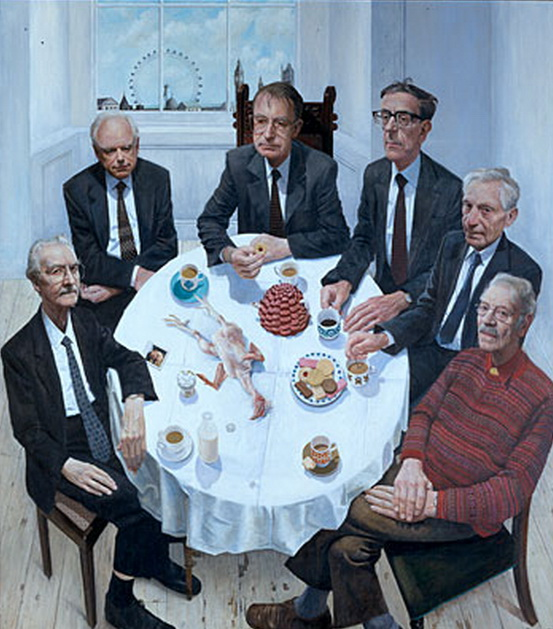
\includegraphics[width=\dimexpr(\textwidth+150pt)]{stuartpearson}}%
         \end{picture}%
      }%
    \let\@oddhead\@evenhead%
    \let\@mkboth\@gobbletwo%
    \let\chaptermark\@gobble%
    \let\sectionmark\@gobble%
 }


\def\doubletakeimage{%
  \renewcommand{\topfraction}{.95}  % ensure seecond image will not float away
  \begin{figure}[t]
    \thispagestyle{caption}
    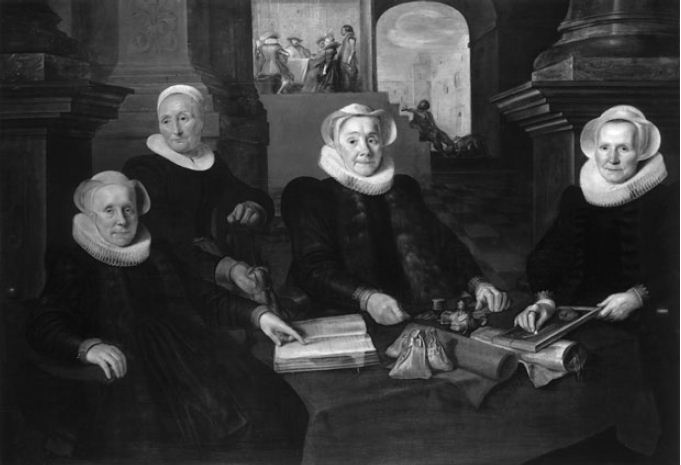
\includegraphics[width=\textwidth]{matron}%
  \end{figure}

  \begin{figure}[tp]
   \hspace*{-\marginparwidth}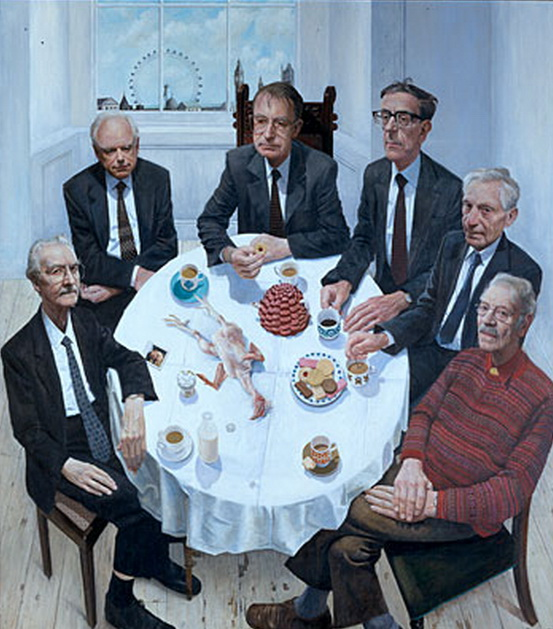
\includegraphics[height=0.9\textheight]{stuartpearson}
 \end{figure}
}


\doubletakeimage
\lipsum[1-4]
\begin{figure}[htp]
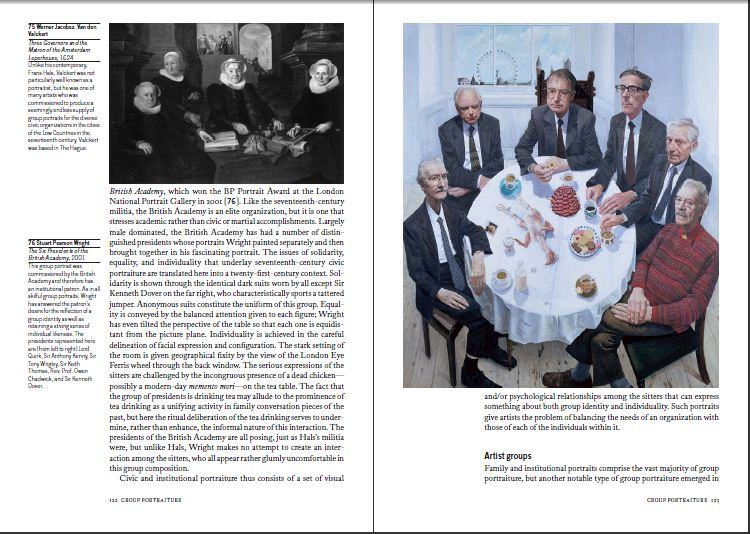
\includegraphics[width=0.98\textwidth]{captionspecial}
\centering
\caption{Figure from \textit{Oxford History of Art, Portraiture}, Shearer West, Oxford University Press, 2004. The figures are numbered consecutively and the text in the List of Illustrations have different formatting.}
\end{figure}
\restoregeometry
%% RESET EVERYTHING AT END OF CHAPTER
\addtocounter{chapter}{-2}
\@toctrue\@specialtrue

%\@specialfalse
\cxset{manet, toc image=false}
\cxset{toc image=false},
\topimage{manet}

\chapter{THE BARMAID}
\begin{multicols}{3}
      \leftskip0pt
      \lettrine{I}{psum dolor} sit amet latixeus. \lipsum*[1-2]
      Latinicus porcupinus to fill the line.
      \tikz{\draw[thick] (0,0)--(\columnwidth,0);}
\end{multicols}
\clearpage


%\cxset{manet, toc image=false}
%\cxset{toc image=false},
%\topimage{Alan-MacDonald-Cardinal-Spin-01}
%\chapter{THE BARMAID}
%\begin{multicols}{3}
%      \leftskip0pt
%      \lettrine{I}{psum dolor} sit amet latixeus. \lipsum*[1-2]
%      Latinicus porcupinus to fill the line.
%\end{multicols}
%\clearpage
%\@specialfalse
\cxset{manet,toc image=false}
\topimage{Alan-MacDonald-Cardinal-Spin-01}

\chapter{A New Approach to Designing \LaTeX\ Classes}
\begin{multicols}{3}
      \leftskip0pt
      \lettrine{I}{psum dolor} sit amet latixeus. \lipsum*[1-2]
      Latinicus porcupinus to fill the line.
\end{multicols}
\clearpage



This particular code, uses the predefined style \textit{manet}. The only difference we have now defined a helper macro to make it easier for such images to be inserted for similar style chapter openings.

\medskip

\begin{lstlisting}
\def\topimage#1{\cxset{title before={\hskip-2.3cm\includegraphics[width=1.25\textwidth]{./chapters/#1}\par
\vspace*{\baselineskip}\par}}}
\end{lstlisting}

If a full book is to be designed using chapter openings in this fashion more keys and styles could be defined to make it even more easy to enter.

The full code to have the chapter typeset is shown below:
\medskip

\begin{lstlisting}
\cxset{manet}
\topimage{Alan-MacDonald-Cardinal-Spin-01}

\chapter{ALAN MacDONALD}
\begin{multicols}{3}
      \leftskip0pt
      \lettrine{I}{psum dolor} sit amet latixeus. \lipsum*[1-2]
      Latinicus porcupinus to fill the line.
\end{multicols}
\end{lstlisting}
\lipsum[2]





%\cxset{toc image=false},
%% STYLE PICTURE IN OPENING PAGE
\long\gdef\versochapter#1{%
  \vspace*{3cm}
  \minipage{\textwidth}
  \hfill\includegraphics[width=0.63\textwidth]{\chapterimage@cx}\par
  \vspace*{6pt}
  \hfill\minipage{0.75\textwidth}
  {\HUGE\bfseries\flushright #1\endflushright}
  \endminipage
  \endminipage
  \newpage

% for recto page
\vspace*{10cm}
\@specialfalse
\@openleftfalse
\@openanyfalse
\@openrighttrue
}
%customedesign@cx

\newgeometry{bottom=2.5cm}

\cxset{
   chapter image/.code={\def\chapterimage@cx{#1}},
   chapter opening/.is choice,
   chapter opening/verso/.code={\@specialtrue\@openlefttrue
   \gdef\customdesign@cx##1{\versochapter{##1}}}
}

\cxset{
 chapter image=onesowndeath,
 chapter opening=verso,
 name={},
 numbering=none,
 number font-size=\LARGE,
 number font-family=\rmfamily,
 number font-weight=\bfseries,
 number before=,
 number dot=,
 number after=,
 number position=leftname,
 chapter font-family=\sffamily,
 chapter font-weight=\normalfont,
 chapter font-size=\Large,
 chapter before={\vspace*{0pt}\par},
 chapter after={\hfill\hfill\par},
 chapter color={black!90},
 number color=\color{purple},
 title beforeskip={\vspace*{0pt}},
 title afterskip={\vspace*{0.4\textheight}\par},
 title before={},
 title after={},
 title font-family=\sffamily,
 title font-color=\color{purple},
 title font-weight=\bfseries,
 title font-size=\LARGE,
 header style=plain,
 pagestyle=plain,
 }

\@specialtrue

\chapter[VERSO CHAPTERS]{Verso Chapters}

\parindent1.5em
{\HUGE V}erso chapter openings are not common. One design that I found quite attractive is \lipsum[1-3] \textit{From Western attitudes toward death from the middle ages to the present}, Philippe Ari\'es. London, 1974.

\begin{figure}
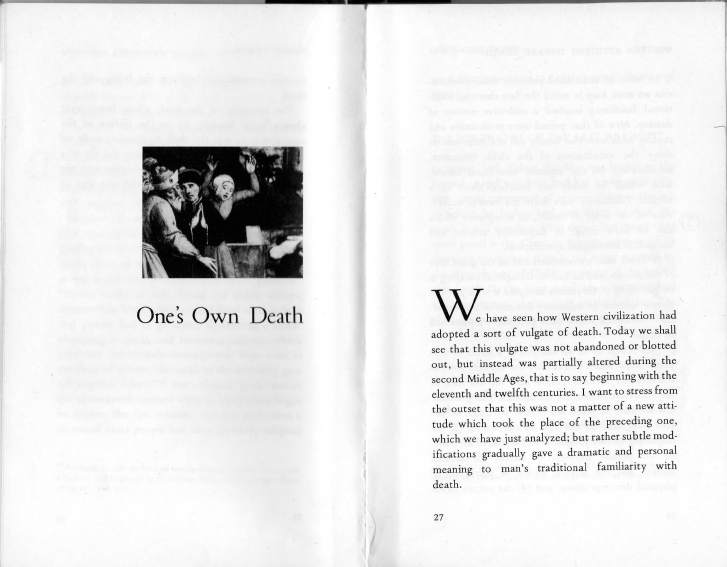
\includegraphics[width=\textwidth]{versochapter01}
\caption{Chapter opening on verso page.}
\end{figure}


%\@specialfalse
%%%%%%%%%%%%%%%%%%%%%%%%%%%%%%%%%%%%%%%%%%%
%%%%%%  STYLE 01
%%%%%%%%%%%%%%%%%%%%%%%%%%%%%%%%%%%%%%%%%%%


\cxset{
 name={},
 numbering=arabic,
 number font-size=\LARGE,
 number font-family=\rmfamily,
 number font-weight=\bfseries,
 number before=,
 number dot=,
 number after=,
 number position=leftname,
 chapter font-family=\sffamily,
 chapter font-weight=\normalfont,
 chapter font-size=\Large,
 chapter before={\vspace*{20pt}\par},
 chapter after={\hfill\hfill\par},
 chapter color={black!90},
 number color=\color{purple},
 title beforeskip={\vspace*{30pt}},
 title afterskip={\vspace*{40pt}\par},
 title before={},
 title after={},
 title font-family=\sffamily,
 title font-color=\color{purple},
 title font-weight=\bfseries,
 title font-size=\LARGE,
 header style=headings}

\cxset{headings ruled-01}

\chapter{Introduction to Style One}


\begin{summary}
This design is simple and its distinguishing characteristic is a short summary at the beginning of the chapter. This is almost like an abstract typeset in italic font without setting the margins in. We provide a \lstinline{summary} environment for convenience. Note the very simple line in the running head to the left of the page number.
\end{summary}

\medskip
\begin{figure}[ht]
\centering
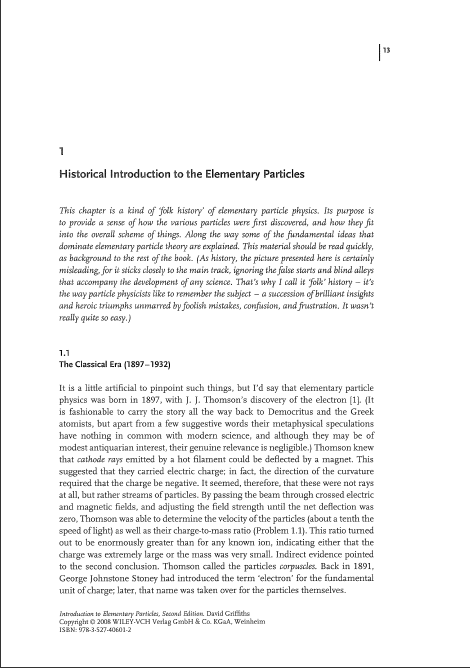
\includegraphics[width=0.5\textwidth]{./chapters/chapter01}
\end{figure}


%
%%%%%%%%%%%%%%%%%%%%%%%%%%%%%%%%%%%%%%%%%%%
%%%%%%  STYLE 02
%%%%%%%%%%%%%%%%%%%%%%%%%%%%%%%%%%%%%%%%%%%
\clearpage

\cxset{
 name={},
 numbering=arabic,
 number font-size=\LARGE,
 number font-family=\rmfamily,
 number font-weight=\bfseries,
 number before=,
 number dot=.,
 number after=\hspace{1em},
 number position=rightname,
 chapter font-family=\sffamily,
 chapter font-weight=\normalfont,
 chapter font-size=\Large,
 chapter before={\vspace*{20pt}\par\hfill},
 chapter after={},
 chapter color={black!90},
 number color=\color{purple},
 title beforeskip={},
 title afterskip={\vspace*{50pt}\par},
 title before={},
 title after={},
 title font-family=\sffamily,
 title font-color=\color{purple},
 title font-weight=\bfseries,
 title font-size=\LARGE}

\chapter{Style 2}
\parindent0pt
I tend to favour this design for books that have a lot of pictures. It brings the design into the margins and leaves plentiful white space in the margins. From a programming point of view the chapter is the opposite of openany. It has to open on an odd number.
\medskip
\begin{figure}[ht]
\centering
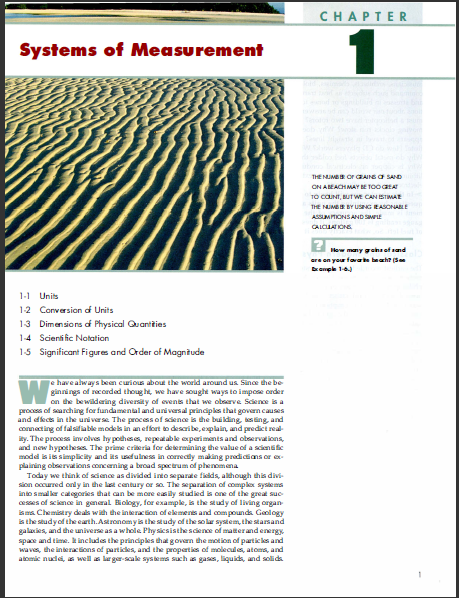
\includegraphics[width=0.6\textwidth]{./chapters/chapter02}
\end{figure}


%%%%%%%%%%%%%%%%%%%%%%%%%%%%%%%%%%%%%%%%%%%%
%%%%%%  STYLE 03
%%%%%%%%%%%%%%%%%%%%%%%%%%%%%%%%%%%%%%%%%%%
\newgeometry{top=-10pt,bottom=2cm}
\tcbset{width=\paperwidth,boxrule=0pt,right=3cm,arc=0pt}

\cxset{style03/.style={
 name={},
 numbering=arabic,
 number font-size=\HUGE,
 number font-family=\rmfamily,
 number font-weight=\bfseries,
 number before=,
 number dot=.,
 number after=,
 number position=rightname,
 chapter font-family=\sffamily,
 chapter font-weight=\normalfont,
 chapter font-size=\Large,
% start colorbox
 chapter before={\hspace*{-2.5cm}\vbox\bgroup\tcolorbox\bgroup\vspace*{20pt}\hfill\hfill},
 chapter after={\par\vspace*{15pt}},
 chapter color={black!90},
 number color=\color{purple},
 title beforeskip={},
 title afterskip={\vspace*{10pt}\par},
 title before={\hfill\hfill},
% end colorbox
 title after={\vspace*{60pt}\egroup\endtcolorbox\egroup},
 title font-family=\sffamily,
 title font-color=\color{purple},
 title font-weight=\bfseries,
 title font-size=\Huge}}

\cxset{style03}

\chapter{Introduction Style Three}

This is not an exact reproduction as I am still thinking as to how to use
specials with the package. You can vary it by setting the tcolorbox settings as well as the geometry settings.
\medskip
\begin{figure}[ht]
\centering
\includegraphics[width=0.39\textwidth]{./chapters/chapter03}
\end{figure}

This setting involves changing the geometry of the page as well as adding the chapter name and title in a color box. For this I have used the \lstinline{tcolorbox}. Of course you can use any other shaded environment you feel comfortable with such as mdframed. It is important to set the colorbox parameters.

\begin{lstlisting}
\newgeometry{top=-10pt}
\tcbset{width=\paperwidth,boxrule=0pt,right=3cm,arc=0pt}
\end{lstlisting}

Note that we set the width of the \lstinline{tcolorbox} to \lstinline{\paperwidth} in order for the shading to extend to the full width of the page.

\restoregeometry

%%%%%%%%%%%%%%%%%%%%%%%%%%%%%%%%%%%%%%%%%%%%
%%%%%%  STYLE 04
%%%%%%%%%%%%%%%%%%%%%%%%%%%%%%%%%%%%%%%%%%%
\clearpage
\cxset{style04/.style={
 name={},
 numbering=Roman,
 number font-size=\Large,
 number font-family=\rmfamily,
 number font-weight=\bfseries,
 number before=,
 number dot=,
 number after=,
 number position=rightname,
 chapter font-family=\rmfamily,
 chapter font-weight=\normalfont,
 chapter font-size=\Large,
 chapter before={\vspace*{20pt}\par\hfill},
 chapter after={\hfill\hfill\par\vspace*{10pt}},
 chapter color={black!90},
 number color=\color{purple},
 title beforeskip={},
 title afterskip={\vspace*{50pt}\par},
 title before={\hfill},
 title after={\hfill\hfill\par},
 title font-family=\rmfamily,
 title font-color=\color{purple},
 title font-weight=\normalfont,
 title font-size=\LARGE}}

\cxset{style04}

\chapter{INTRODUCTION TO STYLE FOUR}

This is a very simple design applicable perhaps to translations and commentary on older texts.
\medskip
\begin{figure}[ht]
\centering
\includegraphics[width=0.6\textwidth]{./chapters/chapter04}
\end{figure}

%%%%%%%%%%%%%%%%%%%%%%%%%%%%%%%%%%%%%%%%%%%%
%%%%%%  STYLE 05
%%%%%%%%%%%%%%%%%%%%%%%%%%%%%%%%%%%%%%%%%%%


\cxset{style05/.style={
 name={Chapter},
 numbering=arabic,
 number font-size=\Large,
 number font-family=\rmfamily,
 number font-weight=\normalfont\itshape,
 number color=\color{black!90},
 number before=,
 number dot=,
 number after=,
 number position=rightname,
 chapter font-family=\rmfamily,
 chapter font-weight=\normalfont\itshape,
 chapter font-size=\Large,
 chapter before={\hrule width \columnwidth \kern2.6\p@ \par\hfill},
 chapter after={\hfill\hfill\par},
 chapter color={black!90},
 chapter spaceout=none,
 title beforeskip={\vspace*{10pt}},
 title afterskip={\vspace*{50pt}\par},
 title before={\hfill},
 title after={\hfill\hfill \vskip2.6pt\hrule width \columnwidth \kern2.6\p@ },
 title font-family=\rmfamily,
 title font-color=\color{black!90},
 title font-weight=\bfseries,
 title font-size=\huge,
 header style=empty}}

\cxset{style05}
\chapter{Introduction to Style Five}\index{ch:style5}

\tcbset{width=\textwidth}
I think this style can be improved with a bit of color. You can experiment with it quite easily. The spacing on top of this style can also be adjusted to suit your typographical taste.
\medskip
\begin{figure}[ht]
\centering
\includegraphics[width=0.6\textwidth]{./chapters/chapter05}
\end{figure}

\section{General notes on rules}

LaTeX's default rules would normally give problems. Best is to use TeX's primitives to built them.

\index{rules!example color}
\begin{texexample}{}{}
\hrule width 5cm \kern2.6\p@
AAAAAAAAAAAAAAAAAAAAA
\vskip2.6pt\hrule width 5cm
\medskip

Problem with LaTeX rules.

\rule{5cm}{0.4pt}\par
AAAAAAAAAAAAAAAAAAAAA\par%
\rule[6.5pt]{5cm}{0.4pt}

\def\rule{\@ifnextchar[\@rule{\@rule[\z@]}}
\def\@rule[#1]#2#3{%
 \leavevmode
 \hbox{%
 \setlength\@tempdima{#1}%
 \setlength\@tempdimb{#2}%
 \setlength\@tempdimc{#3}%
 \advance\@tempdimc\@tempdima%
 \vrule\@width\@tempdimb\@height\@tempdimc\@depth-\@tempdima}}

\def\thickrule{\leavevmode \leaders \hrule height 3pt \hfill \kern \z@}

{\color{teal}\hrule width 10.5cm height3pt \kern2.6\p@
    {{\color{black!80}\HUGE CHAPTER TITLE}}\vskip3pt
\hrule width 10.5cm height3pt}
\end{texexample}

%%%%%%%%%%%%%%%%%%%%%%%%%%%%%%%%%%%%%%%%%%%%
%%%%%%  STYLE 06
%%%%%%%%%%%%%%%%%%%%%%%%%%%%%%%%%%%%%%%%%%%

\cxset{style06/.style={
 name={Chapter},
 numbering=arabic,
 number font-size=\Huge,
 number font-family=\calligra,
 number font-weight=\calligra,
 number color=\color{black!90},
 number before=\kern-2.5pt,
 number dot=,
 number after=,
 number position=rightname,
 chapter font-family=\rmfamily,
 chapter font-weight=\calligra,
 chapter font-size=\LARGE\calligra,
 chapter before={\vspace*{20pt}\par\hfill},
 chapter after={\hfill\hfill\par},
 chapter color={black!90},
 title beforeskip={\vspace*{50pt}},
 title afterskip={\vspace{3.5pt}\par},
 title before={\hfill},
 title after={\hfill\hfill},
 title font-family=\rmfamily,
 title font-color=\color{black!90},
 title font-weight=\normalfont,
 title font-size=\LARGE,
 title spaceout=soul,
}}

\cxset{style06}

\chapter{INTRODUCTION TO STYLE SIX}
\renewcommand{\DefaultLhang}{0.1}
\renewcommand{\LettrineFontHook}{\calligra}
\setlength{\DefaultFindent}{9.5pt}
\setlength{\DefaultNindent}{0pt}

\lettrine{\textcolor{orange}{T}}{}he calligraphic font for this design make it stand out, although you may need to experiment to get the right font (I have used calligra). I am sure the specification can be optimized a bit, however so far it works. I also opted to space out the title. I had to experiment a bit to get the Lettrine settings.
\medskip
\begin{figure}[ht]
\centering
\includegraphics[width=0.6\textwidth]{./chapters/chapter06}
\end{figure}

The number has been kerned using:

\begin{lstlisting}
 number before=\kern-4.5pt,
\end{lstlisting}

This template has a lot of potential and I will come back to it and add more key hooks for lettrine settings per letter and font management. They can also come alive with a gold color.


%
\newgeometry{top=2cm,bottom=2cm,left=3cm,right=3cm}
%%%%%%%%%%%%%%%%%%%%%%%%%%%%%%%%%%%%%%%%%%%
%%%%%%  STYLE 07
%%%%%%%%%%%%%%%%%%%%%%%%%%%%%%%%%%%%%%%%%%%

\cxset{style07/.style={
 name={},
 numbering=arabic,
 number font-size=\Huge,
 number font-family=\rmfamily,
 number font-weight=\bfseries,
 number before=,
 number dot=,
 number color=\color{gray},
 number after=\par,
 number position=rightname,
 chapter font-family=\sffamily,
 chapter font-weight=\normalfont,
 chapter font-size=\Large,
 chapter before={\hfill\hfill\par},
 chapter after={},
 chapter color={black!90},
 title beforeskip={\vspace*{30pt}},
 title afterskip={\vspace*{50pt}\par},
 title before={},
 title after={\par\rule[13pt]{\textwidth}{0.4pt}},
 title font-family=\sffamily,
 title font-color=\color{purple},
 title font-weight=\bfseries,
 title font-size=\LARGE,
 title spaceout=none,
}}

\cxset{style07}
\chapter{Introduction to Style Seven}

\parindent0pt
\lipsum[1]
\medskip
\begin{figure}[ht]
\centering
\includegraphics[width=0.6\textwidth]{./chapters/chapter07}
\end{figure}
\lipsum[1]

%%%%%%%%%%%%%%%%%%%%%%%%%%%%%%%%%%%%%%%%%%%%
%%%%%%  STYLE 08
%%%%%%%%%%%%%%%%%%%%%%%%%%%%%%%%%%%%%%%%%%%
\clearpage

\cxset{style08/.style={
 name={},
 numbering=arabic,
 number font-size=\LARGE,
 number font-family=\sffamily,
 number font-weight=\bfseries,
 number color=\color{black!90},
 number before=,
 number dot=,
 number after=,
 number position=rightname,
 chapter font-family=\sffamily,
 chapter font-weight=\normalfont,
 chapter font-size=\Large,
 chapter before={\vspace*{20pt}\hfill},
 chapter after={\vspace{20pt}\par},
 chapter color={black!90},
 title beforeskip={},
 title afterskip={\vspace*{50pt}\par},
 title before={\hfill\hfill\raggedleft},
 title after={},
 title font-family=\sffamily,
 title font-color=\color{black!90},
 title font-weight=\bfseries,
 title font-size=\LARGE,
 author block=true,
 author block format=\par\addvspace{12pt}\normalfont\large\raggedleft,
 author names=Yiannis Lazarides\par Larnaka,
 header style=empty}}

\cxset{style08}
\chapter{Introduction to Chapter Style Eight}

\lipsum[1]
\medskip
\begin{figure}[ht]
\centering
\includegraphics[width=0.5\textwidth]{./chapters/chapter08}
\end{figure}
\lipsum[1]

%\cxset{author block=false}
%%%%%%%%%%%%%%%%%%%%%%%%%%%%%%%%%%%%%%%%%%%
%%%%%%  STYLE 09
%%%%%%%%%%%%%%%%%%%%%%%%%%%%%%%%%%%%%%%%%%%
\clearpage

\cxset{
 name={},
 numbering=arabic,
 number font-size=\LARGE,
 number font-family=\rmfamily,
 number font-weight=\bfseries,
 number before=,
 number dot=.,
 number after=\hspace{1em},
 number position=rightname,
 chapter font-family=\sffamily,
 chapter font-weight=\normalfont,
 chapter font-size=\Large,
 chapter before={\vspace*{20pt}\par\hfill},
 chapter after={},
 chapter color={black!90},
 number color=\color{purple},
 title beforeskip={},
 title afterskip={\vspace*{50pt}\par},
 title before={},
 title after={},
 title font-family=\sffamily,
 title font-color=\color{purple},
 title font-weight=\bfseries,
 title font-size=\LARGE}
\chapter{Introduction 09}
\lipsum[1]

\medskip
\begin{figure}[ht]
\centering
\includegraphics[width=0.8\textwidth]{./chapters/chapter09}
\end{figure}

\textit{In preparation. Patience!}

%%%%%%%%%%%%%%%%%%%%%%%%%%%%%%%%%%%%%%%%%%%%
%%%%%%  STYLE 10
%%%%%%%%%%%%%%%%%%%%%%%%%%%%%%%%%%%%%%%%%%%

\cxset{
 name=CHAPTER,
 numbering=WORDS,
 number font-size=\huge,
 number font-family=\sffamily,
 number font-weight=\bfseries,
 number before=,
 number dot=,
 number after=\hspace{1em},
 number position=rightname,
 chapter font-family=\sffamily,
 chapter font-weight=\bfseries,
 chapter font-size=\huge,
 chapter before={\vspace*{0.4\textheight}\hfill},
 chapter after={\hfill\hfill\vskip0pt\thinrule\par},
 chapter color={black!90},
 number color=\color{black!90},
 title beforeskip={\vspace*{30pt}},
 title afterskip={\vspace*{30pt}\par},
 title before={\hfill},
 title after={\hfill\hfill},
 title font-family=\sffamily,
 title font-color=\color{black!90},
 title font-weight=\bfseries,
 title font-size=\huge,
 section font-size=\LARGE,
 section font-weight=\normalfont,
 section font-family=\sffamily,
 section align=,
 section numbering=none,
 section indent=-1em,
 section align=\centering,
 section beforeskip=20pt,
 section afterskip=10pt,
 section spaceout=soul,
 section font-shape=,
}

 %set the sectioning commands


\renewsection

\chapter{INTRODUCTION TO STYLE TEN}

\section{Basic Description:}
This chapter style has the unique characteristic that the chapter number is spelled out, rather than being in arabic numerals. The setting for this is the option \lstinline{numeric=WORDS}. Use either a capital for uppercase or \lstinline{numeric=words} for lowercase number labels.

\medskip
\begin{figure}[ht]
\centering
\includegraphics[width=0.6\textwidth]{./chapters/chapter10}
\end{figure}

\lipsum[1]

%%%%%%%%%%%%%%%%%%%%%%%%%%%%%%%%%%%%%%%%%%%%
%%%%%%  STYLE 11
%%%%%%%%%%%%%%%%%%%%%%%%%%%%%%%%%%%%%%%%%%%

\cxset{style11/.style={
 name={Chapter},
 numbering=arabic,
 number font-size=\LARGE,
 number font-family=\rmfamily,
 number font-weight=\bfseries,
 number before=,
 number dot=,
 number after=,
 number position=rightname,
 chapter font-family=\rmfamily,
 chapter font-weight=\bfseries,
 chapter font-size=\LARGE,
 chapter before={\vspace*{20pt}\par\hfill},
 chapter after={\hfill\hfill\par\vspace{10pt}},
 chapter color={black!90},
 number color=\color{black!90},
 title beforeskip={},
 title afterskip={\vspace*{20pt}\par},
 title before={\hfill},
 title after={\hfill\hfill\par},
 title font-family=\rmfamily,
 title font-color=\color{black!90},
 title font-weight=\bfseries,
 title font-size=\LARGE}}

\cxset{style11}
\chapter{Introduction to Style Eleven}
\lipsum[2]

\medskip
\begin{figure}[ht]
\centering
\fbox{\includegraphics[width=0.65\textwidth]{./chapters/chapter11}}
\end{figure}
\lipsum[1]

%%%%%%%%%%%%%%%%%%%%%%%%%%%%%%%%%%%%%%%%%%%%
%%%%%%  STYLE 12
%%%%%%%%%%%%%%%%%%%%%%%%%%%%%%%%%%%%%%%%%%%
\cxset{style12/.style={
 name={},
 numbering=arabic,
 number font-size=\HUGE,
 number font-family=\rmfamily,
 number font-weight=\bfseries,
 number before=,
 number dot=,
 number color=\color{gray},
 number after=\par,
 number position=rightname,
 chapter font-family=\sffamily,
 chapter font-weight=\normalfont,
 chapter font-size=\Huge,
 chapter before={\raggedright\par},
 chapter after={},
 chapter color={black!90},
 title beforeskip={\vspace*{30pt}},
 title afterskip={\vspace*{50pt}\par},
 title before={},
 title after={\par\vspace{30pt}\rule{\textwidth}{4pt}},
 title font-family=\sffamily,
 title font-color=\color{purple},
 title font-weight=\bfseries,
 title font-size=\HUGE,
 title spaceout=none,
}}


\cxset{style12}
\chapter{Introduction to \\ Style Twelve}

This is a variation of Style 7, with only the lettering and the rule are thicker. In my opinion it looks better with a bit of color, so I have used a purple color with a gray.

\medskip
\begin{figure}[ht]
\centering
\includegraphics[width=0.35\textwidth]{./chapters/chapter12}
\end{figure}
\lipsum[1]

%%%%%%%%%%%%%%%%%%%%%%%%%%%%%%%%%%%%%%%%%%%%
%%%%%%  STYLE 13
%%%%%%%%%%%%%%%%%%%%%%%%%%%%%%%%%%%%%%%%%%%

\cxset{style13/.style={
 name={Chapter},
 numbering=arabic,
 number font-size=\HUGE,
 number font-family=\sffamily,
 number font-weight=\bfseries,
 number color=\color{gray!50},
 number before=\par\vspace*{5pt}\hfill\hfill,
 number dot=,
 number after={\hspace*{7pt}\par},
 number position=rightname,
 chapter font-family=\sffamily,
 chapter font-weight=\normalfont,
 chapter font-size=\LARGE,
 chapter before={\thickrule\vspace*{20pt}\par\hfill\hfill},
 chapter after={\vskip0pt\par},
 chapter color={black!50},
 title beforeskip={\vspace*{10pt}},
 title afterskip={\vspace*{50pt}\par},
 title before={\hfill\hfill\raggedleft},
 title after={},
 title font-family=\sffamily,
 title font-color=\color{thered},
 title font-weight=\bfseries,
 title font-size=\huge,
 section indent=-1em,
 section align=\raggedright,
 section numbering=arabic,
 section indent=0pt,
 section beforeskip=0pt,
 section afterskip=\baselineskip,
 subsection align=\raggedright,
 subsection font-family=\sffamily,
 subsection font-weight=\bfseries,
 subsection font-size=\large,
 subsection font-shape=\itshape,
 subparagraph number after=\space,
}
}

\def\setstyle#1{\cxset{style#1}%
 \renewsection\renewsubsection\renewsubsubsection%
 \renewparagraph\renewsubparagraph}

\setstyle{13}


\chapter{Introduction to Chapter\\ Style Thirteen}

\section{A Brief History of Biomedical\\ Fluid Mechanics}
\lorem
\medskip
\begin{figure}[ht]
\centering
\includegraphics[width=0.45\textwidth]{./chapters/chapter14}
\includegraphics[width=0.45\textwidth]{./chapters/chapter14a}
\end{figure}
\lorem
 % CHECK FOR ERRORS
%%%%%%%%%%%%%%%%%%%%%%%%%%%%%%%%%%%%%%%%%%%%
%%%%%%  STYLE 14
%%%%%%%%%%%%%%%%%%%%%%%%%%%%%%%%%%%%%%%%%%%
\clearpage

\cxset{
 name={},
 numbering=arabic,
 number font-size=\LARGE,
 number font-family=\rmfamily,
 number font-weight=\bfseries,
 number before=,
 number dot=.,
 number after=\hspace{1em},
 number position=rightname,
 chapter font-family=\sffamily,
 chapter font-weight=\normalfont,
 chapter font-size=\Large,
 chapter before={\vspace*{20pt}\par\hfill},
 chapter after={},
 chapter color={black!90},
 number color=\color{purple},
 title beforeskip={},
 title afterskip={\vspace*{50pt}\par},
 title before={},
 title after={},
 title font-family=\sffamily,
 title font-color=\color{purple},
 title font-weight=\bfseries,
 title font-size=\LARGE}
\chapter{Introduction 14}
\lipsum[1]
\medskip
\begin{figure}[ht]
\centering
\includegraphics[width=0.65\textwidth]{./chapters/chapter14}
\end{figure}
\lipsum[2]

%%%%%%%%%%%%%%%%%%%%%%%%%%%%%%%%%%%%%%%%%%%%
%%%%%%  STYLE 15
%%%%%%%%%%%%%%%%%%%%%%%%%%%%%%%%%%%%%%%%%%%
\newgeometry{left=2cm,right=7cm, marginparsep=15pt, marginparwidth=4.2cm,top=2cm}
\cxset{
 name={},
 numbering=none,
 number font-size=\LARGE,
 number font-family=\rmfamily,
 number font-weight=\bfseries,
 number before=,
 number dot=,
 number after=,
 number position=rightname,
 chapter font-family=\sffamily,
 chapter font-weight=\normalfont,
 chapter font-size=\Large,
 chapter before={},
 chapter after={},
 chapter color={black!90},
 number color=\color{purple},
 title beforeskip={},
 title afterskip={\vspace*{50pt}\par},
 title before={},
 title after={},
 title font-family=\rmfamily,
 title font-color=\color{black!80},
 title font-weight=\normalfont,
 title font-size=\Huge,
 title font-shape=\itshape,
 chapter opening=any,
 watermark text=SAMPLE PAGE,
 header style=samplepage}


\chapter{Introduction to Style Fifteen}

\parindent1em
\def\thefigure{\arabic{chapter}.\arabic{figure}}
\lorem\par

\marginpar{%
 {\centering
 \includegraphics[width=4.2cm]{./chapters/chapter15}\vskip5pt\par}
 {\footnotesize\lorem}
}
\marginpar{%
{\centering
\includegraphics[width=4.2cm]{./chapters/chapter15}\par}
 { \captionof{figure}{\footnotesize\lorem}}
}
This is another marginpar of the same size.

\lorem

\lipsum
\marginpar{%
{\centering
\includegraphics[width=4.2cm]{./chapters/chapter15}\par}
 { \captionof{figure}{\footnotesize\lorem}}
}
%%%% END STYLE %%%%%%%%%%%%%%%%%%%%%%%%%%%%%%%%%

%
\newgeometry{left=7.5cm,right=2cm, marginparsep=15pt, marginparwidth=4.2cm,top=2cm}
%%%%%%%%%%%%%%%%%%%%%%%%%%%%%%%%%%%%%%%%%%%
%%%%%%  STYLE 16
%%%%%%%%%%%%%%%%%%%%%%%%%%%%%%%%%%%%%%%%%%%


\cxset{style16/.style={
 chapter opening=anywhere,
 name={},
 numbering=arabic,
 number color=\color{thegray},
 number font-size=\HHUGE,
 number font-family=\rmfamily,
 number font-weight=\bfseries,
 number before=\leftskip-4cm\vbox to 0cm\bgroup\vspace*{5cm},
 number after=\egroup\vskip0pt\par,
 number dot=,
 number position=leftname,
 chapter font-family=\sffamily,
 chapter font-weight=\normalfont,
 chapter font-size=\Large,
 chapter before={},
 chapter after={\begin{picture}(0,0)
                          \put(-50pt,\dimexpr-\textheight+\footskip+20pt\relax){\parbox{\marginparwidth}{\textbf{Napoleon}\par
Some long caption typeset in a parbox of width marginparwidth \lorem}}%
                        \end{picture}},
 chapter color={black!90},
 title beforeskip={\par\hspace*{4cm}\thinrule\vskip0pt\hspace*{4cm}\vbox\bgroup},
 title afterskip={\vspace*{50pt}\par\egroup},
 title before={},
 title after=,
 title font-color=\color{black!80},
 title font-weight=\normalfont,
 title font-family=\rmfamily,
 title font-shape=\upshape,
 title font-size=\HUGE,
 header style=empty,
 subsection numbering=none,
 subsection color=teal,
 subsection align=\color{teal},
 }}

\renewsubsection

%%%% VERSO NAPOLEON %%%%%%%%%%%
% We define a macro to set the page dimensions to full.
% We also require the parindent to be set to 0pt and to restore it afterwards.
\def\fullpageimage{%
       \vspace*{-2.5cm}
        \parindent0pt
       \hspace*{-2cm}\includegraphics[width=\paperwidth]{napoleon}%
  }}


\cleardoublepage
\fullpageimage

\cxset{style16}
\chapter{Victorian England:\\ Introduction 16}
\label{style16}
This design from a Social Sciences book had to be set into two vboxes and negative skips allowed to line
up the numbers. Once I am totally happy with it, I will add parameter adjustments, as well as a bit of automation of length calculations.

\medskip

\begin{figure}[ht]
\centering
\includegraphics[width=0.35\textwidth]{./chapters/chapter16}
\end{figure}
\lipsum[2]

\cxset{geometry marginparsep/.code=\setlength\marginparsep{#1},
          geometry marginparwidth/.code=\setlength{\marginparwidth}{#1}}

\section{Technical notes}

This design looks simple but takes a bit of effort to achieve it, especially due to the tendency of LaTeX and the TeX engine to make decisions for you. Firstly we cannot reset the page geometry between the image and the chapter, as this will either result in unpredictable behaviour or if you use the \cs{newgeometry} macro, it will for certain leave a blank page in between.

\begin{description}
\item [image sizing] The image is set at \textbf{width=paperwidth}. This can vary depending on the page geometry and the image aspect ratio. In general you may need to ensure that your image has the same aspect ratio as the page to avoid problems with placement and the generation of extra blank pages.
\item [image caption] The image caption is placed using the picture environment, so that it can be typeset absolutely, feel free to use TikZ for the same purpose. We also use Heiko Oberdiek's the \pkg{picture} package to make calculations easier by specifying actual dimensions and not needing to strip the point.
\end{description}

% Best to always restore geometry after you have changed it.

\restoregeometry


%%%%%%%%%%%%%%%%%%%%%%%%%%%%%%%%%%%%%%%%%%%%
%%%%%%  STYLE 17
%%%%%%%%%%%%%%%%%%%%%%%%%%%%%%%%%%%%%%%%%%%
\newgeometry{left=7cm,right=2cm, marginparsep=15pt, marginparwidth=4.2cm,top=2cm,%
reversemarginpar}
\cxset{style17/.style={
 name={},
 numbering=arabic,
 number font-size=\huge,
 number font-family=\sffamily,
 number font-weight=\bfseries,
 number before=,
 number dot=.,
 number color=\color{purple},
 number after=\thinspace,
 number position=rightname,
 chapter font-family=\sffamily,
 chapter font-weight=\bfseries,
 chapter font-size=\LARGE,
 chapter before={\vspace*{20pt}\par\hfill},
 chapter after={},
 chapter color={black!90},
 title beforeskip={},
 title afterskip={\vspace*{70pt}\par},
 title before={},
 title after={},
 title font-family=\sffamily,
 title font-color=\color{purple},
 title font-shape=\upshape,
 title font-weight=\bfseries,
 title font-size=\huge,
 section numbering=none,
 section beforeskip=10pt,
 section afterskip=10pt,
 section font-family=\rmfamily,
 section font-shape=\slshape,
 geometry marginparwidth=4.5cm,
 geometry marginparsep=20pt}}
\cxset{style17}

\chapter{Introduction to Style Seventeen}

I tend to favour this design for books that have a lot of pictures. It brings the design into the margins and leaves plentiful white space in the margins. From a programming point of view the chapter is the opposite of openany. It has to open on an odd number.

\marginpar{%
\vspace*{0.2\textheight}
\includegraphics[width=\marginparwidth]{./chapters/chapter17}\par
{\footnotesize\lorem}
}

\section{Use the margins}

Adjustments to the geometry layout can be carried out temporarily or permanently via the use of keys and
the geometry package. These are probably the less problematic and easier to set geometry settings.

\section{Margin notes}

Marginal notes use the same mechanism as
floats to communicate with the \cs{output} routine. Marginal notes are distinguished from
floats by having a negative placement specification. The command
\cs{marginpar}\oarg{left text}\marg{right text} generates a marginal note in a parbox,
using LTEXT if it's on the left and RTEXT if it's on the right.
(Default is RTEXT = LTEXT.) It uses the following parameters.
\cs{marginparwidth}: Width of marginal notes.
\cs{marginparsep}: Distance between marginal note and text.
the page layout to determine how to move the marginal
note into the margin. E.g.,

\begin{tcolorbox}
\begin{lstlisting}
\@leftmarginskip ==\hskip -\marginparwidth \hskip -\marginparsep .
\end{lstlisting}
\end{tcolorbox}

\cs{marginparpush} Minimum vertical separation between \cs{marginpar}'s
Marginal notes are normally put on the outside of the page
if @mparswitch = true, and on the right if @mparswitch = false.
The command \cs{reversemarginpar} reverses the side where they
are put. \cs{normalmarginpar} undoes \cs{reversemarginpar}.
These commands have no effect for two-column output.
\marginpar{\footnotesize \textsc{\bfseries NOTE:} if two marginal notes appear on the same line of
text, then the second one could appear on the next page, in
a funny position.}
\section{Sample text}
\lipsum[2-4]

\restoregeometry

%%%%%%%%%%%%%%%%%%%%%%%%%%%%%%%%%%%%%%%%%%%%
%%%%%%  STYLE 18
%%%%%%%%%%%%%%%%%%%%%%%%%%%%%%%%%%%%%%%%%%%

\cxset{
 name={},
 numbering=arabic,
 number font-size=\Large,
 number font-family=\rmfamily,
 number font-weight=\normalfont,
 number before=,
 number after=\hspace{1em}\hfill\hfill\par\vspace*{20pt}\centerline{\textcolor{purple}{\decoone}}\vspace*{20pt},
 number dot=,
 number position=rightname,
% Chapter name settings
 name=CHAPTER,
 chapter font-family=\rmfamily,
 chapter font-weight=\normalfont,
 chapter font-size=\Large,
 chapter before={\vspace*{20pt}\par\hfill},
 chapter after={},
 chapter color={black!90},
 number color=\color{black!90},
 title beforeskip={},
 title afterskip={\vspace*{50pt}\par},
 title before={\hfill},
 title after={\hfill\hfill},
 title font-family=\rmfamily,
 title font-color=\color{black!90},
 title font-weight=\normalfont,
 title font-size=\Huge}
\chapter{Introduction to Chapter Style Eighteen}

\parindent0pt
This design introduces an ornament. There are a number of packages on ctan that provide ornaments. If you using XeLaTeX it is also possible to use system fonts. The ornament is introduced with the key number after. At this point also we introduced all the vertical skips.
\medskip
\begin{figure}[ht]
\centering
\includegraphics[width=0.45\textwidth]{./chapters/chapter18}
\end{figure}

%%%%%%%%%%%%%%%%%%%%%%%%%%%%%%%%%%%%%%%%%%%%
%%%%%%  STYLE 19
%%%%%%%%%%%%%%%%%%%%%%%%%%%%%%%%%%%%%%%%%%%
\cxset{style19/.style={
 name={},
 numbering=arabic,
 number font-size=\huge,
 number font-family=\rmfamily,
 number font-weight=\bfseries,
 number before=\par,
 number after=\hspace{1em},
 number dot={ },
 number position=rightname,
 chapter font-family=\rmfamily,
 chapter font-weight=\normalfont,
 chapter font-size=\huge,
 chapter before={\vspace*{20pt}},
 chapter after={},
 chapter color={black!90},
 number color=\color{black!90},
 title beforeskip={},
 title afterskip={\vspace*{50pt}\par},
 title before={\hangindent1.9em},
 title after={},
 title font-family=\sffamily,
 title font-color=\color{black!90},
 title font-weight=\bfseries,
 title font-size=\huge}}

\cxset{style19}
\chapter{Introduction to chapter\\ style nineteen}
\lipsum[1]

\medskip
\begin{figure}[ht]
\centering
\includegraphics[width=0.5\textwidth]{chapter19}
\end{figure}

\lipsum[1]

%\colorlet{toprule}{teal}
\colorlet{theblock}{teal}
%%%%%%%%%%%%%%
%%%%%%%%%%%%%%%%%%%%%%%%%%%%%
%%%%%%  STYLE 20
%%%%%%%%%%%%%%%%%%%%%%%%%%%%%%%%%%%%%%%%%%%
\cxset{rule color/.store in={\rulecolor@cx},
          block color/.store in={\blockcolor@cx}}
\cxset{style20/.style={
 rule color=teal!90,
 block color=teal!90,
 name={},
 numbering = arabic,
 number font-size=\HHUGE,
 number color=\color{white},
 number font-family=\sffamily,
 number font-weight=\bfseries,
 number before={\hbox to 0pt{\vbox to -10pt{\colorbox{\blockcolor@cx}{\rule{0pt}{70pt}\HHUGE \color{\blockcolor@cx}1331}}}\vskip1pt\color{\rulecolor@cx}\rule{\textwidth}{5pt}\par\vskip10pt\relax\hspace{2.5em}},
 number after=\hspace{3em},
 number dot={ },
 number position=leftname,
 chapter font-family=\rmfamily,
 chapter font-weight=\normalfont,
 chapter font-size=\huge,
 chapter before={},
 chapter after={\hskip0pt},
 chapter color={black!90},
 title beforeskip={},
 title afterskip={\vspace*{30pt}\par}, % before text
 title before={\hskip0.2em},
 title after={\par\vspace{0pt}\color{\rulecolor@cx}\rule{\textwidth}{5pt}},
 title font-family=\sffamily,
 title font-color=\color{black!90},
 title font-weight=\bfseries,
 title font-size=\HUGE,
 section color=teal,
 section font-family=\sffamily,
 section font-weight=\bfseries,
 section font-shape=\upshape\color{teal},
 section indent=-10pt,
 header style=plain}}

%%%%%%%%%%%%%%%%%%%%%%%%%%%%%%
%%%%%%  STYLE 20a
%%%%%%%%%%%%%%%%%%%%%%%%%%%%%%%%%%%%%%%%%%%
\cxset{rule color/.store in={\rulecolor@cx},
          block color/.store in={\blockcolor@cx}}
\cxset{style20a/.style={
 rule color=teal!90,
 block color=cyan,
 name=chapter,
 numbering = arabic,
 number font-size=\HHUGE,
 number color=\color{white},
 number font-family=\sffamily,
 number font-weight=\bfseries,
 number before={\hbox to 0pt{\vbox to -10pt{\colorbox{\blockcolor@cx}{\rule{0pt}{70pt}\HHUGE \color{\blockcolor@cx}1331}}}\vskip1pt\vskip10pt\relax\hspace{2.5em}},
 number after=\hspace{3em},
 number dot={ },
 number position=rightname,
 chapter font-family=\rmfamily,
 chapter font-weight=\normalfont,
 chapter font-size=\large,
 chapter before={},
 chapter after={\hskip0pt},
 chapter color={black!90},
 title beforeskip={},
 title afterskip={\vspace*{30pt}\par}, % before text
 title before={\hskip0.2em},
 title after={\par\vspace{0pt}\color{\rulecolor@cx}\rule{\textwidth}{5pt}},
 title font-family=\sffamily,
 title font-color=\color{black!90},
 title font-weight=\bfseries,
 title font-size=\HUGE,
 section color=teal,
 section font-family=\sffamily,
 section font-weight=\bfseries,
 section font-shape=\upshape\color{teal},
 section indent=-10pt,
 header style=plain}}
\cxset{style20}
\parindent1em
\chapter{STYLE 20}

\lettrine{\textcolor{teal}{T}}{his} style is probably useful in some corporate environment. The layout has been defined traditionally using boxes and skips and can perhaps be improved tremendously via TikZ. I selected this layout from a book titled \textit{Manufacturing at Warp Speed}, Eli Schragenheim, H. William Dettmer, 2001. The original book's chapter header is not coloured. We will use this example to define color schemes and themes.
\index{color schemes}\index{themes}.
\medskip
\begin{figure}[ht]
\centering
\includegraphics[width=0.7\textwidth]{chapter20}
\end{figure}

\section{Creating themes}
The strategy we use to define themes, especially if based on color changes is to define commands to generate them. This way one could define a number of themes fairly quickly.

\section{Adding templates and themes to a library}
Templates that have a lot of themes can be considered libraries and can be loaded with the package. (See the section on libraries).

\begin{texexample}{}{}
\cxset{chapter opening=anywhere}
% #1 style to add themes
% #2 name of theme
% #3 key value list
\newcommand\maketheme[3][style20]{%
\cxset{#1 #2/.style={#1,#3 }}}
% create some themes
\maketheme[style20]{black}{rule color=black,block color=black,}
\maketheme[style20]{blue}{rule color=theblue,block color=theblue,}
\maketheme[style20]{blue}{rule color=theblue,block color=theblue,}
\maketheme[style20]{orange}{rule color=orange,block color=orange,}
\cxset{style20 black}
\chapter{A Test}
\cxset{style20 blue}
\chapter{A Test}
\cxset{style20 orange}
\chapter{A Test}
\end{texexample}

\begin{texexample}{}{}
\fboxrule0pt\fboxsep0pt
\colorbox{teal}{\fbox{\parbox[b]{3cm}{%
\vbox to 0pt{\hbox to 3cm{\hfill\large\itshape\color{white} Chapter\hfill}}
\vbox{}%
\hbox to 3cm{\hfill \color{white}\sffamily\bfseries\HHUGE39\rule{0pt}{60pt}}
\hbox to 3cm{\rule{0pt}{40pt}}
}}}\hspace{0.5em}
\fbox{\parbox[b]{13cm}{%
\huge\color{teal} Paradoxical functional facilitation\\[-1pt] and recovery in neurological\\[-1pt]
 and psychiatric conditions\par
\medskip
\vspace*{20pt}
\color{black}
\large Dr Yiannis Lazaridegj
}}

\end{texexample}
\newcommand\allbluechapter[2][]{%
\fboxrule0pt\fboxsep0pt%
\hspace*{-1em}\fbox{\colorbox{theblock}{\fbox{\parbox[b]{3cm}{%
\vbox to 0pt{\hbox to 3cm{\hfill\large\itshape\color{white} Chapter\hfill}}
\vbox{}%
\hbox to 3cm{\hfill \color{white}\sffamily\bfseries\HHUGE\thechapter\rule{0pt}{60pt}}
\hbox to 3cm{\rule{0pt}{40pt}}%
}}}\hspace{1.5em}
\fbox{\parbox[b]{10cm}{%
\huge\color{teal} #2\par
\medskip
\vspace*{10pt}
\color{black}
\large \authorblockformat@cx\authorblock@cx
}}}
\vspace{25pt}

\thispagestyle{fancy}
}
\clearpage

\@specialtrue
\cxset{custom=allbluechapter,
         header style=plain, %check why is not working
         chapter opening=any,
         subsection numbering=none,
         subsection color=teal,
         subsection font-weight=\bfseries,
         subsection font-shape=\upshape,
         subsection indent=-10pt,
         author block=true,
         author block format=\bfseries\normalfont\raggedright,
         author names={Dr Yiannis Lazarides, Maria Lazarides and Athena Lazarides}}
\renewsubsection\renewsection
\parindent1em
\chapter[Paradoxical facilitation]{Paradoxical functional facilitation\\ and recovery in neurological\\
 and psychiatric conditions}

\section{Introduction}
\lorem

\section{Author Block Formatting}

Each chapter of the book carries the names of its authors, which is typeset as shown above. The standard available fields for author blocks are programmed in the special template. The full settings are shown in Example .
\medskip

\noindent\begin{tcolorbox}
\begin{lstlisting}
\@specialtrue
\cxset{custom=allbluechapter,
         header style=plain, %check why is not working
         chapter opening=any,
         author block=true,
         author block format=\bfseries\normalfont\raggedright,
         author names=Dr Yiannis Lazarides, Maria Lazarides and Athena Lazarides}
\chapter{Paradoxical functional facilitation...}
\end{lstlisting}
\end{tcolorbox}

Remember that it is also possible to add the author with the command \cs{addauthor} or its alias macro \cs{addauthors}. Cases where people can make mistakes are normally aliased to avoid common errors.

\section{Key value interface}
\subsection{General keys}
All keys for chapters chapters can be used in the template and toc.
Additional keys are described below.


\subsection{Other formatting hooks}

When a special template is designed it is prudent to provide hooks for minor tweaks. This way it is unecessary to modify the code of a special template for such changes. Keys have been provided for all the struts etc.
All normal keys can be used, such as font selection, spacing etc.

\lipsum
 % depend on 20
%\@specialfalse
%%%%%%%%%%%%%%%%%%%%%%%%%%%%%%%%%%%%%%%%%%%
%%%%%%  STYLE 21
%%%%%%%%%%%%%%%%%%%%%%%%%%%%%%%%%%%%%%%%%%%
\newgeometry{left=4.5cm,right=2.5cm, marginparsep=15pt, marginparwidth=4.2cm,top=2cm,%
reversemarginpar}
\cxset{
 chapter opening=right,
 name={},
 numbering=none,
 number font-size=\Large,
 number font-family=\rmfamily,
 number font-weight=\bfseries,
 number before=,
 number after=,
 number position=rightname,
 chapter font-family=\sffamily,
 chapter font-weight=\normalfont,
 chapter font-size=\Large,
 chapter before={\vspace*{0.3\textheight}},
 chapter after={\par},
 chapter color={black!90},
 number color=\color{black!90},
 title beforeskip={},
 title afterskip={\par\rule{\textwidth}{3.5pt}\vspace{20pt}},
 title before={},
 title after={},
 title font-family=\sffamily,
 title font-color=\color{black},
 title font-weight=\bfseries,
 title font-size=\Huge,
 author block=false}


\chapter{INTRODUCTION TO STYLE 21}

\lipsum[1]
\medskip
\begin{figure}[ht]
\centering
\fbox{\includegraphics[width=0.65\textwidth]{./chapters/chapter21}}
\end{figure}
\lipsum[1]
\clearpage

%%%%%%%%%%%%%%%%%%%%%%%%%%%%%%%%%%%%%%%%%%%%
%%%%%%  STYLE 22
%%%%%%%%%%%%%%%%%%%%%%%%%%%%%%%%%%%%%%%%%%%
\restoregeometry

\newgeometry{left=4.5cm,right=2.5cm, marginparsep=15pt, marginparwidth=4.2cm,top=2cm,%
reversemarginpar}

\cxset{style22/.style={
 name={},
 numbering=none,
 number font-size=\Large,
 number font-family=\rmfamily,
 number font-weight=\bfseries,
 number before={},
 number after={},
 number position=rightname,
 chapter font-family=\sffamily,
 chapter font-weight=\normalfont,
 chapter font-size=\Large,
 chapter before={\vspace*{-10pt}},
 chapter after={},
 chapter color={black!90},
 number color=\color{black!90},
 title beforeskip={\raggedleft},
 title afterskip={\vspace{70pt}},
 title before=\hspace*{-2cm},
 title after={},
 title font-family=\sffamily,
 title font-color=\color{black},
 title font-weight=\bfseries,
 title font-size=\huge,
 section numbering=none,
 section font-family=\bfseries,
 section font-weight=\bfseries,
 section color=black,
 section indent=0em,
 header style=plain}}
\renewsection

\setstyle{22}

\chapter{INTRODUCTION TO STYLE TWENTY TWO}\index{style22}\index{lettrine}\index{drop cap}

\section{INTRODUCTION}
%% changes text part
%\renewcommand*{\L@oversize}{\DefaultLoversize}
\renewcommand{\DefaultLoversize}{0.3}
\renewcommand{\LettrineTextFont}{\fontfamily{Minion Pro}\normalfont\itshape}%\fontfamily{pag}
\renewcommand{\LettrineFontHook}{%
\fontseries{bx}\fontshape{up}\color{gray}}

\cxset{lettrine lines/.code=\global\setcounter{DefaultLines}{#1}}

\cxset{lettrine lines=5}

\lettrine[lraise=0.0, nindent=0em, slope=-.5em]%
{Y}{oic} \lipsum[1]

\medskip
\begin{figure}[ht]
\centering
\fbox{\includegraphics[width=0.5\textwidth]{./chapters/chapter22}}
\end{figure}

\lipsum[1-2]


\end{document}



\setcounter{secnumdepth}{6}
%%%%%%%%%%%%%%%%%%%%%%%%%%%%%%%%%%%%%%%%%%%
%%%%%%  STYLE 23
%%%%%%%%%%%%%%%%%%%%%%%%%%%%%%%%%%%%%%%%%%%
\newgeometry{left=4cm,right=4cm,bottom=2cm}

\cxset{style23/.style={
 name={Chapter},
 numbering=arabic,
 number font-size=\Large,
 number font-family=\rmfamily,
 number font-weight=\bfseries,
 number before={},
 number after={},
 number dot=,
 number position=rightname,
 chapter font-family=\sffamily,
 chapter font-weight=\normalfont,
 chapter font-size=\Large,
 chapter before={\hspace*{-50pt}\rule{\dimexpr\textwidth+50pt\relax}{0.4pt}\par\hspace*{-51pt}},
 chapter after={\par},
 chapter color={black!90},
 number color=\color{gray},
 title beforeskip={},
 title afterskip={\vspace{30pt}},
 title before=\hspace*{-50pt},
 title after={\par\vspace*{-10pt}\hspace*{-50pt}\rule{\dimexpr\textwidth+50pt}{0.4pt}\par},
 title font-family=\rmfamily,
 title font-color=\color{black!80},
 title font-weight=\bfseries,
 title font-size=\LARGE,
 section font-family=\rmfamily,
 section font-shape=\itshape,
 section font-weight=\bfseries,
 section numbering=arabic,
 section indent=-49pt,
 section beforeskip=\baselineskip,
 section afterskip=\baselineskip,
% subsection commands
 subsection font-shape=\upshape,
 subsection beforeskip=\baselineskip,
 subsection afterskip=10pt,
 subsection indent=-49pt,
 subsection numbering=arabic,
% subsection commands
 subsubsection font-family=\rmfamily,
 subsubsection font-shape=\itshape,
 subsubsection font-weight=\bfseries,
 subsubsection font-shape=\itshape,
 subsubsection font-size=\large,
 subsubsection align=,
 subsubsection beforeskip=10pt,
 subsubsection afterskip=\baselineskip,
 subsubsection indent=-49pt,
 subsubsection numbering=numeric,
% paragraphs
 paragraph font-family=\rmfamily,
 paragraph font-shape=\itshape,
 paragraph font-weight=\normalfont,
 paragraph font-shape=\itshape,
 paragraph font-size=\large,
 paragraph align=,
 paragraph beforeskip=10pt,
 paragraph afterskip=0pt,
 paragraph indent=-49pt,
 paragraph numbering=numeric,
% subparagraphs
 subparagraph font-family=\rmfamily,
 subparagraph font-shape=\itshape,
 subparagraph font-weight=\normalfont,
 subparagraph font-shape=\itshape,
 subparagraph font-size=\large,
 subparagraph align=,
 subparagraph beforeskip=10pt,
 subparagraph afterskip=0pt,
 subparagraph indent=-49pt,
 subparagraph numbering=arabic,
 subparagraph number after=\thinspace,
 header style=empty,
 pagestyle=headings,
}}


\cxset{headings style58}
\setstyle{23}
\chapter{Introduction to style twenty three}

\section{Introduction}

This style requires that the chapter settings as well as the
section headings are set in the margins, leaving the text after the sectioning commands to be indented. We achieve this by using negative skips.
\medskip
\begin{figure}[ht]
\centering
\fbox{\includegraphics[width=0.45\textwidth]{./chapters/chapter23}
\includegraphics[width=0.45\textwidth]{./chapters/chapter23a}}
\end{figure}

\subsection{Subsections}
The same style is applied to the subsectioning commands up to the subsubsection which is not numbered but just uses an italic font. The subsubsection is also indented into the margin. Since the book is about construction claims it follows a style found in legal and construction documents, where all paragraphs are indented with respect to the section headings.
\lipsum[1-2]
\section{Even pages}
\lipsum[2]
\subsection{Setting different margins}
\lipsum[1]
\subsubsection{Setting Subsubsections}
\lipsum[1]
\paragraph{Paragraph level. } \lipsum*[3]\par

\lipsum[1]
\subparagraph{sub-paragraph level. } \lipsum*[3]\par


\restoregeometry
%%%%%%%%%%%%%%%%%%%%%%%%%%%%%%%%%%%%%%%%%%%
%%%%%%  STYLE 24
%%%%%%%%%%%%%%%%%%%%%%%%%%%%%%%%%%%%%%%%%%%
\clearpage
\cxset{
 name=Chapter,
 numbering=arabic,
 number font-size=\Large,
 number font-family=\sffamily,
 number font-weight=\normalfont,
 number before={},
 number after={\space},
 number position=rightname,
 chapter font-family=\sffamily,
 chapter font-weight=\normalfont,
 chapter font-size=\Large,
 number after={},
 number dot=,
 chapter before={},
 chapter after={\par\thinrule\vskip12pt},
 chapter color={black!90},
 number color=\color{black!90},
 title beforeskip={},
 title afterskip={\vspace{30pt}},
 title before=,
 title after={\par},
 title font-family=\sffamily,
 title font-color=\color{black!80},
 title font-weight=\bfseries,
 title font-size=\LARGE,
 title afterskip=\par\vspace*{3cm}\thinrule\par\bigskip\bigskip}
\chapter{Introduction to style twenty four}

\def\objectives@{
\begin{tcolorbox}[width=\linewidth,boxsep=10pt,right=10pt]
\textbf{Learning Objectives}}
\def\stopobjectives@{\end{tcolorbox}}
\newenvironment{objectives}{\bigskip\objectives@}{\stopobjectives@\bigskip}

\begin{objectives}
\par
\lipsum[1]
\bigskip\bigskip
\end{objectives}

This design is ideal for scholarly books or notes. It has a nice clean design with a shaded block for the learning objectives.
\medskip
\begin{figure}[ht]
\centering
\fbox{\includegraphics[width=0.6\textwidth]{./chapters/chapter24}}
\end{figure}
\lipsum[2-3]


%%%%%%%%%%%%%%%%%%%%%%%%%%%%%%%%%%%%%%%%%%%
%%%%%%  STYLE 25
%%%%%%%%%%%%%%%%%%%%%%%%%%%%%%%%%%%%%%%%%%%

\cxset{author/.store in=\author@cx}

\cxset{style25/.style={
 name={CHAPTER},
 numbering=arabic,
 number font-size=\huge,
 number font-family=\sffamily,
 number font-weight=\normalfont,
 number before={},
 number position=rightname,
 chapter font-family=\sffamily,
 chapter font-weight=\normalfont,
 chapter font-size=\huge,
 number after={},
 chapter before={\thinrule\par\vspace{3pt}\hfill},
 chapter after={\hfill\hfill\par\vspace{-10pt}\thinrule\par\leavevmode},
 chapter color={black!90},
 number color=\color{black!90},
 title beforeskip={\centering},
 title afterskip={\vspace{20pt}\author@cx},
 title before=\leavevmode,
 title after={\par\vspace{-20pt}\thinrule\par},
 title font-family=\sffamily,
 title font-color=\color{black!80},
 title font-weight=\bfseries,
 title font-size=\huge}}

\cxset{author=\centering\bfseries\upshape\large Yiannis Lazarides and Athena Lazarides\par\vspace{30pt}}

\setstyle{25}
\chapter{INTRODUCTION TO STYLE 25}

The interesting part of this style is that it uses roman numerals to display the counter that is in a different font than that used for the chapter name.
\medskip
\begin{figure}[ht]
\centering
\fbox{\includegraphics[width=0.5\textwidth]{chapter25}}
\end{figure}
\lipsum[1-2]

%\end{document}
%%%%%%%%%%%%%%%%%%%%%%%%%%%%%%%%%%%%%%%%%%%
%%%%%%  STYLE 26
%%%%%%%%%%%%%%%%%%%%%%%%%%%%%%%%%%%%%%%%%%%

\cxset{
 name={},
 numbering=arabic,
 number font-size=\huge,
 number font-family=\sffamily,
 number font-weight=\bfseries,
 number before={},
 number position=leftname,
 chapter font-family=\sffamily,
 chapter font-weight=\normalfont,
 chapter font-size=\small,
 number after={},
 chapter before={},
 chapter after={\par\vskip12pt},
 chapter color={black!90},
 number color=\color{black!90},
 title beforeskip={},
 title afterskip={\vspace{30pt}},
 title before=,
 title after={\par},
 title font-family=\sffamily,
 title font-color=\color{black!80},
 title font-weight=\bfseries,
 title font-size=\LARGE}
\chapter{Introduction to style twenty five Dr. Yiannis Lazarides and Athena Lazarides}

The interesting part of this style is that it uses roman numerals to display the counter that is in a different font than that used for the chapter name.
\medskip
\begin{figure}[ht]
\centering
\fbox{\includegraphics[width=0.6\textwidth]{./chapters/chapter26}}
\end{figure}
\lipsum[2-3]


\newgeometry{top=2cm,bottom=2cm}
%%%%%%%%%%%%%%%%%%%%%%%%%%%%%%%%%%%%%%%%%%%
%%%%%%  STYLE 27
%%%%%%%%%%%%%%%%%%%%%%%%%%%%%%%%%%%%%%%%%%%

\cxset{
 name={},
 numbering=arabic,
 number font-size=\HUGE,
 number font-family=\sffamily,
 number font-weight=\bfseries,
 number before={},
 number dot=,
 number position=leftname,
 chapter font-family=\sffamily,
 chapter font-weight=\normalfont,
 chapter font-size=\small,
 number after={},
 chapter before={\vspace*{50pt}},
 chapter after={\par\vskip12pt},
 chapter color={black!90},
 number color=\color{black!90},
 title beforeskip={},
 title afterskip={\vspace{30pt}},
 title before=,
 title after={\par},
 title font-family=\sffamily,
 title font-color=\color{black!80},
 title font-weight=\bfseries,
 title font-size=\huge}
\chapter{Introduction to style twenty seven Dr. Yiannis Lazarides and Athena Lazarides}
\lipsum[3]

\medskip
\begin{figure}[ht]
\centering
\fbox{\includegraphics[width=0.5\textwidth]{./chapters/chapter27}}
\end{figure}
\lipsum[2-3]


%%%%%%%%%%%%%%%%%%%%%%%%%%%%%%%%%%%%%%%%%%%
%%%%%%  STYLE 28
%%%%%%%%%%%%%%%%%%%%%%%%%%%%%%%%%%%%%%%%%%%

\cxset{
 name={},
 numbering=arabic,
 number font-size=\HUGE,
 number font-family=\sffamily,
 number font-weight=\bfseries,
 number before={},
 number position=leftname,
 chapter font-family=\sffamily,
 chapter font-weight=\normalfont,
 chapter font-size=\small,
 number after={},
 chapter before={},
 chapter after={\hspace*{20pt}},
 chapter color={black!90},
 number color=\color{black!90},
 title beforeskip={},
 title afterskip={\vspace{70pt}},
 title before=,
 title after={\par},
 title font-family=\itshape,
 title font-color=\color{black!80},
 title font-weight=\itshape,
 title font-size=\LARGE}
\chapter{Introduction to Style Twenty Eight}

The interesting part of this style is that it uses roman numerals to display the counter that is in a different font than that used for the chapter name.
\medskip
\begin{figure}[ht]
\centering
\includegraphics[width=0.6\textwidth]{./chapters/chapter28}
\end{figure}
\lipsum[2]

%%%%%%%%%%%%%%%%%%%%%%%%%%%%%%%%%%%%%%%%%%%
%%%%%%  STYLE 29
%%%%%%%%%%%%%%%%%%%%%%%%%%%%%%%%%%%%%%%%%%%
 \cxset{style29/.style={
 name={},
 numbering=arabic,
 number font-size=\normalsize,
 number font-family=\sffamily,
 number font-weight=\bfseries,
 number before={\vspace*{50pt}},
 number position=leftname,
 number after=\vskip-7.5pt,
 chapter font-family=\sffamily,
 chapter font-weight=,
 chapter font-size=\small,
 chapter before={\vskip2.5pt},
 chapter after={\thinrule\par},
 chapter color={black!90},
 number color=\color{black!90},
 title beforeskip={},
 title afterskip={\bigskip},
 title before=,
 title after={\par},
 title font-family=\rmfamily,
 title font-color=\color{black!80},
 title font-weight=\bfseries,
 title font-size=\huge},
 section indent=0pt,
 section font-family=\rmfamily,
 section font-shape=\upshape}
\cxset{style29}

\chapter{Introduction to Style Twenty Nine}
\bigskip\bigskip

\textit{Lambert Schoemacher}
\bigskip\bigskip\bigskip\bigskip

\section{Introduction}
The interesting part of this style is that it uses roman numerals to display the counter that is in a different font than that used for the chapter name.
\medskip

\begin{figure}[ht]
\centering
\includegraphics[width=0.6\textwidth]{./chapters/chapter29}
\end{figure}
\lipsum[3]

%%%%%%%%%%%%%%%%%%%%%%%%%%%%%%%%%%%%%%%%%%%
%%%%%%  STYLE 30
%%%%%%%%%%%%%%%%%%%%%%%%%%%%%%%%%%%%%%%%%%%

\cxset{style30/.style={
 name={},
 numbering=arabic,
 number font-size=\HUGE,
 number font-family=\sffamily,
 number font-weight=\bfseries,
 number before={\rule{\textwidth}{5pt}\par\vspace*{12pt}\hspace*{20pt}\minipage{1cm}\vspace*{8pt}},
 number after=\endminipage\hspace{1em},
 number position=leftname,
 chapter font-family=\sffamily,
 chapter font-weight=\normalfont,
 chapter font-size=\small,
 chapter before={},
 chapter after={\hspace*{20pt}},
 chapter color={black!90},
 number color=\color{black!90},
 title beforeskip={},
 title afterskip={\vspace{30pt}},
 title before=\minipage[t]{10cm},
 title after={\endminipage\par},
 title font-family=\sffamily,
 title font-color=\color{black!80},
 title font-weight=\normalfont\sffamily,
 title font-size=\Huge}}

\cxset{style30}
\chapter{Introduction to Style Thirty\\ with a Somehow Long Title \\to Illustrate the Example}

Since we do not know how long a chapter title can end up, it is best to
typeset this using two minipages or parboxes. The number is pushed down slightly although it can look as good with both the number and the text fully aligned on top.
\medskip
\begin{figure}[ht]
\centering
\includegraphics[width=0.6\textwidth]{./chapters/chapter30}
\end{figure}



%%%%%%%%%%%%%%%%%%%%%%%%%%%%%%%%%%%%%%%%%%%
%%%%%%  STYLE 31
%%%%%%%%%%%%%%%%%%%%%%%%%%%%%%%%%%%%%%%%%%%

\cxset{style31/.style={
 name={},
 numbering=arabic,
 number font-size=\HUGE,
 number font-family=\sffamily,
 number font-weight=\bfseries,
 number before=,
 number after={},
 number position=leftname,
 chapter font-family=\sffamily,
 chapter font-weight=\normalfont,
 chapter font-size=\small,
 chapter before={},
 chapter after={\vskip2.5pt{\color{gray}\rule{3cm}{5pt}\rule[3.5pt]{\dimexpr\textwidth-3cm\relax}{0.4pt}}\par},
 chapter color={gray},
 number color=\color{gray},
 title beforeskip={},
 title afterskip={\vspace{30pt}},
 title before=,
 title after={\par{\color{gray}\rule[6pt]{3cm}{0.4pt}}\par},
 title font-family=\itshape,
 title font-color=\color{black},
 title font-weight=\itshape,
 title font-size=\LARGE}}

\cxset{style31}
\chapter{The Evolution of Organizations\\ and the Environment}

This is an unusual design by all counts. I did soften the rules a bit to make them a bit less conspicuous.
\medskip
\begin{figure}[ht]
\centering
\includegraphics[width=0.6\textwidth]{./chapters/chapter31}
\end{figure}

\lipsum[1-2]

%%%%%%%%%%%%%%%%%%%%%%%%%%%%%%%%%%%%%%%%%%%
%%%%%%  STYLE 32
%%%%%%%%%%%%%%%%%%%%%%%%%%%%%%%%%%%%%%%%%%%

\newgeometry{left=5cm,right=2cm,bottom=2cm}
\cxset{style32/.style={
 name={},
 numbering=arabic,
 number font-size=\HUGE,
 number font-family=\sffamily,
 number font-weight=\bfseries,
 number before={\hspace*{-10pt}},
 number position=leftname,
 chapter font-family=\sffamily,
 chapter font-weight=\normalfont,
 chapter font-size=\small,
 number after={},
 chapter before={\vspace*{50pt}\par\hspace*{-60pt}},
 chapter after={\hspace*{20pt}},
 chapter color={black!90},
 number color=\color{black!90},
 title beforeskip={},
 title afterskip={\vspace{70pt}},
 title before=,
 title after={\par},
 title font-family=\itshape,
 title font-color=\color{black!80},
 title font-weight=\bfseries,
 title font-shape=\itshape,
 title font-size=\Huge,
 blank page text= \epigraph{TeX needs patience}{Dr Y Lazarides},
}}
\cxset{style32}
\chapter{Introduction to Style Thirty Two}

This style has a modern look to it. Its main characteristic is the large chapter number and the fact that it is drawn into the margin. A common style for computer books.
\medskip
\begin{figure}[ht]
\centering
\includegraphics[width=0.6\textwidth]{./chapters/chapter32}
\end{figure}
The example is from Python NLP book.

%%%%%%%%%%%%%%%%%%%%%%%%%%%%%%%%%%%%%%%%%%%
%%%%%%  STYLE 33
%%%%%%%%%%%%%%%%%%%%%%%%%%%%%%%%%%%%%%%%%%%
\restoregeometry
\cxset{style33/.style={
 name=CHAPTER,
 numbering=arabic,
 number font-size=\LARGE,
 number font-family=\rmfamily,
 number font-weight=\normalfont,
 number before={\par\hfill},
 number after={\hfill\hfill\par},
 number position=leftname,
 name=,
 chapter font-family=\sffamily,
 chapter font-weight=\normalfont,
 chapter font-size=\small,
 chapter before={\vskip10pt},
 chapter after={\vskip10pt\par},
 chapter color={black!90},
 number color=\color{black!90},
 title beforeskip={},
 title afterskip={\vspace{50pt}},
 title before=\hfill,
 title after={\hfill\hfill\par},
 title font-family=\normalfont,
 title font-color=\color{black!80},
 title font-weight=\normalfont,
 title font-shape=\upshape,
 title font-size=\LARGE,
 section numbering=none,
 section font-size=\Large,
 section align=\centering}}

\cxset{style33}
\chapter{Introduction to Style Thirty Three}

The interesting part of this style is that it uses roman numerals to display the counter that is in a different font than that used for the chapter name.
\medskip
\begin{figure}[ht]
\centering
\includegraphics[width=0.6\textwidth]{./chapters/chapter33}
\end{figure}





%%%%%%%%%%%%%%%%%%%%%%%%%%%%%%%%%%%%%%%%%%%
%%%%%%  STYLE 34
%%%%%%%%%%%%%%%%%%%%%%%%%%%%%%%%%%%%%%%%%%%

\cxset{
 name=CHAPTER,
 numbering=Roman,
 number font-size=\small,
 number font-family=\rmfamily,
 number font-weight=\normalfont,
 number before={},
 number position=rightname,
 chapter font-family=\sffamily,
 chapter font-weight=\normalfont,
 chapter font-size=\small,
 number after={},
 chapter before={},
 chapter after={\par},
 chapter color={black!90},
 number color=\color{black!90},
 title beforeskip={},
 title afterskip={\vspace{50pt}},
 title before=,
 title after={\par},
 title font-family=\normalfont,
 title font-color=\color{black!80},
 title font-weight=\normalfont,
 title font-size=\LARGE}

\section{Basic astronomical phenomena}

The interesting part of this style is that it uses roman numerals to display the counter that is in a different font than that used for the chapter name.
\medskip
\begin{figure}[ht]
\centering
\includegraphics[width=0.6\textwidth]{./chapters/chapter34}
\end{figure}


%%%%%%%%%%%%%%%%%%%%%%%%%%%%%%%%%%%%%%%%%%%
%%%%%%  STYLE 35
%%%%%%%%%%%%%%%%%%%%%%%%%%%%%%%%%%%%%%%%%%%

\cxset{%
 name=CHAPTER,
 numbering=Roman,
 number font-size=\small,
 number font-family=\rmfamily,
 number font-weight=\normalfont,
 number before={},
 number position=rightname,
 chapter font-family=\sffamily,
 chapter font-weight=\normalfont,
 chapter font-size=\small,
 number after={},
 chapter before={},
 chapter after={\par},
 chapter color={black!90},
 number color=\color{black!90},
 title beforeskip={},
 title afterskip={\vspace{50pt}},
 title before=,
 title after={\par},
 title font-family=\normalfont,
 title font-color=\color{black!80},
 title font-weight=\normalfont,
 title font-size=\LARGE}
\chapter{Introduction to Style Thirty Five}

The interesting part of this style is that it uses roman numerals to display the counter that is in a different font than that used for the chapter name.
\medskip

\begin{figure}[ht]
\centering
\includegraphics[width=0.6\textwidth]{./chapters/chapter35}
\end{figure}


%%%%%%%%%%%%%%%%%%%%%%%%%%%%%%%%%%%%%%%%%%%
%%%%%%  STYLE 36
%%%%%%%%%%%%%%%%%%%%%%%%%%%%%%%%%%%%%%%%%%%

\cxset{numbering=none}
%% has errors
\cxset{style36/.style={
 name={},
 numbering={none},
 number font-size=\small,
 number font-family=\rmfamily,
 number font-weight=\normalfont,
 number before={},
 number position=rightname,
 chapter font-family=\sffamily,
 chapter font-weight=\normalfont,
 chapter font-size=\small,
 number after={},
 chapter before={},
 chapter after={},
 chapter color={black!90},
 number color=\color{black!90},
 title beforeskip={},
 title before=,
 title after={\vskip-12.5pt\rule{\columnwidth}{3.5pt}\vspace*{50pt}},
 title afterskip={},
 title font-family=\sffamily,
 title font-color=\color{black!80},
 title font-weight=\bfseries,
 title font-size=\Huge}}

\cxset{style36}
\chapter{Introduction to Style Thirty Six}

The interesting part of this style is that it uses roman numerals to display the counter that is in a different font than that used for the chapter name.
\medskip

\begin{figure}[ht]
\centering
\includegraphics[width=0.6\textwidth]{./chapters/chapter36}
\end{figure}


%%%%%%%%%%%%%%%%%%%%%%%%%%%%%%%%%%%%%%%%%%%
%%%%%%  STYLE 37
%%%%%%%%%%%%%%%%%%%%%%%%%%%%%%%%%%%%%%%%%%%

\cxset{style37/.style={
 name=CHAPTER,
 numbering=Roman,
 number font-size=\small,
 number font-family=\rmfamily,
 number font-weight=\normalfont,
 number before={},
 number position=rightname,
 chapter font-family=\sffamily,
 chapter font-weight=\normalfont,
 chapter font-size=\small,
 chapter spaceout=soul,
 number after={},
 chapter before={},
 chapter after={\par},
 chapter color={black!90},
 number color=\color{black!90},
 title beforeskip={},
 title afterskip={\vspace{50pt}},
 title before=,
 title after={\par},
 title font-family=\normalfont,
 title font-color=\color{black!80},
 title font-weight=\bfseries,
 title font-size=\huge}}

\cxset{style37}
\chapter{Introduction to Style Thirty Seven}

The interesting part of this style is that it uses roman numerals to display the counter that is in a different font than that used for the chapter name.
\medskip

\begin{figure}[ht]
\centering
\includegraphics[width=0.6\textwidth]{./chapters/chapter37}
\end{figure}


%%%%%%%%%%%%%%%%%%%%%%%%%%%%%%%%%%%%%%%%%%%
%%%%%%  STYLE 38
%%%%%%%%%%%%%%%%%%%%%%%%%%%%%%%%%%%%%%%%%%%

\cxset{style38/.style={
 name=,
 numbering=arabic,
 number font-size=\huge,
 number font-family=\rmfamily,
 number font-weight=\normalfont,
 number before={\begin{center}},
 number position=leftname,
 chapter font-family=\sffamily,
 chapter font-weight=\normalfont,
 number after={\vspace*{6.5pt}\par},
 chapter before={},
 chapter after={},
 chapter color={black!90},
 number color=\color{black!90},
 title beforeskip={},
 title afterskip={\vspace{50pt}},
 title before=,
 title after={\par\end{center}} ,
 title font-family=\rmfamily,
 title font-color=\color{black!80},
 title font-weight=\normalfont,
 title font-size=\huge,
 chapter font-size=,
}}

\cxset{style38,
       author block=true,
       author block format=\centering}
\chapter{STAGES OF INITIATION IN THE\\ ELEUSINIAN AND\\ SAMOTHRACIAN MYSTERIES\\STYLE 38}

This style uses rules to enclose both the chapter name and number as well as the title, which necessarily needs to be rather short.
\medskip

\begin{figure}[ht]
\centering
\includegraphics[width=0.6\textwidth]{./chapters/chapter38}
\end{figure}



%%%%%%%%%%%%%%%%%%%%%%%%%%%%%%%%%%%%%%%%%%%
%%%%%%  STYLE 39
%%%%%%%%%%%%%%%%%%%%%%%%%%%%%%%%%%%%%%%%%%%

\cxset{
 name=CHAPTER,
 numbering=arabic,
 number font-size=\LARGE,
 number font-family=\sffamily,
 number font-weight=\bfseries,
 number before={},
 number position=rightname,
 chapter font-family=\sffamily,
 chapter font-weight=\bfseries,
 number after={},
 chapter before={\rule{\textwidth}{2pt}\par},
 chapter after={\vskip0pt\vspace*{-8pt}\rule{\textwidth}{.4pt}\vskip-7pt},
 chapter color={black!90},
 number color=\color{black!90},
 title beforeskip={},
 title afterskip={\vspace{50pt}},
 title before=,
 title after={\par\vskip-16.5pt\rule{\textwidth}{0.4pt}\par} ,
 title font-family=\sffamily,
 title font-color=\color{black!80},
 title font-weight=\bfseries,
 title font-size=\LARGE,
 chapter font-size=\LARGE,
 author block=false}

\chapter{STYLE 39}

This style uses rules to enclose both the chapter name and number as well as the title, which necessarily needs to be rather short.
\medskip

\begin{figure}[ht]
\centering
\includegraphics[width=0.6\textwidth]{./chapters/chapter39}
\end{figure}
In the picture it does not look very attractive, but in the actual book it does. My observation is that the rule clearances are a bit tight and if you use this type of layout it is better to experiment until you get them right.

\begin{tcblisting}{}
\@makechapterhead[
 name=CHAPTER,
 numbering=arabic,
 number font-size=\LARGE,
 number font-family=\sffamily,
 number font-weight=\bfseries,
 number before={},
 number position=rightname,
 chapter font-family=\sffamily,
 chapter font-weight=\bfseries,
 number after={},
 chapter before={\rule{\textwidth}{2pt}\par},
 chapter after={\vskip0pt\vspace*{-8pt}\rule{\textwidth}{.4pt}\vskip-7pt},
 chapter color={black!90},
 number color=\color{black!90},
 title beforeskip={},
 title afterskip={\vspace{50pt}},
 title before=,
 title after={\par\vskip-19pt\rule{\textwidth}{0.4pt}\par} ,
 title font-family=\sffamily,
 title font-color=\color{black!80},
 title font-weight=\bfseries,
 title font-size=\LARGE,
 chapter font-size=\LARGE]{INTRODUCTION}
\end{tcblisting}


%%%%%%%%%%%%%%%%%%%%%%%%%%%%%%%%%%%%%%%%%%%
%%%%%%  STYLE 40
%%%%%%%%%%%%%%%%%%%%%%%%%%%%%%%%%%%%%%%%%%%

\cxset{
 name=,
 numbering=arabic,
 number font-size=\LARGE,
 number font-family=\sffamily,
 number font-weight=\bfseries,
 number before={},
 number position=rightname,
 chapter font-family=\sffamily,
 chapter font-weight=\bfseries,
 chapter before=\hfill,
 number after=,
 chapter after=\hfill\hfill\vskip0pt ,
 chapter color={black!90},
 number color=\color{black!90},
 title beforeskip=,
 title before=\begin{center},
 title after=\end{center},
 title font-family=\sffamily,
 title font-color=\color{black!80},
 title font-weight=\bfseries,
 title font-size=\LARGE,
 chapter font-size=\LARGE,
 author block=true,
 author block format=\normalfont\Large\centering,
 author names=Karin Wahl-Jorgensen and Thomas Hanitzch}


\chapter{Introduction:\\ On Why and How to Use\\ Chapter Style Forty}

A simple design for sombre multi-author books. This is now common in many publications such as proceedings, conferences and the like. They are actually mostly collections of articles, but formatted as books.

\begin{figure}[ht]
\centering
\includegraphics[width=0.6\textwidth]{./chapters/chapter40}
\end{figure}

One issue with such designs is how to make it easy for the user to add the author block. There are two pathways, the one is to use \cs{cxset} and the other is to make a special command for it.

\newcommand\addauthors[1]{
   \cxset{author names=#1}
}


%\cxset{author names=Yiannis Lazarides}

%%%%%%%%%%%%%%%%%%%%%%%%%%%%%%%%%%%%%%%%%%%
%%%%%%  STYLE 41
%%%%%%%%%%%%%%%%%%%%%%%%%%%%%%%%%%%%%%%%%%%

\cxset{chapter author/.store in=\chapterauthor@cx}
\cxset{style41/.style={
 color=purple,
 name=CHAPTER,
 numbering=WORDS,
 number font-size=\large,
 number font-family=\rmfamily,
 number font-weight=\normalfont,
 number before={},
 number position=rightname,
 chapter font-family=\rmfamily,
 chapter font-weight=\normalfont,
 chapter before=\hfill,
 chapter spaceout=none,
 number after=,
 chapter after=\hfill\hfill\vskip0pt,
 chapter color={black!90},
 number color=\color{black!90},
 title beforeskip=,
 title before=\begin{center},
 title after=\par\normalfont\floweroneleft\floweroneright\par\end{center},
 title spaceout=none, % does not work, needs a work around
 title font-family=\rmfamily,
 title font-color=\color{black!80},
 title font-weight=\normalfont,
 title font-size=\LARGE,
 chapter font-size=\large,
 section numbering=none,
 section indent=0pt,
 section align=\centering,
 section font-shape=\upshape,
 section font-weight=\normalfont,
 section font-size=\large,
 section spaceout=soul,
}}

\cxset{style41,
       chapter author=Yiannis Lazarides,
       epigraph width=0.85\textwidth,
       epigraph text align=left,
       epigraph source align=right,
       epigraph rule width=0pt,
       epigraph afterskip=50pt,
       author block format=\normalfont\itshape\Large\centering,
}

\addauthors{Dr Yiannis Lazarides}
\chapter{{INTRODUCTION TO}\\ {CHAPTER STYLE FORTY ONE}}
\label{ch:41}
\epigraph{The existence of an area of free land, its continuous recession, and the advance of American
settlement westward explain American development.}{Frederick Jackson Turner, \textit{The Significance of the Frontier in American\\ History,} Columbian Exploration, Chicago, July 12, 1893}

A classical style chapter style with finely spaced out letters. A number of books spell out the chapter numbers. In general I find this as a good idea as sometimes the numbers don't blend in very well with the design.

\begin{figure}[ht]
\centering
\fbox{\includegraphics[width=0.5\textwidth]{./chapters/chapter41}}
\end{figure}

This book has different chapters written by different authors and the author's name appear below an ornament. Don't dismiss ornaments as old fashioned as a lot of modern books still use them.

\begin{lstlisting}
\cxset{style41,
         chapter author=Yiannis Lazarides}
\end{lstlisting}

The ornaments I used was from the \texttt{fourier-orns} package. Here is a MWE if you want to experiment with various designs.


\begin{lstlisting}
\documentclass{article}
\usepackage{fourier-orns}
\begin{document}
\Huge
\textxswup\textxswdown
\decoone\decotwo
\decothreeleft\decothreeright
\decofourleft\decofourright
\floweroneleft\floweroneright
\end{document}
\end{lstlisting}

\section{THINGS THAT ARE NOT AUTOMATED}

If you need the title to be spaced out using the soul package and you have a line break, the package will issue the error `reconstruction failed'. In this case it is better to include the spaceout commands in the title.


\begin{verbatim}
\chapter{\so{INTRODUCTION TO}\\ \so{CHAPTER STYLE FORTY ONE}}
\end{verbatim}


%% STYLE 42
\cxset{style42/.style={
 name=,
 numbering=padzeroes,
 number font-size=\huge,
 number before={},
 number position=leftname,
 chapter before=\vspace*{10pt},
 number after=\hfill\hfill,
 chapter after=\hfill\hfill\vskip20pt ,
 number color=\color{gray},
 title font-family=\sffamily,
 title font-color=\color{black!80},
 title font-weight=,
 title font-size=\LARGE,
 title before=,
 title after=,
 chapter author,
 chapter font-size=\huge,
 section numbering=none,
 epigraph width=0.85\textwidth,
 epigraph text align=left,
 epigraph source align=right,
 epigraph rule width=0pt,
 epigraph afterskip=30pt,
}}

%headings and section still to do
\cxset{style42}
\chapter{Introduction to Style Forty Two}

\epigraph{Tell me, O Muse, of that ingenious hero who trawled far and wide after he had
sacked the famous town of Troy. Many cities did he visit, and many were the nations with whose manners
and customs he was acquainted; moreover he suffered much by sea while trying to save his own life and bring
his men safely home \ldots }{Homer the \textit{Odyssey}}

Style 42 is shown in the following figure:

\begin{figure}[ht]
\centering
\includegraphics[width=0.6\textwidth]{./chapters/chapter42}
\end{figure}
The distinguishing characteristics of this chapter are that it has an epigraph and is composed of very simple stylistic elements. The epigraph is placed quite a bit lower than the chapter title. The heading style is just the page number and underlined.

%% Chapter 43 Style 43

\cxset{
 name=CHAPTER,
 numbering=arabic,
 number font-size=\Large,
 number before={},
 number position=rightname,
 chapter color={black!80},
 chapter font-size=\Large,
 chapter before=\par\hfill\hfill,
 number after=,
 chapter after=\vskip20pt ,
 number color=\color{black!80},
 title font-family=,
 title font-color=\color{black!95},
 title font-weight=\itshape,
 title font-size=\LARGE,
 title font-shape=\itshape,
 title spaceout=none,
 title beforeskip=\hfill,
 epigraph width=0.95\textwidth,
 epigraph font-size=\normalfont,
 header style=empty,
 blank page text=THIS PAGE LEFT INTENTIONALLY BLANK,
 author block=false}



\cxset{headings ruled-01}
\cxset{chaptermark name=,
          chaptermark after number=,
          header bottom rule=false,
          header style=empty}

\chapter{Introduction to Style 43}

\epigraph{The Jebel Druse is a country of great feudal chiefs, whose efforts are
directed to preserving the powers by which they live.What we call
progress means in their eyes the loss of their privileges and later on
perhaps the partition of their lands.With regard to the inhabitants,
who are ignorant or unmindful of any better fate, they are deeply rooted
in their serfdom and are as conservative as their masters. They have no
aspirations for a system of greater social justice nor [sic] for a better
communal life.}{---Testimony to the League of Nations Permanent Mandates\\
Commission investigating the Syrian Revolt, Geneva, 1926}

\epigraph{Syrians, remember your forefathers, your history, your heroes, your
martyrs, and your national honor. Remember that the hand of God is
with us and that the will of the people is the will of God. Remember
that civilized nations that are united cannot be destroyed.

The imperialists have stolen what is yours. They have laid hands on
the very sources of your wealth and raised barriers and divided your
indivisible homeland. They have separated the nation into religious
sects and states. They have strangled freedom of religion, thought,
conscience, speech, and action.We are no longer even allowed to move
about freely in our own country.

To arms! Let us realize our national aspirations and sacred hopes.

To arms! Confirm the supremacy of the people and the freedom of
the nation.

To arms! Let us free our country from bondage.}{---Excerpt from a rebel manifesto signed\\ by Sultan
al-Atrash and issued on 23 August 1925}

\lettrine{T}his style is reminiscent of the stylistic elements found in Tufte's books with the chapter title set in italics.
\begin{figure}[ht]
\centering
\includegraphics[width=\textwidth]{chapter43.jpg}\par
\includegraphics[width=\textwidth]{chapter43a}
\end{figure}
I saw this style in the \textit{The Great Syrian Revolution and the Rise of Arab Nationalism} by Michael Provence, published by the University of Texas at Austin (2005). Notably the best part of the first page is taken by epigraphs, but as you can see from the image, the ugly ``This Page intentionally left blank'' is all over the place, perhaps they could have been mover over? The chapter opens on an even page and bear no headers or footers. The large dropcap at the start of the chapter text balances the ragged left elements of the chapter block.
\lipsum


%% Style 45


\cxset{
 name=,
 numbering=none,
 number font-size=,
 number before=,
 number after=,
 number position=rightname,
 chapter color=black,
 chapter font-size=,
 chapter before=\thinrule,
 chapter after=\vskip20pt ,
 number color=\color{black!80},
 title font-family=\rmfamily,
 title font-color=\color{black!80},
 title font-weight=,
 title font-size=\huge,
 title font-shape=\upshape,
 title beforeskip=,
 title after=\par\vspace*{20pt},
 title afterskip=\vspace*{20pt},
 header style=empty,
 author block format=\normalfont\upshape\LARGE,
 author block=true,
 section align=\raggedright,
 section indent=0pt,
 section font-weight=\bfseries,
 section font-size=\LARGE}

\addauthors{D.T.Potts}
\chapter{A Short Introduction\\ to Style Forty Five\\ including the addition\\of an author}

\section{Introduction}
This is an unusual book with a rather unique style. The vertical rule is simple and breaks the monotony of a book that is heavy on text.
\begin{figure}[ht]
\centering
\includegraphics[width=0.6\textwidth]{./chapters/chapter45}
\end{figure}


UNITED ARAB EMIRATES
a new perspective
Edited by
IBRAHIM AL ABED
PETER HELLYERTrident Press Ltd
Layout and design,1997, 2001 Trident Press Ltd,UK.


%% Style 46

\cxset{,
 name=CHAPTER,
 numbering=arabic,
 number font-size=\Large,
 number before={},
 number position=rightname,
 chapter color={black!80},
 chapter font-size=\Large,
 chapter before=\par\hfill\hfill,
 number after=,
 chapter after=\vskip20pt ,
 number color=\color{black!80},
 title font-family=\itshape,
 title font-color=\color{black!80},
 title font-weight=,
 title font-size=\LARGE,
 title beforeskip=\hfill,header style=empty}

\section{Introduction to Style 46}


This is an unusual book with a rather unique style. The vertical rule is simple and breaks the monotony of a book that is heavy on text.
\begin{figure}[ht]
\includegraphics[width=0.45\textwidth]{./chapters/chapter46}
\includegraphics[width=0.45\textwidth]{./chapters/chapter46a}
\end{figure}

Understanding the Arab Culture a cross-cultural guide, second edition, published by How To Content, Dr Jehad Al-Omari,2008.

%% Style 46
\def\anornament{%
\begin{tikzpicture}[decoration={markings,
  mark=between positions 0 and 1 step 8pt
  with { \draw [fill=black] (0,0) circle [radius=1pt];}}]
\path[postaction={decorate}] (0,0) to (15,0);
\end{tikzpicture}}


\cxset{style46/.style={%
 name=CHAPTER,
 numbering=arabic,
 number font-size=\Large,
 number before={},
 number position=rightname,
 chapter color={black!80},
 chapter font-size=\Large,
 chapter before=\par\hfill,
 number after=,
 chapter after=\hfill\hfill\par,
 number color=\color{black!80},
 title font-family=\rmfamily,
 title font-shape=\upshape,
 title font-color=\color{black!80},
 title font-weight=,
 title font-size=\LARGE,
 title before=\par\anornament\par \centering,
 title after= \vskip-10pt\anornament\par\vspace*{10pt},
 title beforeskip=,
 title afterskip=\vspace*{30pt},
 author block format=\large,
 header style=empty}}

\cxset{style46}
\addauthors{Jonathan Taylor}
\chapter{INTRODUCTION TO STYLE\\ FORTY SIX }\label{STYLE:46}

This is an unusual book with a rather unique style. The book is heavy on text and I introduced it to show the possibilities of ornaments with TikZ. The rule is made out of tikz decorations as per an answer on tex.sx.
\begin{figure}[ht]
\includegraphics[width=0.48\textwidth]{./chapters/chapter48}\hfill
\includegraphics[width=0.48\textwidth]{./chapters/chapter48a}
%\caption{Style 48 from the Oxford Handbook of Cuneiform Culture.}
\end{figure}

This style is very modern and typical of many computer books. The difficulty is in integrating all the page elements to make it work flawlessly.

The Oxford handbook of cuneiform Culture


%% Style 49

\cxset{
 name=CHAPTER,
 numbering=arabic,
 number font-size=\LARGE,
 number font-weight=\bfseries,
 number before=\hfill\vrule height15pt width1.5pt\hspace*{15pt},
 number after=,
 number position=rightname,
 chapter color={black!80},
 chapter font-size=\Large,
 name=,
 chapter before=\vbox to 0pt\bgroup\vskip7.5pt\hbox to \textwidth\bgroup,
 chapter after=\egroup\egroup,
 number color=\color{black!80},
 title font-family=\itshape,
 title font-color=\color{black!80},
 title font-weight=\normalfont,
 title font-size=\Huge,
 title before=\hsize\dimexpr\textwidth-50pt\par\raggedleft,
 title after=\par,
 title beforeskip=,
 header style=empty,
 author block=false}
\chapter{Introduction to Style\\ Forty Nine}

\epigraph{\rightskip50pt Children begin by loving their parents. After a time they judge them. Rarely if ever they forgive them.}{\rightskip35pt---Oscar Wilde, \textit{A woman of No Importance}}

This is an unusual book with a rather unique style. The vertical rule is simple and breaks the monotony of a book that is heavy on text.
\begin{figure}[ht]
\includegraphics[width=0.48\textwidth]{./chapters/chapter49}\hfill
\includegraphics[width=0.48\textwidth]{./chapters/chapter49a}
\caption{Style 48 from the Oxford Handbook of Cuneiform Culture.}
\end{figure}

I battled a bit to set everything and in retrospect chapters like this should have been programmed as specials. However, as soon as they are set, adjustments are easily done.



%% Style 50

\cxset{style50/.style={
 name=,
 numbering=arabic,
 number font-size=\LARGE,
 number font-weight=\bfseries,
 number before={},
 number position=rightname,
 number dot=.,
 chapter color={black!80},
 chapter font-size=,
 chapter before=,
 number after=,
 chapter after=,
 number color=\color{black!80},
 title font-family=\rmfamily,
 title font-color=\color{black!80},
 title before=,
 title after=\par,
 title font-weight=\bfseries,
 title font-size=\LARGE,
 title beforeskip=\space,
 header style=empty,
 author block=true,
 author names=\textsc{James A. Russel and\\[-1.5pt] Jos\'e Miguel Fernandez-Dols },
 author block format=\normalfont\large,
 epigraph width=0.8\textwidth, epigraph align=left}}

\cxset{style50}
\chapter[Chapter Style Fifty]{Introduction to Chapter \\Style Fifty}

\epigraph{\leftskip20pt The human face -- in repose and in movement, at the moment of death as in life, in silence and in speech, when seen or seemed from within, in actuality or as recorded in art or recorded by the camera}{F. Ekman}

This is an unusual book with a rather unique style. The vertical rule is simple and breaks the monotony of a book that is heavy on text.
\begin{figure}[ht]
\includegraphics[width=0.48\textwidth]{./chapters/chapter50}\hfill
\includegraphics[width=0.48\textwidth]{./chapters/chapter50a}
\caption{Style 50 from the Oxford Handbook of Cuneiform Culture.}
\end{figure}

This style is very modern and typical of many computer books. The difficulty is in integrating all the page elements to make it work flawlessly.

The psychology of facial
expression
Edited by
James A. Russell
University of British Columbia
Jose Miguel Fernandez-Dols
Universidad Autonoma de Madrid, Cambridge University Press.

%% Style 51

\cxset{style51/.style={
 name=CHAPTER,
 numbering=WORDS,
 number font-size=\Large,
 number font-weight=\normalfont,
 number before={},
 number dot=,
 number position=rightname,
 chapter color={black!80},
 chapter font-size=\Large,
 chapter before=\hspace*{1cm},
 number after=,
 chapter after=\vskip20pt ,
 number color=\color{black!80},
 title font-family=\normalfont,
 title font-color=\color{black!80},
 title font-weight=,
 title font-size=\huge,
 title before=,
 title after=,
 title beforeskip=\hspace*{1cm}\minipage{10cm}\raggedright,
 title afterskip=\endminipage\par\vspace*{2cm},
 author block=false,
 epigraph width=\dimexpr(\textwidth-1cm)\relax,
 epigraph align=right,
 section font-weight=\normalfont,
 header style=empty}}

\cxset{style51}
\chapter{Introduction to Chapter Style\\ Fifty One}
\epigraph{\textbf{\sffamily Tuesday, October 16, 11:50 \textsc{a.m}, Cabinet Room}\par
               ``How do you know this is a medium-range ballistic missile?''}{President John F. Kennedy}


This is an unusual book with a rather unique style. The vertical rule is simple and breaks the monotony of a book that is heavy on text.
\begin{figure}[ht]
\includegraphics[width=0.48\textwidth]{./chapters/chapter51}\hfill
\includegraphics[width=0.48\textwidth]{./chapters/chapter51a}
\caption{Style 50 from the Oxford Handbook of Cuneiform Culture.}
\end{figure}

\section{Some notes}

If you observe this style carefully you will notice that the full title block, including the epigraph are set in from the left margin. This is achieved by setting appropriate \cs{hspace} lengths. The epigraph key width, needs to have the right distance and calculate the width. Example~ \ref{ch:style51} demonstrates the technique.

\begin{texexample}{Example setting-in the title block and epigraph}{ch:style51}
\cxset{style51,
   chapter opening=anywhere,
   epigraph align=right,
   epigraph width=\dimexpr(\textwidth-1.0cm)\relax,
  }
\chapter{Introduction to Chapter Style 51}
\epigraph{\textbf{\sffamily Tuesday, October 16, 11:50 \textsc{a.m}, Cabinet Room}\par
               ``How do you know this is a medium-range ballistic missile?''}{President John F. Kennedy}
\lorem
\end{texexample}

%% Style 52
% CHOMSKY

\cxset{
 name=CHAPTER,
 numbering=arabic,
 number font-size=\large,
 number before={},
 number position=rightname,
 chapter spaceout=soul,
 chapter color={black!80},
 chapter font-size=\large,
 chapter before=\rule[3pt]{\textwidth}{0.4pt}\par\hfill,
 number after=,
 chapter after=\hfill\hfill\par\vspace*{-3pt}\rule[3pt]{\textwidth}{0.4pt}\par,
 number color=\color{black!80},
 title font-family=\bfseries,
 title font-color=\color{black!80},
 title font-weight=,
 title font-size=\Huge,
 title before=\hfill,
 title after=\hfill\hfill,
 title beforeskip=\vspace*{1cm},
 title afterskip=\vspace*{1.5cm},
 epigraph width=0.85\textwidth,
 epigraph align=center,
 header style=empty}

\chapter{Introduction to Style Fifty Two}
\epigraph{In the late forties \ldots\ it seemed to many that the conquest of syntax finally lay open
before the profession.\par
\parindent1em
At the beginning of the fifties confidence was running high. \lorem
}{H. Allan Gleason}

\section{Looking for Mr. Goodstructure}
This is an unusual book with a rather unique style. The vertical rule is simple and breaks the monotony of a book that is heavy on text.
\begin{figure}[ht]
\centering
\includegraphics[width=0.35\textwidth]{./chapters/chapter52}
\includegraphics[width=0.35\textwidth]{./chapters/chapter52a}
\caption{Style 50 from the Oxford Handbook of Cuneiform Culture.}
\end{figure}

This style is very modern and typical of many computer books. The difficulty is in integrating all the page elements to make it work flawlessly.

THE
LINGUISTICS
WARS, RANDY ALLEN HARRIS

%% Style 53


\cxset{style53/.style={
 name=,
 numbering=arabic,
 number font-size=\Large,
 number before=\hfill,
 number after=\hfill\hfill\par\vspace*{1ex},
 number dot=,
 number position=rightname,
 number color=\color{blue},
 chapter color={blue},
 chapter font-size=\Large,
 chapter before=,
 chapter after=\par,
 title font-family=\rmfamily,
 title font-color=\color{blue},
 title font-weight=,
 title font-size=\LARGE,
 title before=\hfill,
 title after=\hfill\hfill,
 title beforeskip=,
 title afterskip=\leavevmode\center\rule{3cm}{0.4pt}\vskip-17pt\rule{3cm}{0.4pt}\endcenter\vskip10pt,
 header style=empty}}

\setstyle{53}
\pagestyle{fancy}
\chapter{{STYLE FIFTY THREE}}


This is an unusual book with a rather unique style. The vertical rule is simple and breaks the monotony of a book that is heavy on text. I also like the sky blue colour.
\begin{figure}[ht]
\includegraphics[width=0.48\textwidth]{./chapters/chapter53}\hfill
\includegraphics[width=0.48\textwidth]{./chapters/chapter53a}
\caption{Style 50 from the Oxford Handbook of Cuneiform Culture.}
\end{figure}

T h e
JESUS
FAMILY
TOMB
The Discovery, the Investigation,
and the Evidence
That Could Change History
SIMCHA JACOBOVICI and CHARLES PELLEGRINO

Harper Collins
\lipsum


%% Style 54

\cxset{appendix name/.store in=\appendix@cx}
\cxset{
 name=,
 numbering=arabic,
 number font-size=\Large,
 number before={},
 number after=,
 number dot=,
 number position=rightname,
 number color=\color{blue},
 chapter color={blue},
 chapter font-size=\Large,
 chapter before=\par\hfill\hfill,
 chapter after=\hfill,
 title font-family=\rmfamily,
 title font-color=\color{blue},
 title font-weight=,
 title font-size=\LARGE,
 title beforeskip=\hfill,
 title afterskip={\vspace*{20pt}},
 header style=empty}
\chapter{{STYLE FIFTY FOUR}}


This is an unusual book with a rather unique style. The vertical rule is simple and breaks the monotony of a book that is heavy on text.\index{rules!style 54}

\begin{figure}[ht]
\fbox{\includegraphics[width=0.48\textwidth]{./chapters/chapter54}}\hfill
\fbox{\includegraphics[width=0.48\textwidth]{./chapters/chapter54a}}
\caption{Style 50 from Steward's Calculus.}
\end{figure}

This style has already been discussed.

\@specialtrue
%\setstyle{53}
\cxset{appendix name/.code=\gdef\appendixname{#1}}

\cxset{steward,
  appendix name=Appendix,
  numbering=arabic,
  custom=tikzspecial,
  offsety=0cm,
  image=rainbow,
  texti={So far we have seen how to reset styles for the common sectioning commands, such as chapters and sections. Other common elements of a book such as an appendices are discussed here.},
  textii={We have already investigated some of the applications of derivatives, but now that we know the differentiation
rules we are in a better position to pursue the applications of differentiation in greater depth. Here
we learn how derivatives affect the shape of a graph of a function and, in particular, how they help us
locate maximum and minimum values of functions. Many practical problems require us to minimize a
cost or maximize an area or somehow find the best possible outcome of a situation. In particular, we will
be able to investigate the optimal shape of a can and to explain the location of rainbows in the skys.}
}

\appendix
\cxset{numbering=Alpha,
          section numbering=numeric}
\chapter{STYLING APPENDICES}

\section{Appendix section}

As far as LaTeX is concerned, there is nothing special in styling an appendix. It is either a chapter or a section with a different name. This name in order to allow internationalization is called \lstinline{appendixname}.
\bigskip

\begin{tcolorbox}[width=\linewidth]
\begin{lstlisting}
\newcommand\appendix{\par
  \setcounter{chapter}{0}%
  \setcounter{section}{0}%
  \gdef\@chapapp{\appendixname}(*@\footnote{The actual literal used for   \textbackslash{appendixname} is defined later on, so that you can customize the language}\label{appendixname}@*)
  \gdef\thechapter{\@Alph\c@chapter}
}
\end{lstlisting}
\end{tcolorbox}
\medskip

The code above is only a simplified version of the command. One might need to add more formatting information such as resetting equation numbers, tables and figures and any special floating environments that have their own numbering.

\begin{tcolorbox}[width=\linewidth]
\begin{lstlisting}
\renewcommand\appendix{\par
                \stepcounter{chapter}
                \setcounter{chapter}{0}
                \stepcounter{section}
                \setcounter{section}{0}
                \setcounter{equation}{0}
                \setcounter{figure}{0}
                \setcounter{table}{0}
                \setcounter{footnote}{0}
  \def\@chapapp{\appendixname}%
  \renewcommand\thechapter{\@Alph\c@chapter}}
\end{lstlisting}
\end{tcolorbox}


\section{Usage}

With the \lstinline{classx} package appendices are formatted as chapters.

\begin{tcolorbox}[width=\linewidth]
\begin{lstlisting}
\appendix
\cxset{numbering=Alpha}
\chapter{STYLING APPENDICES}
\end{lstlisting}
\end{tcolorbox}

\subsection{Enhancements}
More enhancements are possible. For one we can get rid of the chapter, which semantically is not very good, one should have followed a similar style to that of the sections and the \lstinline!\appendix{Title}!. I am not sure if this wouldn't be a bit confusing to people.

\subsubsection{Appendices at end of chapters}
Some styles require appendices to be set at the end of each chapter. These type of appendices can also be added. However an appendix counter might need to be defined.

\paragraph{test paragraph}

\subparagraph{test subparagraph}


%\setstyle{13}
\cxset{numbering=Alpha, name=Appendix}
\@specialfalse%required to negate effect of special tikz picture.

\chapter{Another Appendix}
\section{Calling appendix styles}
\lipsum[1-3]


\@specialtrue
\cxset{steward,
  appendix name=Appendix,
  numbering=Alpha,
  custom=tikzspecial,
  offsety=0cm,
  image=rainbow,
  texti={So far we have seen how to reset styles for the common sectioning commands, such as chapters and sections. Other common elements of a book such as an appendices are discussed here.},
  textii={We have already investigated some of the applications of derivatives, but now that we know the differentiation
rules we are in a better position to pursue the applications of differentiation in greater depth. Here
we learn how derivatives affect the shape of a graph of a function and, in particular, how they help us
locate maximum and minimum values of functions. Many practical problems require us to minimize a
cost or maximize an area or somehow find the best possible outcome of a situation. In particular, we will
be able to investigate the optimal shape of a can and to explain the location of rainbows in the sky.}
}

\chapter{The Special Environments\\Quotation and Quote}

\begin{quotation}
\lipsum[1-2]
\end{quotation}

\begin{figure}
\includegraphics[width=0.9\linewidth]{quotations-01}
\caption{Most books have quotes flushed right.}
\end{figure}

%% Set the quotation environment
\cxset{
  quotation above/.store in=\quotationabove@cx,
  quotation left margin/.store in=\quotationleftmargin@cx,
  quotation right margin/.store in=\quotationrightmargin@cx,
  quotation parsep/.store in=\quotationparsep@cx,
  quotation font-size/.store in=\quotationfontsize@cx,
  quotation parindent/.store in=\quotationparindent@cx,
}

\def\setquotation#1{%
\cxset{#1}
\renewenvironment{quotation}
               {\par\addvspace{\quotationabove@cx}
                \list{}{\listparindent\quotationparindent@cx%
                        \leftmargin=\quotationleftmargin@cx%
                        \itemindent    \listparindent
                        \rightmargin   \leftmargin
                        \parsep=\quotationparsep@cx%
                        \quotationfontsize@cx}%
                \item\relax\hskip-\listparindent}
               {\endlist}
}

% Some default values
\setquotation{%
  quotation above=6pt,
  quotation left margin=20pt,
  quotation right margin=0pt,
  quotation parsep=0pt,
  quotation font-size=\small,
  quotation parindent=12pt,
}

%% Set the quote environment
\cxset{
  quote above/.store in=\quoteabove@cx,
  quote left margin/.store in=\quoteleftmargin@cx,
  quote right margin/.store in=\quoterightmargin@cx,
  quote parsep/.store in=\quoteparsep@cx,
  quote font-size/.store in=\quotefontsize@cx,
  quote parindent/.store in=\quoteparindent@cx,
}

\def\setquote#1{%
\cxset{#1}
\renewenvironment{quote}
               {\par\addvspace{\quoteabove@cx}
                \list{}{\listparindent\quoteparindent@cx%
                        \leftmargin=\quoteleftmargin@cx%
                        \itemindent    \listparindent
                        \rightmargin   \leftmargin
                        \parsep=\quoteparsep@cx%
                        \quotefontsize@cx}%
                \item\relax\hskip-\listparindent}
               {\endlist}
}

% Some default values
\setquotation{%
  quotation above=36pt,
  quotation left margin=50pt,
  quotation parsep=0pt,
  quotation font-size=\small,
  quotation parindent=12pt,
}
\setquote{%
  quote above=36pt,
  quote left margin=20pt,
  quote parsep=0pt,
  quote font-size=\small,
  quote parindent=12pt,
}

\section{Quotation}
In the standard \LaTeXe\ classes the quotation and quote environment are defined by making clever use of the list environment. The main difference between the quotation and the quote environment is that the first line of the former is indented. The key value interface for the quotation environment is shown below and a similar one exists for the quotation environment:

\section{Key-value interface}\index{quotation!keys}

\keyval{quote above}{\marg{dim}}{Skip dimension for above quotation skip.}
\keyval{quote below}{\marg{dim}}{Skip dimension for below quotation skip.}
\keyval{quote parindent}{\marg{dim}}{Paragraph indentation.}
\keyval{quote parsep}{\marg{dim}}{Paragraph below skip.}
\keyval{quote left margin}{\marg{dim}}{Paragraph below skip.}
\keyval{quote right margin}{\marg{dim}}{Paragraph below skip.}

\index{quotation!example}
\begin{tcblisting}{title=Quotation environment example,width=\textwidth}
\setquotation{%
  quotation above=36pt,
  quotation left margin=0pt,
  quotation right margin=0pt,
  quotation parsep=10pt,
  quotation font-size=\small,
  quotation parindent=1em,
}
\begin{quotation}
\lipsum[2-3]
\end{quotation}
\end{tcblisting}

\section{Quote}
This is the quote environment:
\begin{quote}
\lipsum[1-2]
\end{quote}


\@specialtrue
\cxset{steward,
  appendix name=Appendix,
  numbering=Alpha,
  custom=tikzspecial,
  offsety=0cm,
  image=sweepers,
  texti={Lists are essential elements of any document style and perhaps the most troublesome to get right.
         In this chapter we discuss the construction of lists and offer a key value interface.},
  textii={The Chapter discusses in detail the construction of lists. It reviews the mechanisms offered
          by LaTeX and outlines a key value approach to building lists. We define a standard interface that does not
          interfere with the original commands. The three standard list styles \textit{enumerate, itemize} and \textit{description} are redesigned to accept a key value interface. The photograph is Lewis Hine's which noted: ``Ivey Mill Company, Hickory, N.C. Some doffers and sweepers. Plenty of them.'' Location: Hickory, Catawba County Date: November 1908. Photographs like this were used by Hine to campaign against child labour.
         }
}

\chapter{Standard \LaTeX\ Lists}

%\tcbset{width=\linewidth,arc=1mm,before=\bigskip,after=\medskip,left=8mm}
The general parameters affecting a general list is shown in the  diagram  below\footnote{Produced using the \texttt{layouts} package.}. LaTeX offers three general list structures, enumerate, itemize and description.
\begin{figure}[hp]
\listdiagram
\caption{Layout of an \texttt{enumerate} list} \label{fig:lstenum}
\end{figure}

\section{Package usage}

List are set using setenumerate, setitemize, setdescription. It is also possible to create new list structures, which will be explained a bit later on.

\newpage
\section{The description list environment}
Unlike the enumerate and itemize environment, the description list environment is defined in the book class.
The environment is defined as:

\begin{tcolorbox}
\begin{lstlisting}
\newenvironment{description}
               {\list{}{\labelwidth\z@ \itemindent-\leftmargin
                        \let\makelabel\descriptionlabel}}
               {\endlist}
\newcommand*\descriptionlabel[1]{\hspace\labelsep\labelcolor@cx
                                \normalfont\bfseries #1}
\end{lstlisting}
\end{tcolorbox}

What is important to notice here is that all the standard list parameters are left essentially unchanged. The only item that is affected is \lstinline{\makelabel}, which is redefined in \lstinline{description} label.


We can define a number of keys for ease of formatting such descriptions lists rather than each time redefining them.


\begin{tcolorbox}[title=Basic description list keys]
\begin{lstlisting}
\cxset{
 description label font-size/.store in=\descriptionlabelfontsize@cx,
 description label font-weight/.store in=\descriptionlabelfontweight@cx,
 description label font-family/.store in=\descriptionlabelfontfamily@cx,
 description label font-shape/.store in=\descriptionfontshape@cx,
 description label color/.store in=\descriptionlabelcolor@cx,
 description label sep/.store in=\descriptionlabelsep@cx,
 description label width/.store in=\descriptionlabelwidth@cx,
 description margin left/.store in=\descriptionmarginleft@cx,
 description margin right/.store in=\descriptionmarginright@cx,
 description item indent/.store in=\descriptionitemindent@cx,
 list parindent/.store in=\descriptionlistparindent@cx,
}
\end{lstlisting}
\end{tcolorbox}

\cxset{
 description label font-size/.store in=\descriptionlabelfontsize@cx,
 description label font-weight/.store in=\descriptionlabelfontweight@cx,
 description label font-family/.store in=\descriptionlabelfontfamily@cx,
 description label font-shape/.store in=\descriptionlabelfontshape@cx,
 description label color/.store in=\descriptionlabelcolor@cx,
 description label sep/.store in=\descriptionlabelsep@cx,
 description label width/.store in=\descriptionlabelwidth@cx,
 description margin left/.store in=\descriptionmarginleft@cx,
 description margin right/.store in=\descriptionmarginright@cx,
 description item indent/.store in=\descriptionitemindent@cx,
 list parindent/.store in=\descriptionlistparindent@cx,
}

We also define a macro \lstinline{\setdescription} as a helper macro to assist in changing settings at any point in a document.

\begin{tcolorbox}[title=Basic description list keys]
\begin{lstlisting}
\def\setdescription#1{%
\cxset{#1}%
\renewenvironment{description}%
{\list{}{\listparindent\descriptionlistparindent@cx%
                       \leftmargin=\descriptionmarginleft@cx%
                       \rightmargin=\descriptionmarginright@cx%
                       \itemindent\descriptionitemindent@cx%
                       \labelwidth\descriptionlabelwidth@cx%
                       \labelsep=\descriptionlabelsep@cx%
                       \let\makelabel\descriptionlabel}}%
               {\endlist}%
%
\renewcommand\descriptionlabel[1]{%
  \fboxrule0pt\fboxsep0pt%
  \hspace\descriptionlabelsep@cx%\labelsep%
  \fbox{\color{\descriptionlabelcolor@cx}%
  \normalfont\bfseries\raggedleft##1\thickspace%
}}%
}
\end{lstlisting}
\end{tcolorbox}


\def\setdescription#1{%
\cxset{#1}%
\renewenvironment{description}%
{\list{}{\listparindent\descriptionlistparindent@cx%
                       \leftmargin=\descriptionmarginleft@cx%
                       \rightmargin=\descriptionmarginright@cx%
                       \itemindent\descriptionitemindent@cx%
                       \labelwidth\descriptionlabelwidth@cx%
                       \labelsep=\descriptionlabelsep@cx%
                       \let\makelabel\descriptionlabel}}%
               {\endlist}%
%
\renewcommand\descriptionlabel[1]{%
  \fboxrule0pt\fboxsep0pt%
  \hspace\descriptionlabelsep@cx%\labelsep%
  \fbox{\color{\descriptionlabelcolor@cx}%
  \normalfont\bfseries\raggedleft##1\thickspace%
}}%
}
\setdescription{%
 description label font-size=\normalfont,
 description label font-weight=\bfseries,
 description label font-family=\sffamily,
 description label font-shape=\itshape,
 description label color=purple,
 description label sep=0sp\relax,
 description label width=100pt,
 description margin left=20pt,
 description margin right=20pt,
 description item indent=90pt,
 list parindent=1em,
}

\section{Creating new description like environments}

The macro \lstinline{\newdescriptionenvironment} can be used to redefine new description like environments.

\begin{tcblisting}{title=Example: define new description list environment}
\def\newdescriptionenvironment#1#2{%
\cxset{#2}%
\newenvironment{#1}%
{\list{}{\listparindent\descriptionlistparindent@cx%
                       \leftmargin=\descriptionmarginleft@cx%
                       \rightmargin=\descriptionmarginright@cx%
                       \itemindent\descriptionitemindent@cx%
                       \labelwidth\descriptionlabelwidth@cx%
                       \labelsep=\descriptionlabelsep@cx%
                       \let\makelabel\descriptionlabel}}%
               {\endlist}%
%
\renewcommand\descriptionlabel[1]{%
  \fboxrule0pt\fboxsep0pt%
  \hspace\descriptionlabelsep@cx%\labelsep%
  \fbox{\color{\descriptionlabelcolor@cx}%
  \descriptionlabelfontsize@cx%
  \descriptionlabelfontweight@cx%
  \descriptionlabelfontfamily@cx%
  \descriptionlabelfontshape@cx%
  \hbox to \labelwidth{\hfill##1}%
}}%
}
\newdescriptionenvironment{orangedescription}{
 description label font-size=\normalfont,
 description label font-weight=\bfseries,
 description label font-family=\sffamily,
 description label font-shape=\itshape,
 description label color=orange,
 description label sep=3.5pt\relax,
 description label width=40pt,
 description margin left=50pt,
 description margin right=20pt,
 description item indent=-2.5pt,
 list parindent=1em,
}
The \texttt{orangedescription} environment in action.
\begin{orangedescription}
 \item[One] \lorem
 \item[Two] \lorem
 \item[Three] \lorem
\end{orangedescription}
\end{tcblisting}

\newpage

\section{Example: redefining a description list}
We will now develop a description environment, that can be useful for the documentation of packages to describe options. We will use a description list as the basis of the environment. We define the following key values.

\begin{description}
\item[description label font-size]This is the first item.
\item[description label font-weight]This is the second item. \lipsum*[1]
\item[description label font-family] This is the font family.
\item[description label font-shape] This is the font family.
\item[description label color] This is the font family.
\item[description label sep] The space between the description label and the description text.
\item [description label width] The space between the description label and the description text.
[description margin left] The space between the list indentation and the left margin.
\lipsum*[3]
\end{description}



\savegeometry{default}

\section{Enumerated lists}


\begin{enumerate}
\item one
\item two
\item three
\end{enumerate}

Enumerated (numbered) list environments are characterized by numbering. They use a variety of fields and counters as shown in table.

\subsection{Vertical skips}

By default LaTeX adds vertical skips, as shown in figure 1. The definition of these skips is influenced by the font size and are defined in the \texttt{bk10.clo} files, hence hard to find and change. Each level of the list has its own definition as \lstinline{\@listi}.

\bigskip
\tcbset{width=\linewidth,arc=1mm,before=\bigskip,left=8mm}

\begin{tcolorbox}[title=Extract from bk10.clo]
\begin{lstlisting}
\def\@listi{\leftmargin\leftmargini
            \parsep 4\p@ \@plus2\p@ \@minus\p@
            \topsep 8\p@ \@plus2\p@ \@minus4\p@
            \itemsep4\p@ \@plus2\p@ \@minus\p@}
\let\@listI\@listi
\@listi
\def\@listii {\leftmargin\leftmarginii
              \labelwidth\leftmarginii
              \advance\labelwidth-\labelsep
              \topsep    4\p@ \@plus2\p@ \@minus\p@
              \parsep    2\p@ \@plus\p@  \@minus\p@
              \itemsep   \parsep}
\def\@listiii{\leftmargin\leftmarginiii
              \labelwidth\leftmarginiii
              \advance\labelwidth-\labelsep
              \topsep    2\p@ \@plus\p@\@minus\p@
              \parsep    \z@
              \partopsep \p@ \@plus\z@ \@minus\p@
              \itemsep   \topsep}
\def\@listiv {\leftmargin\leftmarginiv
              \labelwidth\leftmarginiv
              \advance\labelwidth-\labelsep}
\def\@listv  {\leftmargin\leftmarginv
              \labelwidth\leftmarginv
              \advance\labelwidth-\labelsep}
\def\@listvi {\leftmargin\leftmarginvi
              \labelwidth\leftmarginvi
              \advance\labelwidth-\labelsep}
\end{lstlisting}
\end{tcolorbox}


\cxset{enumerate numberingi/.is choice,
  enumerate numberingi/.code={\renewcommand\theenumi {\csname#1\endcsname{enumi}}},
  enumerate numberingii/.code={\renewcommand\theenumii {\csname#1\endcsname{enumii}}},
  enumerate numberingiii/.code={\renewcommand\theenumiii {\csname#1\endcsname{enumiii}}},
  enumerate numberingiv/.code={\renewcommand\theenumiv {\csname#1\endcsname{enumiv}}},
 % labels
  enumerate labeli punctuation/.store in=\enumeratepunctuationi@cx,
  enumerate labeli/.is choice,
  enumerate labeli/brackets/.code={\renewcommand\labelenumi{(\theenumi\enumeratepunctuationi@cx)}},
  enumerate labeli/square brackets/.code={\renewcommand\labelenumi{[\theenumi\enumeratepunctuationi@cx]}},
  enumerate labeli/right bracket/.code={\renewcommand\labelenumi{\theenumi\enumeratepunctuationi@cx)}},
  enumerate label left/.store in=\enumeratelabelleft@cx,
  enumerate label right/.code=\renewcommand\labelenumi{\enumeratelabelleft@cx\theenumi\enumeratepunctuationi@cx#1},
  enumerate leftmargini/.code={\setlength\leftmargini{#1}},
  enumerate leftmarginii/.code={\setlength\leftmarginii{#1}},
  enumerate leftmarginiii/.code={\setlength\leftmarginiii{#1}},
  enumerate leftmarginiv/.code={\setlength\leftmarginiv{#1}},
  listi topsep/.store in=\listitopsep@cx,
  listi partopsep/.store in=\listipartopsep@cx,
  listi itemsep/.store in=\listiitemsep@cx,
  listi parsep/.store in=\listiparsep@cx,
% second level
  listii topsep/.store in=\listiitopsep@cx,
  listii partopsep/.store in=\listiipartopsep@cx,
  listii itemsep/.store in=\listiiitemsep@cx,
  listii parsep/.store in=\listiiparsep@cx,
% third level
  listiii topsep/.store in=\listiiitopsep@cx,
  listiii partopsep/.store in=\listiiipartopsep@cx,
  listiii itemsep/.store in=\listiiiitemsep@cx,
  listiii parsep/.store in=\listiiiparsep@cx,
}

\cxset{compact1/.style={%
  enumerate numberingi=arabic,
  enumerate numberingii=alph,
  enumerate numberingiii=alph,
  enumerate numberingiv=roman,
  enumerate labeli punctuation=.,
  enumerate label left=,
  enumerate label right=,
  enumerate leftmargini=2.2em,
  enumerate leftmarginii=2.1em,
  enumerate leftmarginiii=1.5em,
  enumerate leftmarginiv=2em,
% override some of the .clo defaults
  listi topsep=8\p@ \@plus2\p@ \@minus\p@,
  listi itemsep=0\p@ \@plus2\p@ \@minus\p@,
  listi parsep=0\p@ \@plus2\p@ \@minus\p@,
% second level
  listii topsep=0\p@ \@plus2\p@ \@minus\p@,
  listii itemsep=0\p@ \@plus2\p@ \@minus\p@,
  listii parsep=0\p@ \@plus2\p@ \@minus\p@,
% third level
  listiii topsep=0\p@ \@plus2\p@ \@minus\p@,
  listiii itemsep=0\p@ \@plus2\p@ \@minus\p@,
  listiii parsep=0\p@ \@plus2\p@ \@minus\p@,
}}

\cxset{compact2/.style={%
  enumerate numberingi=alph,
  enumerate numberingii=roman,
  enumerate numberingiii=alph,
  enumerate numberingiv=roman,
  enumerate labeli punctuation=,
  enumerate label left=(,
  enumerate label right=),
  enumerate leftmargini=2.2em,
  enumerate leftmarginii=2.1em,
  enumerate leftmarginiii=1.5em,
  enumerate leftmarginiv=2em,
% override some of the .clo defaults
  listi topsep=8\p@ \@plus2\p@ \@minus\p@,
  listi itemsep=0\p@ \@plus2\p@ \@minus\p@,
  listi parsep=0\p@ \@plus2\p@ \@minus\p@,
% second level
  listii topsep=0\p@ \@plus2\p@ \@minus\p@,
  listii itemsep=0\p@ \@plus2\p@ \@minus\p@,
  listii parsep=0\p@ \@plus2\p@ \@minus\p@,
% third level
  listiii topsep=0\p@ \@plus2\p@ \@minus\p@,
  listiii itemsep=0\p@ \@plus2\p@ \@minus\p@,
  listiii parsep=0\p@ \@plus2\p@ \@minus\p@,
}}


\def\setenumerate#1{
\cxset{#1}
\def\@listi{\leftmargin\leftmargini
            \parsep\listiparsep@cx
            \topsep\listitopsep@cx\relax
            \itemsep\listiitemsep@cx}
\def\@listii{\leftmargin\leftmarginii
            \parsep\listiiparsep@cx
            \topsep\listiitopsep@cx\relax
            \itemsep\listiiitemsep@cx}
\def\@listiii{\leftmargin\leftmarginiii
            \parsep\listiiiparsep@cx
            \topsep\listiiitopsep@cx\relax
            \itemsep\listiiiitemsep@cx}
}

\setenumerate{compact1}


The list can be viewed here:

\begin{enumerate}
\item Level i
      \begin{enumerate}
       \item Level ii
          \begin{enumerate}
            \item Level iii
              \begin{enumerate}
                \item Level iv. \lipsum*[1]
              \end{enumerate}
          \end{enumerate}
      \end{enumerate}
\end{enumerate}


\begin{tcblisting}{title=Example with style \textit{compact2}}
% Define the style
\cxset{compact2/.style={%
  enumerate numberingi=alph,
  enumerate numberingii=roman,
  enumerate numberingiii=alph,
  enumerate numberingiv=roman,
  enumerate labeli punctuation=,
  enumerate label left=(,
  enumerate label right=),
  enumerate leftmargini=2.2em,
  enumerate leftmarginii=2.1em,
  enumerate leftmarginiii=1.5em,
  enumerate leftmarginiv=2em,
% override some of the .clo defaults
  listi topsep=8\p@ \@plus2\p@ \@minus\p@,
  listi itemsep=0\p@ \@plus2\p@ \@minus\p@,
  listi parsep=0\p@ \@plus2\p@ \@minus\p@,
% second level
  listii topsep=0\p@ \@plus2\p@ \@minus\p@,
  listii itemsep=0\p@ \@plus2\p@ \@minus\p@,
  listii parsep=0\p@ \@plus2\p@ \@minus\p@,
% third level
  listiii topsep=0\p@ \@plus2\p@ \@minus\p@,
  listiii itemsep=0\p@ \@plus2\p@ \@minus\p@,
  listiii parsep=0\p@ \@plus2\p@ \@minus\p@,
}}
\setenumerate{compact2}
\begin{enumerate}
\item Does this project actually merit the use of the Minor Works Form or Intermediate Form instead of their `grown up' relatives?
\item Do the number of PC or prime cost items mean that it would be more desirable to use a re-measurable form?
\item Is this a contract which merits the production of full scale bills
of quantities or is something more standardised going to suffice?
\end{enumerate}
\end{tcblisting}

As you will observe the numbering in the above example has been enclosed in round brackets, using:

\begin{tcolorbox}
\begin{lstlisting}
  enumerate label left=(,
  enumerate label right=),
\end{lstlisting}
\end{tcolorbox}

The next example is from the \textit{LaTeX Companion}. In example~\ref{ex:companion}, the first-level list elements are decorated with the section sign (\S) as a prefix and a period as a suffix (omitted in references). We will
define this as a style named \textit{paragraphsymbol} for the lack of any better name. This style can sometimes be found in legal texts.

\begin{texexample}{Paragraph symbols in enumerate}{ex:companion}
\cxset{paragraphsymbol/.style={%
  enumerate numberingi=arabic,
  enumerate labeli punctuation=.,
  enumerate label left=\S,
  enumerate label right=,
}}
\setenumerate{paragraphsymbol}
\begin{enumerate}
\item \lorem
\item \lorem
\item \lorem
\end{enumerate}
\end{texexample}

\section{Creating enumerated environments}

New enumerated environments cab be created by using the macro \lstinline{\newenumeratedenvironment}. Keys are set as either styles or individually.

\def\newenumeratedenvironment#1#2{%
 \expandafter\def\csname#1\endcsname{%
 \cxset{#2}
 \ifnum \@enumdepth >\thr@@\@toodeep\else
 \advance\@enumdepth\@ne
 \edef\@enumctr{enum\romannumeral\the\@enumdepth}%
 \expandafter
 \list
 \csname label\@enumctr\endcsname
 {\usecounter\@enumctr\def\makelabel####1{\hss\llap{####1}}}%
 \fi}
 \expandafter\let\csname end#1\endcsname=\endlist
}


\begin{texexample}{An enumerated list factory}{}
\newenumeratedenvironment{paragraphsymbol}{
  enumerate numberingi=arabic,
  enumerate labeli punctuation=.,
  enumerate label left={\textcolor{purple}{\P}},
  enumerate label right=,
}
\begin{paragraphsymbol}
\item \lorem
\item \lorem
\item \lorem
      \begin{itemize}
        \item This is bullets
      \end{itemize}
\end{paragraphsymbol}
\end{texexample}


\newpage
\section{Setup keys for enumerate lists}
\begin{description}
\item [enumerate numberingi] Sets the numbering style of the list at level $n$. Valid values are \textit{Alph, alph, arabic, Roman, roman, WORDS, words}.
\end{description}

\clearpage

\section{Itemized lists}

The itemized \LaTeX\ lists are similar to those for the enumerated lists. However they are somehow simpler as there is no need for counters.

\bigskip
\begin{tcolorbox}[width=\linewidth,arc=2mm,title=Default \LaTeX\ parameters for itemized lists]
\begin{lstlisting}
\newcommand\labelitemi{\textbullet}
\newcommand\labelitemii{\normalfont\bfseries \textendash}
\newcommand\labelitemiii{\textasteriskcentered}
\newcommand\labelitemiv{\textperiodcentered}
\end{lstlisting}
\end{tcolorbox}

\cxset{
 labelitemi/.code=\def\labelitemi{#1},
 labelitemii/.code=\def\labelitemii{#1},
 labelitemiii/.code=\def\labelitemiii{#1},
 labelitemiv/.code=\def\labelitemiv{#1},
}

\cxset{
 labelitemi={{\color{red}\ding{"E4}}},
 labelitemii=\textendash,
 labelitemiii=\textasteriskcentered,
 labelitemiv=\textperiodcentered,
}



\begin{itemize}
\item Level i
      \begin{itemize}
       \item Level ii
          \begin{itemize}
            \item Level iii
              \begin{itemize}
                \item Level iv. \lipsum*[1]
              \end{itemize}
          \end{itemize}
      \end{itemize}
\end{itemize}

\cxset{red/.style={
 labelitemi={{\color{green}\ding{'64}}},
 labelitemii=\color{red}\textendash,
 labelitemiii=\textasteriskcentered,
 labelitemiv=\textperiodcentered,
}}

Now that we have managed to abstract the itemized environment we can generate a new environment factory.

\def\newitemizedenvironment#1#2{
\expandafter\def\csname#1\endcsname{%
 \cxset{#2}%
 \ifnum \@itemdepth >\thr@@\@toodeep\else
 \advance\@itemdepth\@ne
 \edef\@itemitem{labelitem\romannumeral\the\@itemdepth}%
 \expandafter
 \list
 \csname\@itemitem\endcsname
 {\def\makelabel####1{\hss\llap{####1}}}%
 \fi}
 \expandafter\let\csname end#1\endcsname=\endlist
}

\newitemizedenvironment{reditemize}{red}


\begin{reditemize}
\item Test.
   \begin{reditemize}
    \item test.
   \end{reditemize}
\end{reditemize}

\begin{itemize}
\item Level i
      \begin{itemize}
       \item Level ii
          \begin{itemize}
            \item Level iii
              \begin{itemize}
                \item Level iv. \lipsum*[1]
              \end{itemize}
          \end{itemize}
      \end{itemize}
\end{itemize}


\section{Itemized lists with ding symbols}

So far we have used both standard symbols as well as those provided by the pifont that offers numerous,
dingbang symbols. The pifont package also offers environments to do that more easily.


\begin{texexample}{dinglist}{}
\begin{dinglist}{"E4}
\item The first item. \item The second
item in the list.
\end{dinglist}
\end{texexample}

\begin{dingautolist}{'300}
\item The first item in the list.\label{lst:a}
\item The second item in the list.\label{lst:b}
\item The third item in the list.\label{lst:c}
\end{dingautolist}

%%% DOCUMENATION MACROS


%% note becareful with styles here

\thispagestyle{plain}
\cxset{image=breakerboys}
\chapter{Documentation}


\section{Documentation macros}

When developing this package the need arose to define a number of documentation macros. I have used heavily macros and ideas present in the doc package, pgf documentation, biblatex documentation  and tcolorbox and for which I am grateful to their respective authors. The major change was to adopt the macros to use different fonts and colors and to use these from a list of key values defined at document level. More about this later. General package user documentation as opposed to package documentation that can be achieved using the doc/docstrip system requires that macros and environments be developed for the following:

\begin{enumerate}
\item Macros for command documentation.
\item Environments for commands and options.
\item Latex examples that need to be executed within the document as well as described.
\end{enumerate}

\subsection{Color management}
One of the first requirements for redefining some of the standard doc commands is the need to use color easily, hence we will try and define a certain amount of keys for colors.

Just a bit of a refresher, to define colors we use, either the \cs{definecolor} or the \cs{colorlet} commands.

\emphasis{definecolor,colorlet}
\begin{tcolorbox}
\begin{lstlisting}
% used for hyperlinks
\definecolor{Hyperlink}{rgb}{0.281,0.275,0.485}
\colorlet{thehyperlink}{theblue}
\end{lstlisting}
\end{tcolorbox}

We use a semantic approach, where the colors are first defined with a mnemonic command such as {\bfseries\textcolor{theblue}{theblue}} and then we define a semantic command such as the\cs{option} that lets the color to the option command. This sort of double entry has proved useful in navigating through the dozen of the commands that I needed for this documentation.

%\definecolor{theblue} {rgb}{0.02,0.04,0.48}
%\definecolor{thered}  {rgb}{0.65,0.04,0.07}
%\definecolor{thegreen}{rgb}{0.06,0.44,0.08}
%\definecolor{thelightgreen}{rgb}{0.06,0.44,0.06}
%\definecolor{thegrey} {gray}{0.5}
%\definecolor{thegrey} {gray}{0.5}
%\definecolor{theshade}{gray}{0.94}
%\definecolor{theframe}{gray}{0.75}
%\definecolor{thecream}{rgb}{1,0.95,0.4}
%\definecolor{spot}{rgb}{0,0.2,0.6}
%\definecolor{boxframe}{gray}{0.8}
%\definecolor{boxfill}{rgb}{0.95,0.95,0.99}
%\definecolor{theoption}{rgb}{0.118,0.546,0.222}
%\definecolor{themacro}{rgb}{0.784,0.06,0.176}
%\definecolor{ExampleFrame}{rgb}{0.628,0.705,0.942}
%\definecolor{ExampleBack}{rgb}{0.963,0.971,0.994}
%\definecolor{Hyperlink}{rgb}{0.281,0.275,0.485}
%\colorlet{thehyperlink}{theblue}
%\newcommand*{\defaultcolor}{\color{black}}
%\newcommand*{\spotcolor}{\color{spot}}

\subsection{Semantic color names}
\begin{marglist}
\item [\option{theoption}] Coloring of options in margin lists.
\item [\option{themacro}] Coloring of command macros \cs{foo}.
\item [\option{hyperlink}] If we use the \texttt{hyperref} package a number of colors need to be defined for links.
\end{marglist}

\subsection{Named colors}
Standard colors that we provide are:
\begin{marglist}
\item [\textcolor{theblue}{theblue}] This color is used mainly for options.
\item [\textcolor{thered}{thered}] The color mostly used for macro commands and keys.
\item [\textcolor{thegreen}{thegreen}] used for environments.
\item [\textcolor{thelightgreen}{thelightgreen}] Used for margin lists.
\item [\textcolor{thegray}{thegray}] Used as a background to the listings.
\item [\colorbox{thegrey}{\color{white}thegrey}] Alias for the gray to satisfy both sides of the Atlantic and as I sometimes don't remeber which is which.
\item [\colorbox{theshade}{theshade}] Another slightly lighter shade.
\end{marglist}



\begin{marglist}
\item [\cs{cs}] \cs{cs}\marg{text} Prints a command.
\item [\cs{cmd}] \cmd{\cmd}\marg{\cmd{\foo}} Prints a command.
\end{marglist}




\section{Lists for documentation}



The environment \env{marglist}
\begin{marglist}
\item[testing]\lorem
\item [test]\lorem
\end{marglist}

\env{keymarginlist}This environment is suitable for listing keys, set-in the margin.

\begin{keymarglist}
\item[bibliography] The term <bibliography>, also available as \cmd{bibname}.
\item[references] The term <references>, also available as \cmd{refname}.
\item[shorthands] The term <list of shorthands> or <list of abbreviations>, also available as \cmd{losname}.
\end{keymarglist}


\env{argumentlist} This environment is suitable for listing macro arguments and their explanations.

\newenvironment*{argumentlist}[1]
  {\list{}{%
     \settowidth{\labelwidth}{\displayverbfont#1}%
     \setlength{\labelsep}{1em}%
     \setlength{\leftmargin}{\labelwidth}%
     \addtolength{\leftmargin}{\labelsep}%
     \setlength{\itemsep}{0pt}%
     \renewcommand*{\makelabel}[1]{\displayverbfont##1\hss}}}
  {\endlist}

\begin{argumentlist}{00}
\item[\#1] The last names. If a name consists of a single part only (for example, <Aristotle>), this part will be treated as the last name.
\item[\#2] The last names, given as initials.
\item[\#3] The first names. This argument also includes all middle names.
\end{argumentlist}

\begin{tabular}{ll}
\env{marglist} & description list\\
\end{tabular}


\section{Future improvements}

Future improvements will involve defining additional environments and styles to integrate styles to those provided for chapters. Treat the code so far as a proof of concept experiment. It is also possible to improve on the code by utilizing some of the common packages.




\newpage






\@specialtrue
\cxset{steward,
  appendix name=Appendix,
  numbering=Alpha,
  custom=tikzspecial,
  offsety=0cm,
  image=doffer,
  texti={Backmatter material should follow the style set by the book chapters. Escaping from standard LaTeX formatting is as easy as making some simple changes to thebibliography environment.},
  textii={We have already investigated some of the applications of derivatives, but now that we know the differentiation
rules we are in a better position to pursue the applications of differentiation in greater depth. Here
we learn how derivatives affect the shape of a graph of a function and, in particular, how they help us
locate maximum and minimum values of functions. Many practical problems require us to minimize a
cost or maximize an area or somehow find the best possible outcome of a situation. In particular, we will
be able to investigate the optimal shape of a can and to explain the location of rainbows in the sky.}
}

\chapter{\bibname}
This can only be a small introduction to LaTeX's bibliography style modifications and we will only focus on the opening style.

\parindent1em

The standard \LaTeX\ environment for generating a list of references is called the \verb+thebibliography+ \cite{GOOSSENS94}. In its default implementation it automatically
generates an appropriate heading and implements a vertical list structure in which every publication is represented as a separate item.

\begin{tcolorbox}[title=LaTeX default thebibliography environment.]
\begin{lstlisting}
\newdimen\bibindent
\setlength\bibindent{1.5em}
\renewenvironment{thebibliography}[1]
     {%\chapter{\bibname}%
      \@mkboth{\MakeUppercase\bibname}{\MakeUppercase\bibname}%
      \list{\@biblabel{\@arabic\c@enumiv}}%
           {\settowidth\labelwidth{\@biblabel{#1}}%
            \leftmargin\labelwidth
            \advance\leftmargin\labelsep
            \@openbib@code
            \usecounter{enumiv}%
            \let\p@enumiv\@empty
            \renewcommand\theenumiv{\@arabic\c@enumiv}}%
      \sloppy
      \clubpenalty4000
      \@clubpenalty \clubpenalty
      \widowpenalty4000%
      \sfcode`\.\@m}
     {\def\@noitemerr
       {\@latex@warning{Empty `thebibliography' environment}}%
      \endlist}
\renewcommand\newblock{\hskip .11em\@plus.33em\@minus.07em}
\let\@openbib@code\@empty
\end{lstlisting}
\end{tcolorbox}

As you can observe the environment uses a list structure to produce the bibliography entries. As a matter of interest the environment uses a counter from the enumerate environment to save the use of an extra counter (\texttt{enumiv})\cite{source2e}.

Our only contribution here is to redefine the command slightly so that we can call a numbered or unnumbered chapter heading. Since we did all the appendices in a special chapter format, we kept the same style for all.\cite{companion}



%\newdimen\bibindent
%\setlength\bibindent{1.5em}
%\renewenvironment{thebibliography}[1]
%     {%\chapter{\bibname}%
%      \@mkboth{\MakeUppercase\bibname}{\MakeUppercase\bibname}%
%      \list{\@biblabel{\@arabic\c@enumiv}}%
%           {\settowidth\labelwidth{\@biblabel{#1}}%
%            \leftmargin\labelwidth
%            \advance\leftmargin\labelsep
%            \@openbib@code
%            \usecounter{enumiv}%
%            \let\p@enumiv\@empty
%            \renewcommand\theenumiv{\@arabic\c@enumiv}}%
%      \sloppy
%      \clubpenalty4000
%      \@clubpenalty \clubpenalty
%      \widowpenalty4000%
%      \sfcode`\.\@m}
%     {\def\@noitemerr
%       {\@latex@warning{Empty `thebibliography' environment}}%
%      \endlist}
%\renewcommand\newblock{\hskip .11em\@plus.33em\@minus.07em}
%\let\@openbib@code\@empty

%% some references used
%\begin{thebibliography}{GMS94}
%
%\bibitem[GMS94]{GOOSSENS94}
%Michel Goossens, Frank Mittelbach, and Alexander Samarin.
%\newblock \emph{The LaTeX Companion}.
%\newblock Addison-Wesley Publishing Company, 1994.
%
%\bibitem[Lam94]{LAMPORT94}
%Leslie Lamport.
%\newblock \emph{LaTeX: A Document Preparation System}.
%\newblock Addison-Wesley Publishing Company, second edition, 1994.
%
%\bibitem[McP88]{MCPHERSON88}
%Kent McPherson.
%\newblock `{Page Layout in LaTeX}'.
%\newblock \emph{TUGboat}, 9(1):78--82, April 1988.
%
%\bibitem[Wil02]{MEMOIR}
%Peter Wilson.
%\newblock \emph{The memoir class for configurable book typesetting}.
%\newblock November, 2002.
%\newblock (Available from CTAN in
%           \texttt{macros/latex/contrib/memoir})
%
%\bibitem[FM04]{source2e}
%Michel Goossens, Frank Mittelbach, and Alexander Samarin.
%\newblock \emph{The LaTeX source2e}.
%\newblock (Available from CTAN in
%            \texttt{macros/core/latex}.
%\end{thebibliography}

\cite[59]{companion}
\cite[see][]{companion}
\cite[see][59--63]{companion}

\section{Using Biblatex}

When you use biblatex rather than the default LaTeX styles--and you should--it is easier to get the formatting you want as the \cs{printbibliography} comes with its own set of keys.


\nocite{*}
\printbibliography[title=REFERENCES]

\printindex
\end{document}
https://docs.google.com/open?id=0B75n0wtctw00RDhYSkIwOTBRRHU5Rl93Q19lalRlQQ

%% Note with new geometry paper has to be defined in preamble
% I do not feel very confident of this
% Don't understand it fully how is working
 %\@twosidefalse \@mparswitchfalse % one side option
\cxset{geometry oxford/.code={
\newgeometry{left=74.8mm,top=27.4mm,headsep=2\baselineskip,%
marginparsep=8.2mm,marginparwidth=49.4mm,textheight=49\baselineskip,headheight=\baselineskip}
\@twosidefalse \@mparswitchfalse % one side option
\reversemarginpar
}}

\cxset{geometry textwidth/.store in=\textwidth@cx,
          geometry textheight/.store in=\textheight@cx,
          geometry tufte/.code={
             \newgeometry{a4paper,left=24.8mm,top=27.4mm,headsep=2\baselineskip,%
             textwidth=107mm,marginparsep=8.2mm,marginparwidth=49.4mm,%
             textheight=\textheight@cx\baselineskip,headheight=\baselineskip}
            \@twosidefalse \@mparswitchfalse % one side option
           %\reversemarginpar
    }
}


\cxset{marginpar push/.store in=\marginparpush@cx,
          marginpar font/.store in=\marginparfont@cx,
          marginpar justification/.is choice,
          marginpar justification/justifying/.code=\gdef\marginparjustification@cx{\justifying},
          marginpar justification/raggedright/.code=\gdef\marginparjustification@cx{\raggedright},
          marginpar justification/RaggedRight/.code=\gdef\marginparjustification@cx{\RaggedRight},
          marginpar justification/RaggedLeft/.code=\gdef\marginparjustification@cx{\RaggedLeft},
 }
\cxset{marginpar push=10pt,
          marginpar font=\normalfont\footnotesize\sffamily,
          marginpar justification=RaggedLeft}

\cxset{style13, geometry textheight=47,
          geometry tufte,
          watermark text=SAMPLE TUFTE VARIANT,
          watermark text color=thered,
          header style=samplepage}

\@ifundefined{stockheight}{\newlength\stockheight}{}
\@ifundefined{stockwidth}{\newlength\stockwidth}{}

% This is a sidenote without the footnote mark
\newcommand\marginnote[2][0pt]{%
 % \let\cite\@tufte@infootnote@cite%   use the in-sidenote \cite command
  %\gdef\@tufte@citations{}%           clear out any old citations
  \@tufte@margin@par%                 use parindent and parskip settings for marginal text
  \marginpar{\hbox{}\vspace*{#1}\marginparfont@cx\marginparjustification@cx\vspace*{-1\baselineskip}\noindent #2}%
  \@tufte@reset@par%                  use parindent and parskip settings for body text
  %\@tufte@print@citations%            print any citations
  %\let\cite\@tufte@normal@cite%       go back to using normal in-text \cite command
}

% This macro has been adapted from the layouts package, it sets the units to be printed
% in the diagrams.
\newcommand{\printinunitsof@cx}[1]{%
  \def\l@yunitperpt{1.0}\def\l@yunits{pt}%
  \def\l@yta{#1}\def\l@ytb{pt}%
  \ifx \l@yta\l@ytb
    \def\l@yunitperpt{1.0}\def\l@yunits{pt}%
  \else
    \def\l@ytb{pc}%
    \ifx \l@yta\l@ytb
      \def\l@yunitperpt{0.083333}\def\l@yunits{pc}%
    \else
      \def\l@ytb{in}%
      \ifx \l@yta\l@ytb
        \def\l@yunitperpt{0.013837}\def\l@yunits{in}%
      \else
        \def\l@ytb{mm}%
        \ifx \l@yta\l@ytb
          \def\l@yunitperpt{0.351459}\def\l@yunits{mm}%
        \else
          \def\l@ytb{cm}%
          \ifx \l@yta\l@ytb
            \def\l@yunitperpt{0.0351459}\def\l@yunits{cm}%
          \else
            \def\l@ytb{bp}%
            \ifx \l@yta\l@ytb
              \def\l@yunitperpt{0.996264}\def\l@yunits{bp}%
            \else
              \def\l@ytb{dd}%
              \ifx \l@yta\l@ytb
                \def\l@yunitperpt{0.9345718}\def\l@yunits{dd}%
              \else
                \def\l@ytb{cc}%
                \ifx \l@yta\l@ytb
                  \def\l@yunitperpt{0.0778809}\def\l@yunits{cc}%
%                \else
%                  \def\l@ytb{PT}%
%                  \ifx \l@yta\l@ytb
%                    \def\l@yunitperpt{1.0}\def\l@yunits{PT}% gives problems with pgfmathparse
%                  \fi
                \fi
              \fi
            \fi
          \fi
        \fi
      \fi
    \fi
  \fi
}

% Define keys to set it
\cxset{geometry units/.code=\printinunitsof@cx{#1}}
\cxset{geometry units=pt}

% #1 value in pts
% default in mm sorry USA.
\def\convert@cx#1{%
   \pgfmathparse{#1*\l@yunitperpt}
   \pgfmathresult\thinspace\l@yunits
}

% Layout related macros to go to separate style file
\def\aspectratio{\pgfmathparse{\paperheight/\paperwidth} \pgfmathresult}
\newpage
\newlength\innermargin

\def\printgeometryvalues{%
   \noindent
   \cs{paperwidth} \convert@cx{\paperwidth}\\
   \cs{paperheight} \convert@cx{\paperheight}\\
   \cs{voffset} \convert@cx{\voffset}\\
   \cs{hoffset} \convert@cx{\hoffset}\\
   \cs{thetextheight}\convert@cx{\textheight}\\
   \cs{thetextwidth} \convert@cx\textwidth\\
   \cs{thetopmargin} \convert@cx{\topmargin}\\
   \cs{theheadheight} \convert@cx{\headheight}\\
   \cs{theheadsep} \convert@cx{\headsep}\\
   \cs{theoddsidemargin} \convert@cx{\oddsidemargin}\\
   \cs{theevensidemargin}\convert@cx{\evensidemargin}\\
   \cs{themarginparsep} \convert@cx{\marginparsep}\\
   \cs{themarginparwidth} \convert@cx{\marginparwidth}\\
   \cs{themarginpush} \convert@cx{\marginparpush}\\
   \cs{thevoffset} \convert@cx{\voffset}\\
   \cs{thefootskip} \convert@cx{\footskip}\\
   \cs{aspect ratio} \aspectratio\\
   twoside = \if@twoside true\else false\\
  reversemarginpar = \if@mparswitch true \else false\\
 }

\def\alignedge{%
  \checkoddpage%
  \parindent0pt%
%   \ifoddpage \global\setlength\innermargin{\oddsidemargin}
%          \else \global\setlength\innermargin{\evensidemargin}
%      \fi%
%   \if@twoside\setlength\innermargin{\dimexpr(\evensidemargin-\marginparsep)}%
%             \else\let\innermargin\oddsidemargin\fi
\ifoddpage \innermargin\oddsidemargin\else\innermargin\evensidemargin\fi
 }

% Set to true to draw an oddside page. Initially set to false.
\newcommand\layoutscale@cx{0.35}
\newif\ifoddpagelayout@cx
   \oddpagelayout@cxtrue
% Set true to draw marginpars on a page
\newif\ifdrawmarginpars
   \drawmarginparstrue

\checkoddpage
\alignedge

\def\printlayout{%
\pgfmathsetmacro\tol{5mm}


\def\innermarginname{%
   \ifoddpage oddsidemargin \else evensidemargin\fi
}
\begin{tikzpicture}[scale=\layoutscale@cx,font={\footnotesize\sffamily},line width=.8pt]
\checkoddpage
\alignedge
\coordinate (pageX1) at (0,\paperheight);
\coordinate (text1) at (1in+\innermargin,\paperheight-1in-\topmargin-\headsep-\headheight);
% origin
\draw [fill=black] (0,0) circle (3.5pt); 
% draw paper
\draw (pageX1) rectangle ++(\paperwidth, -\paperheight);
% draw one inch around
\draw [color=gray] (1in, 0) -- ++(0, \paperheight);
\draw [color=gray] (0, \paperheight-1in) -- ++ (\paperwidth,0);
% draw textarea
\draw [color=green] (text1) rectangle ++ (\textwidth ,-\textheight);
% oddside margin
\draw [color=NavyBlue] (1in+\innermargin, \paperheight-1in-\headsep-\headheight-\topmargin) -- ++ (0,-\textheight);
% marginpar
\ifdrawmarginpars
  \checkoddpage
    \ifoddpage
      \draw [color=black] (1in+\innermargin+\textwidth+\marginparsep,   \paperheight-1in-\topmargin-\headsep-\headheight ) rectangle ++(\marginparwidth,-\textheight);
    \else
      \draw [color=red] (1in+\innermargin-\marginparsep,\paperheight-1in-\topmargin-\headsep-\headheight ) rectangle ++(-\marginparwidth,-\textheight);
  \fi
\fi
% header
%   top margin
\draw [color=black] (1in + \innermargin+\tol, \paperheight-1in-\topmargin) 
               -- ++ (\textwidth,0);
\draw [color=black] (1in + \innermargin, \paperheight-1in-\topmargin ) 
               rectangle ++ (\textwidth,-\headheight);
% footer
\draw (1in+\innermargin,\paperheight-1in-\topmargin-\headheight-\headsep-\textheight-\footskip)
         -- ++ (\textwidth,0) rectangle ++ (-\textwidth,+\headheight);
\draw [color=gray] (0,1in)--(0+\paperwidth,1in);

%\iffalse
% legends and dimensions top x-axis
\draw (0,\paperheight+\tol)
        -- ++(0,.8) 
       ++ (1in, -0.8)
       -- ++(0,0.8) node[ above left]{1inch}; 
 \draw (-0.4,\paperheight+3mm+4mm) -- ++ (\paperwidth-\marginparwidth+2*\marginparsep,0);% horizontal line
 % back
\draw (0+1in,\paperheight+3mm)--++(0,8mm);
\draw (0+1in+\innermargin,\paperheight+3mm)--++(0,8mm)
         node[ right]{\innermarginname=\the\oddsidemargin};
% margin sep ticks
\draw (1in+\innermargin+\textwidth,\paperheight+\tol) -- ++ (0,20mm)++(0,-0.23) node [ left]{marginparsep=\the\marginparsep};
\draw (1in+\innermargin+\textwidth+\marginparsep,\paperheight+\tol) -- ++ (0,20mm);
% marginpar ticks
\draw (1in+\innermargin+\textwidth+\marginparsep+\marginparwidth,\paperheight+\tol) 
     -- ++ (0,20mm)
         ++ (-\marginparwidth-\marginparsep-\tol,-0.5cm)
     --  ++ (\marginparsep+\marginparwidth+4*\tol,0) ++(18mm,3mm) node {marginparwidth=\the\marginparwidth};
 % ticks on y-axis right
\draw (\paperwidth+\tol,\paperheight)
        -- ++ (0.8,0) 
        ++ (-0.8,-1in-\topmargin)
        --++(0.8,0)  node  [below right]{headheight = \the\headheight}
        ++ (-0.8,-\headheight) 
     -- ++(0.8,0)
        ++ (-0.8,-\headsep) -- ++ (0.8,0) node [above right]{headsep = \the\headsep}

        ++ (-0.8,-\textheight) -- ++ (0.8,0) node[right] at ++(0,0.5\textheight){textheight=\the\textheight}
        ++ (-0.8, -\footskip) -- ++ (0.8,0)node [above right]{footskip = \the\footskip}
        (\paperwidth+7mm,\footskip-3mm)-- ++ (0,\paperheight+0.4);  
% bottom dimensions
\draw (-3mm,- 10mm) -- ++(1in+1cm,0) node[above] at ++(-0.5in-0.5cm,0){1 inch}(1in,-8.3mm)--++(0,-0.8cm);  
\draw (0,-8mm)-- 
       ++(0, -2.5cm)++(\paperwidth,2.5cm)--++(0,-2.5cm); 
\draw (-3mm,-2.5cm)--++(\paperwidth+6mm,0);
\node[above] at (-3mm+0.5\paperwidth, -2.5cm) {paper width = \the\paperwidth};  
%% left tick marks
\draw (-3mm,0)-- (-1.3cm,0)++(0,\paperheight)--++(1cm,0);
\draw [color=blue] (-7.8mm, -0.4) -- (-7.8mm,\paperheight + 0.4cm);
% legend
\node[rotate=90] at (-12.8mm, 0.5\paperheight){paper height = \the\paperheight};
%\fi
\end{tikzpicture}
}




\chapter{Geometry and Page Dimensions}
\parindent1.5em
\section{Introduction}






\convert@cx{\paperwidth}{pc}



Setting up the page geometry, is normally done by the class or if adjustments need to be made, most authors will use the package geometry. If you need to view the geometry and the values of the document layour you can use the pkg{layouts}. This package offers a set of convenience key values for setting up geometry in order to enable authors to have a comprehensive style sheet.

\section{How to set geometry via this package}

\section{Viewing the page geometry}

The package offers a number of keys to set documents either document wide or locally to change page 
parameters or to view the frames. this is very similar to what the layouts and geometry packages offer. We do
however use TikZ for these diagrams.

To incorporate a layouts diagram we offer two macros \cs{printlayout} and \cs{printlayoutvalues}. Both have associated styling keys.
\medskip

\printgeometryvalues

\begin{figure}
  \printlayout
  \caption{Page layout of this page.}
\end{figure}

\subsection{Paper sizes}
Most people using LaTeX, will print on either a4paper or letterpaper sizes. If you going to bind the work it might be necessary to trip the paper a little bit during binding to make sure that the top and side of the book are not ragged. This is normally called the \textit{trim}. If the document is to be printed by a publishing house this might be done by the printer which will use a different size \textit{stock size}. They might also allow for two additional dimensions called the spinemargin or the foremargin\marginnote{The memoir class.}

\subsection{The page dimensions}

The page dimensions are shown in figure 1. We tried to cater for the common terminology of all the classes.

\subsection{Textheight}

When using \cs{flushbottom} LaTeX expects that the \cs{textheight} is such that a number of textlines in the body font will fit exactly into the height. If not, it issues an underfull vbox's message. LaTeX calculates these parameters when loading the class .clo files.
 
number of lines : \pgfmathparse{(\textheight-\topskip)/(\baselineskip)-1}\pgfmathresult

\expandafter\def\csname a4page\endcsname{1000pt}

\@nameuse{a4page}

%\setlength\textheight{530pt}

\pgfmathresult,  \the\textheight \the\baselineskip

\pgfmathparse{(49-1)*\baselineskip + \topskip} \pgfmathresult

\ifdim\stockheight=0pt\addtolength\stockheight{\paperheight}\fi
\addtolength\stockheight{3mm}


\ifdim\stockwidth=0pt\addtolength\stockwidth{\paperwidth}\fi
\addtolength\stockwidth{3mm}

stock height\the\stockheight\\
\the\stockwidth

\newlength\lefttrim
\newlength\bottomtrim
\setlength\lefttrim{0mm}
\setlength\bottomtrim{0mm}

\setlength\trimtop{5mm}
\setlength\trimedge{10mm}

\lipsum[1]

\printlayout
\newpage

\section{Allowing for trims}
\newpage

\tikzset{dim/.style = {>= latex,color=black}}
\begin{tikzpicture}[scale=0.5,font={\footnotesize\sffamily},line width=.8pt,every node={color=black}]
% draw stockwidth and stockheight
\draw [color=gray] (0,0) rectangle ++(\stockwidth,\stockheight);
% draw the paper 
\draw [color=NavyBlue,dashed]  (0+\lefttrim,\stockheight-\trimtop) rectangle ++ (\stockwidth-\lefttrim-\trimedge,-\stockheight+\trimtop+\bottomtrim);
% dimensions one more try
\cxset{geometry units=mm}
% paper width dimensions, better to change to a macro
% tol is the distance to dimension

% paper width
\edef\tol{-2.5\baselineskip}
\coordinate (A) at (0+\lefttrim,\tol);
\coordinate (B) at (\stockwidth-\trimedge,\tol);
\coordinate (C) at (0.5\stockwidth,\tol);
\draw[dim, |<->|] (A) -- (B); 
\node at (C) [yshift=0.5\baselineskip)]{paper width = \convert@cx{\paperwidth}};

% stockwidth
\edef\tol{-5\baselineskip}
\coordinate (BD) at (0,\tol);
\coordinate (BD2) at (\stockwidth,-5\baselineskip);
\draw[dim, |<->|] (BD) -- (BD2); 
\node at (BD)[yshift=0.5\baselineskip,xshift=0.25*\stockwidth]{stockwidth=\convert@cx{\stockwidth}} ;

% trimedge
\coordinate (D) at (\stockwidth-4\trimedge, 0.17\textheight);
\coordinate (E) at (\stockwidth,0.17\textheight);
\draw [dim,->|] (D) -- ++(3\trimedge,0);
\draw [dim,|<-|] (E) -- ++(3\trimedge,0) node at ++(0,0) [right,text width=2cm,color=black] {trim edge \convert@cx{\the\trimedge}};

% toptrim
\coordinate (F) at (0.9\stockwidth, \stockheight-\trimtop-8mm);
\coordinate (G) at (0.9\stockwidth, \stockheight-\trimtop);
\coordinate (H) at (0.9\stockwidth,\stockheight);
\draw (F)[dim,->|] -- (G);
\draw (H) -- ++ (0,8mm) -- ++ (5mm,0)[|<-|,>=latex] node [right] at ++ (0,0) {top trim = \convert@cx{\the\trimtop}};

% 1in offsets
\draw[dashed,color=gray] (1in,0) -- (1in,\stockheight);
\draw[dashed,color=gray] (0in,\stockheight-1in)-- ++ (\stockwidth,0);
% head
\coordinate (I) at (1in-\lefttrim+\evensidemargin,\stockheight-1in-\headheight-\topmargin);
\draw (I) rectangle ++ (\textwidth,\headheight);

\draw[dim,<->] (1.5in\tol,\stockheight) -- ++(0,-1in) node[above right] at ++ (0,0.5in) {1in + yoffset};


% textarea
\coordinate (J) at (1in-\lefttrim+\evensidemargin,\stockheight-1in-\headheight-\topmargin-\headsep-\textheight);
\draw (J) rectangle ++ (\textwidth,\textheight);

\draw[dim,|<->|] (1in-\lefttrim+\evensidemargin,0.75\textheight) -- ++(\textwidth, 0)  node at ++(-0.5\textwidth,0.5\baselineskip) {textwidth} node at ++ (-0.5\textwidth,-\baselineskip) {\convert@cx{\the\textwidth}};

% footer
\coordinate (I) at (1in-\lefttrim+\evensidemargin,\stockheight-1in-\headheight-\topmargin-\headsep-\textheight-\footskip);
\draw (I) rectangle ++ (\textwidth,\headheight);


% marginpar 
\ifdrawmarginpars
  \checkoddpage
    \ifoddpage
      \draw [color=black] (1in+\innermargin+\textwidth+\marginparsep,   \paperheight-1in-\topmargin-\headsep-\headheight ) rectangle ++(\marginparwidth,-\textheight);
    \else
      \draw [color=red] (1in+\evensidemargin-\marginparsep,\stockheight-1in-\topmargin-\headsep-\headheight ) rectangle ++(-\marginparwidth,-\textheight);
     \draw [dim,|<->|] (1in-\lefttrim+\evensidemargin-\marginparsep-\marginparwidth,0.75\textheight) -- ++ (\marginparwidth,0) node at ++(-0.5\marginparwidth,0.5\baselineskip) {marginpar} node at ++(-0.5\marginparwidth,-\baselineskip){\convert@cx{\the\marginparwidth}};
  \fi
\fi

\end{tikzpicture}





\end{document}
\subsection{Headers and footers}
A page may have two additional items, and usually has at least one of these. They are the
running header and running footer. If the page has a folio then it is located either in the
header or in the footer. The word ‘in’ is used rather lightly here as the folio may not be
actually in the header or footer but is always located at some constant relative position. A
common position for the folio is towards the fore-edge of the page, either in the header or
the footer. This makes it easy to spot when thumbing through the book. It may be placed
at the center of the footer, but unless you want to really annoy the reader do not place it
near the spine.

Often a page header contains the current chapter title, with perhaps a section title on
the opposite header, as aids to the reader in navigating around the book. Some books put
the book title into one of the headers, usually the verso one, but I see little point in that as
presumably the reader knows which particular book he is reading, and the space would
be better used providing more useful signposts.

\section{Floating parameters}



\end{document}
\lipsum[1-4]\marginnote[1pt]{\lorem
    \lorem}

\lipsum[1-2]

%% Stick the caption in the head might as well place the first picture also
\def\asidecaption{\parbox{4.2cm}{{\bfseries Image \thefigure}\par\lorem}%
  % \addtocontents{lof}{This is image 8}
}
\def\ps@caption{%
     \let\@oddfoot\@empty\let\@evenfoot\@empty%
    \def\@evenhead{%
        \begin{picture}(0,0)%
           \put(-150,-80){\asidecaption\par}%
            \stepcounter{figure}
           \put(-150,-370){\asidecaption}%
        \end{picture}%
      }%
    \let\@oddhead\@evenhead%
    \let\@mkboth\@gobbletwo%
    \let\chaptermark\@gobble%
    \let\sectionmark\@gobble%
 }

\def\ps@bigpicture{%
    \setlength\headheight{19cm}%
    \let\@oddfoot\@empty\let\@evenfoot\@empty%
    \def\@evenhead{%
         \begin{picture}(0,0)%
          \put(-149,0){\includegraphics[width=\dimexpr(\textwidth+150pt)]{stuartpearson}}%
         \end{picture}%
      }%
    \let\@oddhead\@evenhead%
    \let\@mkboth\@gobbletwo%
    \let\chaptermark\@gobble%
    \let\sectionmark\@gobble%
 }


\def\doubletakeimage{%
  \renewcommand{\topfraction}{.95}  % ensure seecond image will not float away
  \begin{figure}[t]
    \thispagestyle{caption}
    \includegraphics[width=\textwidth]{matron}%
  \end{figure}

  \begin{figure}[tp]
   \hspace*{-\marginparwidth}\includegraphics[height=0.9\textheight]{stuartpearson}
 \end{figure}
}


\doubletakeimage
\lipsum[1-4]
\begin{figure}[htp]
\includegraphics[width=0.98\textwidth]{captionspecial}
\centering
\caption{Figure from \textit{Oxford History of Art, Portraiture}, Shearer West, Oxford University Press, 2004. The figures are numbered consecutively and the text in the List of Illustrations have different formatting.}
\end{figure}
\restoregeometry
%% RESET EVERYTHING AT END OF CHAPTER
\addtocounter{chapter}{-2}
\@toctrue\@specialtrue

%\@specialfalse
\cxset{manet, toc image=false}
\cxset{toc image=false},
\topimage{manet}

\chapter{THE BARMAID}
\begin{multicols}{3}
      \leftskip0pt
      \lettrine{I}{psum dolor} sit amet latixeus. \lipsum*[1-2]
      Latinicus porcupinus to fill the line.
      \tikz{\draw[thick] (0,0)--(\columnwidth,0);}
\end{multicols}
\clearpage


%\cxset{manet, toc image=false}
%\cxset{toc image=false},
%\topimage{Alan-MacDonald-Cardinal-Spin-01}
%\chapter{THE BARMAID}
%\begin{multicols}{3}
%      \leftskip0pt
%      \lettrine{I}{psum dolor} sit amet latixeus. \lipsum*[1-2]
%      Latinicus porcupinus to fill the line.
%\end{multicols}
%\clearpage
%\@specialfalse
\cxset{manet,toc image=false}
\topimage{Alan-MacDonald-Cardinal-Spin-01}

\chapter{A New Approach to Designing \LaTeX\ Classes}
\begin{multicols}{3}
      \leftskip0pt
      \lettrine{I}{psum dolor} sit amet latixeus. \lipsum*[1-2]
      Latinicus porcupinus to fill the line.
\end{multicols}
\clearpage



This particular code, uses the predefined style \textit{manet}. The only difference we have now defined a helper macro to make it easier for such images to be inserted for similar style chapter openings.

\medskip

\begin{lstlisting}
\def\topimage#1{\cxset{title before={\hskip-2.3cm\includegraphics[width=1.25\textwidth]{./chapters/#1}\par
\vspace*{\baselineskip}\par}}}
\end{lstlisting}

If a full book is to be designed using chapter openings in this fashion more keys and styles could be defined to make it even more easy to enter.

The full code to have the chapter typeset is shown below:
\medskip

\begin{lstlisting}
\cxset{manet}
\topimage{Alan-MacDonald-Cardinal-Spin-01}

\chapter{ALAN MacDONALD}
\begin{multicols}{3}
      \leftskip0pt
      \lettrine{I}{psum dolor} sit amet latixeus. \lipsum*[1-2]
      Latinicus porcupinus to fill the line.
\end{multicols}
\end{lstlisting}
\lipsum[2]





%\cxset{toc image=false},
%% STYLE PICTURE IN OPENING PAGE
\long\gdef\versochapter#1{%
  \vspace*{3cm}
  \minipage{\textwidth}
  \hfill\includegraphics[width=0.63\textwidth]{\chapterimage@cx}\par
  \vspace*{6pt}
  \hfill\minipage{0.75\textwidth}
  {\HUGE\bfseries\flushright #1\endflushright}
  \endminipage
  \endminipage
  \newpage

% for recto page
\vspace*{10cm}
\@specialfalse
\@openleftfalse
\@openanyfalse
\@openrighttrue
}
%customedesign@cx

\newgeometry{bottom=2.5cm}

\cxset{
   chapter image/.code={\def\chapterimage@cx{#1}},
   chapter opening/.is choice,
   chapter opening/verso/.code={\@specialtrue\@openlefttrue
   \gdef\customdesign@cx##1{\versochapter{##1}}}
}

\cxset{
 chapter image=onesowndeath,
 chapter opening=verso,
 name={},
 numbering=none,
 number font-size=\LARGE,
 number font-family=\rmfamily,
 number font-weight=\bfseries,
 number before=,
 number dot=,
 number after=,
 number position=leftname,
 chapter font-family=\sffamily,
 chapter font-weight=\normalfont,
 chapter font-size=\Large,
 chapter before={\vspace*{0pt}\par},
 chapter after={\hfill\hfill\par},
 chapter color={black!90},
 number color=\color{purple},
 title beforeskip={\vspace*{0pt}},
 title afterskip={\vspace*{0.4\textheight}\par},
 title before={},
 title after={},
 title font-family=\sffamily,
 title font-color=\color{purple},
 title font-weight=\bfseries,
 title font-size=\LARGE,
 header style=plain,
 pagestyle=plain,
 }

\@specialtrue

\chapter[VERSO CHAPTERS]{Verso Chapters}

\parindent1.5em
{\HUGE V}erso chapter openings are not common. One design that I found quite attractive is \lipsum[1-3] \textit{From Western attitudes toward death from the middle ages to the present}, Philippe Ari\'es. London, 1974.

\begin{figure}
\includegraphics[width=\textwidth]{versochapter01}
\caption{Chapter opening on verso page.}
\end{figure}


%\@specialfalse
%%%%%%%%%%%%%%%%%%%%%%%%%%%%%%%%%%%%%%%%%%%
%%%%%%  STYLE 01
%%%%%%%%%%%%%%%%%%%%%%%%%%%%%%%%%%%%%%%%%%%


\cxset{
 name={},
 numbering=arabic,
 number font-size=\LARGE,
 number font-family=\rmfamily,
 number font-weight=\bfseries,
 number before=,
 number dot=,
 number after=,
 number position=leftname,
 chapter font-family=\sffamily,
 chapter font-weight=\normalfont,
 chapter font-size=\Large,
 chapter before={\vspace*{20pt}\par},
 chapter after={\hfill\hfill\par},
 chapter color={black!90},
 number color=\color{purple},
 title beforeskip={\vspace*{30pt}},
 title afterskip={\vspace*{40pt}\par},
 title before={},
 title after={},
 title font-family=\sffamily,
 title font-color=\color{purple},
 title font-weight=\bfseries,
 title font-size=\LARGE,
 header style=headings}

\cxset{headings ruled-01}

\chapter{Introduction to Style One}


\begin{summary}
This design is simple and its distinguishing characteristic is a short summary at the beginning of the chapter. This is almost like an abstract typeset in italic font without setting the margins in. We provide a \lstinline{summary} environment for convenience. Note the very simple line in the running head to the left of the page number.
\end{summary}

\medskip
\begin{figure}[ht]
\centering
\includegraphics[width=0.5\textwidth]{./chapters/chapter01}
\end{figure}


%
%%%%%%%%%%%%%%%%%%%%%%%%%%%%%%%%%%%%%%%%%%%
%%%%%%  STYLE 02
%%%%%%%%%%%%%%%%%%%%%%%%%%%%%%%%%%%%%%%%%%%
\clearpage

\cxset{
 name={},
 numbering=arabic,
 number font-size=\LARGE,
 number font-family=\rmfamily,
 number font-weight=\bfseries,
 number before=,
 number dot=.,
 number after=\hspace{1em},
 number position=rightname,
 chapter font-family=\sffamily,
 chapter font-weight=\normalfont,
 chapter font-size=\Large,
 chapter before={\vspace*{20pt}\par\hfill},
 chapter after={},
 chapter color={black!90},
 number color=\color{purple},
 title beforeskip={},
 title afterskip={\vspace*{50pt}\par},
 title before={},
 title after={},
 title font-family=\sffamily,
 title font-color=\color{purple},
 title font-weight=\bfseries,
 title font-size=\LARGE}

\chapter{Style 2}
\parindent0pt
I tend to favour this design for books that have a lot of pictures. It brings the design into the margins and leaves plentiful white space in the margins. From a programming point of view the chapter is the opposite of openany. It has to open on an odd number.
\medskip
\begin{figure}[ht]
\centering
\includegraphics[width=0.6\textwidth]{./chapters/chapter02}
\end{figure}


%%%%%%%%%%%%%%%%%%%%%%%%%%%%%%%%%%%%%%%%%%%%
%%%%%%  STYLE 03
%%%%%%%%%%%%%%%%%%%%%%%%%%%%%%%%%%%%%%%%%%%
\newgeometry{top=-10pt,bottom=2cm}
\tcbset{width=\paperwidth,boxrule=0pt,right=3cm,arc=0pt}

\cxset{style03/.style={
 name={},
 numbering=arabic,
 number font-size=\HUGE,
 number font-family=\rmfamily,
 number font-weight=\bfseries,
 number before=,
 number dot=.,
 number after=,
 number position=rightname,
 chapter font-family=\sffamily,
 chapter font-weight=\normalfont,
 chapter font-size=\Large,
% start colorbox
 chapter before={\hspace*{-2.5cm}\vbox\bgroup\tcolorbox\bgroup\vspace*{20pt}\hfill\hfill},
 chapter after={\par\vspace*{15pt}},
 chapter color={black!90},
 number color=\color{purple},
 title beforeskip={},
 title afterskip={\vspace*{10pt}\par},
 title before={\hfill\hfill},
% end colorbox
 title after={\vspace*{60pt}\egroup\endtcolorbox\egroup},
 title font-family=\sffamily,
 title font-color=\color{purple},
 title font-weight=\bfseries,
 title font-size=\Huge}}

\cxset{style03}

\chapter{Introduction Style Three}

This is not an exact reproduction as I am still thinking as to how to use
specials with the package. You can vary it by setting the tcolorbox settings as well as the geometry settings.
\medskip
\begin{figure}[ht]
\centering
\includegraphics[width=0.39\textwidth]{./chapters/chapter03}
\end{figure}

This setting involves changing the geometry of the page as well as adding the chapter name and title in a color box. For this I have used the \lstinline{tcolorbox}. Of course you can use any other shaded environment you feel comfortable with such as mdframed. It is important to set the colorbox parameters.

\begin{lstlisting}
\newgeometry{top=-10pt}
\tcbset{width=\paperwidth,boxrule=0pt,right=3cm,arc=0pt}
\end{lstlisting}

Note that we set the width of the \lstinline{tcolorbox} to \lstinline{\paperwidth} in order for the shading to extend to the full width of the page.

\restoregeometry

%%%%%%%%%%%%%%%%%%%%%%%%%%%%%%%%%%%%%%%%%%%%
%%%%%%  STYLE 04
%%%%%%%%%%%%%%%%%%%%%%%%%%%%%%%%%%%%%%%%%%%
\clearpage
\cxset{style04/.style={
 name={},
 numbering=Roman,
 number font-size=\Large,
 number font-family=\rmfamily,
 number font-weight=\bfseries,
 number before=,
 number dot=,
 number after=,
 number position=rightname,
 chapter font-family=\rmfamily,
 chapter font-weight=\normalfont,
 chapter font-size=\Large,
 chapter before={\vspace*{20pt}\par\hfill},
 chapter after={\hfill\hfill\par\vspace*{10pt}},
 chapter color={black!90},
 number color=\color{purple},
 title beforeskip={},
 title afterskip={\vspace*{50pt}\par},
 title before={\hfill},
 title after={\hfill\hfill\par},
 title font-family=\rmfamily,
 title font-color=\color{purple},
 title font-weight=\normalfont,
 title font-size=\LARGE}}

\cxset{style04}

\chapter{INTRODUCTION TO STYLE FOUR}

This is a very simple design applicable perhaps to translations and commentary on older texts.
\medskip
\begin{figure}[ht]
\centering
\includegraphics[width=0.6\textwidth]{./chapters/chapter04}
\end{figure}

%%%%%%%%%%%%%%%%%%%%%%%%%%%%%%%%%%%%%%%%%%%%
%%%%%%  STYLE 05
%%%%%%%%%%%%%%%%%%%%%%%%%%%%%%%%%%%%%%%%%%%


\cxset{style05/.style={
 name={Chapter},
 numbering=arabic,
 number font-size=\Large,
 number font-family=\rmfamily,
 number font-weight=\normalfont\itshape,
 number color=\color{black!90},
 number before=,
 number dot=,
 number after=,
 number position=rightname,
 chapter font-family=\rmfamily,
 chapter font-weight=\normalfont\itshape,
 chapter font-size=\Large,
 chapter before={\hrule width \columnwidth \kern2.6\p@ \par\hfill},
 chapter after={\hfill\hfill\par},
 chapter color={black!90},
 chapter spaceout=none,
 title beforeskip={\vspace*{10pt}},
 title afterskip={\vspace*{50pt}\par},
 title before={\hfill},
 title after={\hfill\hfill \vskip2.6pt\hrule width \columnwidth \kern2.6\p@ },
 title font-family=\rmfamily,
 title font-color=\color{black!90},
 title font-weight=\bfseries,
 title font-size=\huge,
 header style=empty}}

\cxset{style05}
\chapter{Introduction to Style Five}\index{ch:style5}

\tcbset{width=\textwidth}
I think this style can be improved with a bit of color. You can experiment with it quite easily. The spacing on top of this style can also be adjusted to suit your typographical taste.
\medskip
\begin{figure}[ht]
\centering
\includegraphics[width=0.6\textwidth]{./chapters/chapter05}
\end{figure}

\section{General notes on rules}

LaTeX's default rules would normally give problems. Best is to use TeX's primitives to built them.

\index{rules!example color}
\begin{texexample}{}{}
\hrule width 5cm \kern2.6\p@
AAAAAAAAAAAAAAAAAAAAA
\vskip2.6pt\hrule width 5cm
\medskip

Problem with LaTeX rules.

\rule{5cm}{0.4pt}\par
AAAAAAAAAAAAAAAAAAAAA\par%
\rule[6.5pt]{5cm}{0.4pt}

\def\rule{\@ifnextchar[\@rule{\@rule[\z@]}}
\def\@rule[#1]#2#3{%
 \leavevmode
 \hbox{%
 \setlength\@tempdima{#1}%
 \setlength\@tempdimb{#2}%
 \setlength\@tempdimc{#3}%
 \advance\@tempdimc\@tempdima%
 \vrule\@width\@tempdimb\@height\@tempdimc\@depth-\@tempdima}}

\def\thickrule{\leavevmode \leaders \hrule height 3pt \hfill \kern \z@}

{\color{teal}\hrule width 10.5cm height3pt \kern2.6\p@
    {{\color{black!80}\HUGE CHAPTER TITLE}}\vskip3pt
\hrule width 10.5cm height3pt}
\end{texexample}

%%%%%%%%%%%%%%%%%%%%%%%%%%%%%%%%%%%%%%%%%%%%
%%%%%%  STYLE 06
%%%%%%%%%%%%%%%%%%%%%%%%%%%%%%%%%%%%%%%%%%%

\cxset{style06/.style={
 name={Chapter},
 numbering=arabic,
 number font-size=\Huge,
 number font-family=\calligra,
 number font-weight=\calligra,
 number color=\color{black!90},
 number before=\kern-2.5pt,
 number dot=,
 number after=,
 number position=rightname,
 chapter font-family=\rmfamily,
 chapter font-weight=\calligra,
 chapter font-size=\LARGE\calligra,
 chapter before={\vspace*{20pt}\par\hfill},
 chapter after={\hfill\hfill\par},
 chapter color={black!90},
 title beforeskip={\vspace*{50pt}},
 title afterskip={\vspace{3.5pt}\par},
 title before={\hfill},
 title after={\hfill\hfill},
 title font-family=\rmfamily,
 title font-color=\color{black!90},
 title font-weight=\normalfont,
 title font-size=\LARGE,
 title spaceout=soul,
}}

\cxset{style06}

\chapter{INTRODUCTION TO STYLE SIX}
\renewcommand{\DefaultLhang}{0.1}
\renewcommand{\LettrineFontHook}{\calligra}
\setlength{\DefaultFindent}{9.5pt}
\setlength{\DefaultNindent}{0pt}

\lettrine{\textcolor{orange}{T}}{}he calligraphic font for this design make it stand out, although you may need to experiment to get the right font (I have used calligra). I am sure the specification can be optimized a bit, however so far it works. I also opted to space out the title. I had to experiment a bit to get the Lettrine settings.
\medskip
\begin{figure}[ht]
\centering
\includegraphics[width=0.6\textwidth]{./chapters/chapter06}
\end{figure}

The number has been kerned using:

\begin{lstlisting}
 number before=\kern-4.5pt,
\end{lstlisting}

This template has a lot of potential and I will come back to it and add more key hooks for lettrine settings per letter and font management. They can also come alive with a gold color.


%
\newgeometry{top=2cm,bottom=2cm,left=3cm,right=3cm}
%%%%%%%%%%%%%%%%%%%%%%%%%%%%%%%%%%%%%%%%%%%
%%%%%%  STYLE 07
%%%%%%%%%%%%%%%%%%%%%%%%%%%%%%%%%%%%%%%%%%%

\cxset{style07/.style={
 name={},
 numbering=arabic,
 number font-size=\Huge,
 number font-family=\rmfamily,
 number font-weight=\bfseries,
 number before=,
 number dot=,
 number color=\color{gray},
 number after=\par,
 number position=rightname,
 chapter font-family=\sffamily,
 chapter font-weight=\normalfont,
 chapter font-size=\Large,
 chapter before={\hfill\hfill\par},
 chapter after={},
 chapter color={black!90},
 title beforeskip={\vspace*{30pt}},
 title afterskip={\vspace*{50pt}\par},
 title before={},
 title after={\par\rule[13pt]{\textwidth}{0.4pt}},
 title font-family=\sffamily,
 title font-color=\color{purple},
 title font-weight=\bfseries,
 title font-size=\LARGE,
 title spaceout=none,
}}

\cxset{style07}
\chapter{Introduction to Style Seven}

\parindent0pt
\lipsum[1]
\medskip
\begin{figure}[ht]
\centering
\includegraphics[width=0.6\textwidth]{./chapters/chapter07}
\end{figure}
\lipsum[1]

%%%%%%%%%%%%%%%%%%%%%%%%%%%%%%%%%%%%%%%%%%%%
%%%%%%  STYLE 08
%%%%%%%%%%%%%%%%%%%%%%%%%%%%%%%%%%%%%%%%%%%
\clearpage

\cxset{style08/.style={
 name={},
 numbering=arabic,
 number font-size=\LARGE,
 number font-family=\sffamily,
 number font-weight=\bfseries,
 number color=\color{black!90},
 number before=,
 number dot=,
 number after=,
 number position=rightname,
 chapter font-family=\sffamily,
 chapter font-weight=\normalfont,
 chapter font-size=\Large,
 chapter before={\vspace*{20pt}\hfill},
 chapter after={\vspace{20pt}\par},
 chapter color={black!90},
 title beforeskip={},
 title afterskip={\vspace*{50pt}\par},
 title before={\hfill\hfill\raggedleft},
 title after={},
 title font-family=\sffamily,
 title font-color=\color{black!90},
 title font-weight=\bfseries,
 title font-size=\LARGE,
 author block=true,
 author block format=\par\addvspace{12pt}\normalfont\large\raggedleft,
 author names=Yiannis Lazarides\par Larnaka,
 header style=empty}}

\cxset{style08}
\chapter{Introduction to Chapter Style Eight}

\lipsum[1]
\medskip
\begin{figure}[ht]
\centering
\includegraphics[width=0.5\textwidth]{./chapters/chapter08}
\end{figure}
\lipsum[1]

%\cxset{author block=false}
%%%%%%%%%%%%%%%%%%%%%%%%%%%%%%%%%%%%%%%%%%%
%%%%%%  STYLE 09
%%%%%%%%%%%%%%%%%%%%%%%%%%%%%%%%%%%%%%%%%%%
\clearpage

\cxset{
 name={},
 numbering=arabic,
 number font-size=\LARGE,
 number font-family=\rmfamily,
 number font-weight=\bfseries,
 number before=,
 number dot=.,
 number after=\hspace{1em},
 number position=rightname,
 chapter font-family=\sffamily,
 chapter font-weight=\normalfont,
 chapter font-size=\Large,
 chapter before={\vspace*{20pt}\par\hfill},
 chapter after={},
 chapter color={black!90},
 number color=\color{purple},
 title beforeskip={},
 title afterskip={\vspace*{50pt}\par},
 title before={},
 title after={},
 title font-family=\sffamily,
 title font-color=\color{purple},
 title font-weight=\bfseries,
 title font-size=\LARGE}
\chapter{Introduction 09}
\lipsum[1]

\medskip
\begin{figure}[ht]
\centering
\includegraphics[width=0.8\textwidth]{./chapters/chapter09}
\end{figure}

\textit{In preparation. Patience!}

%%%%%%%%%%%%%%%%%%%%%%%%%%%%%%%%%%%%%%%%%%%%
%%%%%%  STYLE 10
%%%%%%%%%%%%%%%%%%%%%%%%%%%%%%%%%%%%%%%%%%%

\cxset{
 name=CHAPTER,
 numbering=WORDS,
 number font-size=\huge,
 number font-family=\sffamily,
 number font-weight=\bfseries,
 number before=,
 number dot=,
 number after=\hspace{1em},
 number position=rightname,
 chapter font-family=\sffamily,
 chapter font-weight=\bfseries,
 chapter font-size=\huge,
 chapter before={\vspace*{0.4\textheight}\hfill},
 chapter after={\hfill\hfill\vskip0pt\thinrule\par},
 chapter color={black!90},
 number color=\color{black!90},
 title beforeskip={\vspace*{30pt}},
 title afterskip={\vspace*{30pt}\par},
 title before={\hfill},
 title after={\hfill\hfill},
 title font-family=\sffamily,
 title font-color=\color{black!90},
 title font-weight=\bfseries,
 title font-size=\huge,
 section font-size=\LARGE,
 section font-weight=\normalfont,
 section font-family=\sffamily,
 section align=,
 section numbering=none,
 section indent=-1em,
 section align=\centering,
 section beforeskip=20pt,
 section afterskip=10pt,
 section spaceout=soul,
 section font-shape=,
}

 %set the sectioning commands


\renewsection

\chapter{INTRODUCTION TO STYLE TEN}

\section{Basic Description:}
This chapter style has the unique characteristic that the chapter number is spelled out, rather than being in arabic numerals. The setting for this is the option \lstinline{numeric=WORDS}. Use either a capital for uppercase or \lstinline{numeric=words} for lowercase number labels.

\medskip
\begin{figure}[ht]
\centering
\includegraphics[width=0.6\textwidth]{./chapters/chapter10}
\end{figure}

\lipsum[1]

%%%%%%%%%%%%%%%%%%%%%%%%%%%%%%%%%%%%%%%%%%%%
%%%%%%  STYLE 11
%%%%%%%%%%%%%%%%%%%%%%%%%%%%%%%%%%%%%%%%%%%

\cxset{style11/.style={
 name={Chapter},
 numbering=arabic,
 number font-size=\LARGE,
 number font-family=\rmfamily,
 number font-weight=\bfseries,
 number before=,
 number dot=,
 number after=,
 number position=rightname,
 chapter font-family=\rmfamily,
 chapter font-weight=\bfseries,
 chapter font-size=\LARGE,
 chapter before={\vspace*{20pt}\par\hfill},
 chapter after={\hfill\hfill\par\vspace{10pt}},
 chapter color={black!90},
 number color=\color{black!90},
 title beforeskip={},
 title afterskip={\vspace*{20pt}\par},
 title before={\hfill},
 title after={\hfill\hfill\par},
 title font-family=\rmfamily,
 title font-color=\color{black!90},
 title font-weight=\bfseries,
 title font-size=\LARGE}}

\cxset{style11}
\chapter{Introduction to Style Eleven}
\lipsum[2]

\medskip
\begin{figure}[ht]
\centering
\fbox{\includegraphics[width=0.65\textwidth]{./chapters/chapter11}}
\end{figure}
\lipsum[1]

%%%%%%%%%%%%%%%%%%%%%%%%%%%%%%%%%%%%%%%%%%%%
%%%%%%  STYLE 12
%%%%%%%%%%%%%%%%%%%%%%%%%%%%%%%%%%%%%%%%%%%
\cxset{style12/.style={
 name={},
 numbering=arabic,
 number font-size=\HUGE,
 number font-family=\rmfamily,
 number font-weight=\bfseries,
 number before=,
 number dot=,
 number color=\color{gray},
 number after=\par,
 number position=rightname,
 chapter font-family=\sffamily,
 chapter font-weight=\normalfont,
 chapter font-size=\Huge,
 chapter before={\raggedright\par},
 chapter after={},
 chapter color={black!90},
 title beforeskip={\vspace*{30pt}},
 title afterskip={\vspace*{50pt}\par},
 title before={},
 title after={\par\vspace{30pt}\rule{\textwidth}{4pt}},
 title font-family=\sffamily,
 title font-color=\color{purple},
 title font-weight=\bfseries,
 title font-size=\HUGE,
 title spaceout=none,
}}


\cxset{style12}
\chapter{Introduction to \\ Style Twelve}

This is a variation of Style 7, with only the lettering and the rule are thicker. In my opinion it looks better with a bit of color, so I have used a purple color with a gray.

\medskip
\begin{figure}[ht]
\centering
\includegraphics[width=0.35\textwidth]{./chapters/chapter12}
\end{figure}
\lipsum[1]

%%%%%%%%%%%%%%%%%%%%%%%%%%%%%%%%%%%%%%%%%%%%
%%%%%%  STYLE 13
%%%%%%%%%%%%%%%%%%%%%%%%%%%%%%%%%%%%%%%%%%%

\cxset{style13/.style={
 name={Chapter},
 numbering=arabic,
 number font-size=\HUGE,
 number font-family=\sffamily,
 number font-weight=\bfseries,
 number color=\color{gray!50},
 number before=\par\vspace*{5pt}\hfill\hfill,
 number dot=,
 number after={\hspace*{7pt}\par},
 number position=rightname,
 chapter font-family=\sffamily,
 chapter font-weight=\normalfont,
 chapter font-size=\LARGE,
 chapter before={\thickrule\vspace*{20pt}\par\hfill\hfill},
 chapter after={\vskip0pt\par},
 chapter color={black!50},
 title beforeskip={\vspace*{10pt}},
 title afterskip={\vspace*{50pt}\par},
 title before={\hfill\hfill\raggedleft},
 title after={},
 title font-family=\sffamily,
 title font-color=\color{thered},
 title font-weight=\bfseries,
 title font-size=\huge,
 section indent=-1em,
 section align=\raggedright,
 section numbering=arabic,
 section indent=0pt,
 section beforeskip=0pt,
 section afterskip=\baselineskip,
 subsection align=\raggedright,
 subsection font-family=\sffamily,
 subsection font-weight=\bfseries,
 subsection font-size=\large,
 subsection font-shape=\itshape,
 subparagraph number after=\space,
}
}

\def\setstyle#1{\cxset{style#1}%
 \renewsection\renewsubsection\renewsubsubsection%
 \renewparagraph\renewsubparagraph}

\setstyle{13}


\chapter{Introduction to Chapter\\ Style Thirteen}

\section{A Brief History of Biomedical\\ Fluid Mechanics}
\lorem
\medskip
\begin{figure}[ht]
\centering
\includegraphics[width=0.45\textwidth]{./chapters/chapter14}
\includegraphics[width=0.45\textwidth]{./chapters/chapter14a}
\end{figure}
\lorem
 % CHECK FOR ERRORS
%%%%%%%%%%%%%%%%%%%%%%%%%%%%%%%%%%%%%%%%%%%%
%%%%%%  STYLE 14
%%%%%%%%%%%%%%%%%%%%%%%%%%%%%%%%%%%%%%%%%%%
\clearpage

\cxset{
 name={},
 numbering=arabic,
 number font-size=\LARGE,
 number font-family=\rmfamily,
 number font-weight=\bfseries,
 number before=,
 number dot=.,
 number after=\hspace{1em},
 number position=rightname,
 chapter font-family=\sffamily,
 chapter font-weight=\normalfont,
 chapter font-size=\Large,
 chapter before={\vspace*{20pt}\par\hfill},
 chapter after={},
 chapter color={black!90},
 number color=\color{purple},
 title beforeskip={},
 title afterskip={\vspace*{50pt}\par},
 title before={},
 title after={},
 title font-family=\sffamily,
 title font-color=\color{purple},
 title font-weight=\bfseries,
 title font-size=\LARGE}
\chapter{Introduction 14}
\lipsum[1]
\medskip
\begin{figure}[ht]
\centering
\includegraphics[width=0.65\textwidth]{./chapters/chapter14}
\end{figure}
\lipsum[2]

%%%%%%%%%%%%%%%%%%%%%%%%%%%%%%%%%%%%%%%%%%%%
%%%%%%  STYLE 15
%%%%%%%%%%%%%%%%%%%%%%%%%%%%%%%%%%%%%%%%%%%
\newgeometry{left=2cm,right=7cm, marginparsep=15pt, marginparwidth=4.2cm,top=2cm}
\cxset{
 name={},
 numbering=none,
 number font-size=\LARGE,
 number font-family=\rmfamily,
 number font-weight=\bfseries,
 number before=,
 number dot=,
 number after=,
 number position=rightname,
 chapter font-family=\sffamily,
 chapter font-weight=\normalfont,
 chapter font-size=\Large,
 chapter before={},
 chapter after={},
 chapter color={black!90},
 number color=\color{purple},
 title beforeskip={},
 title afterskip={\vspace*{50pt}\par},
 title before={},
 title after={},
 title font-family=\rmfamily,
 title font-color=\color{black!80},
 title font-weight=\normalfont,
 title font-size=\Huge,
 title font-shape=\itshape,
 chapter opening=any,
 watermark text=SAMPLE PAGE,
 header style=samplepage}


\chapter{Introduction to Style Fifteen}

\parindent1em
\def\thefigure{\arabic{chapter}.\arabic{figure}}
\lorem\par

\marginpar{%
 {\centering
 \includegraphics[width=4.2cm]{./chapters/chapter15}\vskip5pt\par}
 {\footnotesize\lorem}
}
\marginpar{%
{\centering
\includegraphics[width=4.2cm]{./chapters/chapter15}\par}
 { \captionof{figure}{\footnotesize\lorem}}
}
This is another marginpar of the same size.

\lorem

\lipsum
\marginpar{%
{\centering
\includegraphics[width=4.2cm]{./chapters/chapter15}\par}
 { \captionof{figure}{\footnotesize\lorem}}
}
%%%% END STYLE %%%%%%%%%%%%%%%%%%%%%%%%%%%%%%%%%

%
\newgeometry{left=7.5cm,right=2cm, marginparsep=15pt, marginparwidth=4.2cm,top=2cm}
%%%%%%%%%%%%%%%%%%%%%%%%%%%%%%%%%%%%%%%%%%%
%%%%%%  STYLE 16
%%%%%%%%%%%%%%%%%%%%%%%%%%%%%%%%%%%%%%%%%%%


\cxset{style16/.style={
 chapter opening=anywhere,
 name={},
 numbering=arabic,
 number color=\color{thegray},
 number font-size=\HHUGE,
 number font-family=\rmfamily,
 number font-weight=\bfseries,
 number before=\leftskip-4cm\vbox to 0cm\bgroup\vspace*{5cm},
 number after=\egroup\vskip0pt\par,
 number dot=,
 number position=leftname,
 chapter font-family=\sffamily,
 chapter font-weight=\normalfont,
 chapter font-size=\Large,
 chapter before={},
 chapter after={\begin{picture}(0,0)
                          \put(-50pt,\dimexpr-\textheight+\footskip+20pt\relax){\parbox{\marginparwidth}{\textbf{Napoleon}\par
Some long caption typeset in a parbox of width marginparwidth \lorem}}%
                        \end{picture}},
 chapter color={black!90},
 title beforeskip={\par\hspace*{4cm}\thinrule\vskip0pt\hspace*{4cm}\vbox\bgroup},
 title afterskip={\vspace*{50pt}\par\egroup},
 title before={},
 title after=,
 title font-color=\color{black!80},
 title font-weight=\normalfont,
 title font-family=\rmfamily,
 title font-shape=\upshape,
 title font-size=\HUGE,
 header style=empty,
 subsection numbering=none,
 subsection color=teal,
 subsection align=\color{teal},
 }}

\renewsubsection

%%%% VERSO NAPOLEON %%%%%%%%%%%
% We define a macro to set the page dimensions to full.
% We also require the parindent to be set to 0pt and to restore it afterwards.
\def\fullpageimage{%
       \vspace*{-2.5cm}
        \parindent0pt
       \hspace*{-2cm}\includegraphics[width=\paperwidth]{napoleon}%
  }}


\cleardoublepage
\fullpageimage

\cxset{style16}
\chapter{Victorian England:\\ Introduction 16}
\label{style16}
This design from a Social Sciences book had to be set into two vboxes and negative skips allowed to line
up the numbers. Once I am totally happy with it, I will add parameter adjustments, as well as a bit of automation of length calculations.

\medskip

\begin{figure}[ht]
\centering
\includegraphics[width=0.35\textwidth]{./chapters/chapter16}
\end{figure}
\lipsum[2]

\cxset{geometry marginparsep/.code=\setlength\marginparsep{#1},
          geometry marginparwidth/.code=\setlength{\marginparwidth}{#1}}

\section{Technical notes}

This design looks simple but takes a bit of effort to achieve it, especially due to the tendency of LaTeX and the TeX engine to make decisions for you. Firstly we cannot reset the page geometry between the image and the chapter, as this will either result in unpredictable behaviour or if you use the \cs{newgeometry} macro, it will for certain leave a blank page in between.

\begin{description}
\item [image sizing] The image is set at \textbf{width=paperwidth}. This can vary depending on the page geometry and the image aspect ratio. In general you may need to ensure that your image has the same aspect ratio as the page to avoid problems with placement and the generation of extra blank pages.
\item [image caption] The image caption is placed using the picture environment, so that it can be typeset absolutely, feel free to use TikZ for the same purpose. We also use Heiko Oberdiek's the \pkg{picture} package to make calculations easier by specifying actual dimensions and not needing to strip the point.
\end{description}

% Best to always restore geometry after you have changed it.

\restoregeometry


%%%%%%%%%%%%%%%%%%%%%%%%%%%%%%%%%%%%%%%%%%%%
%%%%%%  STYLE 17
%%%%%%%%%%%%%%%%%%%%%%%%%%%%%%%%%%%%%%%%%%%
\newgeometry{left=7cm,right=2cm, marginparsep=15pt, marginparwidth=4.2cm,top=2cm,%
reversemarginpar}
\cxset{style17/.style={
 name={},
 numbering=arabic,
 number font-size=\huge,
 number font-family=\sffamily,
 number font-weight=\bfseries,
 number before=,
 number dot=.,
 number color=\color{purple},
 number after=\thinspace,
 number position=rightname,
 chapter font-family=\sffamily,
 chapter font-weight=\bfseries,
 chapter font-size=\LARGE,
 chapter before={\vspace*{20pt}\par\hfill},
 chapter after={},
 chapter color={black!90},
 title beforeskip={},
 title afterskip={\vspace*{70pt}\par},
 title before={},
 title after={},
 title font-family=\sffamily,
 title font-color=\color{purple},
 title font-shape=\upshape,
 title font-weight=\bfseries,
 title font-size=\huge,
 section numbering=none,
 section beforeskip=10pt,
 section afterskip=10pt,
 section font-family=\rmfamily,
 section font-shape=\slshape,
 geometry marginparwidth=4.5cm,
 geometry marginparsep=20pt}}
\cxset{style17}

\chapter{Introduction to Style Seventeen}

I tend to favour this design for books that have a lot of pictures. It brings the design into the margins and leaves plentiful white space in the margins. From a programming point of view the chapter is the opposite of openany. It has to open on an odd number.

\marginpar{%
\vspace*{0.2\textheight}
\includegraphics[width=\marginparwidth]{./chapters/chapter17}\par
{\footnotesize\lorem}
}

\section{Use the margins}

Adjustments to the geometry layout can be carried out temporarily or permanently via the use of keys and
the geometry package. These are probably the less problematic and easier to set geometry settings.

\section{Margin notes}

Marginal notes use the same mechanism as
floats to communicate with the \cs{output} routine. Marginal notes are distinguished from
floats by having a negative placement specification. The command
\cs{marginpar}\oarg{left text}\marg{right text} generates a marginal note in a parbox,
using LTEXT if it's on the left and RTEXT if it's on the right.
(Default is RTEXT = LTEXT.) It uses the following parameters.
\cs{marginparwidth}: Width of marginal notes.
\cs{marginparsep}: Distance between marginal note and text.
the page layout to determine how to move the marginal
note into the margin. E.g.,

\begin{tcolorbox}
\begin{lstlisting}
\@leftmarginskip ==\hskip -\marginparwidth \hskip -\marginparsep .
\end{lstlisting}
\end{tcolorbox}

\cs{marginparpush} Minimum vertical separation between \cs{marginpar}'s
Marginal notes are normally put on the outside of the page
if @mparswitch = true, and on the right if @mparswitch = false.
The command \cs{reversemarginpar} reverses the side where they
are put. \cs{normalmarginpar} undoes \cs{reversemarginpar}.
These commands have no effect for two-column output.
\marginpar{\footnotesize \textsc{\bfseries NOTE:} if two marginal notes appear on the same line of
text, then the second one could appear on the next page, in
a funny position.}
\section{Sample text}
\lipsum[2-4]

\restoregeometry

%%%%%%%%%%%%%%%%%%%%%%%%%%%%%%%%%%%%%%%%%%%%
%%%%%%  STYLE 18
%%%%%%%%%%%%%%%%%%%%%%%%%%%%%%%%%%%%%%%%%%%

\cxset{
 name={},
 numbering=arabic,
 number font-size=\Large,
 number font-family=\rmfamily,
 number font-weight=\normalfont,
 number before=,
 number after=\hspace{1em}\hfill\hfill\par\vspace*{20pt}\centerline{\textcolor{purple}{\decoone}}\vspace*{20pt},
 number dot=,
 number position=rightname,
% Chapter name settings
 name=CHAPTER,
 chapter font-family=\rmfamily,
 chapter font-weight=\normalfont,
 chapter font-size=\Large,
 chapter before={\vspace*{20pt}\par\hfill},
 chapter after={},
 chapter color={black!90},
 number color=\color{black!90},
 title beforeskip={},
 title afterskip={\vspace*{50pt}\par},
 title before={\hfill},
 title after={\hfill\hfill},
 title font-family=\rmfamily,
 title font-color=\color{black!90},
 title font-weight=\normalfont,
 title font-size=\Huge}
\chapter{Introduction to Chapter Style Eighteen}

\parindent0pt
This design introduces an ornament. There are a number of packages on ctan that provide ornaments. If you using XeLaTeX it is also possible to use system fonts. The ornament is introduced with the key number after. At this point also we introduced all the vertical skips.
\medskip
\begin{figure}[ht]
\centering
\includegraphics[width=0.45\textwidth]{./chapters/chapter18}
\end{figure}

%%%%%%%%%%%%%%%%%%%%%%%%%%%%%%%%%%%%%%%%%%%%
%%%%%%  STYLE 19
%%%%%%%%%%%%%%%%%%%%%%%%%%%%%%%%%%%%%%%%%%%
\cxset{style19/.style={
 name={},
 numbering=arabic,
 number font-size=\huge,
 number font-family=\rmfamily,
 number font-weight=\bfseries,
 number before=\par,
 number after=\hspace{1em},
 number dot={ },
 number position=rightname,
 chapter font-family=\rmfamily,
 chapter font-weight=\normalfont,
 chapter font-size=\huge,
 chapter before={\vspace*{20pt}},
 chapter after={},
 chapter color={black!90},
 number color=\color{black!90},
 title beforeskip={},
 title afterskip={\vspace*{50pt}\par},
 title before={\hangindent1.9em},
 title after={},
 title font-family=\sffamily,
 title font-color=\color{black!90},
 title font-weight=\bfseries,
 title font-size=\huge}}

\cxset{style19}
\chapter{Introduction to chapter\\ style nineteen}
\lipsum[1]

\medskip
\begin{figure}[ht]
\centering
\includegraphics[width=0.5\textwidth]{chapter19}
\end{figure}

\lipsum[1]

%\colorlet{toprule}{teal}
\colorlet{theblock}{teal}
%%%%%%%%%%%%%%
%%%%%%%%%%%%%%%%%%%%%%%%%%%%%
%%%%%%  STYLE 20
%%%%%%%%%%%%%%%%%%%%%%%%%%%%%%%%%%%%%%%%%%%
\cxset{rule color/.store in={\rulecolor@cx},
          block color/.store in={\blockcolor@cx}}
\cxset{style20/.style={
 rule color=teal!90,
 block color=teal!90,
 name={},
 numbering = arabic,
 number font-size=\HHUGE,
 number color=\color{white},
 number font-family=\sffamily,
 number font-weight=\bfseries,
 number before={\hbox to 0pt{\vbox to -10pt{\colorbox{\blockcolor@cx}{\rule{0pt}{70pt}\HHUGE \color{\blockcolor@cx}1331}}}\vskip1pt\color{\rulecolor@cx}\rule{\textwidth}{5pt}\par\vskip10pt\relax\hspace{2.5em}},
 number after=\hspace{3em},
 number dot={ },
 number position=leftname,
 chapter font-family=\rmfamily,
 chapter font-weight=\normalfont,
 chapter font-size=\huge,
 chapter before={},
 chapter after={\hskip0pt},
 chapter color={black!90},
 title beforeskip={},
 title afterskip={\vspace*{30pt}\par}, % before text
 title before={\hskip0.2em},
 title after={\par\vspace{0pt}\color{\rulecolor@cx}\rule{\textwidth}{5pt}},
 title font-family=\sffamily,
 title font-color=\color{black!90},
 title font-weight=\bfseries,
 title font-size=\HUGE,
 section color=teal,
 section font-family=\sffamily,
 section font-weight=\bfseries,
 section font-shape=\upshape\color{teal},
 section indent=-10pt,
 header style=plain}}

%%%%%%%%%%%%%%%%%%%%%%%%%%%%%%
%%%%%%  STYLE 20a
%%%%%%%%%%%%%%%%%%%%%%%%%%%%%%%%%%%%%%%%%%%
\cxset{rule color/.store in={\rulecolor@cx},
          block color/.store in={\blockcolor@cx}}
\cxset{style20a/.style={
 rule color=teal!90,
 block color=cyan,
 name=chapter,
 numbering = arabic,
 number font-size=\HHUGE,
 number color=\color{white},
 number font-family=\sffamily,
 number font-weight=\bfseries,
 number before={\hbox to 0pt{\vbox to -10pt{\colorbox{\blockcolor@cx}{\rule{0pt}{70pt}\HHUGE \color{\blockcolor@cx}1331}}}\vskip1pt\vskip10pt\relax\hspace{2.5em}},
 number after=\hspace{3em},
 number dot={ },
 number position=rightname,
 chapter font-family=\rmfamily,
 chapter font-weight=\normalfont,
 chapter font-size=\large,
 chapter before={},
 chapter after={\hskip0pt},
 chapter color={black!90},
 title beforeskip={},
 title afterskip={\vspace*{30pt}\par}, % before text
 title before={\hskip0.2em},
 title after={\par\vspace{0pt}\color{\rulecolor@cx}\rule{\textwidth}{5pt}},
 title font-family=\sffamily,
 title font-color=\color{black!90},
 title font-weight=\bfseries,
 title font-size=\HUGE,
 section color=teal,
 section font-family=\sffamily,
 section font-weight=\bfseries,
 section font-shape=\upshape\color{teal},
 section indent=-10pt,
 header style=plain}}
\cxset{style20}
\parindent1em
\chapter{STYLE 20}

\lettrine{\textcolor{teal}{T}}{his} style is probably useful in some corporate environment. The layout has been defined traditionally using boxes and skips and can perhaps be improved tremendously via TikZ. I selected this layout from a book titled \textit{Manufacturing at Warp Speed}, Eli Schragenheim, H. William Dettmer, 2001. The original book's chapter header is not coloured. We will use this example to define color schemes and themes.
\index{color schemes}\index{themes}.
\medskip
\begin{figure}[ht]
\centering
\includegraphics[width=0.7\textwidth]{chapter20}
\end{figure}

\section{Creating themes}
The strategy we use to define themes, especially if based on color changes is to define commands to generate them. This way one could define a number of themes fairly quickly.

\section{Adding templates and themes to a library}
Templates that have a lot of themes can be considered libraries and can be loaded with the package. (See the section on libraries).

\begin{texexample}{}{}
\cxset{chapter opening=anywhere}
% #1 style to add themes
% #2 name of theme
% #3 key value list
\newcommand\maketheme[3][style20]{%
\cxset{#1 #2/.style={#1,#3 }}}
% create some themes
\maketheme[style20]{black}{rule color=black,block color=black,}
\maketheme[style20]{blue}{rule color=theblue,block color=theblue,}
\maketheme[style20]{blue}{rule color=theblue,block color=theblue,}
\maketheme[style20]{orange}{rule color=orange,block color=orange,}
\cxset{style20 black}
\chapter{A Test}
\cxset{style20 blue}
\chapter{A Test}
\cxset{style20 orange}
\chapter{A Test}
\end{texexample}

\begin{texexample}{}{}
\fboxrule0pt\fboxsep0pt
\colorbox{teal}{\fbox{\parbox[b]{3cm}{%
\vbox to 0pt{\hbox to 3cm{\hfill\large\itshape\color{white} Chapter\hfill}}
\vbox{}%
\hbox to 3cm{\hfill \color{white}\sffamily\bfseries\HHUGE39\rule{0pt}{60pt}}
\hbox to 3cm{\rule{0pt}{40pt}}
}}}\hspace{0.5em}
\fbox{\parbox[b]{13cm}{%
\huge\color{teal} Paradoxical functional facilitation\\[-1pt] and recovery in neurological\\[-1pt]
 and psychiatric conditions\par
\medskip
\vspace*{20pt}
\color{black}
\large Dr Yiannis Lazaridegj
}}

\end{texexample}
\newcommand\allbluechapter[2][]{%
\fboxrule0pt\fboxsep0pt%
\hspace*{-1em}\fbox{\colorbox{theblock}{\fbox{\parbox[b]{3cm}{%
\vbox to 0pt{\hbox to 3cm{\hfill\large\itshape\color{white} Chapter\hfill}}
\vbox{}%
\hbox to 3cm{\hfill \color{white}\sffamily\bfseries\HHUGE\thechapter\rule{0pt}{60pt}}
\hbox to 3cm{\rule{0pt}{40pt}}%
}}}\hspace{1.5em}
\fbox{\parbox[b]{10cm}{%
\huge\color{teal} #2\par
\medskip
\vspace*{10pt}
\color{black}
\large \authorblockformat@cx\authorblock@cx
}}}
\vspace{25pt}

\thispagestyle{fancy}
}
\clearpage

\@specialtrue
\cxset{custom=allbluechapter,
         header style=plain, %check why is not working
         chapter opening=any,
         subsection numbering=none,
         subsection color=teal,
         subsection font-weight=\bfseries,
         subsection font-shape=\upshape,
         subsection indent=-10pt,
         author block=true,
         author block format=\bfseries\normalfont\raggedright,
         author names={Dr Yiannis Lazarides, Maria Lazarides and Athena Lazarides}}
\renewsubsection\renewsection
\parindent1em
\chapter[Paradoxical facilitation]{Paradoxical functional facilitation\\ and recovery in neurological\\
 and psychiatric conditions}

\section{Introduction}
\lorem

\section{Author Block Formatting}

Each chapter of the book carries the names of its authors, which is typeset as shown above. The standard available fields for author blocks are programmed in the special template. The full settings are shown in Example .
\medskip

\noindent\begin{tcolorbox}
\begin{lstlisting}
\@specialtrue
\cxset{custom=allbluechapter,
         header style=plain, %check why is not working
         chapter opening=any,
         author block=true,
         author block format=\bfseries\normalfont\raggedright,
         author names=Dr Yiannis Lazarides, Maria Lazarides and Athena Lazarides}
\chapter{Paradoxical functional facilitation...}
\end{lstlisting}
\end{tcolorbox}

Remember that it is also possible to add the author with the command \cs{addauthor} or its alias macro \cs{addauthors}. Cases where people can make mistakes are normally aliased to avoid common errors.

\section{Key value interface}
\subsection{General keys}
All keys for chapters chapters can be used in the template and toc.
Additional keys are described below.


\subsection{Other formatting hooks}

When a special template is designed it is prudent to provide hooks for minor tweaks. This way it is unecessary to modify the code of a special template for such changes. Keys have been provided for all the struts etc.
All normal keys can be used, such as font selection, spacing etc.

\lipsum
 % depend on 20
%\@specialfalse
%%%%%%%%%%%%%%%%%%%%%%%%%%%%%%%%%%%%%%%%%%%
%%%%%%  STYLE 21
%%%%%%%%%%%%%%%%%%%%%%%%%%%%%%%%%%%%%%%%%%%
\newgeometry{left=4.5cm,right=2.5cm, marginparsep=15pt, marginparwidth=4.2cm,top=2cm,%
reversemarginpar}
\cxset{
 chapter opening=right,
 name={},
 numbering=none,
 number font-size=\Large,
 number font-family=\rmfamily,
 number font-weight=\bfseries,
 number before=,
 number after=,
 number position=rightname,
 chapter font-family=\sffamily,
 chapter font-weight=\normalfont,
 chapter font-size=\Large,
 chapter before={\vspace*{0.3\textheight}},
 chapter after={\par},
 chapter color={black!90},
 number color=\color{black!90},
 title beforeskip={},
 title afterskip={\par\rule{\textwidth}{3.5pt}\vspace{20pt}},
 title before={},
 title after={},
 title font-family=\sffamily,
 title font-color=\color{black},
 title font-weight=\bfseries,
 title font-size=\Huge,
 author block=false}


\chapter{INTRODUCTION TO STYLE 21}

\lipsum[1]
\medskip
\begin{figure}[ht]
\centering
\fbox{\includegraphics[width=0.65\textwidth]{./chapters/chapter21}}
\end{figure}
\lipsum[1]
\clearpage

%%%%%%%%%%%%%%%%%%%%%%%%%%%%%%%%%%%%%%%%%%%%
%%%%%%  STYLE 22
%%%%%%%%%%%%%%%%%%%%%%%%%%%%%%%%%%%%%%%%%%%
\restoregeometry

\newgeometry{left=4.5cm,right=2.5cm, marginparsep=15pt, marginparwidth=4.2cm,top=2cm,%
reversemarginpar}

\cxset{style22/.style={
 name={},
 numbering=none,
 number font-size=\Large,
 number font-family=\rmfamily,
 number font-weight=\bfseries,
 number before={},
 number after={},
 number position=rightname,
 chapter font-family=\sffamily,
 chapter font-weight=\normalfont,
 chapter font-size=\Large,
 chapter before={\vspace*{-10pt}},
 chapter after={},
 chapter color={black!90},
 number color=\color{black!90},
 title beforeskip={\raggedleft},
 title afterskip={\vspace{70pt}},
 title before=\hspace*{-2cm},
 title after={},
 title font-family=\sffamily,
 title font-color=\color{black},
 title font-weight=\bfseries,
 title font-size=\huge,
 section numbering=none,
 section font-family=\bfseries,
 section font-weight=\bfseries,
 section color=black,
 section indent=0em,
 header style=plain}}
\renewsection

\setstyle{22}

\chapter{INTRODUCTION TO STYLE TWENTY TWO}\index{style22}\index{lettrine}\index{drop cap}

\section{INTRODUCTION}
%% changes text part
%\renewcommand*{\L@oversize}{\DefaultLoversize}
\renewcommand{\DefaultLoversize}{0.3}
\renewcommand{\LettrineTextFont}{\fontfamily{Minion Pro}\normalfont\itshape}%\fontfamily{pag}
\renewcommand{\LettrineFontHook}{%
\fontseries{bx}\fontshape{up}\color{gray}}

\cxset{lettrine lines/.code=\global\setcounter{DefaultLines}{#1}}

\cxset{lettrine lines=5}

\lettrine[lraise=0.0, nindent=0em, slope=-.5em]%
{Y}{oic} \lipsum[1]

\medskip
\begin{figure}[ht]
\centering
\fbox{\includegraphics[width=0.5\textwidth]{./chapters/chapter22}}
\end{figure}

\lipsum[1-2]


\end{document}



\setcounter{secnumdepth}{6}
%%%%%%%%%%%%%%%%%%%%%%%%%%%%%%%%%%%%%%%%%%%
%%%%%%  STYLE 23
%%%%%%%%%%%%%%%%%%%%%%%%%%%%%%%%%%%%%%%%%%%
\newgeometry{left=4cm,right=4cm,bottom=2cm}

\cxset{style23/.style={
 name={Chapter},
 numbering=arabic,
 number font-size=\Large,
 number font-family=\rmfamily,
 number font-weight=\bfseries,
 number before={},
 number after={},
 number dot=,
 number position=rightname,
 chapter font-family=\sffamily,
 chapter font-weight=\normalfont,
 chapter font-size=\Large,
 chapter before={\hspace*{-50pt}\rule{\dimexpr\textwidth+50pt\relax}{0.4pt}\par\hspace*{-51pt}},
 chapter after={\par},
 chapter color={black!90},
 number color=\color{gray},
 title beforeskip={},
 title afterskip={\vspace{30pt}},
 title before=\hspace*{-50pt},
 title after={\par\vspace*{-10pt}\hspace*{-50pt}\rule{\dimexpr\textwidth+50pt}{0.4pt}\par},
 title font-family=\rmfamily,
 title font-color=\color{black!80},
 title font-weight=\bfseries,
 title font-size=\LARGE,
 section font-family=\rmfamily,
 section font-shape=\itshape,
 section font-weight=\bfseries,
 section numbering=arabic,
 section indent=-49pt,
 section beforeskip=\baselineskip,
 section afterskip=\baselineskip,
% subsection commands
 subsection font-shape=\upshape,
 subsection beforeskip=\baselineskip,
 subsection afterskip=10pt,
 subsection indent=-49pt,
 subsection numbering=arabic,
% subsection commands
 subsubsection font-family=\rmfamily,
 subsubsection font-shape=\itshape,
 subsubsection font-weight=\bfseries,
 subsubsection font-shape=\itshape,
 subsubsection font-size=\large,
 subsubsection align=,
 subsubsection beforeskip=10pt,
 subsubsection afterskip=\baselineskip,
 subsubsection indent=-49pt,
 subsubsection numbering=numeric,
% paragraphs
 paragraph font-family=\rmfamily,
 paragraph font-shape=\itshape,
 paragraph font-weight=\normalfont,
 paragraph font-shape=\itshape,
 paragraph font-size=\large,
 paragraph align=,
 paragraph beforeskip=10pt,
 paragraph afterskip=0pt,
 paragraph indent=-49pt,
 paragraph numbering=numeric,
% subparagraphs
 subparagraph font-family=\rmfamily,
 subparagraph font-shape=\itshape,
 subparagraph font-weight=\normalfont,
 subparagraph font-shape=\itshape,
 subparagraph font-size=\large,
 subparagraph align=,
 subparagraph beforeskip=10pt,
 subparagraph afterskip=0pt,
 subparagraph indent=-49pt,
 subparagraph numbering=arabic,
 subparagraph number after=\thinspace,
 header style=empty,
 pagestyle=headings,
}}


\cxset{headings style58}
\setstyle{23}
\chapter{Introduction to style twenty three}

\section{Introduction}

This style requires that the chapter settings as well as the
section headings are set in the margins, leaving the text after the sectioning commands to be indented. We achieve this by using negative skips.
\medskip
\begin{figure}[ht]
\centering
\fbox{\includegraphics[width=0.45\textwidth]{./chapters/chapter23}
\includegraphics[width=0.45\textwidth]{./chapters/chapter23a}}
\end{figure}

\subsection{Subsections}
The same style is applied to the subsectioning commands up to the subsubsection which is not numbered but just uses an italic font. The subsubsection is also indented into the margin. Since the book is about construction claims it follows a style found in legal and construction documents, where all paragraphs are indented with respect to the section headings.
\lipsum[1-2]
\section{Even pages}
\lipsum[2]
\subsection{Setting different margins}
\lipsum[1]
\subsubsection{Setting Subsubsections}
\lipsum[1]
\paragraph{Paragraph level. } \lipsum*[3]\par

\lipsum[1]
\subparagraph{sub-paragraph level. } \lipsum*[3]\par


\restoregeometry
%%%%%%%%%%%%%%%%%%%%%%%%%%%%%%%%%%%%%%%%%%%
%%%%%%  STYLE 24
%%%%%%%%%%%%%%%%%%%%%%%%%%%%%%%%%%%%%%%%%%%
\clearpage
\cxset{
 name=Chapter,
 numbering=arabic,
 number font-size=\Large,
 number font-family=\sffamily,
 number font-weight=\normalfont,
 number before={},
 number after={\space},
 number position=rightname,
 chapter font-family=\sffamily,
 chapter font-weight=\normalfont,
 chapter font-size=\Large,
 number after={},
 number dot=,
 chapter before={},
 chapter after={\par\thinrule\vskip12pt},
 chapter color={black!90},
 number color=\color{black!90},
 title beforeskip={},
 title afterskip={\vspace{30pt}},
 title before=,
 title after={\par},
 title font-family=\sffamily,
 title font-color=\color{black!80},
 title font-weight=\bfseries,
 title font-size=\LARGE,
 title afterskip=\par\vspace*{3cm}\thinrule\par\bigskip\bigskip}
\chapter{Introduction to style twenty four}

\def\objectives@{
\begin{tcolorbox}[width=\linewidth,boxsep=10pt,right=10pt]
\textbf{Learning Objectives}}
\def\stopobjectives@{\end{tcolorbox}}
\newenvironment{objectives}{\bigskip\objectives@}{\stopobjectives@\bigskip}

\begin{objectives}
\par
\lipsum[1]
\bigskip\bigskip
\end{objectives}

This design is ideal for scholarly books or notes. It has a nice clean design with a shaded block for the learning objectives.
\medskip
\begin{figure}[ht]
\centering
\fbox{\includegraphics[width=0.6\textwidth]{./chapters/chapter24}}
\end{figure}
\lipsum[2-3]


%%%%%%%%%%%%%%%%%%%%%%%%%%%%%%%%%%%%%%%%%%%
%%%%%%  STYLE 25
%%%%%%%%%%%%%%%%%%%%%%%%%%%%%%%%%%%%%%%%%%%

\cxset{author/.store in=\author@cx}

\cxset{style25/.style={
 name={CHAPTER},
 numbering=arabic,
 number font-size=\huge,
 number font-family=\sffamily,
 number font-weight=\normalfont,
 number before={},
 number position=rightname,
 chapter font-family=\sffamily,
 chapter font-weight=\normalfont,
 chapter font-size=\huge,
 number after={},
 chapter before={\thinrule\par\vspace{3pt}\hfill},
 chapter after={\hfill\hfill\par\vspace{-10pt}\thinrule\par\leavevmode},
 chapter color={black!90},
 number color=\color{black!90},
 title beforeskip={\centering},
 title afterskip={\vspace{20pt}\author@cx},
 title before=\leavevmode,
 title after={\par\vspace{-20pt}\thinrule\par},
 title font-family=\sffamily,
 title font-color=\color{black!80},
 title font-weight=\bfseries,
 title font-size=\huge}}

\cxset{author=\centering\bfseries\upshape\large Yiannis Lazarides and Athena Lazarides\par\vspace{30pt}}

\setstyle{25}
\chapter{INTRODUCTION TO STYLE 25}

The interesting part of this style is that it uses roman numerals to display the counter that is in a different font than that used for the chapter name.
\medskip
\begin{figure}[ht]
\centering
\fbox{\includegraphics[width=0.5\textwidth]{chapter25}}
\end{figure}
\lipsum[1-2]

%\end{document}
%%%%%%%%%%%%%%%%%%%%%%%%%%%%%%%%%%%%%%%%%%%
%%%%%%  STYLE 26
%%%%%%%%%%%%%%%%%%%%%%%%%%%%%%%%%%%%%%%%%%%

\cxset{
 name={},
 numbering=arabic,
 number font-size=\huge,
 number font-family=\sffamily,
 number font-weight=\bfseries,
 number before={},
 number position=leftname,
 chapter font-family=\sffamily,
 chapter font-weight=\normalfont,
 chapter font-size=\small,
 number after={},
 chapter before={},
 chapter after={\par\vskip12pt},
 chapter color={black!90},
 number color=\color{black!90},
 title beforeskip={},
 title afterskip={\vspace{30pt}},
 title before=,
 title after={\par},
 title font-family=\sffamily,
 title font-color=\color{black!80},
 title font-weight=\bfseries,
 title font-size=\LARGE}
\chapter{Introduction to style twenty five Dr. Yiannis Lazarides and Athena Lazarides}

The interesting part of this style is that it uses roman numerals to display the counter that is in a different font than that used for the chapter name.
\medskip
\begin{figure}[ht]
\centering
\fbox{\includegraphics[width=0.6\textwidth]{./chapters/chapter26}}
\end{figure}
\lipsum[2-3]


\newgeometry{top=2cm,bottom=2cm}
%%%%%%%%%%%%%%%%%%%%%%%%%%%%%%%%%%%%%%%%%%%
%%%%%%  STYLE 27
%%%%%%%%%%%%%%%%%%%%%%%%%%%%%%%%%%%%%%%%%%%

\cxset{
 name={},
 numbering=arabic,
 number font-size=\HUGE,
 number font-family=\sffamily,
 number font-weight=\bfseries,
 number before={},
 number dot=,
 number position=leftname,
 chapter font-family=\sffamily,
 chapter font-weight=\normalfont,
 chapter font-size=\small,
 number after={},
 chapter before={\vspace*{50pt}},
 chapter after={\par\vskip12pt},
 chapter color={black!90},
 number color=\color{black!90},
 title beforeskip={},
 title afterskip={\vspace{30pt}},
 title before=,
 title after={\par},
 title font-family=\sffamily,
 title font-color=\color{black!80},
 title font-weight=\bfseries,
 title font-size=\huge}
\chapter{Introduction to style twenty seven Dr. Yiannis Lazarides and Athena Lazarides}
\lipsum[3]

\medskip
\begin{figure}[ht]
\centering
\fbox{\includegraphics[width=0.5\textwidth]{./chapters/chapter27}}
\end{figure}
\lipsum[2-3]


%%%%%%%%%%%%%%%%%%%%%%%%%%%%%%%%%%%%%%%%%%%
%%%%%%  STYLE 28
%%%%%%%%%%%%%%%%%%%%%%%%%%%%%%%%%%%%%%%%%%%

\cxset{
 name={},
 numbering=arabic,
 number font-size=\HUGE,
 number font-family=\sffamily,
 number font-weight=\bfseries,
 number before={},
 number position=leftname,
 chapter font-family=\sffamily,
 chapter font-weight=\normalfont,
 chapter font-size=\small,
 number after={},
 chapter before={},
 chapter after={\hspace*{20pt}},
 chapter color={black!90},
 number color=\color{black!90},
 title beforeskip={},
 title afterskip={\vspace{70pt}},
 title before=,
 title after={\par},
 title font-family=\itshape,
 title font-color=\color{black!80},
 title font-weight=\itshape,
 title font-size=\LARGE}
\chapter{Introduction to Style Twenty Eight}

The interesting part of this style is that it uses roman numerals to display the counter that is in a different font than that used for the chapter name.
\medskip
\begin{figure}[ht]
\centering
\includegraphics[width=0.6\textwidth]{./chapters/chapter28}
\end{figure}
\lipsum[2]

%%%%%%%%%%%%%%%%%%%%%%%%%%%%%%%%%%%%%%%%%%%
%%%%%%  STYLE 29
%%%%%%%%%%%%%%%%%%%%%%%%%%%%%%%%%%%%%%%%%%%
 \cxset{style29/.style={
 name={},
 numbering=arabic,
 number font-size=\normalsize,
 number font-family=\sffamily,
 number font-weight=\bfseries,
 number before={\vspace*{50pt}},
 number position=leftname,
 number after=\vskip-7.5pt,
 chapter font-family=\sffamily,
 chapter font-weight=,
 chapter font-size=\small,
 chapter before={\vskip2.5pt},
 chapter after={\thinrule\par},
 chapter color={black!90},
 number color=\color{black!90},
 title beforeskip={},
 title afterskip={\bigskip},
 title before=,
 title after={\par},
 title font-family=\rmfamily,
 title font-color=\color{black!80},
 title font-weight=\bfseries,
 title font-size=\huge},
 section indent=0pt,
 section font-family=\rmfamily,
 section font-shape=\upshape}
\cxset{style29}

\chapter{Introduction to Style Twenty Nine}
\bigskip\bigskip

\textit{Lambert Schoemacher}
\bigskip\bigskip\bigskip\bigskip

\section{Introduction}
The interesting part of this style is that it uses roman numerals to display the counter that is in a different font than that used for the chapter name.
\medskip

\begin{figure}[ht]
\centering
\includegraphics[width=0.6\textwidth]{./chapters/chapter29}
\end{figure}
\lipsum[3]

%%%%%%%%%%%%%%%%%%%%%%%%%%%%%%%%%%%%%%%%%%%
%%%%%%  STYLE 30
%%%%%%%%%%%%%%%%%%%%%%%%%%%%%%%%%%%%%%%%%%%

\cxset{style30/.style={
 name={},
 numbering=arabic,
 number font-size=\HUGE,
 number font-family=\sffamily,
 number font-weight=\bfseries,
 number before={\rule{\textwidth}{5pt}\par\vspace*{12pt}\hspace*{20pt}\minipage{1cm}\vspace*{8pt}},
 number after=\endminipage\hspace{1em},
 number position=leftname,
 chapter font-family=\sffamily,
 chapter font-weight=\normalfont,
 chapter font-size=\small,
 chapter before={},
 chapter after={\hspace*{20pt}},
 chapter color={black!90},
 number color=\color{black!90},
 title beforeskip={},
 title afterskip={\vspace{30pt}},
 title before=\minipage[t]{10cm},
 title after={\endminipage\par},
 title font-family=\sffamily,
 title font-color=\color{black!80},
 title font-weight=\normalfont\sffamily,
 title font-size=\Huge}}

\cxset{style30}
\chapter{Introduction to Style Thirty\\ with a Somehow Long Title \\to Illustrate the Example}

Since we do not know how long a chapter title can end up, it is best to
typeset this using two minipages or parboxes. The number is pushed down slightly although it can look as good with both the number and the text fully aligned on top.
\medskip
\begin{figure}[ht]
\centering
\includegraphics[width=0.6\textwidth]{./chapters/chapter30}
\end{figure}



%%%%%%%%%%%%%%%%%%%%%%%%%%%%%%%%%%%%%%%%%%%
%%%%%%  STYLE 31
%%%%%%%%%%%%%%%%%%%%%%%%%%%%%%%%%%%%%%%%%%%

\cxset{style31/.style={
 name={},
 numbering=arabic,
 number font-size=\HUGE,
 number font-family=\sffamily,
 number font-weight=\bfseries,
 number before=,
 number after={},
 number position=leftname,
 chapter font-family=\sffamily,
 chapter font-weight=\normalfont,
 chapter font-size=\small,
 chapter before={},
 chapter after={\vskip2.5pt{\color{gray}\rule{3cm}{5pt}\rule[3.5pt]{\dimexpr\textwidth-3cm\relax}{0.4pt}}\par},
 chapter color={gray},
 number color=\color{gray},
 title beforeskip={},
 title afterskip={\vspace{30pt}},
 title before=,
 title after={\par{\color{gray}\rule[6pt]{3cm}{0.4pt}}\par},
 title font-family=\itshape,
 title font-color=\color{black},
 title font-weight=\itshape,
 title font-size=\LARGE}}

\cxset{style31}
\chapter{The Evolution of Organizations\\ and the Environment}

This is an unusual design by all counts. I did soften the rules a bit to make them a bit less conspicuous.
\medskip
\begin{figure}[ht]
\centering
\includegraphics[width=0.6\textwidth]{./chapters/chapter31}
\end{figure}

\lipsum[1-2]

%%%%%%%%%%%%%%%%%%%%%%%%%%%%%%%%%%%%%%%%%%%
%%%%%%  STYLE 32
%%%%%%%%%%%%%%%%%%%%%%%%%%%%%%%%%%%%%%%%%%%

\newgeometry{left=5cm,right=2cm,bottom=2cm}
\cxset{style32/.style={
 name={},
 numbering=arabic,
 number font-size=\HUGE,
 number font-family=\sffamily,
 number font-weight=\bfseries,
 number before={\hspace*{-10pt}},
 number position=leftname,
 chapter font-family=\sffamily,
 chapter font-weight=\normalfont,
 chapter font-size=\small,
 number after={},
 chapter before={\vspace*{50pt}\par\hspace*{-60pt}},
 chapter after={\hspace*{20pt}},
 chapter color={black!90},
 number color=\color{black!90},
 title beforeskip={},
 title afterskip={\vspace{70pt}},
 title before=,
 title after={\par},
 title font-family=\itshape,
 title font-color=\color{black!80},
 title font-weight=\bfseries,
 title font-shape=\itshape,
 title font-size=\Huge,
 blank page text= \epigraph{TeX needs patience}{Dr Y Lazarides},
}}
\cxset{style32}
\chapter{Introduction to Style Thirty Two}

This style has a modern look to it. Its main characteristic is the large chapter number and the fact that it is drawn into the margin. A common style for computer books.
\medskip
\begin{figure}[ht]
\centering
\includegraphics[width=0.6\textwidth]{./chapters/chapter32}
\end{figure}
The example is from Python NLP book.

%%%%%%%%%%%%%%%%%%%%%%%%%%%%%%%%%%%%%%%%%%%
%%%%%%  STYLE 33
%%%%%%%%%%%%%%%%%%%%%%%%%%%%%%%%%%%%%%%%%%%
\restoregeometry
\cxset{style33/.style={
 name=CHAPTER,
 numbering=arabic,
 number font-size=\LARGE,
 number font-family=\rmfamily,
 number font-weight=\normalfont,
 number before={\par\hfill},
 number after={\hfill\hfill\par},
 number position=leftname,
 name=,
 chapter font-family=\sffamily,
 chapter font-weight=\normalfont,
 chapter font-size=\small,
 chapter before={\vskip10pt},
 chapter after={\vskip10pt\par},
 chapter color={black!90},
 number color=\color{black!90},
 title beforeskip={},
 title afterskip={\vspace{50pt}},
 title before=\hfill,
 title after={\hfill\hfill\par},
 title font-family=\normalfont,
 title font-color=\color{black!80},
 title font-weight=\normalfont,
 title font-shape=\upshape,
 title font-size=\LARGE,
 section numbering=none,
 section font-size=\Large,
 section align=\centering}}

\cxset{style33}
\chapter{Introduction to Style Thirty Three}

The interesting part of this style is that it uses roman numerals to display the counter that is in a different font than that used for the chapter name.
\medskip
\begin{figure}[ht]
\centering
\includegraphics[width=0.6\textwidth]{./chapters/chapter33}
\end{figure}





%%%%%%%%%%%%%%%%%%%%%%%%%%%%%%%%%%%%%%%%%%%
%%%%%%  STYLE 34
%%%%%%%%%%%%%%%%%%%%%%%%%%%%%%%%%%%%%%%%%%%

\cxset{
 name=CHAPTER,
 numbering=Roman,
 number font-size=\small,
 number font-family=\rmfamily,
 number font-weight=\normalfont,
 number before={},
 number position=rightname,
 chapter font-family=\sffamily,
 chapter font-weight=\normalfont,
 chapter font-size=\small,
 number after={},
 chapter before={},
 chapter after={\par},
 chapter color={black!90},
 number color=\color{black!90},
 title beforeskip={},
 title afterskip={\vspace{50pt}},
 title before=,
 title after={\par},
 title font-family=\normalfont,
 title font-color=\color{black!80},
 title font-weight=\normalfont,
 title font-size=\LARGE}

\section{Basic astronomical phenomena}

The interesting part of this style is that it uses roman numerals to display the counter that is in a different font than that used for the chapter name.
\medskip
\begin{figure}[ht]
\centering
\includegraphics[width=0.6\textwidth]{./chapters/chapter34}
\end{figure}


%%%%%%%%%%%%%%%%%%%%%%%%%%%%%%%%%%%%%%%%%%%
%%%%%%  STYLE 35
%%%%%%%%%%%%%%%%%%%%%%%%%%%%%%%%%%%%%%%%%%%

\cxset{%
 name=CHAPTER,
 numbering=Roman,
 number font-size=\small,
 number font-family=\rmfamily,
 number font-weight=\normalfont,
 number before={},
 number position=rightname,
 chapter font-family=\sffamily,
 chapter font-weight=\normalfont,
 chapter font-size=\small,
 number after={},
 chapter before={},
 chapter after={\par},
 chapter color={black!90},
 number color=\color{black!90},
 title beforeskip={},
 title afterskip={\vspace{50pt}},
 title before=,
 title after={\par},
 title font-family=\normalfont,
 title font-color=\color{black!80},
 title font-weight=\normalfont,
 title font-size=\LARGE}
\chapter{Introduction to Style Thirty Five}

The interesting part of this style is that it uses roman numerals to display the counter that is in a different font than that used for the chapter name.
\medskip

\begin{figure}[ht]
\centering
\includegraphics[width=0.6\textwidth]{./chapters/chapter35}
\end{figure}


%%%%%%%%%%%%%%%%%%%%%%%%%%%%%%%%%%%%%%%%%%%
%%%%%%  STYLE 36
%%%%%%%%%%%%%%%%%%%%%%%%%%%%%%%%%%%%%%%%%%%

\cxset{numbering=none}
%% has errors
\cxset{style36/.style={
 name={},
 numbering={none},
 number font-size=\small,
 number font-family=\rmfamily,
 number font-weight=\normalfont,
 number before={},
 number position=rightname,
 chapter font-family=\sffamily,
 chapter font-weight=\normalfont,
 chapter font-size=\small,
 number after={},
 chapter before={},
 chapter after={},
 chapter color={black!90},
 number color=\color{black!90},
 title beforeskip={},
 title before=,
 title after={\vskip-12.5pt\rule{\columnwidth}{3.5pt}\vspace*{50pt}},
 title afterskip={},
 title font-family=\sffamily,
 title font-color=\color{black!80},
 title font-weight=\bfseries,
 title font-size=\Huge}}

\cxset{style36}
\chapter{Introduction to Style Thirty Six}

The interesting part of this style is that it uses roman numerals to display the counter that is in a different font than that used for the chapter name.
\medskip

\begin{figure}[ht]
\centering
\includegraphics[width=0.6\textwidth]{./chapters/chapter36}
\end{figure}


%%%%%%%%%%%%%%%%%%%%%%%%%%%%%%%%%%%%%%%%%%%
%%%%%%  STYLE 37
%%%%%%%%%%%%%%%%%%%%%%%%%%%%%%%%%%%%%%%%%%%

\cxset{style37/.style={
 name=CHAPTER,
 numbering=Roman,
 number font-size=\small,
 number font-family=\rmfamily,
 number font-weight=\normalfont,
 number before={},
 number position=rightname,
 chapter font-family=\sffamily,
 chapter font-weight=\normalfont,
 chapter font-size=\small,
 chapter spaceout=soul,
 number after={},
 chapter before={},
 chapter after={\par},
 chapter color={black!90},
 number color=\color{black!90},
 title beforeskip={},
 title afterskip={\vspace{50pt}},
 title before=,
 title after={\par},
 title font-family=\normalfont,
 title font-color=\color{black!80},
 title font-weight=\bfseries,
 title font-size=\huge}}

\cxset{style37}
\chapter{Introduction to Style Thirty Seven}

The interesting part of this style is that it uses roman numerals to display the counter that is in a different font than that used for the chapter name.
\medskip

\begin{figure}[ht]
\centering
\includegraphics[width=0.6\textwidth]{./chapters/chapter37}
\end{figure}


%%%%%%%%%%%%%%%%%%%%%%%%%%%%%%%%%%%%%%%%%%%
%%%%%%  STYLE 38
%%%%%%%%%%%%%%%%%%%%%%%%%%%%%%%%%%%%%%%%%%%

\cxset{style38/.style={
 name=,
 numbering=arabic,
 number font-size=\huge,
 number font-family=\rmfamily,
 number font-weight=\normalfont,
 number before={\begin{center}},
 number position=leftname,
 chapter font-family=\sffamily,
 chapter font-weight=\normalfont,
 number after={\vspace*{6.5pt}\par},
 chapter before={},
 chapter after={},
 chapter color={black!90},
 number color=\color{black!90},
 title beforeskip={},
 title afterskip={\vspace{50pt}},
 title before=,
 title after={\par\end{center}} ,
 title font-family=\rmfamily,
 title font-color=\color{black!80},
 title font-weight=\normalfont,
 title font-size=\huge,
 chapter font-size=,
}}

\cxset{style38,
       author block=true,
       author block format=\centering}
\chapter{STAGES OF INITIATION IN THE\\ ELEUSINIAN AND\\ SAMOTHRACIAN MYSTERIES\\STYLE 38}

This style uses rules to enclose both the chapter name and number as well as the title, which necessarily needs to be rather short.
\medskip

\begin{figure}[ht]
\centering
\includegraphics[width=0.6\textwidth]{./chapters/chapter38}
\end{figure}



%%%%%%%%%%%%%%%%%%%%%%%%%%%%%%%%%%%%%%%%%%%
%%%%%%  STYLE 39
%%%%%%%%%%%%%%%%%%%%%%%%%%%%%%%%%%%%%%%%%%%

\cxset{
 name=CHAPTER,
 numbering=arabic,
 number font-size=\LARGE,
 number font-family=\sffamily,
 number font-weight=\bfseries,
 number before={},
 number position=rightname,
 chapter font-family=\sffamily,
 chapter font-weight=\bfseries,
 number after={},
 chapter before={\rule{\textwidth}{2pt}\par},
 chapter after={\vskip0pt\vspace*{-8pt}\rule{\textwidth}{.4pt}\vskip-7pt},
 chapter color={black!90},
 number color=\color{black!90},
 title beforeskip={},
 title afterskip={\vspace{50pt}},
 title before=,
 title after={\par\vskip-16.5pt\rule{\textwidth}{0.4pt}\par} ,
 title font-family=\sffamily,
 title font-color=\color{black!80},
 title font-weight=\bfseries,
 title font-size=\LARGE,
 chapter font-size=\LARGE,
 author block=false}

\chapter{STYLE 39}

This style uses rules to enclose both the chapter name and number as well as the title, which necessarily needs to be rather short.
\medskip

\begin{figure}[ht]
\centering
\includegraphics[width=0.6\textwidth]{./chapters/chapter39}
\end{figure}
In the picture it does not look very attractive, but in the actual book it does. My observation is that the rule clearances are a bit tight and if you use this type of layout it is better to experiment until you get them right.

\begin{tcblisting}{}
\@makechapterhead[
 name=CHAPTER,
 numbering=arabic,
 number font-size=\LARGE,
 number font-family=\sffamily,
 number font-weight=\bfseries,
 number before={},
 number position=rightname,
 chapter font-family=\sffamily,
 chapter font-weight=\bfseries,
 number after={},
 chapter before={\rule{\textwidth}{2pt}\par},
 chapter after={\vskip0pt\vspace*{-8pt}\rule{\textwidth}{.4pt}\vskip-7pt},
 chapter color={black!90},
 number color=\color{black!90},
 title beforeskip={},
 title afterskip={\vspace{50pt}},
 title before=,
 title after={\par\vskip-19pt\rule{\textwidth}{0.4pt}\par} ,
 title font-family=\sffamily,
 title font-color=\color{black!80},
 title font-weight=\bfseries,
 title font-size=\LARGE,
 chapter font-size=\LARGE]{INTRODUCTION}
\end{tcblisting}


%%%%%%%%%%%%%%%%%%%%%%%%%%%%%%%%%%%%%%%%%%%
%%%%%%  STYLE 40
%%%%%%%%%%%%%%%%%%%%%%%%%%%%%%%%%%%%%%%%%%%

\cxset{
 name=,
 numbering=arabic,
 number font-size=\LARGE,
 number font-family=\sffamily,
 number font-weight=\bfseries,
 number before={},
 number position=rightname,
 chapter font-family=\sffamily,
 chapter font-weight=\bfseries,
 chapter before=\hfill,
 number after=,
 chapter after=\hfill\hfill\vskip0pt ,
 chapter color={black!90},
 number color=\color{black!90},
 title beforeskip=,
 title before=\begin{center},
 title after=\end{center},
 title font-family=\sffamily,
 title font-color=\color{black!80},
 title font-weight=\bfseries,
 title font-size=\LARGE,
 chapter font-size=\LARGE,
 author block=true,
 author block format=\normalfont\Large\centering,
 author names=Karin Wahl-Jorgensen and Thomas Hanitzch}


\chapter{Introduction:\\ On Why and How to Use\\ Chapter Style Forty}

A simple design for sombre multi-author books. This is now common in many publications such as proceedings, conferences and the like. They are actually mostly collections of articles, but formatted as books.

\begin{figure}[ht]
\centering
\includegraphics[width=0.6\textwidth]{./chapters/chapter40}
\end{figure}

One issue with such designs is how to make it easy for the user to add the author block. There are two pathways, the one is to use \cs{cxset} and the other is to make a special command for it.

\newcommand\addauthors[1]{
   \cxset{author names=#1}
}


%\cxset{author names=Yiannis Lazarides}

%%%%%%%%%%%%%%%%%%%%%%%%%%%%%%%%%%%%%%%%%%%
%%%%%%  STYLE 41
%%%%%%%%%%%%%%%%%%%%%%%%%%%%%%%%%%%%%%%%%%%

\cxset{chapter author/.store in=\chapterauthor@cx}
\cxset{style41/.style={
 color=purple,
 name=CHAPTER,
 numbering=WORDS,
 number font-size=\large,
 number font-family=\rmfamily,
 number font-weight=\normalfont,
 number before={},
 number position=rightname,
 chapter font-family=\rmfamily,
 chapter font-weight=\normalfont,
 chapter before=\hfill,
 chapter spaceout=none,
 number after=,
 chapter after=\hfill\hfill\vskip0pt,
 chapter color={black!90},
 number color=\color{black!90},
 title beforeskip=,
 title before=\begin{center},
 title after=\par\normalfont\floweroneleft\floweroneright\par\end{center},
 title spaceout=none, % does not work, needs a work around
 title font-family=\rmfamily,
 title font-color=\color{black!80},
 title font-weight=\normalfont,
 title font-size=\LARGE,
 chapter font-size=\large,
 section numbering=none,
 section indent=0pt,
 section align=\centering,
 section font-shape=\upshape,
 section font-weight=\normalfont,
 section font-size=\large,
 section spaceout=soul,
}}

\cxset{style41,
       chapter author=Yiannis Lazarides,
       epigraph width=0.85\textwidth,
       epigraph text align=left,
       epigraph source align=right,
       epigraph rule width=0pt,
       epigraph afterskip=50pt,
       author block format=\normalfont\itshape\Large\centering,
}

\addauthors{Dr Yiannis Lazarides}
\chapter{{INTRODUCTION TO}\\ {CHAPTER STYLE FORTY ONE}}
\label{ch:41}
\epigraph{The existence of an area of free land, its continuous recession, and the advance of American
settlement westward explain American development.}{Frederick Jackson Turner, \textit{The Significance of the Frontier in American\\ History,} Columbian Exploration, Chicago, July 12, 1893}

A classical style chapter style with finely spaced out letters. A number of books spell out the chapter numbers. In general I find this as a good idea as sometimes the numbers don't blend in very well with the design.

\begin{figure}[ht]
\centering
\fbox{\includegraphics[width=0.5\textwidth]{./chapters/chapter41}}
\end{figure}

This book has different chapters written by different authors and the author's name appear below an ornament. Don't dismiss ornaments as old fashioned as a lot of modern books still use them.

\begin{lstlisting}
\cxset{style41,
         chapter author=Yiannis Lazarides}
\end{lstlisting}

The ornaments I used was from the \texttt{fourier-orns} package. Here is a MWE if you want to experiment with various designs.


\begin{lstlisting}
\documentclass{article}
\usepackage{fourier-orns}
\begin{document}
\Huge
\textxswup\textxswdown
\decoone\decotwo
\decothreeleft\decothreeright
\decofourleft\decofourright
\floweroneleft\floweroneright
\end{document}
\end{lstlisting}

\section{THINGS THAT ARE NOT AUTOMATED}

If you need the title to be spaced out using the soul package and you have a line break, the package will issue the error `reconstruction failed'. In this case it is better to include the spaceout commands in the title.


\begin{verbatim}
\chapter{\so{INTRODUCTION TO}\\ \so{CHAPTER STYLE FORTY ONE}}
\end{verbatim}


%% STYLE 42
\cxset{style42/.style={
 name=,
 numbering=padzeroes,
 number font-size=\huge,
 number before={},
 number position=leftname,
 chapter before=\vspace*{10pt},
 number after=\hfill\hfill,
 chapter after=\hfill\hfill\vskip20pt ,
 number color=\color{gray},
 title font-family=\sffamily,
 title font-color=\color{black!80},
 title font-weight=,
 title font-size=\LARGE,
 title before=,
 title after=,
 chapter author,
 chapter font-size=\huge,
 section numbering=none,
 epigraph width=0.85\textwidth,
 epigraph text align=left,
 epigraph source align=right,
 epigraph rule width=0pt,
 epigraph afterskip=30pt,
}}

%headings and section still to do
\cxset{style42}
\chapter{Introduction to Style Forty Two}

\epigraph{Tell me, O Muse, of that ingenious hero who trawled far and wide after he had
sacked the famous town of Troy. Many cities did he visit, and many were the nations with whose manners
and customs he was acquainted; moreover he suffered much by sea while trying to save his own life and bring
his men safely home \ldots }{Homer the \textit{Odyssey}}

Style 42 is shown in the following figure:

\begin{figure}[ht]
\centering
\includegraphics[width=0.6\textwidth]{./chapters/chapter42}
\end{figure}
The distinguishing characteristics of this chapter are that it has an epigraph and is composed of very simple stylistic elements. The epigraph is placed quite a bit lower than the chapter title. The heading style is just the page number and underlined.

%% Chapter 43 Style 43

\cxset{
 name=CHAPTER,
 numbering=arabic,
 number font-size=\Large,
 number before={},
 number position=rightname,
 chapter color={black!80},
 chapter font-size=\Large,
 chapter before=\par\hfill\hfill,
 number after=,
 chapter after=\vskip20pt ,
 number color=\color{black!80},
 title font-family=,
 title font-color=\color{black!95},
 title font-weight=\itshape,
 title font-size=\LARGE,
 title font-shape=\itshape,
 title spaceout=none,
 title beforeskip=\hfill,
 epigraph width=0.95\textwidth,
 epigraph font-size=\normalfont,
 header style=empty,
 blank page text=THIS PAGE LEFT INTENTIONALLY BLANK,
 author block=false}



\cxset{headings ruled-01}
\cxset{chaptermark name=,
          chaptermark after number=,
          header bottom rule=false,
          header style=empty}

\chapter{Introduction to Style 43}

\epigraph{The Jebel Druse is a country of great feudal chiefs, whose efforts are
directed to preserving the powers by which they live.What we call
progress means in their eyes the loss of their privileges and later on
perhaps the partition of their lands.With regard to the inhabitants,
who are ignorant or unmindful of any better fate, they are deeply rooted
in their serfdom and are as conservative as their masters. They have no
aspirations for a system of greater social justice nor [sic] for a better
communal life.}{---Testimony to the League of Nations Permanent Mandates\\
Commission investigating the Syrian Revolt, Geneva, 1926}

\epigraph{Syrians, remember your forefathers, your history, your heroes, your
martyrs, and your national honor. Remember that the hand of God is
with us and that the will of the people is the will of God. Remember
that civilized nations that are united cannot be destroyed.

The imperialists have stolen what is yours. They have laid hands on
the very sources of your wealth and raised barriers and divided your
indivisible homeland. They have separated the nation into religious
sects and states. They have strangled freedom of religion, thought,
conscience, speech, and action.We are no longer even allowed to move
about freely in our own country.

To arms! Let us realize our national aspirations and sacred hopes.

To arms! Confirm the supremacy of the people and the freedom of
the nation.

To arms! Let us free our country from bondage.}{---Excerpt from a rebel manifesto signed\\ by Sultan
al-Atrash and issued on 23 August 1925}

\lettrine{T}his style is reminiscent of the stylistic elements found in Tufte's books with the chapter title set in italics.
\begin{figure}[ht]
\centering
\includegraphics[width=\textwidth]{chapter43.jpg}\par
\includegraphics[width=\textwidth]{chapter43a}
\end{figure}
I saw this style in the \textit{The Great Syrian Revolution and the Rise of Arab Nationalism} by Michael Provence, published by the University of Texas at Austin (2005). Notably the best part of the first page is taken by epigraphs, but as you can see from the image, the ugly ``This Page intentionally left blank'' is all over the place, perhaps they could have been mover over? The chapter opens on an even page and bear no headers or footers. The large dropcap at the start of the chapter text balances the ragged left elements of the chapter block.
\lipsum


%% Style 45


\cxset{
 name=,
 numbering=none,
 number font-size=,
 number before=,
 number after=,
 number position=rightname,
 chapter color=black,
 chapter font-size=,
 chapter before=\thinrule,
 chapter after=\vskip20pt ,
 number color=\color{black!80},
 title font-family=\rmfamily,
 title font-color=\color{black!80},
 title font-weight=,
 title font-size=\huge,
 title font-shape=\upshape,
 title beforeskip=,
 title after=\par\vspace*{20pt},
 title afterskip=\vspace*{20pt},
 header style=empty,
 author block format=\normalfont\upshape\LARGE,
 author block=true,
 section align=\raggedright,
 section indent=0pt,
 section font-weight=\bfseries,
 section font-size=\LARGE}

\addauthors{D.T.Potts}
\chapter{A Short Introduction\\ to Style Forty Five\\ including the addition\\of an author}

\section{Introduction}
This is an unusual book with a rather unique style. The vertical rule is simple and breaks the monotony of a book that is heavy on text.
\begin{figure}[ht]
\centering
\includegraphics[width=0.6\textwidth]{./chapters/chapter45}
\end{figure}


UNITED ARAB EMIRATES
a new perspective
Edited by
IBRAHIM AL ABED
PETER HELLYERTrident Press Ltd
Layout and design,1997, 2001 Trident Press Ltd,UK.


%% Style 46

\cxset{,
 name=CHAPTER,
 numbering=arabic,
 number font-size=\Large,
 number before={},
 number position=rightname,
 chapter color={black!80},
 chapter font-size=\Large,
 chapter before=\par\hfill\hfill,
 number after=,
 chapter after=\vskip20pt ,
 number color=\color{black!80},
 title font-family=\itshape,
 title font-color=\color{black!80},
 title font-weight=,
 title font-size=\LARGE,
 title beforeskip=\hfill,header style=empty}

\section{Introduction to Style 46}


This is an unusual book with a rather unique style. The vertical rule is simple and breaks the monotony of a book that is heavy on text.
\begin{figure}[ht]
\includegraphics[width=0.45\textwidth]{./chapters/chapter46}
\includegraphics[width=0.45\textwidth]{./chapters/chapter46a}
\end{figure}

Understanding the Arab Culture a cross-cultural guide, second edition, published by How To Content, Dr Jehad Al-Omari,2008.

%% Style 46
\def\anornament{%
\begin{tikzpicture}[decoration={markings,
  mark=between positions 0 and 1 step 8pt
  with { \draw [fill=black] (0,0) circle [radius=1pt];}}]
\path[postaction={decorate}] (0,0) to (15,0);
\end{tikzpicture}}


\cxset{style46/.style={%
 name=CHAPTER,
 numbering=arabic,
 number font-size=\Large,
 number before={},
 number position=rightname,
 chapter color={black!80},
 chapter font-size=\Large,
 chapter before=\par\hfill,
 number after=,
 chapter after=\hfill\hfill\par,
 number color=\color{black!80},
 title font-family=\rmfamily,
 title font-shape=\upshape,
 title font-color=\color{black!80},
 title font-weight=,
 title font-size=\LARGE,
 title before=\par\anornament\par \centering,
 title after= \vskip-10pt\anornament\par\vspace*{10pt},
 title beforeskip=,
 title afterskip=\vspace*{30pt},
 author block format=\large,
 header style=empty}}

\cxset{style46}
\addauthors{Jonathan Taylor}
\chapter{INTRODUCTION TO STYLE\\ FORTY SIX }\label{STYLE:46}

This is an unusual book with a rather unique style. The book is heavy on text and I introduced it to show the possibilities of ornaments with TikZ. The rule is made out of tikz decorations as per an answer on tex.sx.
\begin{figure}[ht]
\includegraphics[width=0.48\textwidth]{./chapters/chapter48}\hfill
\includegraphics[width=0.48\textwidth]{./chapters/chapter48a}
%\caption{Style 48 from the Oxford Handbook of Cuneiform Culture.}
\end{figure}

This style is very modern and typical of many computer books. The difficulty is in integrating all the page elements to make it work flawlessly.

The Oxford handbook of cuneiform Culture


%% Style 49

\cxset{
 name=CHAPTER,
 numbering=arabic,
 number font-size=\LARGE,
 number font-weight=\bfseries,
 number before=\hfill\vrule height15pt width1.5pt\hspace*{15pt},
 number after=,
 number position=rightname,
 chapter color={black!80},
 chapter font-size=\Large,
 name=,
 chapter before=\vbox to 0pt\bgroup\vskip7.5pt\hbox to \textwidth\bgroup,
 chapter after=\egroup\egroup,
 number color=\color{black!80},
 title font-family=\itshape,
 title font-color=\color{black!80},
 title font-weight=\normalfont,
 title font-size=\Huge,
 title before=\hsize\dimexpr\textwidth-50pt\par\raggedleft,
 title after=\par,
 title beforeskip=,
 header style=empty,
 author block=false}
\chapter{Introduction to Style\\ Forty Nine}

\epigraph{\rightskip50pt Children begin by loving their parents. After a time they judge them. Rarely if ever they forgive them.}{\rightskip35pt---Oscar Wilde, \textit{A woman of No Importance}}

This is an unusual book with a rather unique style. The vertical rule is simple and breaks the monotony of a book that is heavy on text.
\begin{figure}[ht]
\includegraphics[width=0.48\textwidth]{./chapters/chapter49}\hfill
\includegraphics[width=0.48\textwidth]{./chapters/chapter49a}
\caption{Style 48 from the Oxford Handbook of Cuneiform Culture.}
\end{figure}

I battled a bit to set everything and in retrospect chapters like this should have been programmed as specials. However, as soon as they are set, adjustments are easily done.



%% Style 50

\cxset{style50/.style={
 name=,
 numbering=arabic,
 number font-size=\LARGE,
 number font-weight=\bfseries,
 number before={},
 number position=rightname,
 number dot=.,
 chapter color={black!80},
 chapter font-size=,
 chapter before=,
 number after=,
 chapter after=,
 number color=\color{black!80},
 title font-family=\rmfamily,
 title font-color=\color{black!80},
 title before=,
 title after=\par,
 title font-weight=\bfseries,
 title font-size=\LARGE,
 title beforeskip=\space,
 header style=empty,
 author block=true,
 author names=\textsc{James A. Russel and\\[-1.5pt] Jos\'e Miguel Fernandez-Dols },
 author block format=\normalfont\large,
 epigraph width=0.8\textwidth, epigraph align=left}}

\cxset{style50}
\chapter[Chapter Style Fifty]{Introduction to Chapter \\Style Fifty}

\epigraph{\leftskip20pt The human face -- in repose and in movement, at the moment of death as in life, in silence and in speech, when seen or seemed from within, in actuality or as recorded in art or recorded by the camera}{F. Ekman}

This is an unusual book with a rather unique style. The vertical rule is simple and breaks the monotony of a book that is heavy on text.
\begin{figure}[ht]
\includegraphics[width=0.48\textwidth]{./chapters/chapter50}\hfill
\includegraphics[width=0.48\textwidth]{./chapters/chapter50a}
\caption{Style 50 from the Oxford Handbook of Cuneiform Culture.}
\end{figure}

This style is very modern and typical of many computer books. The difficulty is in integrating all the page elements to make it work flawlessly.

The psychology of facial
expression
Edited by
James A. Russell
University of British Columbia
Jose Miguel Fernandez-Dols
Universidad Autonoma de Madrid, Cambridge University Press.

%% Style 51

\cxset{style51/.style={
 name=CHAPTER,
 numbering=WORDS,
 number font-size=\Large,
 number font-weight=\normalfont,
 number before={},
 number dot=,
 number position=rightname,
 chapter color={black!80},
 chapter font-size=\Large,
 chapter before=\hspace*{1cm},
 number after=,
 chapter after=\vskip20pt ,
 number color=\color{black!80},
 title font-family=\normalfont,
 title font-color=\color{black!80},
 title font-weight=,
 title font-size=\huge,
 title before=,
 title after=,
 title beforeskip=\hspace*{1cm}\minipage{10cm}\raggedright,
 title afterskip=\endminipage\par\vspace*{2cm},
 author block=false,
 epigraph width=\dimexpr(\textwidth-1cm)\relax,
 epigraph align=right,
 section font-weight=\normalfont,
 header style=empty}}

\cxset{style51}
\chapter{Introduction to Chapter Style\\ Fifty One}
\epigraph{\textbf{\sffamily Tuesday, October 16, 11:50 \textsc{a.m}, Cabinet Room}\par
               ``How do you know this is a medium-range ballistic missile?''}{President John F. Kennedy}


This is an unusual book with a rather unique style. The vertical rule is simple and breaks the monotony of a book that is heavy on text.
\begin{figure}[ht]
\includegraphics[width=0.48\textwidth]{./chapters/chapter51}\hfill
\includegraphics[width=0.48\textwidth]{./chapters/chapter51a}
\caption{Style 50 from the Oxford Handbook of Cuneiform Culture.}
\end{figure}

\section{Some notes}

If you observe this style carefully you will notice that the full title block, including the epigraph are set in from the left margin. This is achieved by setting appropriate \cs{hspace} lengths. The epigraph key width, needs to have the right distance and calculate the width. Example~ \ref{ch:style51} demonstrates the technique.

\begin{texexample}{Example setting-in the title block and epigraph}{ch:style51}
\cxset{style51,
   chapter opening=anywhere,
   epigraph align=right,
   epigraph width=\dimexpr(\textwidth-1.0cm)\relax,
  }
\chapter{Introduction to Chapter Style 51}
\epigraph{\textbf{\sffamily Tuesday, October 16, 11:50 \textsc{a.m}, Cabinet Room}\par
               ``How do you know this is a medium-range ballistic missile?''}{President John F. Kennedy}
\lorem
\end{texexample}

%% Style 52
% CHOMSKY

\cxset{
 name=CHAPTER,
 numbering=arabic,
 number font-size=\large,
 number before={},
 number position=rightname,
 chapter spaceout=soul,
 chapter color={black!80},
 chapter font-size=\large,
 chapter before=\rule[3pt]{\textwidth}{0.4pt}\par\hfill,
 number after=,
 chapter after=\hfill\hfill\par\vspace*{-3pt}\rule[3pt]{\textwidth}{0.4pt}\par,
 number color=\color{black!80},
 title font-family=\bfseries,
 title font-color=\color{black!80},
 title font-weight=,
 title font-size=\Huge,
 title before=\hfill,
 title after=\hfill\hfill,
 title beforeskip=\vspace*{1cm},
 title afterskip=\vspace*{1.5cm},
 epigraph width=0.85\textwidth,
 epigraph align=center,
 header style=empty}

\chapter{Introduction to Style Fifty Two}
\epigraph{In the late forties \ldots\ it seemed to many that the conquest of syntax finally lay open
before the profession.\par
\parindent1em
At the beginning of the fifties confidence was running high. \lorem
}{H. Allan Gleason}

\section{Looking for Mr. Goodstructure}
This is an unusual book with a rather unique style. The vertical rule is simple and breaks the monotony of a book that is heavy on text.
\begin{figure}[ht]
\centering
\includegraphics[width=0.35\textwidth]{./chapters/chapter52}
\includegraphics[width=0.35\textwidth]{./chapters/chapter52a}
\caption{Style 50 from the Oxford Handbook of Cuneiform Culture.}
\end{figure}

This style is very modern and typical of many computer books. The difficulty is in integrating all the page elements to make it work flawlessly.

THE
LINGUISTICS
WARS, RANDY ALLEN HARRIS

%% Style 53


\cxset{style53/.style={
 name=,
 numbering=arabic,
 number font-size=\Large,
 number before=\hfill,
 number after=\hfill\hfill\par\vspace*{1ex},
 number dot=,
 number position=rightname,
 number color=\color{blue},
 chapter color={blue},
 chapter font-size=\Large,
 chapter before=,
 chapter after=\par,
 title font-family=\rmfamily,
 title font-color=\color{blue},
 title font-weight=,
 title font-size=\LARGE,
 title before=\hfill,
 title after=\hfill\hfill,
 title beforeskip=,
 title afterskip=\leavevmode\center\rule{3cm}{0.4pt}\vskip-17pt\rule{3cm}{0.4pt}\endcenter\vskip10pt,
 header style=empty}}

\setstyle{53}
\pagestyle{fancy}
\chapter{{STYLE FIFTY THREE}}


This is an unusual book with a rather unique style. The vertical rule is simple and breaks the monotony of a book that is heavy on text. I also like the sky blue colour.
\begin{figure}[ht]
\includegraphics[width=0.48\textwidth]{./chapters/chapter53}\hfill
\includegraphics[width=0.48\textwidth]{./chapters/chapter53a}
\caption{Style 50 from the Oxford Handbook of Cuneiform Culture.}
\end{figure}

T h e
JESUS
FAMILY
TOMB
The Discovery, the Investigation,
and the Evidence
That Could Change History
SIMCHA JACOBOVICI and CHARLES PELLEGRINO

Harper Collins
\lipsum


%% Style 54

\cxset{appendix name/.store in=\appendix@cx}
\cxset{
 name=,
 numbering=arabic,
 number font-size=\Large,
 number before={},
 number after=,
 number dot=,
 number position=rightname,
 number color=\color{blue},
 chapter color={blue},
 chapter font-size=\Large,
 chapter before=\par\hfill\hfill,
 chapter after=\hfill,
 title font-family=\rmfamily,
 title font-color=\color{blue},
 title font-weight=,
 title font-size=\LARGE,
 title beforeskip=\hfill,
 title afterskip={\vspace*{20pt}},
 header style=empty}
\chapter{{STYLE FIFTY FOUR}}


This is an unusual book with a rather unique style. The vertical rule is simple and breaks the monotony of a book that is heavy on text.\index{rules!style 54}

\begin{figure}[ht]
\fbox{\includegraphics[width=0.48\textwidth]{./chapters/chapter54}}\hfill
\fbox{\includegraphics[width=0.48\textwidth]{./chapters/chapter54a}}
\caption{Style 50 from Steward's Calculus.}
\end{figure}

This style has already been discussed.

\@specialtrue
%\setstyle{53}
\cxset{appendix name/.code=\gdef\appendixname{#1}}

\cxset{steward,
  appendix name=Appendix,
  numbering=arabic,
  custom=tikzspecial,
  offsety=0cm,
  image=rainbow,
  texti={So far we have seen how to reset styles for the common sectioning commands, such as chapters and sections. Other common elements of a book such as an appendices are discussed here.},
  textii={We have already investigated some of the applications of derivatives, but now that we know the differentiation
rules we are in a better position to pursue the applications of differentiation in greater depth. Here
we learn how derivatives affect the shape of a graph of a function and, in particular, how they help us
locate maximum and minimum values of functions. Many practical problems require us to minimize a
cost or maximize an area or somehow find the best possible outcome of a situation. In particular, we will
be able to investigate the optimal shape of a can and to explain the location of rainbows in the skys.}
}

\appendix
\cxset{numbering=Alpha,
          section numbering=numeric}
\chapter{STYLING APPENDICES}

\section{Appendix section}

As far as LaTeX is concerned, there is nothing special in styling an appendix. It is either a chapter or a section with a different name. This name in order to allow internationalization is called \lstinline{appendixname}.
\bigskip

\begin{tcolorbox}[width=\linewidth]
\begin{lstlisting}
\newcommand\appendix{\par
  \setcounter{chapter}{0}%
  \setcounter{section}{0}%
  \gdef\@chapapp{\appendixname}(*@\footnote{The actual literal used for   \textbackslash{appendixname} is defined later on, so that you can customize the language}\label{appendixname}@*)
  \gdef\thechapter{\@Alph\c@chapter}
}
\end{lstlisting}
\end{tcolorbox}
\medskip

The code above is only a simplified version of the command. One might need to add more formatting information such as resetting equation numbers, tables and figures and any special floating environments that have their own numbering.

\begin{tcolorbox}[width=\linewidth]
\begin{lstlisting}
\renewcommand\appendix{\par
                \stepcounter{chapter}
                \setcounter{chapter}{0}
                \stepcounter{section}
                \setcounter{section}{0}
                \setcounter{equation}{0}
                \setcounter{figure}{0}
                \setcounter{table}{0}
                \setcounter{footnote}{0}
  \def\@chapapp{\appendixname}%
  \renewcommand\thechapter{\@Alph\c@chapter}}
\end{lstlisting}
\end{tcolorbox}


\section{Usage}

With the \lstinline{classx} package appendices are formatted as chapters.

\begin{tcolorbox}[width=\linewidth]
\begin{lstlisting}
\appendix
\cxset{numbering=Alpha}
\chapter{STYLING APPENDICES}
\end{lstlisting}
\end{tcolorbox}

\subsection{Enhancements}
More enhancements are possible. For one we can get rid of the chapter, which semantically is not very good, one should have followed a similar style to that of the sections and the \lstinline!\appendix{Title}!. I am not sure if this wouldn't be a bit confusing to people.

\subsubsection{Appendices at end of chapters}
Some styles require appendices to be set at the end of each chapter. These type of appendices can also be added. However an appendix counter might need to be defined.

\paragraph{test paragraph}

\subparagraph{test subparagraph}


%\setstyle{13}
\cxset{numbering=Alpha, name=Appendix}
\@specialfalse%required to negate effect of special tikz picture.

\chapter{Another Appendix}
\section{Calling appendix styles}
\lipsum[1-3]


\@specialtrue
\cxset{steward,
  appendix name=Appendix,
  numbering=Alpha,
  custom=tikzspecial,
  offsety=0cm,
  image=rainbow,
  texti={So far we have seen how to reset styles for the common sectioning commands, such as chapters and sections. Other common elements of a book such as an appendices are discussed here.},
  textii={We have already investigated some of the applications of derivatives, but now that we know the differentiation
rules we are in a better position to pursue the applications of differentiation in greater depth. Here
we learn how derivatives affect the shape of a graph of a function and, in particular, how they help us
locate maximum and minimum values of functions. Many practical problems require us to minimize a
cost or maximize an area or somehow find the best possible outcome of a situation. In particular, we will
be able to investigate the optimal shape of a can and to explain the location of rainbows in the sky.}
}

\chapter{The Special Environments\\Quotation and Quote}

\begin{quotation}
\lipsum[1-2]
\end{quotation}

\begin{figure}
\includegraphics[width=0.9\linewidth]{quotations-01}
\caption{Most books have quotes flushed right.}
\end{figure}

%% Set the quotation environment
\cxset{
  quotation above/.store in=\quotationabove@cx,
  quotation left margin/.store in=\quotationleftmargin@cx,
  quotation right margin/.store in=\quotationrightmargin@cx,
  quotation parsep/.store in=\quotationparsep@cx,
  quotation font-size/.store in=\quotationfontsize@cx,
  quotation parindent/.store in=\quotationparindent@cx,
}

\def\setquotation#1{%
\cxset{#1}
\renewenvironment{quotation}
               {\par\addvspace{\quotationabove@cx}
                \list{}{\listparindent\quotationparindent@cx%
                        \leftmargin=\quotationleftmargin@cx%
                        \itemindent    \listparindent
                        \rightmargin   \leftmargin
                        \parsep=\quotationparsep@cx%
                        \quotationfontsize@cx}%
                \item\relax\hskip-\listparindent}
               {\endlist}
}

% Some default values
\setquotation{%
  quotation above=6pt,
  quotation left margin=20pt,
  quotation right margin=0pt,
  quotation parsep=0pt,
  quotation font-size=\small,
  quotation parindent=12pt,
}

%% Set the quote environment
\cxset{
  quote above/.store in=\quoteabove@cx,
  quote left margin/.store in=\quoteleftmargin@cx,
  quote right margin/.store in=\quoterightmargin@cx,
  quote parsep/.store in=\quoteparsep@cx,
  quote font-size/.store in=\quotefontsize@cx,
  quote parindent/.store in=\quoteparindent@cx,
}

\def\setquote#1{%
\cxset{#1}
\renewenvironment{quote}
               {\par\addvspace{\quoteabove@cx}
                \list{}{\listparindent\quoteparindent@cx%
                        \leftmargin=\quoteleftmargin@cx%
                        \itemindent    \listparindent
                        \rightmargin   \leftmargin
                        \parsep=\quoteparsep@cx%
                        \quotefontsize@cx}%
                \item\relax\hskip-\listparindent}
               {\endlist}
}

% Some default values
\setquotation{%
  quotation above=36pt,
  quotation left margin=50pt,
  quotation parsep=0pt,
  quotation font-size=\small,
  quotation parindent=12pt,
}
\setquote{%
  quote above=36pt,
  quote left margin=20pt,
  quote parsep=0pt,
  quote font-size=\small,
  quote parindent=12pt,
}

\section{Quotation}
In the standard \LaTeXe\ classes the quotation and quote environment are defined by making clever use of the list environment. The main difference between the quotation and the quote environment is that the first line of the former is indented. The key value interface for the quotation environment is shown below and a similar one exists for the quotation environment:

\section{Key-value interface}\index{quotation!keys}

\keyval{quote above}{\marg{dim}}{Skip dimension for above quotation skip.}
\keyval{quote below}{\marg{dim}}{Skip dimension for below quotation skip.}
\keyval{quote parindent}{\marg{dim}}{Paragraph indentation.}
\keyval{quote parsep}{\marg{dim}}{Paragraph below skip.}
\keyval{quote left margin}{\marg{dim}}{Paragraph below skip.}
\keyval{quote right margin}{\marg{dim}}{Paragraph below skip.}

\index{quotation!example}
\begin{tcblisting}{title=Quotation environment example,width=\textwidth}
\setquotation{%
  quotation above=36pt,
  quotation left margin=0pt,
  quotation right margin=0pt,
  quotation parsep=10pt,
  quotation font-size=\small,
  quotation parindent=1em,
}
\begin{quotation}
\lipsum[2-3]
\end{quotation}
\end{tcblisting}

\section{Quote}
This is the quote environment:
\begin{quote}
\lipsum[1-2]
\end{quote}


\@specialtrue
\cxset{steward,
  appendix name=Appendix,
  numbering=Alpha,
  custom=tikzspecial,
  offsety=0cm,
  image=sweepers,
  texti={Lists are essential elements of any document style and perhaps the most troublesome to get right.
         In this chapter we discuss the construction of lists and offer a key value interface.},
  textii={The Chapter discusses in detail the construction of lists. It reviews the mechanisms offered
          by LaTeX and outlines a key value approach to building lists. We define a standard interface that does not
          interfere with the original commands. The three standard list styles \textit{enumerate, itemize} and \textit{description} are redesigned to accept a key value interface. The photograph is Lewis Hine's which noted: ``Ivey Mill Company, Hickory, N.C. Some doffers and sweepers. Plenty of them.'' Location: Hickory, Catawba County Date: November 1908. Photographs like this were used by Hine to campaign against child labour.
         }
}

\chapter{Standard \LaTeX\ Lists}

%\tcbset{width=\linewidth,arc=1mm,before=\bigskip,after=\medskip,left=8mm}
The general parameters affecting a general list is shown in the  diagram  below\footnote{Produced using the \texttt{layouts} package.}. LaTeX offers three general list structures, enumerate, itemize and description.
\begin{figure}[hp]
\listdiagram
\caption{Layout of an \texttt{enumerate} list} \label{fig:lstenum}
\end{figure}

\section{Package usage}

List are set using setenumerate, setitemize, setdescription. It is also possible to create new list structures, which will be explained a bit later on.

\newpage
\section{The description list environment}
Unlike the enumerate and itemize environment, the description list environment is defined in the book class.
The environment is defined as:

\begin{tcolorbox}
\begin{lstlisting}
\newenvironment{description}
               {\list{}{\labelwidth\z@ \itemindent-\leftmargin
                        \let\makelabel\descriptionlabel}}
               {\endlist}
\newcommand*\descriptionlabel[1]{\hspace\labelsep\labelcolor@cx
                                \normalfont\bfseries #1}
\end{lstlisting}
\end{tcolorbox}

What is important to notice here is that all the standard list parameters are left essentially unchanged. The only item that is affected is \lstinline{\makelabel}, which is redefined in \lstinline{description} label.


We can define a number of keys for ease of formatting such descriptions lists rather than each time redefining them.


\begin{tcolorbox}[title=Basic description list keys]
\begin{lstlisting}
\cxset{
 description label font-size/.store in=\descriptionlabelfontsize@cx,
 description label font-weight/.store in=\descriptionlabelfontweight@cx,
 description label font-family/.store in=\descriptionlabelfontfamily@cx,
 description label font-shape/.store in=\descriptionfontshape@cx,
 description label color/.store in=\descriptionlabelcolor@cx,
 description label sep/.store in=\descriptionlabelsep@cx,
 description label width/.store in=\descriptionlabelwidth@cx,
 description margin left/.store in=\descriptionmarginleft@cx,
 description margin right/.store in=\descriptionmarginright@cx,
 description item indent/.store in=\descriptionitemindent@cx,
 list parindent/.store in=\descriptionlistparindent@cx,
}
\end{lstlisting}
\end{tcolorbox}

\cxset{
 description label font-size/.store in=\descriptionlabelfontsize@cx,
 description label font-weight/.store in=\descriptionlabelfontweight@cx,
 description label font-family/.store in=\descriptionlabelfontfamily@cx,
 description label font-shape/.store in=\descriptionlabelfontshape@cx,
 description label color/.store in=\descriptionlabelcolor@cx,
 description label sep/.store in=\descriptionlabelsep@cx,
 description label width/.store in=\descriptionlabelwidth@cx,
 description margin left/.store in=\descriptionmarginleft@cx,
 description margin right/.store in=\descriptionmarginright@cx,
 description item indent/.store in=\descriptionitemindent@cx,
 list parindent/.store in=\descriptionlistparindent@cx,
}

We also define a macro \lstinline{\setdescription} as a helper macro to assist in changing settings at any point in a document.

\begin{tcolorbox}[title=Basic description list keys]
\begin{lstlisting}
\def\setdescription#1{%
\cxset{#1}%
\renewenvironment{description}%
{\list{}{\listparindent\descriptionlistparindent@cx%
                       \leftmargin=\descriptionmarginleft@cx%
                       \rightmargin=\descriptionmarginright@cx%
                       \itemindent\descriptionitemindent@cx%
                       \labelwidth\descriptionlabelwidth@cx%
                       \labelsep=\descriptionlabelsep@cx%
                       \let\makelabel\descriptionlabel}}%
               {\endlist}%
%
\renewcommand\descriptionlabel[1]{%
  \fboxrule0pt\fboxsep0pt%
  \hspace\descriptionlabelsep@cx%\labelsep%
  \fbox{\color{\descriptionlabelcolor@cx}%
  \normalfont\bfseries\raggedleft##1\thickspace%
}}%
}
\end{lstlisting}
\end{tcolorbox}


\def\setdescription#1{%
\cxset{#1}%
\renewenvironment{description}%
{\list{}{\listparindent\descriptionlistparindent@cx%
                       \leftmargin=\descriptionmarginleft@cx%
                       \rightmargin=\descriptionmarginright@cx%
                       \itemindent\descriptionitemindent@cx%
                       \labelwidth\descriptionlabelwidth@cx%
                       \labelsep=\descriptionlabelsep@cx%
                       \let\makelabel\descriptionlabel}}%
               {\endlist}%
%
\renewcommand\descriptionlabel[1]{%
  \fboxrule0pt\fboxsep0pt%
  \hspace\descriptionlabelsep@cx%\labelsep%
  \fbox{\color{\descriptionlabelcolor@cx}%
  \normalfont\bfseries\raggedleft##1\thickspace%
}}%
}
\setdescription{%
 description label font-size=\normalfont,
 description label font-weight=\bfseries,
 description label font-family=\sffamily,
 description label font-shape=\itshape,
 description label color=purple,
 description label sep=0sp\relax,
 description label width=100pt,
 description margin left=20pt,
 description margin right=20pt,
 description item indent=90pt,
 list parindent=1em,
}

\section{Creating new description like environments}

The macro \lstinline{\newdescriptionenvironment} can be used to redefine new description like environments.

\begin{tcblisting}{title=Example: define new description list environment}
\def\newdescriptionenvironment#1#2{%
\cxset{#2}%
\newenvironment{#1}%
{\list{}{\listparindent\descriptionlistparindent@cx%
                       \leftmargin=\descriptionmarginleft@cx%
                       \rightmargin=\descriptionmarginright@cx%
                       \itemindent\descriptionitemindent@cx%
                       \labelwidth\descriptionlabelwidth@cx%
                       \labelsep=\descriptionlabelsep@cx%
                       \let\makelabel\descriptionlabel}}%
               {\endlist}%
%
\renewcommand\descriptionlabel[1]{%
  \fboxrule0pt\fboxsep0pt%
  \hspace\descriptionlabelsep@cx%\labelsep%
  \fbox{\color{\descriptionlabelcolor@cx}%
  \descriptionlabelfontsize@cx%
  \descriptionlabelfontweight@cx%
  \descriptionlabelfontfamily@cx%
  \descriptionlabelfontshape@cx%
  \hbox to \labelwidth{\hfill##1}%
}}%
}
\newdescriptionenvironment{orangedescription}{
 description label font-size=\normalfont,
 description label font-weight=\bfseries,
 description label font-family=\sffamily,
 description label font-shape=\itshape,
 description label color=orange,
 description label sep=3.5pt\relax,
 description label width=40pt,
 description margin left=50pt,
 description margin right=20pt,
 description item indent=-2.5pt,
 list parindent=1em,
}
The \texttt{orangedescription} environment in action.
\begin{orangedescription}
 \item[One] \lorem
 \item[Two] \lorem
 \item[Three] \lorem
\end{orangedescription}
\end{tcblisting}

\newpage

\section{Example: redefining a description list}
We will now develop a description environment, that can be useful for the documentation of packages to describe options. We will use a description list as the basis of the environment. We define the following key values.

\begin{description}
\item[description label font-size]This is the first item.
\item[description label font-weight]This is the second item. \lipsum*[1]
\item[description label font-family] This is the font family.
\item[description label font-shape] This is the font family.
\item[description label color] This is the font family.
\item[description label sep] The space between the description label and the description text.
\item [description label width] The space between the description label and the description text.
[description margin left] The space between the list indentation and the left margin.
\lipsum*[3]
\end{description}



\savegeometry{default}

\section{Enumerated lists}


\begin{enumerate}
\item one
\item two
\item three
\end{enumerate}

Enumerated (numbered) list environments are characterized by numbering. They use a variety of fields and counters as shown in table.

\subsection{Vertical skips}

By default LaTeX adds vertical skips, as shown in figure 1. The definition of these skips is influenced by the font size and are defined in the \texttt{bk10.clo} files, hence hard to find and change. Each level of the list has its own definition as \lstinline{\@listi}.

\bigskip
\tcbset{width=\linewidth,arc=1mm,before=\bigskip,left=8mm}

\begin{tcolorbox}[title=Extract from bk10.clo]
\begin{lstlisting}
\def\@listi{\leftmargin\leftmargini
            \parsep 4\p@ \@plus2\p@ \@minus\p@
            \topsep 8\p@ \@plus2\p@ \@minus4\p@
            \itemsep4\p@ \@plus2\p@ \@minus\p@}
\let\@listI\@listi
\@listi
\def\@listii {\leftmargin\leftmarginii
              \labelwidth\leftmarginii
              \advance\labelwidth-\labelsep
              \topsep    4\p@ \@plus2\p@ \@minus\p@
              \parsep    2\p@ \@plus\p@  \@minus\p@
              \itemsep   \parsep}
\def\@listiii{\leftmargin\leftmarginiii
              \labelwidth\leftmarginiii
              \advance\labelwidth-\labelsep
              \topsep    2\p@ \@plus\p@\@minus\p@
              \parsep    \z@
              \partopsep \p@ \@plus\z@ \@minus\p@
              \itemsep   \topsep}
\def\@listiv {\leftmargin\leftmarginiv
              \labelwidth\leftmarginiv
              \advance\labelwidth-\labelsep}
\def\@listv  {\leftmargin\leftmarginv
              \labelwidth\leftmarginv
              \advance\labelwidth-\labelsep}
\def\@listvi {\leftmargin\leftmarginvi
              \labelwidth\leftmarginvi
              \advance\labelwidth-\labelsep}
\end{lstlisting}
\end{tcolorbox}


\cxset{enumerate numberingi/.is choice,
  enumerate numberingi/.code={\renewcommand\theenumi {\csname#1\endcsname{enumi}}},
  enumerate numberingii/.code={\renewcommand\theenumii {\csname#1\endcsname{enumii}}},
  enumerate numberingiii/.code={\renewcommand\theenumiii {\csname#1\endcsname{enumiii}}},
  enumerate numberingiv/.code={\renewcommand\theenumiv {\csname#1\endcsname{enumiv}}},
 % labels
  enumerate labeli punctuation/.store in=\enumeratepunctuationi@cx,
  enumerate labeli/.is choice,
  enumerate labeli/brackets/.code={\renewcommand\labelenumi{(\theenumi\enumeratepunctuationi@cx)}},
  enumerate labeli/square brackets/.code={\renewcommand\labelenumi{[\theenumi\enumeratepunctuationi@cx]}},
  enumerate labeli/right bracket/.code={\renewcommand\labelenumi{\theenumi\enumeratepunctuationi@cx)}},
  enumerate label left/.store in=\enumeratelabelleft@cx,
  enumerate label right/.code=\renewcommand\labelenumi{\enumeratelabelleft@cx\theenumi\enumeratepunctuationi@cx#1},
  enumerate leftmargini/.code={\setlength\leftmargini{#1}},
  enumerate leftmarginii/.code={\setlength\leftmarginii{#1}},
  enumerate leftmarginiii/.code={\setlength\leftmarginiii{#1}},
  enumerate leftmarginiv/.code={\setlength\leftmarginiv{#1}},
  listi topsep/.store in=\listitopsep@cx,
  listi partopsep/.store in=\listipartopsep@cx,
  listi itemsep/.store in=\listiitemsep@cx,
  listi parsep/.store in=\listiparsep@cx,
% second level
  listii topsep/.store in=\listiitopsep@cx,
  listii partopsep/.store in=\listiipartopsep@cx,
  listii itemsep/.store in=\listiiitemsep@cx,
  listii parsep/.store in=\listiiparsep@cx,
% third level
  listiii topsep/.store in=\listiiitopsep@cx,
  listiii partopsep/.store in=\listiiipartopsep@cx,
  listiii itemsep/.store in=\listiiiitemsep@cx,
  listiii parsep/.store in=\listiiiparsep@cx,
}

\cxset{compact1/.style={%
  enumerate numberingi=arabic,
  enumerate numberingii=alph,
  enumerate numberingiii=alph,
  enumerate numberingiv=roman,
  enumerate labeli punctuation=.,
  enumerate label left=,
  enumerate label right=,
  enumerate leftmargini=2.2em,
  enumerate leftmarginii=2.1em,
  enumerate leftmarginiii=1.5em,
  enumerate leftmarginiv=2em,
% override some of the .clo defaults
  listi topsep=8\p@ \@plus2\p@ \@minus\p@,
  listi itemsep=0\p@ \@plus2\p@ \@minus\p@,
  listi parsep=0\p@ \@plus2\p@ \@minus\p@,
% second level
  listii topsep=0\p@ \@plus2\p@ \@minus\p@,
  listii itemsep=0\p@ \@plus2\p@ \@minus\p@,
  listii parsep=0\p@ \@plus2\p@ \@minus\p@,
% third level
  listiii topsep=0\p@ \@plus2\p@ \@minus\p@,
  listiii itemsep=0\p@ \@plus2\p@ \@minus\p@,
  listiii parsep=0\p@ \@plus2\p@ \@minus\p@,
}}

\cxset{compact2/.style={%
  enumerate numberingi=alph,
  enumerate numberingii=roman,
  enumerate numberingiii=alph,
  enumerate numberingiv=roman,
  enumerate labeli punctuation=,
  enumerate label left=(,
  enumerate label right=),
  enumerate leftmargini=2.2em,
  enumerate leftmarginii=2.1em,
  enumerate leftmarginiii=1.5em,
  enumerate leftmarginiv=2em,
% override some of the .clo defaults
  listi topsep=8\p@ \@plus2\p@ \@minus\p@,
  listi itemsep=0\p@ \@plus2\p@ \@minus\p@,
  listi parsep=0\p@ \@plus2\p@ \@minus\p@,
% second level
  listii topsep=0\p@ \@plus2\p@ \@minus\p@,
  listii itemsep=0\p@ \@plus2\p@ \@minus\p@,
  listii parsep=0\p@ \@plus2\p@ \@minus\p@,
% third level
  listiii topsep=0\p@ \@plus2\p@ \@minus\p@,
  listiii itemsep=0\p@ \@plus2\p@ \@minus\p@,
  listiii parsep=0\p@ \@plus2\p@ \@minus\p@,
}}


\def\setenumerate#1{
\cxset{#1}
\def\@listi{\leftmargin\leftmargini
            \parsep\listiparsep@cx
            \topsep\listitopsep@cx\relax
            \itemsep\listiitemsep@cx}
\def\@listii{\leftmargin\leftmarginii
            \parsep\listiiparsep@cx
            \topsep\listiitopsep@cx\relax
            \itemsep\listiiitemsep@cx}
\def\@listiii{\leftmargin\leftmarginiii
            \parsep\listiiiparsep@cx
            \topsep\listiiitopsep@cx\relax
            \itemsep\listiiiitemsep@cx}
}

\setenumerate{compact1}


The list can be viewed here:

\begin{enumerate}
\item Level i
      \begin{enumerate}
       \item Level ii
          \begin{enumerate}
            \item Level iii
              \begin{enumerate}
                \item Level iv. \lipsum*[1]
              \end{enumerate}
          \end{enumerate}
      \end{enumerate}
\end{enumerate}


\begin{tcblisting}{title=Example with style \textit{compact2}}
% Define the style
\cxset{compact2/.style={%
  enumerate numberingi=alph,
  enumerate numberingii=roman,
  enumerate numberingiii=alph,
  enumerate numberingiv=roman,
  enumerate labeli punctuation=,
  enumerate label left=(,
  enumerate label right=),
  enumerate leftmargini=2.2em,
  enumerate leftmarginii=2.1em,
  enumerate leftmarginiii=1.5em,
  enumerate leftmarginiv=2em,
% override some of the .clo defaults
  listi topsep=8\p@ \@plus2\p@ \@minus\p@,
  listi itemsep=0\p@ \@plus2\p@ \@minus\p@,
  listi parsep=0\p@ \@plus2\p@ \@minus\p@,
% second level
  listii topsep=0\p@ \@plus2\p@ \@minus\p@,
  listii itemsep=0\p@ \@plus2\p@ \@minus\p@,
  listii parsep=0\p@ \@plus2\p@ \@minus\p@,
% third level
  listiii topsep=0\p@ \@plus2\p@ \@minus\p@,
  listiii itemsep=0\p@ \@plus2\p@ \@minus\p@,
  listiii parsep=0\p@ \@plus2\p@ \@minus\p@,
}}
\setenumerate{compact2}
\begin{enumerate}
\item Does this project actually merit the use of the Minor Works Form or Intermediate Form instead of their `grown up' relatives?
\item Do the number of PC or prime cost items mean that it would be more desirable to use a re-measurable form?
\item Is this a contract which merits the production of full scale bills
of quantities or is something more standardised going to suffice?
\end{enumerate}
\end{tcblisting}

As you will observe the numbering in the above example has been enclosed in round brackets, using:

\begin{tcolorbox}
\begin{lstlisting}
  enumerate label left=(,
  enumerate label right=),
\end{lstlisting}
\end{tcolorbox}

The next example is from the \textit{LaTeX Companion}. In example~\ref{ex:companion}, the first-level list elements are decorated with the section sign (\S) as a prefix and a period as a suffix (omitted in references). We will
define this as a style named \textit{paragraphsymbol} for the lack of any better name. This style can sometimes be found in legal texts.

\begin{texexample}{Paragraph symbols in enumerate}{ex:companion}
\cxset{paragraphsymbol/.style={%
  enumerate numberingi=arabic,
  enumerate labeli punctuation=.,
  enumerate label left=\S,
  enumerate label right=,
}}
\setenumerate{paragraphsymbol}
\begin{enumerate}
\item \lorem
\item \lorem
\item \lorem
\end{enumerate}
\end{texexample}

\section{Creating enumerated environments}

New enumerated environments cab be created by using the macro \lstinline{\newenumeratedenvironment}. Keys are set as either styles or individually.

\def\newenumeratedenvironment#1#2{%
 \expandafter\def\csname#1\endcsname{%
 \cxset{#2}
 \ifnum \@enumdepth >\thr@@\@toodeep\else
 \advance\@enumdepth\@ne
 \edef\@enumctr{enum\romannumeral\the\@enumdepth}%
 \expandafter
 \list
 \csname label\@enumctr\endcsname
 {\usecounter\@enumctr\def\makelabel####1{\hss\llap{####1}}}%
 \fi}
 \expandafter\let\csname end#1\endcsname=\endlist
}


\begin{texexample}{An enumerated list factory}{}
\newenumeratedenvironment{paragraphsymbol}{
  enumerate numberingi=arabic,
  enumerate labeli punctuation=.,
  enumerate label left={\textcolor{purple}{\P}},
  enumerate label right=,
}
\begin{paragraphsymbol}
\item \lorem
\item \lorem
\item \lorem
      \begin{itemize}
        \item This is bullets
      \end{itemize}
\end{paragraphsymbol}
\end{texexample}


\newpage
\section{Setup keys for enumerate lists}
\begin{description}
\item [enumerate numberingi] Sets the numbering style of the list at level $n$. Valid values are \textit{Alph, alph, arabic, Roman, roman, WORDS, words}.
\end{description}

\clearpage

\section{Itemized lists}

The itemized \LaTeX\ lists are similar to those for the enumerated lists. However they are somehow simpler as there is no need for counters.

\bigskip
\begin{tcolorbox}[width=\linewidth,arc=2mm,title=Default \LaTeX\ parameters for itemized lists]
\begin{lstlisting}
\newcommand\labelitemi{\textbullet}
\newcommand\labelitemii{\normalfont\bfseries \textendash}
\newcommand\labelitemiii{\textasteriskcentered}
\newcommand\labelitemiv{\textperiodcentered}
\end{lstlisting}
\end{tcolorbox}

\cxset{
 labelitemi/.code=\def\labelitemi{#1},
 labelitemii/.code=\def\labelitemii{#1},
 labelitemiii/.code=\def\labelitemiii{#1},
 labelitemiv/.code=\def\labelitemiv{#1},
}

\cxset{
 labelitemi={{\color{red}\ding{"E4}}},
 labelitemii=\textendash,
 labelitemiii=\textasteriskcentered,
 labelitemiv=\textperiodcentered,
}



\begin{itemize}
\item Level i
      \begin{itemize}
       \item Level ii
          \begin{itemize}
            \item Level iii
              \begin{itemize}
                \item Level iv. \lipsum*[1]
              \end{itemize}
          \end{itemize}
      \end{itemize}
\end{itemize}

\cxset{red/.style={
 labelitemi={{\color{green}\ding{'64}}},
 labelitemii=\color{red}\textendash,
 labelitemiii=\textasteriskcentered,
 labelitemiv=\textperiodcentered,
}}

Now that we have managed to abstract the itemized environment we can generate a new environment factory.

\def\newitemizedenvironment#1#2{
\expandafter\def\csname#1\endcsname{%
 \cxset{#2}%
 \ifnum \@itemdepth >\thr@@\@toodeep\else
 \advance\@itemdepth\@ne
 \edef\@itemitem{labelitem\romannumeral\the\@itemdepth}%
 \expandafter
 \list
 \csname\@itemitem\endcsname
 {\def\makelabel####1{\hss\llap{####1}}}%
 \fi}
 \expandafter\let\csname end#1\endcsname=\endlist
}

\newitemizedenvironment{reditemize}{red}


\begin{reditemize}
\item Test.
   \begin{reditemize}
    \item test.
   \end{reditemize}
\end{reditemize}

\begin{itemize}
\item Level i
      \begin{itemize}
       \item Level ii
          \begin{itemize}
            \item Level iii
              \begin{itemize}
                \item Level iv. \lipsum*[1]
              \end{itemize}
          \end{itemize}
      \end{itemize}
\end{itemize}


\section{Itemized lists with ding symbols}

So far we have used both standard symbols as well as those provided by the pifont that offers numerous,
dingbang symbols. The pifont package also offers environments to do that more easily.


\begin{texexample}{dinglist}{}
\begin{dinglist}{"E4}
\item The first item. \item The second
item in the list.
\end{dinglist}
\end{texexample}

\begin{dingautolist}{'300}
\item The first item in the list.\label{lst:a}
\item The second item in the list.\label{lst:b}
\item The third item in the list.\label{lst:c}
\end{dingautolist}

%%% DOCUMENATION MACROS


%% note becareful with styles here

\thispagestyle{plain}
\cxset{image=breakerboys}
\chapter{Documentation}


\section{Documentation macros}

When developing this package the need arose to define a number of documentation macros. I have used heavily macros and ideas present in the doc package, pgf documentation, biblatex documentation  and tcolorbox and for which I am grateful to their respective authors. The major change was to adopt the macros to use different fonts and colors and to use these from a list of key values defined at document level. More about this later. General package user documentation as opposed to package documentation that can be achieved using the doc/docstrip system requires that macros and environments be developed for the following:

\begin{enumerate}
\item Macros for command documentation.
\item Environments for commands and options.
\item Latex examples that need to be executed within the document as well as described.
\end{enumerate}

\subsection{Color management}
One of the first requirements for redefining some of the standard doc commands is the need to use color easily, hence we will try and define a certain amount of keys for colors.

Just a bit of a refresher, to define colors we use, either the \cs{definecolor} or the \cs{colorlet} commands.

\emphasis{definecolor,colorlet}
\begin{tcolorbox}
\begin{lstlisting}
% used for hyperlinks
\definecolor{Hyperlink}{rgb}{0.281,0.275,0.485}
\colorlet{thehyperlink}{theblue}
\end{lstlisting}
\end{tcolorbox}

We use a semantic approach, where the colors are first defined with a mnemonic command such as {\bfseries\textcolor{theblue}{theblue}} and then we define a semantic command such as the\cs{option} that lets the color to the option command. This sort of double entry has proved useful in navigating through the dozen of the commands that I needed for this documentation.

%\definecolor{theblue} {rgb}{0.02,0.04,0.48}
%\definecolor{thered}  {rgb}{0.65,0.04,0.07}
%\definecolor{thegreen}{rgb}{0.06,0.44,0.08}
%\definecolor{thelightgreen}{rgb}{0.06,0.44,0.06}
%\definecolor{thegrey} {gray}{0.5}
%\definecolor{thegrey} {gray}{0.5}
%\definecolor{theshade}{gray}{0.94}
%\definecolor{theframe}{gray}{0.75}
%\definecolor{thecream}{rgb}{1,0.95,0.4}
%\definecolor{spot}{rgb}{0,0.2,0.6}
%\definecolor{boxframe}{gray}{0.8}
%\definecolor{boxfill}{rgb}{0.95,0.95,0.99}
%\definecolor{theoption}{rgb}{0.118,0.546,0.222}
%\definecolor{themacro}{rgb}{0.784,0.06,0.176}
%\definecolor{ExampleFrame}{rgb}{0.628,0.705,0.942}
%\definecolor{ExampleBack}{rgb}{0.963,0.971,0.994}
%\definecolor{Hyperlink}{rgb}{0.281,0.275,0.485}
%\colorlet{thehyperlink}{theblue}
%\newcommand*{\defaultcolor}{\color{black}}
%\newcommand*{\spotcolor}{\color{spot}}

\subsection{Semantic color names}
\begin{marglist}
\item [\option{theoption}] Coloring of options in margin lists.
\item [\option{themacro}] Coloring of command macros \cs{foo}.
\item [\option{hyperlink}] If we use the \texttt{hyperref} package a number of colors need to be defined for links.
\end{marglist}

\subsection{Named colors}
Standard colors that we provide are:
\begin{marglist}
\item [\textcolor{theblue}{theblue}] This color is used mainly for options.
\item [\textcolor{thered}{thered}] The color mostly used for macro commands and keys.
\item [\textcolor{thegreen}{thegreen}] used for environments.
\item [\textcolor{thelightgreen}{thelightgreen}] Used for margin lists.
\item [\textcolor{thegray}{thegray}] Used as a background to the listings.
\item [\colorbox{thegrey}{\color{white}thegrey}] Alias for the gray to satisfy both sides of the Atlantic and as I sometimes don't remeber which is which.
\item [\colorbox{theshade}{theshade}] Another slightly lighter shade.
\end{marglist}



\begin{marglist}
\item [\cs{cs}] \cs{cs}\marg{text} Prints a command.
\item [\cs{cmd}] \cmd{\cmd}\marg{\cmd{\foo}} Prints a command.
\end{marglist}




\section{Lists for documentation}



The environment \env{marglist}
\begin{marglist}
\item[testing]\lorem
\item [test]\lorem
\end{marglist}

\env{keymarginlist}This environment is suitable for listing keys, set-in the margin.

\begin{keymarglist}
\item[bibliography] The term <bibliography>, also available as \cmd{bibname}.
\item[references] The term <references>, also available as \cmd{refname}.
\item[shorthands] The term <list of shorthands> or <list of abbreviations>, also available as \cmd{losname}.
\end{keymarglist}


\env{argumentlist} This environment is suitable for listing macro arguments and their explanations.

\newenvironment*{argumentlist}[1]
  {\list{}{%
     \settowidth{\labelwidth}{\displayverbfont#1}%
     \setlength{\labelsep}{1em}%
     \setlength{\leftmargin}{\labelwidth}%
     \addtolength{\leftmargin}{\labelsep}%
     \setlength{\itemsep}{0pt}%
     \renewcommand*{\makelabel}[1]{\displayverbfont##1\hss}}}
  {\endlist}

\begin{argumentlist}{00}
\item[\#1] The last names. If a name consists of a single part only (for example, <Aristotle>), this part will be treated as the last name.
\item[\#2] The last names, given as initials.
\item[\#3] The first names. This argument also includes all middle names.
\end{argumentlist}

\begin{tabular}{ll}
\env{marglist} & description list\\
\end{tabular}


\section{Future improvements}

Future improvements will involve defining additional environments and styles to integrate styles to those provided for chapters. Treat the code so far as a proof of concept experiment. It is also possible to improve on the code by utilizing some of the common packages.




\newpage






\@specialtrue
\cxset{steward,
  appendix name=Appendix,
  numbering=Alpha,
  custom=tikzspecial,
  offsety=0cm,
  image=doffer,
  texti={Backmatter material should follow the style set by the book chapters. Escaping from standard LaTeX formatting is as easy as making some simple changes to thebibliography environment.},
  textii={We have already investigated some of the applications of derivatives, but now that we know the differentiation
rules we are in a better position to pursue the applications of differentiation in greater depth. Here
we learn how derivatives affect the shape of a graph of a function and, in particular, how they help us
locate maximum and minimum values of functions. Many practical problems require us to minimize a
cost or maximize an area or somehow find the best possible outcome of a situation. In particular, we will
be able to investigate the optimal shape of a can and to explain the location of rainbows in the sky.}
}

\chapter{\bibname}
This can only be a small introduction to LaTeX's bibliography style modifications and we will only focus on the opening style.

\parindent1em

The standard \LaTeX\ environment for generating a list of references is called the \verb+thebibliography+ \cite{GOOSSENS94}. In its default implementation it automatically
generates an appropriate heading and implements a vertical list structure in which every publication is represented as a separate item.

\begin{tcolorbox}[title=LaTeX default thebibliography environment.]
\begin{lstlisting}
\newdimen\bibindent
\setlength\bibindent{1.5em}
\renewenvironment{thebibliography}[1]
     {%\chapter{\bibname}%
      \@mkboth{\MakeUppercase\bibname}{\MakeUppercase\bibname}%
      \list{\@biblabel{\@arabic\c@enumiv}}%
           {\settowidth\labelwidth{\@biblabel{#1}}%
            \leftmargin\labelwidth
            \advance\leftmargin\labelsep
            \@openbib@code
            \usecounter{enumiv}%
            \let\p@enumiv\@empty
            \renewcommand\theenumiv{\@arabic\c@enumiv}}%
      \sloppy
      \clubpenalty4000
      \@clubpenalty \clubpenalty
      \widowpenalty4000%
      \sfcode`\.\@m}
     {\def\@noitemerr
       {\@latex@warning{Empty `thebibliography' environment}}%
      \endlist}
\renewcommand\newblock{\hskip .11em\@plus.33em\@minus.07em}
\let\@openbib@code\@empty
\end{lstlisting}
\end{tcolorbox}

As you can observe the environment uses a list structure to produce the bibliography entries. As a matter of interest the environment uses a counter from the enumerate environment to save the use of an extra counter (\texttt{enumiv})\cite{source2e}.

Our only contribution here is to redefine the command slightly so that we can call a numbered or unnumbered chapter heading. Since we did all the appendices in a special chapter format, we kept the same style for all.\cite{companion}



%\newdimen\bibindent
%\setlength\bibindent{1.5em}
%\renewenvironment{thebibliography}[1]
%     {%\chapter{\bibname}%
%      \@mkboth{\MakeUppercase\bibname}{\MakeUppercase\bibname}%
%      \list{\@biblabel{\@arabic\c@enumiv}}%
%           {\settowidth\labelwidth{\@biblabel{#1}}%
%            \leftmargin\labelwidth
%            \advance\leftmargin\labelsep
%            \@openbib@code
%            \usecounter{enumiv}%
%            \let\p@enumiv\@empty
%            \renewcommand\theenumiv{\@arabic\c@enumiv}}%
%      \sloppy
%      \clubpenalty4000
%      \@clubpenalty \clubpenalty
%      \widowpenalty4000%
%      \sfcode`\.\@m}
%     {\def\@noitemerr
%       {\@latex@warning{Empty `thebibliography' environment}}%
%      \endlist}
%\renewcommand\newblock{\hskip .11em\@plus.33em\@minus.07em}
%\let\@openbib@code\@empty

%% some references used
%\begin{thebibliography}{GMS94}
%
%\bibitem[GMS94]{GOOSSENS94}
%Michel Goossens, Frank Mittelbach, and Alexander Samarin.
%\newblock \emph{The LaTeX Companion}.
%\newblock Addison-Wesley Publishing Company, 1994.
%
%\bibitem[Lam94]{LAMPORT94}
%Leslie Lamport.
%\newblock \emph{LaTeX: A Document Preparation System}.
%\newblock Addison-Wesley Publishing Company, second edition, 1994.
%
%\bibitem[McP88]{MCPHERSON88}
%Kent McPherson.
%\newblock `{Page Layout in LaTeX}'.
%\newblock \emph{TUGboat}, 9(1):78--82, April 1988.
%
%\bibitem[Wil02]{MEMOIR}
%Peter Wilson.
%\newblock \emph{The memoir class for configurable book typesetting}.
%\newblock November, 2002.
%\newblock (Available from CTAN in
%           \texttt{macros/latex/contrib/memoir})
%
%\bibitem[FM04]{source2e}
%Michel Goossens, Frank Mittelbach, and Alexander Samarin.
%\newblock \emph{The LaTeX source2e}.
%\newblock (Available from CTAN in
%            \texttt{macros/core/latex}.
%\end{thebibliography}

\cite[59]{companion}
\cite[see][]{companion}
\cite[see][59--63]{companion}

\section{Using Biblatex}

When you use biblatex rather than the default LaTeX styles--and you should--it is easier to get the formatting you want as the \cs{printbibliography} comes with its own set of keys.


\nocite{*}
\printbibliography[title=REFERENCES]

\printindex
\end{document}
https://docs.google.com/open?id=0B75n0wtctw00RDhYSkIwOTBRRHU5Rl93Q19lalRlQQ

%% Note with new geometry paper has to be defined in preamble
% I do not feel very confident of this
% Don't understand it fully how is working
 %\@twosidefalse \@mparswitchfalse % one side option
\cxset{geometry oxford/.code={
\newgeometry{left=74.8mm,top=27.4mm,headsep=2\baselineskip,%
marginparsep=8.2mm,marginparwidth=49.4mm,textheight=49\baselineskip,headheight=\baselineskip}
\@twosidefalse \@mparswitchfalse % one side option
\reversemarginpar
}}

\cxset{geometry textwidth/.store in=\textwidth@cx,
          geometry textheight/.store in=\textheight@cx,
          geometry tufte/.code={
             \newgeometry{a4paper,left=24.8mm,top=27.4mm,headsep=2\baselineskip,%
             textwidth=107mm,marginparsep=8.2mm,marginparwidth=49.4mm,%
             textheight=\textheight@cx\baselineskip,headheight=\baselineskip}
            \@twosidefalse \@mparswitchfalse % one side option
           %\reversemarginpar
    }
}


\cxset{marginpar push/.store in=\marginparpush@cx,
          marginpar font/.store in=\marginparfont@cx,
          marginpar justification/.is choice,
          marginpar justification/justifying/.code=\gdef\marginparjustification@cx{\justifying},
          marginpar justification/raggedright/.code=\gdef\marginparjustification@cx{\raggedright},
          marginpar justification/RaggedRight/.code=\gdef\marginparjustification@cx{\RaggedRight},
          marginpar justification/RaggedLeft/.code=\gdef\marginparjustification@cx{\RaggedLeft},
 }
\cxset{marginpar push=10pt,
          marginpar font=\normalfont\footnotesize\sffamily,
          marginpar justification=RaggedLeft}

\cxset{style13, geometry textheight=47,
          geometry tufte,
          watermark text=SAMPLE TUFTE VARIANT,
          watermark text color=thered,
          header style=samplepage}

\@ifundefined{stockheight}{\newlength\stockheight}{}
\@ifundefined{stockwidth}{\newlength\stockwidth}{}

% This is a sidenote without the footnote mark
\newcommand\marginnote[2][0pt]{%
 % \let\cite\@tufte@infootnote@cite%   use the in-sidenote \cite command
  %\gdef\@tufte@citations{}%           clear out any old citations
  \@tufte@margin@par%                 use parindent and parskip settings for marginal text
  \marginpar{\hbox{}\vspace*{#1}\marginparfont@cx\marginparjustification@cx\vspace*{-1\baselineskip}\noindent #2}%
  \@tufte@reset@par%                  use parindent and parskip settings for body text
  %\@tufte@print@citations%            print any citations
  %\let\cite\@tufte@normal@cite%       go back to using normal in-text \cite command
}

% This macro has been adapted from the layouts package, it sets the units to be printed
% in the diagrams.
\newcommand{\printinunitsof@cx}[1]{%
  \def\l@yunitperpt{1.0}\def\l@yunits{pt}%
  \def\l@yta{#1}\def\l@ytb{pt}%
  \ifx \l@yta\l@ytb
    \def\l@yunitperpt{1.0}\def\l@yunits{pt}%
  \else
    \def\l@ytb{pc}%
    \ifx \l@yta\l@ytb
      \def\l@yunitperpt{0.083333}\def\l@yunits{pc}%
    \else
      \def\l@ytb{in}%
      \ifx \l@yta\l@ytb
        \def\l@yunitperpt{0.013837}\def\l@yunits{in}%
      \else
        \def\l@ytb{mm}%
        \ifx \l@yta\l@ytb
          \def\l@yunitperpt{0.351459}\def\l@yunits{mm}%
        \else
          \def\l@ytb{cm}%
          \ifx \l@yta\l@ytb
            \def\l@yunitperpt{0.0351459}\def\l@yunits{cm}%
          \else
            \def\l@ytb{bp}%
            \ifx \l@yta\l@ytb
              \def\l@yunitperpt{0.996264}\def\l@yunits{bp}%
            \else
              \def\l@ytb{dd}%
              \ifx \l@yta\l@ytb
                \def\l@yunitperpt{0.9345718}\def\l@yunits{dd}%
              \else
                \def\l@ytb{cc}%
                \ifx \l@yta\l@ytb
                  \def\l@yunitperpt{0.0778809}\def\l@yunits{cc}%
%                \else
%                  \def\l@ytb{PT}%
%                  \ifx \l@yta\l@ytb
%                    \def\l@yunitperpt{1.0}\def\l@yunits{PT}% gives problems with pgfmathparse
%                  \fi
                \fi
              \fi
            \fi
          \fi
        \fi
      \fi
    \fi
  \fi
}

% Define keys to set it
\cxset{geometry units/.code=\printinunitsof@cx{#1}}
\cxset{geometry units=pt}

% #1 value in pts
% default in mm sorry USA.
\def\convert@cx#1{%
   \pgfmathparse{#1*\l@yunitperpt}
   \pgfmathresult\thinspace\l@yunits
}

% Layout related macros to go to separate style file
\def\aspectratio{\pgfmathparse{\paperheight/\paperwidth} \pgfmathresult}
\newpage
\newlength\innermargin

\def\printgeometryvalues{%
   \noindent
   \cs{paperwidth} \convert@cx{\paperwidth}\\
   \cs{paperheight} \convert@cx{\paperheight}\\
   \cs{voffset} \convert@cx{\voffset}\\
   \cs{hoffset} \convert@cx{\hoffset}\\
   \cs{thetextheight}\convert@cx{\textheight}\\
   \cs{thetextwidth} \convert@cx\textwidth\\
   \cs{thetopmargin} \convert@cx{\topmargin}\\
   \cs{theheadheight} \convert@cx{\headheight}\\
   \cs{theheadsep} \convert@cx{\headsep}\\
   \cs{theoddsidemargin} \convert@cx{\oddsidemargin}\\
   \cs{theevensidemargin}\convert@cx{\evensidemargin}\\
   \cs{themarginparsep} \convert@cx{\marginparsep}\\
   \cs{themarginparwidth} \convert@cx{\marginparwidth}\\
   \cs{themarginpush} \convert@cx{\marginparpush}\\
   \cs{thevoffset} \convert@cx{\voffset}\\
   \cs{thefootskip} \convert@cx{\footskip}\\
   \cs{aspect ratio} \aspectratio\\
   twoside = \if@twoside true\else false\\
  reversemarginpar = \if@mparswitch true \else false\\
 }

\def\alignedge{%
  \checkoddpage%
  \parindent0pt%
%   \ifoddpage \global\setlength\innermargin{\oddsidemargin}
%          \else \global\setlength\innermargin{\evensidemargin}
%      \fi%
%   \if@twoside\setlength\innermargin{\dimexpr(\evensidemargin-\marginparsep)}%
%             \else\let\innermargin\oddsidemargin\fi
\ifoddpage \innermargin\oddsidemargin\else\innermargin\evensidemargin\fi
 }

% Set to true to draw an oddside page. Initially set to false.
\newcommand\layoutscale@cx{0.35}
\newif\ifoddpagelayout@cx
   \oddpagelayout@cxtrue
% Set true to draw marginpars on a page
\newif\ifdrawmarginpars
   \drawmarginparstrue

\checkoddpage
\alignedge

\def\printlayout{%
\pgfmathsetmacro\tol{5mm}


\def\innermarginname{%
   \ifoddpage oddsidemargin \else evensidemargin\fi
}
\begin{tikzpicture}[scale=\layoutscale@cx,font={\footnotesize\sffamily},line width=.8pt]
\checkoddpage
\alignedge
\coordinate (pageX1) at (0,\paperheight);
\coordinate (text1) at (1in+\innermargin,\paperheight-1in-\topmargin-\headsep-\headheight);
% origin
\draw [fill=black] (0,0) circle (3.5pt); 
% draw paper
\draw (pageX1) rectangle ++(\paperwidth, -\paperheight);
% draw one inch around
\draw [color=gray] (1in, 0) -- ++(0, \paperheight);
\draw [color=gray] (0, \paperheight-1in) -- ++ (\paperwidth,0);
% draw textarea
\draw [color=green] (text1) rectangle ++ (\textwidth ,-\textheight);
% oddside margin
\draw [color=NavyBlue] (1in+\innermargin, \paperheight-1in-\headsep-\headheight-\topmargin) -- ++ (0,-\textheight);
% marginpar
\ifdrawmarginpars
  \checkoddpage
    \ifoddpage
      \draw [color=black] (1in+\innermargin+\textwidth+\marginparsep,   \paperheight-1in-\topmargin-\headsep-\headheight ) rectangle ++(\marginparwidth,-\textheight);
    \else
      \draw [color=red] (1in+\innermargin-\marginparsep,\paperheight-1in-\topmargin-\headsep-\headheight ) rectangle ++(-\marginparwidth,-\textheight);
  \fi
\fi
% header
%   top margin
\draw [color=black] (1in + \innermargin+\tol, \paperheight-1in-\topmargin) 
               -- ++ (\textwidth,0);
\draw [color=black] (1in + \innermargin, \paperheight-1in-\topmargin ) 
               rectangle ++ (\textwidth,-\headheight);
% footer
\draw (1in+\innermargin,\paperheight-1in-\topmargin-\headheight-\headsep-\textheight-\footskip)
         -- ++ (\textwidth,0) rectangle ++ (-\textwidth,+\headheight);
\draw [color=gray] (0,1in)--(0+\paperwidth,1in);

%\iffalse
% legends and dimensions top x-axis
\draw (0,\paperheight+\tol)
        -- ++(0,.8) 
       ++ (1in, -0.8)
       -- ++(0,0.8) node[ above left]{1inch}; 
 \draw (-0.4,\paperheight+3mm+4mm) -- ++ (\paperwidth-\marginparwidth+2*\marginparsep,0);% horizontal line
 % back
\draw (0+1in,\paperheight+3mm)--++(0,8mm);
\draw (0+1in+\innermargin,\paperheight+3mm)--++(0,8mm)
         node[ right]{\innermarginname=\the\oddsidemargin};
% margin sep ticks
\draw (1in+\innermargin+\textwidth,\paperheight+\tol) -- ++ (0,20mm)++(0,-0.23) node [ left]{marginparsep=\the\marginparsep};
\draw (1in+\innermargin+\textwidth+\marginparsep,\paperheight+\tol) -- ++ (0,20mm);
% marginpar ticks
\draw (1in+\innermargin+\textwidth+\marginparsep+\marginparwidth,\paperheight+\tol) 
     -- ++ (0,20mm)
         ++ (-\marginparwidth-\marginparsep-\tol,-0.5cm)
     --  ++ (\marginparsep+\marginparwidth+4*\tol,0) ++(18mm,3mm) node {marginparwidth=\the\marginparwidth};
 % ticks on y-axis right
\draw (\paperwidth+\tol,\paperheight)
        -- ++ (0.8,0) 
        ++ (-0.8,-1in-\topmargin)
        --++(0.8,0)  node  [below right]{headheight = \the\headheight}
        ++ (-0.8,-\headheight) 
     -- ++(0.8,0)
        ++ (-0.8,-\headsep) -- ++ (0.8,0) node [above right]{headsep = \the\headsep}

        ++ (-0.8,-\textheight) -- ++ (0.8,0) node[right] at ++(0,0.5\textheight){textheight=\the\textheight}
        ++ (-0.8, -\footskip) -- ++ (0.8,0)node [above right]{footskip = \the\footskip}
        (\paperwidth+7mm,\footskip-3mm)-- ++ (0,\paperheight+0.4);  
% bottom dimensions
\draw (-3mm,- 10mm) -- ++(1in+1cm,0) node[above] at ++(-0.5in-0.5cm,0){1 inch}(1in,-8.3mm)--++(0,-0.8cm);  
\draw (0,-8mm)-- 
       ++(0, -2.5cm)++(\paperwidth,2.5cm)--++(0,-2.5cm); 
\draw (-3mm,-2.5cm)--++(\paperwidth+6mm,0);
\node[above] at (-3mm+0.5\paperwidth, -2.5cm) {paper width = \the\paperwidth};  
%% left tick marks
\draw (-3mm,0)-- (-1.3cm,0)++(0,\paperheight)--++(1cm,0);
\draw [color=blue] (-7.8mm, -0.4) -- (-7.8mm,\paperheight + 0.4cm);
% legend
\node[rotate=90] at (-12.8mm, 0.5\paperheight){paper height = \the\paperheight};
%\fi
\end{tikzpicture}
}




\chapter{Geometry and Page Dimensions}
\parindent1.5em
\section{Introduction}






\convert@cx{\paperwidth}{pc}



Setting up the page geometry, is normally done by the class or if adjustments need to be made, most authors will use the package geometry. If you need to view the geometry and the values of the document layour you can use the pkg{layouts}. This package offers a set of convenience key values for setting up geometry in order to enable authors to have a comprehensive style sheet.

\section{How to set geometry via this package}

\section{Viewing the page geometry}

The package offers a number of keys to set documents either document wide or locally to change page 
parameters or to view the frames. this is very similar to what the layouts and geometry packages offer. We do
however use TikZ for these diagrams.

To incorporate a layouts diagram we offer two macros \cs{printlayout} and \cs{printlayoutvalues}. Both have associated styling keys.
\medskip

\printgeometryvalues

\begin{figure}
  \printlayout
  \caption{Page layout of this page.}
\end{figure}

\subsection{Paper sizes}
Most people using LaTeX, will print on either a4paper or letterpaper sizes. If you going to bind the work it might be necessary to trip the paper a little bit during binding to make sure that the top and side of the book are not ragged. This is normally called the \textit{trim}. If the document is to be printed by a publishing house this might be done by the printer which will use a different size \textit{stock size}. They might also allow for two additional dimensions called the spinemargin or the foremargin\marginnote{The memoir class.}

\subsection{The page dimensions}

The page dimensions are shown in figure 1. We tried to cater for the common terminology of all the classes.

\subsection{Textheight}

When using \cs{flushbottom} LaTeX expects that the \cs{textheight} is such that a number of textlines in the body font will fit exactly into the height. If not, it issues an underfull vbox's message. LaTeX calculates these parameters when loading the class .clo files.
 
number of lines : \pgfmathparse{(\textheight-\topskip)/(\baselineskip)-1}\pgfmathresult

\expandafter\def\csname a4page\endcsname{1000pt}

\@nameuse{a4page}

%\setlength\textheight{530pt}

\pgfmathresult,  \the\textheight \the\baselineskip

\pgfmathparse{(49-1)*\baselineskip + \topskip} \pgfmathresult

\ifdim\stockheight=0pt\addtolength\stockheight{\paperheight}\fi
\addtolength\stockheight{3mm}


\ifdim\stockwidth=0pt\addtolength\stockwidth{\paperwidth}\fi
\addtolength\stockwidth{3mm}

stock height\the\stockheight\\
\the\stockwidth

\newlength\lefttrim
\newlength\bottomtrim
\setlength\lefttrim{0mm}
\setlength\bottomtrim{0mm}

\setlength\trimtop{5mm}
\setlength\trimedge{10mm}

\lipsum[1]

\printlayout
\newpage

\section{Allowing for trims}
\newpage

\tikzset{dim/.style = {>= latex,color=black}}
\begin{tikzpicture}[scale=0.5,font={\footnotesize\sffamily},line width=.8pt,every node={color=black}]
% draw stockwidth and stockheight
\draw [color=gray] (0,0) rectangle ++(\stockwidth,\stockheight);
% draw the paper 
\draw [color=NavyBlue,dashed]  (0+\lefttrim,\stockheight-\trimtop) rectangle ++ (\stockwidth-\lefttrim-\trimedge,-\stockheight+\trimtop+\bottomtrim);
% dimensions one more try
\cxset{geometry units=mm}
% paper width dimensions, better to change to a macro
% tol is the distance to dimension

% paper width
\edef\tol{-2.5\baselineskip}
\coordinate (A) at (0+\lefttrim,\tol);
\coordinate (B) at (\stockwidth-\trimedge,\tol);
\coordinate (C) at (0.5\stockwidth,\tol);
\draw[dim, |<->|] (A) -- (B); 
\node at (C) [yshift=0.5\baselineskip)]{paper width = \convert@cx{\paperwidth}};

% stockwidth
\edef\tol{-5\baselineskip}
\coordinate (BD) at (0,\tol);
\coordinate (BD2) at (\stockwidth,-5\baselineskip);
\draw[dim, |<->|] (BD) -- (BD2); 
\node at (BD)[yshift=0.5\baselineskip,xshift=0.25*\stockwidth]{stockwidth=\convert@cx{\stockwidth}} ;

% trimedge
\coordinate (D) at (\stockwidth-4\trimedge, 0.17\textheight);
\coordinate (E) at (\stockwidth,0.17\textheight);
\draw [dim,->|] (D) -- ++(3\trimedge,0);
\draw [dim,|<-|] (E) -- ++(3\trimedge,0) node at ++(0,0) [right,text width=2cm,color=black] {trim edge \convert@cx{\the\trimedge}};

% toptrim
\coordinate (F) at (0.9\stockwidth, \stockheight-\trimtop-8mm);
\coordinate (G) at (0.9\stockwidth, \stockheight-\trimtop);
\coordinate (H) at (0.9\stockwidth,\stockheight);
\draw (F)[dim,->|] -- (G);
\draw (H) -- ++ (0,8mm) -- ++ (5mm,0)[|<-|,>=latex] node [right] at ++ (0,0) {top trim = \convert@cx{\the\trimtop}};

% 1in offsets
\draw[dashed,color=gray] (1in,0) -- (1in,\stockheight);
\draw[dashed,color=gray] (0in,\stockheight-1in)-- ++ (\stockwidth,0);
% head
\coordinate (I) at (1in-\lefttrim+\evensidemargin,\stockheight-1in-\headheight-\topmargin);
\draw (I) rectangle ++ (\textwidth,\headheight);

\draw[dim,<->] (1.5in\tol,\stockheight) -- ++(0,-1in) node[above right] at ++ (0,0.5in) {1in + yoffset};


% textarea
\coordinate (J) at (1in-\lefttrim+\evensidemargin,\stockheight-1in-\headheight-\topmargin-\headsep-\textheight);
\draw (J) rectangle ++ (\textwidth,\textheight);

\draw[dim,|<->|] (1in-\lefttrim+\evensidemargin,0.75\textheight) -- ++(\textwidth, 0)  node at ++(-0.5\textwidth,0.5\baselineskip) {textwidth} node at ++ (-0.5\textwidth,-\baselineskip) {\convert@cx{\the\textwidth}};

% footer
\coordinate (I) at (1in-\lefttrim+\evensidemargin,\stockheight-1in-\headheight-\topmargin-\headsep-\textheight-\footskip);
\draw (I) rectangle ++ (\textwidth,\headheight);


% marginpar 
\ifdrawmarginpars
  \checkoddpage
    \ifoddpage
      \draw [color=black] (1in+\innermargin+\textwidth+\marginparsep,   \paperheight-1in-\topmargin-\headsep-\headheight ) rectangle ++(\marginparwidth,-\textheight);
    \else
      \draw [color=red] (1in+\evensidemargin-\marginparsep,\stockheight-1in-\topmargin-\headsep-\headheight ) rectangle ++(-\marginparwidth,-\textheight);
     \draw [dim,|<->|] (1in-\lefttrim+\evensidemargin-\marginparsep-\marginparwidth,0.75\textheight) -- ++ (\marginparwidth,0) node at ++(-0.5\marginparwidth,0.5\baselineskip) {marginpar} node at ++(-0.5\marginparwidth,-\baselineskip){\convert@cx{\the\marginparwidth}};
  \fi
\fi

\end{tikzpicture}





\end{document}
\subsection{Headers and footers}
A page may have two additional items, and usually has at least one of these. They are the
running header and running footer. If the page has a folio then it is located either in the
header or in the footer. The word ‘in’ is used rather lightly here as the folio may not be
actually in the header or footer but is always located at some constant relative position. A
common position for the folio is towards the fore-edge of the page, either in the header or
the footer. This makes it easy to spot when thumbing through the book. It may be placed
at the center of the footer, but unless you want to really annoy the reader do not place it
near the spine.

Often a page header contains the current chapter title, with perhaps a section title on
the opposite header, as aids to the reader in navigating around the book. Some books put
the book title into one of the headers, usually the verso one, but I see little point in that as
presumably the reader knows which particular book he is reading, and the space would
be better used providing more useful signposts.

\section{Floating parameters}



\end{document}
\lipsum[1-4]\marginnote[1pt]{\lorem
    \lorem}

\lipsum[1-2]

%% Stick the caption in the head might as well place the first picture also
\def\asidecaption{\parbox{4.2cm}{{\bfseries Image \thefigure}\par\lorem}%
  % \addtocontents{lof}{This is image 8}
}
\def\ps@caption{%
     \let\@oddfoot\@empty\let\@evenfoot\@empty%
    \def\@evenhead{%
        \begin{picture}(0,0)%
           \put(-150,-80){\asidecaption\par}%
            \stepcounter{figure}
           \put(-150,-370){\asidecaption}%
        \end{picture}%
      }%
    \let\@oddhead\@evenhead%
    \let\@mkboth\@gobbletwo%
    \let\chaptermark\@gobble%
    \let\sectionmark\@gobble%
 }

\def\ps@bigpicture{%
    \setlength\headheight{19cm}%
    \let\@oddfoot\@empty\let\@evenfoot\@empty%
    \def\@evenhead{%
         \begin{picture}(0,0)%
          \put(-149,0){\includegraphics[width=\dimexpr(\textwidth+150pt)]{stuartpearson}}%
         \end{picture}%
      }%
    \let\@oddhead\@evenhead%
    \let\@mkboth\@gobbletwo%
    \let\chaptermark\@gobble%
    \let\sectionmark\@gobble%
 }


\def\doubletakeimage{%
  \renewcommand{\topfraction}{.95}  % ensure seecond image will not float away
  \begin{figure}[t]
    \thispagestyle{caption}
    \includegraphics[width=\textwidth]{matron}%
  \end{figure}

  \begin{figure}[tp]
   \hspace*{-\marginparwidth}\includegraphics[height=0.9\textheight]{stuartpearson}
 \end{figure}
}


\doubletakeimage
\lipsum[1-4]
\begin{figure}[htp]
\includegraphics[width=0.98\textwidth]{captionspecial}
\centering
\caption{Figure from \textit{Oxford History of Art, Portraiture}, Shearer West, Oxford University Press, 2004. The figures are numbered consecutively and the text in the List of Illustrations have different formatting.}
\end{figure}
\restoregeometry
%% RESET EVERYTHING AT END OF CHAPTER
\addtocounter{chapter}{-2}
\@toctrue\@specialtrue

%\@specialfalse
\cxset{manet, toc image=false}
\cxset{toc image=false},
\topimage{manet}

\chapter{THE BARMAID}
\begin{multicols}{3}
      \leftskip0pt
      \lettrine{I}{psum dolor} sit amet latixeus. \lipsum*[1-2]
      Latinicus porcupinus to fill the line.
      \tikz{\draw[thick] (0,0)--(\columnwidth,0);}
\end{multicols}
\clearpage


%\cxset{manet, toc image=false}
%\cxset{toc image=false},
%\topimage{Alan-MacDonald-Cardinal-Spin-01}
%\chapter{THE BARMAID}
%\begin{multicols}{3}
%      \leftskip0pt
%      \lettrine{I}{psum dolor} sit amet latixeus. \lipsum*[1-2]
%      Latinicus porcupinus to fill the line.
%\end{multicols}
%\clearpage
%\@specialfalse
\cxset{manet,toc image=false}
\topimage{Alan-MacDonald-Cardinal-Spin-01}

\chapter{A New Approach to Designing \LaTeX\ Classes}
\begin{multicols}{3}
      \leftskip0pt
      \lettrine{I}{psum dolor} sit amet latixeus. \lipsum*[1-2]
      Latinicus porcupinus to fill the line.
\end{multicols}
\clearpage



This particular code, uses the predefined style \textit{manet}. The only difference we have now defined a helper macro to make it easier for such images to be inserted for similar style chapter openings.

\medskip

\begin{lstlisting}
\def\topimage#1{\cxset{title before={\hskip-2.3cm\includegraphics[width=1.25\textwidth]{./chapters/#1}\par
\vspace*{\baselineskip}\par}}}
\end{lstlisting}

If a full book is to be designed using chapter openings in this fashion more keys and styles could be defined to make it even more easy to enter.

The full code to have the chapter typeset is shown below:
\medskip

\begin{lstlisting}
\cxset{manet}
\topimage{Alan-MacDonald-Cardinal-Spin-01}

\chapter{ALAN MacDONALD}
\begin{multicols}{3}
      \leftskip0pt
      \lettrine{I}{psum dolor} sit amet latixeus. \lipsum*[1-2]
      Latinicus porcupinus to fill the line.
\end{multicols}
\end{lstlisting}
\lipsum[2]





%\cxset{toc image=false},
%% STYLE PICTURE IN OPENING PAGE
\long\gdef\versochapter#1{%
  \vspace*{3cm}
  \minipage{\textwidth}
  \hfill\includegraphics[width=0.63\textwidth]{\chapterimage@cx}\par
  \vspace*{6pt}
  \hfill\minipage{0.75\textwidth}
  {\HUGE\bfseries\flushright #1\endflushright}
  \endminipage
  \endminipage
  \newpage

% for recto page
\vspace*{10cm}
\@specialfalse
\@openleftfalse
\@openanyfalse
\@openrighttrue
}
%customedesign@cx

\newgeometry{bottom=2.5cm}

\cxset{
   chapter image/.code={\def\chapterimage@cx{#1}},
   chapter opening/.is choice,
   chapter opening/verso/.code={\@specialtrue\@openlefttrue
   \gdef\customdesign@cx##1{\versochapter{##1}}}
}

\cxset{
 chapter image=onesowndeath,
 chapter opening=verso,
 name={},
 numbering=none,
 number font-size=\LARGE,
 number font-family=\rmfamily,
 number font-weight=\bfseries,
 number before=,
 number dot=,
 number after=,
 number position=leftname,
 chapter font-family=\sffamily,
 chapter font-weight=\normalfont,
 chapter font-size=\Large,
 chapter before={\vspace*{0pt}\par},
 chapter after={\hfill\hfill\par},
 chapter color={black!90},
 number color=\color{purple},
 title beforeskip={\vspace*{0pt}},
 title afterskip={\vspace*{0.4\textheight}\par},
 title before={},
 title after={},
 title font-family=\sffamily,
 title font-color=\color{purple},
 title font-weight=\bfseries,
 title font-size=\LARGE,
 header style=plain,
 pagestyle=plain,
 }

\@specialtrue

\chapter[VERSO CHAPTERS]{Verso Chapters}

\parindent1.5em
{\HUGE V}erso chapter openings are not common. One design that I found quite attractive is \lipsum[1-3] \textit{From Western attitudes toward death from the middle ages to the present}, Philippe Ari\'es. London, 1974.

\begin{figure}
\includegraphics[width=\textwidth]{versochapter01}
\caption{Chapter opening on verso page.}
\end{figure}


%\@specialfalse
%%%%%%%%%%%%%%%%%%%%%%%%%%%%%%%%%%%%%%%%%%%
%%%%%%  STYLE 01
%%%%%%%%%%%%%%%%%%%%%%%%%%%%%%%%%%%%%%%%%%%


\cxset{
 name={},
 numbering=arabic,
 number font-size=\LARGE,
 number font-family=\rmfamily,
 number font-weight=\bfseries,
 number before=,
 number dot=,
 number after=,
 number position=leftname,
 chapter font-family=\sffamily,
 chapter font-weight=\normalfont,
 chapter font-size=\Large,
 chapter before={\vspace*{20pt}\par},
 chapter after={\hfill\hfill\par},
 chapter color={black!90},
 number color=\color{purple},
 title beforeskip={\vspace*{30pt}},
 title afterskip={\vspace*{40pt}\par},
 title before={},
 title after={},
 title font-family=\sffamily,
 title font-color=\color{purple},
 title font-weight=\bfseries,
 title font-size=\LARGE,
 header style=headings}

\cxset{headings ruled-01}

\chapter{Introduction to Style One}


\begin{summary}
This design is simple and its distinguishing characteristic is a short summary at the beginning of the chapter. This is almost like an abstract typeset in italic font without setting the margins in. We provide a \lstinline{summary} environment for convenience. Note the very simple line in the running head to the left of the page number.
\end{summary}

\medskip
\begin{figure}[ht]
\centering
\includegraphics[width=0.5\textwidth]{./chapters/chapter01}
\end{figure}


%
%%%%%%%%%%%%%%%%%%%%%%%%%%%%%%%%%%%%%%%%%%%
%%%%%%  STYLE 02
%%%%%%%%%%%%%%%%%%%%%%%%%%%%%%%%%%%%%%%%%%%
\clearpage

\cxset{
 name={},
 numbering=arabic,
 number font-size=\LARGE,
 number font-family=\rmfamily,
 number font-weight=\bfseries,
 number before=,
 number dot=.,
 number after=\hspace{1em},
 number position=rightname,
 chapter font-family=\sffamily,
 chapter font-weight=\normalfont,
 chapter font-size=\Large,
 chapter before={\vspace*{20pt}\par\hfill},
 chapter after={},
 chapter color={black!90},
 number color=\color{purple},
 title beforeskip={},
 title afterskip={\vspace*{50pt}\par},
 title before={},
 title after={},
 title font-family=\sffamily,
 title font-color=\color{purple},
 title font-weight=\bfseries,
 title font-size=\LARGE}

\chapter{Style 2}
\parindent0pt
I tend to favour this design for books that have a lot of pictures. It brings the design into the margins and leaves plentiful white space in the margins. From a programming point of view the chapter is the opposite of openany. It has to open on an odd number.
\medskip
\begin{figure}[ht]
\centering
\includegraphics[width=0.6\textwidth]{./chapters/chapter02}
\end{figure}


%%%%%%%%%%%%%%%%%%%%%%%%%%%%%%%%%%%%%%%%%%%%
%%%%%%  STYLE 03
%%%%%%%%%%%%%%%%%%%%%%%%%%%%%%%%%%%%%%%%%%%
\newgeometry{top=-10pt,bottom=2cm}
\tcbset{width=\paperwidth,boxrule=0pt,right=3cm,arc=0pt}

\cxset{style03/.style={
 name={},
 numbering=arabic,
 number font-size=\HUGE,
 number font-family=\rmfamily,
 number font-weight=\bfseries,
 number before=,
 number dot=.,
 number after=,
 number position=rightname,
 chapter font-family=\sffamily,
 chapter font-weight=\normalfont,
 chapter font-size=\Large,
% start colorbox
 chapter before={\hspace*{-2.5cm}\vbox\bgroup\tcolorbox\bgroup\vspace*{20pt}\hfill\hfill},
 chapter after={\par\vspace*{15pt}},
 chapter color={black!90},
 number color=\color{purple},
 title beforeskip={},
 title afterskip={\vspace*{10pt}\par},
 title before={\hfill\hfill},
% end colorbox
 title after={\vspace*{60pt}\egroup\endtcolorbox\egroup},
 title font-family=\sffamily,
 title font-color=\color{purple},
 title font-weight=\bfseries,
 title font-size=\Huge}}

\cxset{style03}

\chapter{Introduction Style Three}

This is not an exact reproduction as I am still thinking as to how to use
specials with the package. You can vary it by setting the tcolorbox settings as well as the geometry settings.
\medskip
\begin{figure}[ht]
\centering
\includegraphics[width=0.39\textwidth]{./chapters/chapter03}
\end{figure}

This setting involves changing the geometry of the page as well as adding the chapter name and title in a color box. For this I have used the \lstinline{tcolorbox}. Of course you can use any other shaded environment you feel comfortable with such as mdframed. It is important to set the colorbox parameters.

\begin{lstlisting}
\newgeometry{top=-10pt}
\tcbset{width=\paperwidth,boxrule=0pt,right=3cm,arc=0pt}
\end{lstlisting}

Note that we set the width of the \lstinline{tcolorbox} to \lstinline{\paperwidth} in order for the shading to extend to the full width of the page.

\restoregeometry

%%%%%%%%%%%%%%%%%%%%%%%%%%%%%%%%%%%%%%%%%%%%
%%%%%%  STYLE 04
%%%%%%%%%%%%%%%%%%%%%%%%%%%%%%%%%%%%%%%%%%%
\clearpage
\cxset{style04/.style={
 name={},
 numbering=Roman,
 number font-size=\Large,
 number font-family=\rmfamily,
 number font-weight=\bfseries,
 number before=,
 number dot=,
 number after=,
 number position=rightname,
 chapter font-family=\rmfamily,
 chapter font-weight=\normalfont,
 chapter font-size=\Large,
 chapter before={\vspace*{20pt}\par\hfill},
 chapter after={\hfill\hfill\par\vspace*{10pt}},
 chapter color={black!90},
 number color=\color{purple},
 title beforeskip={},
 title afterskip={\vspace*{50pt}\par},
 title before={\hfill},
 title after={\hfill\hfill\par},
 title font-family=\rmfamily,
 title font-color=\color{purple},
 title font-weight=\normalfont,
 title font-size=\LARGE}}

\cxset{style04}

\chapter{INTRODUCTION TO STYLE FOUR}

This is a very simple design applicable perhaps to translations and commentary on older texts.
\medskip
\begin{figure}[ht]
\centering
\includegraphics[width=0.6\textwidth]{./chapters/chapter04}
\end{figure}

%%%%%%%%%%%%%%%%%%%%%%%%%%%%%%%%%%%%%%%%%%%%
%%%%%%  STYLE 05
%%%%%%%%%%%%%%%%%%%%%%%%%%%%%%%%%%%%%%%%%%%


\cxset{style05/.style={
 name={Chapter},
 numbering=arabic,
 number font-size=\Large,
 number font-family=\rmfamily,
 number font-weight=\normalfont\itshape,
 number color=\color{black!90},
 number before=,
 number dot=,
 number after=,
 number position=rightname,
 chapter font-family=\rmfamily,
 chapter font-weight=\normalfont\itshape,
 chapter font-size=\Large,
 chapter before={\hrule width \columnwidth \kern2.6\p@ \par\hfill},
 chapter after={\hfill\hfill\par},
 chapter color={black!90},
 chapter spaceout=none,
 title beforeskip={\vspace*{10pt}},
 title afterskip={\vspace*{50pt}\par},
 title before={\hfill},
 title after={\hfill\hfill \vskip2.6pt\hrule width \columnwidth \kern2.6\p@ },
 title font-family=\rmfamily,
 title font-color=\color{black!90},
 title font-weight=\bfseries,
 title font-size=\huge,
 header style=empty}}

\cxset{style05}
\chapter{Introduction to Style Five}\index{ch:style5}

\tcbset{width=\textwidth}
I think this style can be improved with a bit of color. You can experiment with it quite easily. The spacing on top of this style can also be adjusted to suit your typographical taste.
\medskip
\begin{figure}[ht]
\centering
\includegraphics[width=0.6\textwidth]{./chapters/chapter05}
\end{figure}

\section{General notes on rules}

LaTeX's default rules would normally give problems. Best is to use TeX's primitives to built them.

\index{rules!example color}
\begin{texexample}{}{}
\hrule width 5cm \kern2.6\p@
AAAAAAAAAAAAAAAAAAAAA
\vskip2.6pt\hrule width 5cm
\medskip

Problem with LaTeX rules.

\rule{5cm}{0.4pt}\par
AAAAAAAAAAAAAAAAAAAAA\par%
\rule[6.5pt]{5cm}{0.4pt}

\def\rule{\@ifnextchar[\@rule{\@rule[\z@]}}
\def\@rule[#1]#2#3{%
 \leavevmode
 \hbox{%
 \setlength\@tempdima{#1}%
 \setlength\@tempdimb{#2}%
 \setlength\@tempdimc{#3}%
 \advance\@tempdimc\@tempdima%
 \vrule\@width\@tempdimb\@height\@tempdimc\@depth-\@tempdima}}

\def\thickrule{\leavevmode \leaders \hrule height 3pt \hfill \kern \z@}

{\color{teal}\hrule width 10.5cm height3pt \kern2.6\p@
    {{\color{black!80}\HUGE CHAPTER TITLE}}\vskip3pt
\hrule width 10.5cm height3pt}
\end{texexample}

%%%%%%%%%%%%%%%%%%%%%%%%%%%%%%%%%%%%%%%%%%%%
%%%%%%  STYLE 06
%%%%%%%%%%%%%%%%%%%%%%%%%%%%%%%%%%%%%%%%%%%

\cxset{style06/.style={
 name={Chapter},
 numbering=arabic,
 number font-size=\Huge,
 number font-family=\calligra,
 number font-weight=\calligra,
 number color=\color{black!90},
 number before=\kern-2.5pt,
 number dot=,
 number after=,
 number position=rightname,
 chapter font-family=\rmfamily,
 chapter font-weight=\calligra,
 chapter font-size=\LARGE\calligra,
 chapter before={\vspace*{20pt}\par\hfill},
 chapter after={\hfill\hfill\par},
 chapter color={black!90},
 title beforeskip={\vspace*{50pt}},
 title afterskip={\vspace{3.5pt}\par},
 title before={\hfill},
 title after={\hfill\hfill},
 title font-family=\rmfamily,
 title font-color=\color{black!90},
 title font-weight=\normalfont,
 title font-size=\LARGE,
 title spaceout=soul,
}}

\cxset{style06}

\chapter{INTRODUCTION TO STYLE SIX}
\renewcommand{\DefaultLhang}{0.1}
\renewcommand{\LettrineFontHook}{\calligra}
\setlength{\DefaultFindent}{9.5pt}
\setlength{\DefaultNindent}{0pt}

\lettrine{\textcolor{orange}{T}}{}he calligraphic font for this design make it stand out, although you may need to experiment to get the right font (I have used calligra). I am sure the specification can be optimized a bit, however so far it works. I also opted to space out the title. I had to experiment a bit to get the Lettrine settings.
\medskip
\begin{figure}[ht]
\centering
\includegraphics[width=0.6\textwidth]{./chapters/chapter06}
\end{figure}

The number has been kerned using:

\begin{lstlisting}
 number before=\kern-4.5pt,
\end{lstlisting}

This template has a lot of potential and I will come back to it and add more key hooks for lettrine settings per letter and font management. They can also come alive with a gold color.


%
\newgeometry{top=2cm,bottom=2cm,left=3cm,right=3cm}
%%%%%%%%%%%%%%%%%%%%%%%%%%%%%%%%%%%%%%%%%%%
%%%%%%  STYLE 07
%%%%%%%%%%%%%%%%%%%%%%%%%%%%%%%%%%%%%%%%%%%

\cxset{style07/.style={
 name={},
 numbering=arabic,
 number font-size=\Huge,
 number font-family=\rmfamily,
 number font-weight=\bfseries,
 number before=,
 number dot=,
 number color=\color{gray},
 number after=\par,
 number position=rightname,
 chapter font-family=\sffamily,
 chapter font-weight=\normalfont,
 chapter font-size=\Large,
 chapter before={\hfill\hfill\par},
 chapter after={},
 chapter color={black!90},
 title beforeskip={\vspace*{30pt}},
 title afterskip={\vspace*{50pt}\par},
 title before={},
 title after={\par\rule[13pt]{\textwidth}{0.4pt}},
 title font-family=\sffamily,
 title font-color=\color{purple},
 title font-weight=\bfseries,
 title font-size=\LARGE,
 title spaceout=none,
}}

\cxset{style07}
\chapter{Introduction to Style Seven}

\parindent0pt
\lipsum[1]
\medskip
\begin{figure}[ht]
\centering
\includegraphics[width=0.6\textwidth]{./chapters/chapter07}
\end{figure}
\lipsum[1]

%%%%%%%%%%%%%%%%%%%%%%%%%%%%%%%%%%%%%%%%%%%%
%%%%%%  STYLE 08
%%%%%%%%%%%%%%%%%%%%%%%%%%%%%%%%%%%%%%%%%%%
\clearpage

\cxset{style08/.style={
 name={},
 numbering=arabic,
 number font-size=\LARGE,
 number font-family=\sffamily,
 number font-weight=\bfseries,
 number color=\color{black!90},
 number before=,
 number dot=,
 number after=,
 number position=rightname,
 chapter font-family=\sffamily,
 chapter font-weight=\normalfont,
 chapter font-size=\Large,
 chapter before={\vspace*{20pt}\hfill},
 chapter after={\vspace{20pt}\par},
 chapter color={black!90},
 title beforeskip={},
 title afterskip={\vspace*{50pt}\par},
 title before={\hfill\hfill\raggedleft},
 title after={},
 title font-family=\sffamily,
 title font-color=\color{black!90},
 title font-weight=\bfseries,
 title font-size=\LARGE,
 author block=true,
 author block format=\par\addvspace{12pt}\normalfont\large\raggedleft,
 author names=Yiannis Lazarides\par Larnaka,
 header style=empty}}

\cxset{style08}
\chapter{Introduction to Chapter Style Eight}

\lipsum[1]
\medskip
\begin{figure}[ht]
\centering
\includegraphics[width=0.5\textwidth]{./chapters/chapter08}
\end{figure}
\lipsum[1]

%\cxset{author block=false}
%%%%%%%%%%%%%%%%%%%%%%%%%%%%%%%%%%%%%%%%%%%
%%%%%%  STYLE 09
%%%%%%%%%%%%%%%%%%%%%%%%%%%%%%%%%%%%%%%%%%%
\clearpage

\cxset{
 name={},
 numbering=arabic,
 number font-size=\LARGE,
 number font-family=\rmfamily,
 number font-weight=\bfseries,
 number before=,
 number dot=.,
 number after=\hspace{1em},
 number position=rightname,
 chapter font-family=\sffamily,
 chapter font-weight=\normalfont,
 chapter font-size=\Large,
 chapter before={\vspace*{20pt}\par\hfill},
 chapter after={},
 chapter color={black!90},
 number color=\color{purple},
 title beforeskip={},
 title afterskip={\vspace*{50pt}\par},
 title before={},
 title after={},
 title font-family=\sffamily,
 title font-color=\color{purple},
 title font-weight=\bfseries,
 title font-size=\LARGE}
\chapter{Introduction 09}
\lipsum[1]

\medskip
\begin{figure}[ht]
\centering
\includegraphics[width=0.8\textwidth]{./chapters/chapter09}
\end{figure}

\textit{In preparation. Patience!}

%%%%%%%%%%%%%%%%%%%%%%%%%%%%%%%%%%%%%%%%%%%%
%%%%%%  STYLE 10
%%%%%%%%%%%%%%%%%%%%%%%%%%%%%%%%%%%%%%%%%%%

\cxset{
 name=CHAPTER,
 numbering=WORDS,
 number font-size=\huge,
 number font-family=\sffamily,
 number font-weight=\bfseries,
 number before=,
 number dot=,
 number after=\hspace{1em},
 number position=rightname,
 chapter font-family=\sffamily,
 chapter font-weight=\bfseries,
 chapter font-size=\huge,
 chapter before={\vspace*{0.4\textheight}\hfill},
 chapter after={\hfill\hfill\vskip0pt\thinrule\par},
 chapter color={black!90},
 number color=\color{black!90},
 title beforeskip={\vspace*{30pt}},
 title afterskip={\vspace*{30pt}\par},
 title before={\hfill},
 title after={\hfill\hfill},
 title font-family=\sffamily,
 title font-color=\color{black!90},
 title font-weight=\bfseries,
 title font-size=\huge,
 section font-size=\LARGE,
 section font-weight=\normalfont,
 section font-family=\sffamily,
 section align=,
 section numbering=none,
 section indent=-1em,
 section align=\centering,
 section beforeskip=20pt,
 section afterskip=10pt,
 section spaceout=soul,
 section font-shape=,
}

 %set the sectioning commands


\renewsection

\chapter{INTRODUCTION TO STYLE TEN}

\section{Basic Description:}
This chapter style has the unique characteristic that the chapter number is spelled out, rather than being in arabic numerals. The setting for this is the option \lstinline{numeric=WORDS}. Use either a capital for uppercase or \lstinline{numeric=words} for lowercase number labels.

\medskip
\begin{figure}[ht]
\centering
\includegraphics[width=0.6\textwidth]{./chapters/chapter10}
\end{figure}

\lipsum[1]

%%%%%%%%%%%%%%%%%%%%%%%%%%%%%%%%%%%%%%%%%%%%
%%%%%%  STYLE 11
%%%%%%%%%%%%%%%%%%%%%%%%%%%%%%%%%%%%%%%%%%%

\cxset{style11/.style={
 name={Chapter},
 numbering=arabic,
 number font-size=\LARGE,
 number font-family=\rmfamily,
 number font-weight=\bfseries,
 number before=,
 number dot=,
 number after=,
 number position=rightname,
 chapter font-family=\rmfamily,
 chapter font-weight=\bfseries,
 chapter font-size=\LARGE,
 chapter before={\vspace*{20pt}\par\hfill},
 chapter after={\hfill\hfill\par\vspace{10pt}},
 chapter color={black!90},
 number color=\color{black!90},
 title beforeskip={},
 title afterskip={\vspace*{20pt}\par},
 title before={\hfill},
 title after={\hfill\hfill\par},
 title font-family=\rmfamily,
 title font-color=\color{black!90},
 title font-weight=\bfseries,
 title font-size=\LARGE}}

\cxset{style11}
\chapter{Introduction to Style Eleven}
\lipsum[2]

\medskip
\begin{figure}[ht]
\centering
\fbox{\includegraphics[width=0.65\textwidth]{./chapters/chapter11}}
\end{figure}
\lipsum[1]

%%%%%%%%%%%%%%%%%%%%%%%%%%%%%%%%%%%%%%%%%%%%
%%%%%%  STYLE 12
%%%%%%%%%%%%%%%%%%%%%%%%%%%%%%%%%%%%%%%%%%%
\cxset{style12/.style={
 name={},
 numbering=arabic,
 number font-size=\HUGE,
 number font-family=\rmfamily,
 number font-weight=\bfseries,
 number before=,
 number dot=,
 number color=\color{gray},
 number after=\par,
 number position=rightname,
 chapter font-family=\sffamily,
 chapter font-weight=\normalfont,
 chapter font-size=\Huge,
 chapter before={\raggedright\par},
 chapter after={},
 chapter color={black!90},
 title beforeskip={\vspace*{30pt}},
 title afterskip={\vspace*{50pt}\par},
 title before={},
 title after={\par\vspace{30pt}\rule{\textwidth}{4pt}},
 title font-family=\sffamily,
 title font-color=\color{purple},
 title font-weight=\bfseries,
 title font-size=\HUGE,
 title spaceout=none,
}}


\cxset{style12}
\chapter{Introduction to \\ Style Twelve}

This is a variation of Style 7, with only the lettering and the rule are thicker. In my opinion it looks better with a bit of color, so I have used a purple color with a gray.

\medskip
\begin{figure}[ht]
\centering
\includegraphics[width=0.35\textwidth]{./chapters/chapter12}
\end{figure}
\lipsum[1]

%%%%%%%%%%%%%%%%%%%%%%%%%%%%%%%%%%%%%%%%%%%%
%%%%%%  STYLE 13
%%%%%%%%%%%%%%%%%%%%%%%%%%%%%%%%%%%%%%%%%%%

\cxset{style13/.style={
 name={Chapter},
 numbering=arabic,
 number font-size=\HUGE,
 number font-family=\sffamily,
 number font-weight=\bfseries,
 number color=\color{gray!50},
 number before=\par\vspace*{5pt}\hfill\hfill,
 number dot=,
 number after={\hspace*{7pt}\par},
 number position=rightname,
 chapter font-family=\sffamily,
 chapter font-weight=\normalfont,
 chapter font-size=\LARGE,
 chapter before={\thickrule\vspace*{20pt}\par\hfill\hfill},
 chapter after={\vskip0pt\par},
 chapter color={black!50},
 title beforeskip={\vspace*{10pt}},
 title afterskip={\vspace*{50pt}\par},
 title before={\hfill\hfill\raggedleft},
 title after={},
 title font-family=\sffamily,
 title font-color=\color{thered},
 title font-weight=\bfseries,
 title font-size=\huge,
 section indent=-1em,
 section align=\raggedright,
 section numbering=arabic,
 section indent=0pt,
 section beforeskip=0pt,
 section afterskip=\baselineskip,
 subsection align=\raggedright,
 subsection font-family=\sffamily,
 subsection font-weight=\bfseries,
 subsection font-size=\large,
 subsection font-shape=\itshape,
 subparagraph number after=\space,
}
}

\def\setstyle#1{\cxset{style#1}%
 \renewsection\renewsubsection\renewsubsubsection%
 \renewparagraph\renewsubparagraph}

\setstyle{13}


\chapter{Introduction to Chapter\\ Style Thirteen}

\section{A Brief History of Biomedical\\ Fluid Mechanics}
\lorem
\medskip
\begin{figure}[ht]
\centering
\includegraphics[width=0.45\textwidth]{./chapters/chapter14}
\includegraphics[width=0.45\textwidth]{./chapters/chapter14a}
\end{figure}
\lorem
 % CHECK FOR ERRORS
%%%%%%%%%%%%%%%%%%%%%%%%%%%%%%%%%%%%%%%%%%%%
%%%%%%  STYLE 14
%%%%%%%%%%%%%%%%%%%%%%%%%%%%%%%%%%%%%%%%%%%
\clearpage

\cxset{
 name={},
 numbering=arabic,
 number font-size=\LARGE,
 number font-family=\rmfamily,
 number font-weight=\bfseries,
 number before=,
 number dot=.,
 number after=\hspace{1em},
 number position=rightname,
 chapter font-family=\sffamily,
 chapter font-weight=\normalfont,
 chapter font-size=\Large,
 chapter before={\vspace*{20pt}\par\hfill},
 chapter after={},
 chapter color={black!90},
 number color=\color{purple},
 title beforeskip={},
 title afterskip={\vspace*{50pt}\par},
 title before={},
 title after={},
 title font-family=\sffamily,
 title font-color=\color{purple},
 title font-weight=\bfseries,
 title font-size=\LARGE}
\chapter{Introduction 14}
\lipsum[1]
\medskip
\begin{figure}[ht]
\centering
\includegraphics[width=0.65\textwidth]{./chapters/chapter14}
\end{figure}
\lipsum[2]

%%%%%%%%%%%%%%%%%%%%%%%%%%%%%%%%%%%%%%%%%%%%
%%%%%%  STYLE 15
%%%%%%%%%%%%%%%%%%%%%%%%%%%%%%%%%%%%%%%%%%%
\newgeometry{left=2cm,right=7cm, marginparsep=15pt, marginparwidth=4.2cm,top=2cm}
\cxset{
 name={},
 numbering=none,
 number font-size=\LARGE,
 number font-family=\rmfamily,
 number font-weight=\bfseries,
 number before=,
 number dot=,
 number after=,
 number position=rightname,
 chapter font-family=\sffamily,
 chapter font-weight=\normalfont,
 chapter font-size=\Large,
 chapter before={},
 chapter after={},
 chapter color={black!90},
 number color=\color{purple},
 title beforeskip={},
 title afterskip={\vspace*{50pt}\par},
 title before={},
 title after={},
 title font-family=\rmfamily,
 title font-color=\color{black!80},
 title font-weight=\normalfont,
 title font-size=\Huge,
 title font-shape=\itshape,
 chapter opening=any,
 watermark text=SAMPLE PAGE,
 header style=samplepage}


\chapter{Introduction to Style Fifteen}

\parindent1em
\def\thefigure{\arabic{chapter}.\arabic{figure}}
\lorem\par

\marginpar{%
 {\centering
 \includegraphics[width=4.2cm]{./chapters/chapter15}\vskip5pt\par}
 {\footnotesize\lorem}
}
\marginpar{%
{\centering
\includegraphics[width=4.2cm]{./chapters/chapter15}\par}
 { \captionof{figure}{\footnotesize\lorem}}
}
This is another marginpar of the same size.

\lorem

\lipsum
\marginpar{%
{\centering
\includegraphics[width=4.2cm]{./chapters/chapter15}\par}
 { \captionof{figure}{\footnotesize\lorem}}
}
%%%% END STYLE %%%%%%%%%%%%%%%%%%%%%%%%%%%%%%%%%

%
\newgeometry{left=7.5cm,right=2cm, marginparsep=15pt, marginparwidth=4.2cm,top=2cm}
%%%%%%%%%%%%%%%%%%%%%%%%%%%%%%%%%%%%%%%%%%%
%%%%%%  STYLE 16
%%%%%%%%%%%%%%%%%%%%%%%%%%%%%%%%%%%%%%%%%%%


\cxset{style16/.style={
 chapter opening=anywhere,
 name={},
 numbering=arabic,
 number color=\color{thegray},
 number font-size=\HHUGE,
 number font-family=\rmfamily,
 number font-weight=\bfseries,
 number before=\leftskip-4cm\vbox to 0cm\bgroup\vspace*{5cm},
 number after=\egroup\vskip0pt\par,
 number dot=,
 number position=leftname,
 chapter font-family=\sffamily,
 chapter font-weight=\normalfont,
 chapter font-size=\Large,
 chapter before={},
 chapter after={\begin{picture}(0,0)
                          \put(-50pt,\dimexpr-\textheight+\footskip+20pt\relax){\parbox{\marginparwidth}{\textbf{Napoleon}\par
Some long caption typeset in a parbox of width marginparwidth \lorem}}%
                        \end{picture}},
 chapter color={black!90},
 title beforeskip={\par\hspace*{4cm}\thinrule\vskip0pt\hspace*{4cm}\vbox\bgroup},
 title afterskip={\vspace*{50pt}\par\egroup},
 title before={},
 title after=,
 title font-color=\color{black!80},
 title font-weight=\normalfont,
 title font-family=\rmfamily,
 title font-shape=\upshape,
 title font-size=\HUGE,
 header style=empty,
 subsection numbering=none,
 subsection color=teal,
 subsection align=\color{teal},
 }}

\renewsubsection

%%%% VERSO NAPOLEON %%%%%%%%%%%
% We define a macro to set the page dimensions to full.
% We also require the parindent to be set to 0pt and to restore it afterwards.
\def\fullpageimage{%
       \vspace*{-2.5cm}
        \parindent0pt
       \hspace*{-2cm}\includegraphics[width=\paperwidth]{napoleon}%
  }}


\cleardoublepage
\fullpageimage

\cxset{style16}
\chapter{Victorian England:\\ Introduction 16}
\label{style16}
This design from a Social Sciences book had to be set into two vboxes and negative skips allowed to line
up the numbers. Once I am totally happy with it, I will add parameter adjustments, as well as a bit of automation of length calculations.

\medskip

\begin{figure}[ht]
\centering
\includegraphics[width=0.35\textwidth]{./chapters/chapter16}
\end{figure}
\lipsum[2]

\cxset{geometry marginparsep/.code=\setlength\marginparsep{#1},
          geometry marginparwidth/.code=\setlength{\marginparwidth}{#1}}

\section{Technical notes}

This design looks simple but takes a bit of effort to achieve it, especially due to the tendency of LaTeX and the TeX engine to make decisions for you. Firstly we cannot reset the page geometry between the image and the chapter, as this will either result in unpredictable behaviour or if you use the \cs{newgeometry} macro, it will for certain leave a blank page in between.

\begin{description}
\item [image sizing] The image is set at \textbf{width=paperwidth}. This can vary depending on the page geometry and the image aspect ratio. In general you may need to ensure that your image has the same aspect ratio as the page to avoid problems with placement and the generation of extra blank pages.
\item [image caption] The image caption is placed using the picture environment, so that it can be typeset absolutely, feel free to use TikZ for the same purpose. We also use Heiko Oberdiek's the \pkg{picture} package to make calculations easier by specifying actual dimensions and not needing to strip the point.
\end{description}

% Best to always restore geometry after you have changed it.

\restoregeometry


%%%%%%%%%%%%%%%%%%%%%%%%%%%%%%%%%%%%%%%%%%%%
%%%%%%  STYLE 17
%%%%%%%%%%%%%%%%%%%%%%%%%%%%%%%%%%%%%%%%%%%
\newgeometry{left=7cm,right=2cm, marginparsep=15pt, marginparwidth=4.2cm,top=2cm,%
reversemarginpar}
\cxset{style17/.style={
 name={},
 numbering=arabic,
 number font-size=\huge,
 number font-family=\sffamily,
 number font-weight=\bfseries,
 number before=,
 number dot=.,
 number color=\color{purple},
 number after=\thinspace,
 number position=rightname,
 chapter font-family=\sffamily,
 chapter font-weight=\bfseries,
 chapter font-size=\LARGE,
 chapter before={\vspace*{20pt}\par\hfill},
 chapter after={},
 chapter color={black!90},
 title beforeskip={},
 title afterskip={\vspace*{70pt}\par},
 title before={},
 title after={},
 title font-family=\sffamily,
 title font-color=\color{purple},
 title font-shape=\upshape,
 title font-weight=\bfseries,
 title font-size=\huge,
 section numbering=none,
 section beforeskip=10pt,
 section afterskip=10pt,
 section font-family=\rmfamily,
 section font-shape=\slshape,
 geometry marginparwidth=4.5cm,
 geometry marginparsep=20pt}}
\cxset{style17}

\chapter{Introduction to Style Seventeen}

I tend to favour this design for books that have a lot of pictures. It brings the design into the margins and leaves plentiful white space in the margins. From a programming point of view the chapter is the opposite of openany. It has to open on an odd number.

\marginpar{%
\vspace*{0.2\textheight}
\includegraphics[width=\marginparwidth]{./chapters/chapter17}\par
{\footnotesize\lorem}
}

\section{Use the margins}

Adjustments to the geometry layout can be carried out temporarily or permanently via the use of keys and
the geometry package. These are probably the less problematic and easier to set geometry settings.

\section{Margin notes}

Marginal notes use the same mechanism as
floats to communicate with the \cs{output} routine. Marginal notes are distinguished from
floats by having a negative placement specification. The command
\cs{marginpar}\oarg{left text}\marg{right text} generates a marginal note in a parbox,
using LTEXT if it's on the left and RTEXT if it's on the right.
(Default is RTEXT = LTEXT.) It uses the following parameters.
\cs{marginparwidth}: Width of marginal notes.
\cs{marginparsep}: Distance between marginal note and text.
the page layout to determine how to move the marginal
note into the margin. E.g.,

\begin{tcolorbox}
\begin{lstlisting}
\@leftmarginskip ==\hskip -\marginparwidth \hskip -\marginparsep .
\end{lstlisting}
\end{tcolorbox}

\cs{marginparpush} Minimum vertical separation between \cs{marginpar}'s
Marginal notes are normally put on the outside of the page
if @mparswitch = true, and on the right if @mparswitch = false.
The command \cs{reversemarginpar} reverses the side where they
are put. \cs{normalmarginpar} undoes \cs{reversemarginpar}.
These commands have no effect for two-column output.
\marginpar{\footnotesize \textsc{\bfseries NOTE:} if two marginal notes appear on the same line of
text, then the second one could appear on the next page, in
a funny position.}
\section{Sample text}
\lipsum[2-4]

\restoregeometry

%%%%%%%%%%%%%%%%%%%%%%%%%%%%%%%%%%%%%%%%%%%%
%%%%%%  STYLE 18
%%%%%%%%%%%%%%%%%%%%%%%%%%%%%%%%%%%%%%%%%%%

\cxset{
 name={},
 numbering=arabic,
 number font-size=\Large,
 number font-family=\rmfamily,
 number font-weight=\normalfont,
 number before=,
 number after=\hspace{1em}\hfill\hfill\par\vspace*{20pt}\centerline{\textcolor{purple}{\decoone}}\vspace*{20pt},
 number dot=,
 number position=rightname,
% Chapter name settings
 name=CHAPTER,
 chapter font-family=\rmfamily,
 chapter font-weight=\normalfont,
 chapter font-size=\Large,
 chapter before={\vspace*{20pt}\par\hfill},
 chapter after={},
 chapter color={black!90},
 number color=\color{black!90},
 title beforeskip={},
 title afterskip={\vspace*{50pt}\par},
 title before={\hfill},
 title after={\hfill\hfill},
 title font-family=\rmfamily,
 title font-color=\color{black!90},
 title font-weight=\normalfont,
 title font-size=\Huge}
\chapter{Introduction to Chapter Style Eighteen}

\parindent0pt
This design introduces an ornament. There are a number of packages on ctan that provide ornaments. If you using XeLaTeX it is also possible to use system fonts. The ornament is introduced with the key number after. At this point also we introduced all the vertical skips.
\medskip
\begin{figure}[ht]
\centering
\includegraphics[width=0.45\textwidth]{./chapters/chapter18}
\end{figure}

%%%%%%%%%%%%%%%%%%%%%%%%%%%%%%%%%%%%%%%%%%%%
%%%%%%  STYLE 19
%%%%%%%%%%%%%%%%%%%%%%%%%%%%%%%%%%%%%%%%%%%
\cxset{style19/.style={
 name={},
 numbering=arabic,
 number font-size=\huge,
 number font-family=\rmfamily,
 number font-weight=\bfseries,
 number before=\par,
 number after=\hspace{1em},
 number dot={ },
 number position=rightname,
 chapter font-family=\rmfamily,
 chapter font-weight=\normalfont,
 chapter font-size=\huge,
 chapter before={\vspace*{20pt}},
 chapter after={},
 chapter color={black!90},
 number color=\color{black!90},
 title beforeskip={},
 title afterskip={\vspace*{50pt}\par},
 title before={\hangindent1.9em},
 title after={},
 title font-family=\sffamily,
 title font-color=\color{black!90},
 title font-weight=\bfseries,
 title font-size=\huge}}

\cxset{style19}
\chapter{Introduction to chapter\\ style nineteen}
\lipsum[1]

\medskip
\begin{figure}[ht]
\centering
\includegraphics[width=0.5\textwidth]{chapter19}
\end{figure}

\lipsum[1]

%\colorlet{toprule}{teal}
\colorlet{theblock}{teal}
%%%%%%%%%%%%%%
%%%%%%%%%%%%%%%%%%%%%%%%%%%%%
%%%%%%  STYLE 20
%%%%%%%%%%%%%%%%%%%%%%%%%%%%%%%%%%%%%%%%%%%
\cxset{rule color/.store in={\rulecolor@cx},
          block color/.store in={\blockcolor@cx}}
\cxset{style20/.style={
 rule color=teal!90,
 block color=teal!90,
 name={},
 numbering = arabic,
 number font-size=\HHUGE,
 number color=\color{white},
 number font-family=\sffamily,
 number font-weight=\bfseries,
 number before={\hbox to 0pt{\vbox to -10pt{\colorbox{\blockcolor@cx}{\rule{0pt}{70pt}\HHUGE \color{\blockcolor@cx}1331}}}\vskip1pt\color{\rulecolor@cx}\rule{\textwidth}{5pt}\par\vskip10pt\relax\hspace{2.5em}},
 number after=\hspace{3em},
 number dot={ },
 number position=leftname,
 chapter font-family=\rmfamily,
 chapter font-weight=\normalfont,
 chapter font-size=\huge,
 chapter before={},
 chapter after={\hskip0pt},
 chapter color={black!90},
 title beforeskip={},
 title afterskip={\vspace*{30pt}\par}, % before text
 title before={\hskip0.2em},
 title after={\par\vspace{0pt}\color{\rulecolor@cx}\rule{\textwidth}{5pt}},
 title font-family=\sffamily,
 title font-color=\color{black!90},
 title font-weight=\bfseries,
 title font-size=\HUGE,
 section color=teal,
 section font-family=\sffamily,
 section font-weight=\bfseries,
 section font-shape=\upshape\color{teal},
 section indent=-10pt,
 header style=plain}}

%%%%%%%%%%%%%%%%%%%%%%%%%%%%%%
%%%%%%  STYLE 20a
%%%%%%%%%%%%%%%%%%%%%%%%%%%%%%%%%%%%%%%%%%%
\cxset{rule color/.store in={\rulecolor@cx},
          block color/.store in={\blockcolor@cx}}
\cxset{style20a/.style={
 rule color=teal!90,
 block color=cyan,
 name=chapter,
 numbering = arabic,
 number font-size=\HHUGE,
 number color=\color{white},
 number font-family=\sffamily,
 number font-weight=\bfseries,
 number before={\hbox to 0pt{\vbox to -10pt{\colorbox{\blockcolor@cx}{\rule{0pt}{70pt}\HHUGE \color{\blockcolor@cx}1331}}}\vskip1pt\vskip10pt\relax\hspace{2.5em}},
 number after=\hspace{3em},
 number dot={ },
 number position=rightname,
 chapter font-family=\rmfamily,
 chapter font-weight=\normalfont,
 chapter font-size=\large,
 chapter before={},
 chapter after={\hskip0pt},
 chapter color={black!90},
 title beforeskip={},
 title afterskip={\vspace*{30pt}\par}, % before text
 title before={\hskip0.2em},
 title after={\par\vspace{0pt}\color{\rulecolor@cx}\rule{\textwidth}{5pt}},
 title font-family=\sffamily,
 title font-color=\color{black!90},
 title font-weight=\bfseries,
 title font-size=\HUGE,
 section color=teal,
 section font-family=\sffamily,
 section font-weight=\bfseries,
 section font-shape=\upshape\color{teal},
 section indent=-10pt,
 header style=plain}}
\cxset{style20}
\parindent1em
\chapter{STYLE 20}

\lettrine{\textcolor{teal}{T}}{his} style is probably useful in some corporate environment. The layout has been defined traditionally using boxes and skips and can perhaps be improved tremendously via TikZ. I selected this layout from a book titled \textit{Manufacturing at Warp Speed}, Eli Schragenheim, H. William Dettmer, 2001. The original book's chapter header is not coloured. We will use this example to define color schemes and themes.
\index{color schemes}\index{themes}.
\medskip
\begin{figure}[ht]
\centering
\includegraphics[width=0.7\textwidth]{chapter20}
\end{figure}

\section{Creating themes}
The strategy we use to define themes, especially if based on color changes is to define commands to generate them. This way one could define a number of themes fairly quickly.

\section{Adding templates and themes to a library}
Templates that have a lot of themes can be considered libraries and can be loaded with the package. (See the section on libraries).

\begin{texexample}{}{}
\cxset{chapter opening=anywhere}
% #1 style to add themes
% #2 name of theme
% #3 key value list
\newcommand\maketheme[3][style20]{%
\cxset{#1 #2/.style={#1,#3 }}}
% create some themes
\maketheme[style20]{black}{rule color=black,block color=black,}
\maketheme[style20]{blue}{rule color=theblue,block color=theblue,}
\maketheme[style20]{blue}{rule color=theblue,block color=theblue,}
\maketheme[style20]{orange}{rule color=orange,block color=orange,}
\cxset{style20 black}
\chapter{A Test}
\cxset{style20 blue}
\chapter{A Test}
\cxset{style20 orange}
\chapter{A Test}
\end{texexample}

\begin{texexample}{}{}
\fboxrule0pt\fboxsep0pt
\colorbox{teal}{\fbox{\parbox[b]{3cm}{%
\vbox to 0pt{\hbox to 3cm{\hfill\large\itshape\color{white} Chapter\hfill}}
\vbox{}%
\hbox to 3cm{\hfill \color{white}\sffamily\bfseries\HHUGE39\rule{0pt}{60pt}}
\hbox to 3cm{\rule{0pt}{40pt}}
}}}\hspace{0.5em}
\fbox{\parbox[b]{13cm}{%
\huge\color{teal} Paradoxical functional facilitation\\[-1pt] and recovery in neurological\\[-1pt]
 and psychiatric conditions\par
\medskip
\vspace*{20pt}
\color{black}
\large Dr Yiannis Lazaridegj
}}

\end{texexample}
\newcommand\allbluechapter[2][]{%
\fboxrule0pt\fboxsep0pt%
\hspace*{-1em}\fbox{\colorbox{theblock}{\fbox{\parbox[b]{3cm}{%
\vbox to 0pt{\hbox to 3cm{\hfill\large\itshape\color{white} Chapter\hfill}}
\vbox{}%
\hbox to 3cm{\hfill \color{white}\sffamily\bfseries\HHUGE\thechapter\rule{0pt}{60pt}}
\hbox to 3cm{\rule{0pt}{40pt}}%
}}}\hspace{1.5em}
\fbox{\parbox[b]{10cm}{%
\huge\color{teal} #2\par
\medskip
\vspace*{10pt}
\color{black}
\large \authorblockformat@cx\authorblock@cx
}}}
\vspace{25pt}

\thispagestyle{fancy}
}
\clearpage

\@specialtrue
\cxset{custom=allbluechapter,
         header style=plain, %check why is not working
         chapter opening=any,
         subsection numbering=none,
         subsection color=teal,
         subsection font-weight=\bfseries,
         subsection font-shape=\upshape,
         subsection indent=-10pt,
         author block=true,
         author block format=\bfseries\normalfont\raggedright,
         author names={Dr Yiannis Lazarides, Maria Lazarides and Athena Lazarides}}
\renewsubsection\renewsection
\parindent1em
\chapter[Paradoxical facilitation]{Paradoxical functional facilitation\\ and recovery in neurological\\
 and psychiatric conditions}

\section{Introduction}
\lorem

\section{Author Block Formatting}

Each chapter of the book carries the names of its authors, which is typeset as shown above. The standard available fields for author blocks are programmed in the special template. The full settings are shown in Example .
\medskip

\noindent\begin{tcolorbox}
\begin{lstlisting}
\@specialtrue
\cxset{custom=allbluechapter,
         header style=plain, %check why is not working
         chapter opening=any,
         author block=true,
         author block format=\bfseries\normalfont\raggedright,
         author names=Dr Yiannis Lazarides, Maria Lazarides and Athena Lazarides}
\chapter{Paradoxical functional facilitation...}
\end{lstlisting}
\end{tcolorbox}

Remember that it is also possible to add the author with the command \cs{addauthor} or its alias macro \cs{addauthors}. Cases where people can make mistakes are normally aliased to avoid common errors.

\section{Key value interface}
\subsection{General keys}
All keys for chapters chapters can be used in the template and toc.
Additional keys are described below.


\subsection{Other formatting hooks}

When a special template is designed it is prudent to provide hooks for minor tweaks. This way it is unecessary to modify the code of a special template for such changes. Keys have been provided for all the struts etc.
All normal keys can be used, such as font selection, spacing etc.

\lipsum
 % depend on 20
%\@specialfalse
%%%%%%%%%%%%%%%%%%%%%%%%%%%%%%%%%%%%%%%%%%%
%%%%%%  STYLE 21
%%%%%%%%%%%%%%%%%%%%%%%%%%%%%%%%%%%%%%%%%%%
\newgeometry{left=4.5cm,right=2.5cm, marginparsep=15pt, marginparwidth=4.2cm,top=2cm,%
reversemarginpar}
\cxset{
 chapter opening=right,
 name={},
 numbering=none,
 number font-size=\Large,
 number font-family=\rmfamily,
 number font-weight=\bfseries,
 number before=,
 number after=,
 number position=rightname,
 chapter font-family=\sffamily,
 chapter font-weight=\normalfont,
 chapter font-size=\Large,
 chapter before={\vspace*{0.3\textheight}},
 chapter after={\par},
 chapter color={black!90},
 number color=\color{black!90},
 title beforeskip={},
 title afterskip={\par\rule{\textwidth}{3.5pt}\vspace{20pt}},
 title before={},
 title after={},
 title font-family=\sffamily,
 title font-color=\color{black},
 title font-weight=\bfseries,
 title font-size=\Huge,
 author block=false}


\chapter{INTRODUCTION TO STYLE 21}

\lipsum[1]
\medskip
\begin{figure}[ht]
\centering
\fbox{\includegraphics[width=0.65\textwidth]{./chapters/chapter21}}
\end{figure}
\lipsum[1]
\clearpage

%%%%%%%%%%%%%%%%%%%%%%%%%%%%%%%%%%%%%%%%%%%%
%%%%%%  STYLE 22
%%%%%%%%%%%%%%%%%%%%%%%%%%%%%%%%%%%%%%%%%%%
\restoregeometry

\newgeometry{left=4.5cm,right=2.5cm, marginparsep=15pt, marginparwidth=4.2cm,top=2cm,%
reversemarginpar}

\cxset{style22/.style={
 name={},
 numbering=none,
 number font-size=\Large,
 number font-family=\rmfamily,
 number font-weight=\bfseries,
 number before={},
 number after={},
 number position=rightname,
 chapter font-family=\sffamily,
 chapter font-weight=\normalfont,
 chapter font-size=\Large,
 chapter before={\vspace*{-10pt}},
 chapter after={},
 chapter color={black!90},
 number color=\color{black!90},
 title beforeskip={\raggedleft},
 title afterskip={\vspace{70pt}},
 title before=\hspace*{-2cm},
 title after={},
 title font-family=\sffamily,
 title font-color=\color{black},
 title font-weight=\bfseries,
 title font-size=\huge,
 section numbering=none,
 section font-family=\bfseries,
 section font-weight=\bfseries,
 section color=black,
 section indent=0em,
 header style=plain}}
\renewsection

\setstyle{22}

\chapter{INTRODUCTION TO STYLE TWENTY TWO}\index{style22}\index{lettrine}\index{drop cap}

\section{INTRODUCTION}
%% changes text part
%\renewcommand*{\L@oversize}{\DefaultLoversize}
\renewcommand{\DefaultLoversize}{0.3}
\renewcommand{\LettrineTextFont}{\fontfamily{Minion Pro}\normalfont\itshape}%\fontfamily{pag}
\renewcommand{\LettrineFontHook}{%
\fontseries{bx}\fontshape{up}\color{gray}}

\cxset{lettrine lines/.code=\global\setcounter{DefaultLines}{#1}}

\cxset{lettrine lines=5}

\lettrine[lraise=0.0, nindent=0em, slope=-.5em]%
{Y}{oic} \lipsum[1]

\medskip
\begin{figure}[ht]
\centering
\fbox{\includegraphics[width=0.5\textwidth]{./chapters/chapter22}}
\end{figure}

\lipsum[1-2]


\end{document}



\setcounter{secnumdepth}{6}
%%%%%%%%%%%%%%%%%%%%%%%%%%%%%%%%%%%%%%%%%%%
%%%%%%  STYLE 23
%%%%%%%%%%%%%%%%%%%%%%%%%%%%%%%%%%%%%%%%%%%
\newgeometry{left=4cm,right=4cm,bottom=2cm}

\cxset{style23/.style={
 name={Chapter},
 numbering=arabic,
 number font-size=\Large,
 number font-family=\rmfamily,
 number font-weight=\bfseries,
 number before={},
 number after={},
 number dot=,
 number position=rightname,
 chapter font-family=\sffamily,
 chapter font-weight=\normalfont,
 chapter font-size=\Large,
 chapter before={\hspace*{-50pt}\rule{\dimexpr\textwidth+50pt\relax}{0.4pt}\par\hspace*{-51pt}},
 chapter after={\par},
 chapter color={black!90},
 number color=\color{gray},
 title beforeskip={},
 title afterskip={\vspace{30pt}},
 title before=\hspace*{-50pt},
 title after={\par\vspace*{-10pt}\hspace*{-50pt}\rule{\dimexpr\textwidth+50pt}{0.4pt}\par},
 title font-family=\rmfamily,
 title font-color=\color{black!80},
 title font-weight=\bfseries,
 title font-size=\LARGE,
 section font-family=\rmfamily,
 section font-shape=\itshape,
 section font-weight=\bfseries,
 section numbering=arabic,
 section indent=-49pt,
 section beforeskip=\baselineskip,
 section afterskip=\baselineskip,
% subsection commands
 subsection font-shape=\upshape,
 subsection beforeskip=\baselineskip,
 subsection afterskip=10pt,
 subsection indent=-49pt,
 subsection numbering=arabic,
% subsection commands
 subsubsection font-family=\rmfamily,
 subsubsection font-shape=\itshape,
 subsubsection font-weight=\bfseries,
 subsubsection font-shape=\itshape,
 subsubsection font-size=\large,
 subsubsection align=,
 subsubsection beforeskip=10pt,
 subsubsection afterskip=\baselineskip,
 subsubsection indent=-49pt,
 subsubsection numbering=numeric,
% paragraphs
 paragraph font-family=\rmfamily,
 paragraph font-shape=\itshape,
 paragraph font-weight=\normalfont,
 paragraph font-shape=\itshape,
 paragraph font-size=\large,
 paragraph align=,
 paragraph beforeskip=10pt,
 paragraph afterskip=0pt,
 paragraph indent=-49pt,
 paragraph numbering=numeric,
% subparagraphs
 subparagraph font-family=\rmfamily,
 subparagraph font-shape=\itshape,
 subparagraph font-weight=\normalfont,
 subparagraph font-shape=\itshape,
 subparagraph font-size=\large,
 subparagraph align=,
 subparagraph beforeskip=10pt,
 subparagraph afterskip=0pt,
 subparagraph indent=-49pt,
 subparagraph numbering=arabic,
 subparagraph number after=\thinspace,
 header style=empty,
 pagestyle=headings,
}}


\cxset{headings style58}
\setstyle{23}
\chapter{Introduction to style twenty three}

\section{Introduction}

This style requires that the chapter settings as well as the
section headings are set in the margins, leaving the text after the sectioning commands to be indented. We achieve this by using negative skips.
\medskip
\begin{figure}[ht]
\centering
\fbox{\includegraphics[width=0.45\textwidth]{./chapters/chapter23}
\includegraphics[width=0.45\textwidth]{./chapters/chapter23a}}
\end{figure}

\subsection{Subsections}
The same style is applied to the subsectioning commands up to the subsubsection which is not numbered but just uses an italic font. The subsubsection is also indented into the margin. Since the book is about construction claims it follows a style found in legal and construction documents, where all paragraphs are indented with respect to the section headings.
\lipsum[1-2]
\section{Even pages}
\lipsum[2]
\subsection{Setting different margins}
\lipsum[1]
\subsubsection{Setting Subsubsections}
\lipsum[1]
\paragraph{Paragraph level. } \lipsum*[3]\par

\lipsum[1]
\subparagraph{sub-paragraph level. } \lipsum*[3]\par


\restoregeometry
%%%%%%%%%%%%%%%%%%%%%%%%%%%%%%%%%%%%%%%%%%%
%%%%%%  STYLE 24
%%%%%%%%%%%%%%%%%%%%%%%%%%%%%%%%%%%%%%%%%%%
\clearpage
\cxset{
 name=Chapter,
 numbering=arabic,
 number font-size=\Large,
 number font-family=\sffamily,
 number font-weight=\normalfont,
 number before={},
 number after={\space},
 number position=rightname,
 chapter font-family=\sffamily,
 chapter font-weight=\normalfont,
 chapter font-size=\Large,
 number after={},
 number dot=,
 chapter before={},
 chapter after={\par\thinrule\vskip12pt},
 chapter color={black!90},
 number color=\color{black!90},
 title beforeskip={},
 title afterskip={\vspace{30pt}},
 title before=,
 title after={\par},
 title font-family=\sffamily,
 title font-color=\color{black!80},
 title font-weight=\bfseries,
 title font-size=\LARGE,
 title afterskip=\par\vspace*{3cm}\thinrule\par\bigskip\bigskip}
\chapter{Introduction to style twenty four}

\def\objectives@{
\begin{tcolorbox}[width=\linewidth,boxsep=10pt,right=10pt]
\textbf{Learning Objectives}}
\def\stopobjectives@{\end{tcolorbox}}
\newenvironment{objectives}{\bigskip\objectives@}{\stopobjectives@\bigskip}

\begin{objectives}
\par
\lipsum[1]
\bigskip\bigskip
\end{objectives}

This design is ideal for scholarly books or notes. It has a nice clean design with a shaded block for the learning objectives.
\medskip
\begin{figure}[ht]
\centering
\fbox{\includegraphics[width=0.6\textwidth]{./chapters/chapter24}}
\end{figure}
\lipsum[2-3]


%%%%%%%%%%%%%%%%%%%%%%%%%%%%%%%%%%%%%%%%%%%
%%%%%%  STYLE 25
%%%%%%%%%%%%%%%%%%%%%%%%%%%%%%%%%%%%%%%%%%%

\cxset{author/.store in=\author@cx}

\cxset{style25/.style={
 name={CHAPTER},
 numbering=arabic,
 number font-size=\huge,
 number font-family=\sffamily,
 number font-weight=\normalfont,
 number before={},
 number position=rightname,
 chapter font-family=\sffamily,
 chapter font-weight=\normalfont,
 chapter font-size=\huge,
 number after={},
 chapter before={\thinrule\par\vspace{3pt}\hfill},
 chapter after={\hfill\hfill\par\vspace{-10pt}\thinrule\par\leavevmode},
 chapter color={black!90},
 number color=\color{black!90},
 title beforeskip={\centering},
 title afterskip={\vspace{20pt}\author@cx},
 title before=\leavevmode,
 title after={\par\vspace{-20pt}\thinrule\par},
 title font-family=\sffamily,
 title font-color=\color{black!80},
 title font-weight=\bfseries,
 title font-size=\huge}}

\cxset{author=\centering\bfseries\upshape\large Yiannis Lazarides and Athena Lazarides\par\vspace{30pt}}

\setstyle{25}
\chapter{INTRODUCTION TO STYLE 25}

The interesting part of this style is that it uses roman numerals to display the counter that is in a different font than that used for the chapter name.
\medskip
\begin{figure}[ht]
\centering
\fbox{\includegraphics[width=0.5\textwidth]{chapter25}}
\end{figure}
\lipsum[1-2]

%\end{document}
%%%%%%%%%%%%%%%%%%%%%%%%%%%%%%%%%%%%%%%%%%%
%%%%%%  STYLE 26
%%%%%%%%%%%%%%%%%%%%%%%%%%%%%%%%%%%%%%%%%%%

\cxset{
 name={},
 numbering=arabic,
 number font-size=\huge,
 number font-family=\sffamily,
 number font-weight=\bfseries,
 number before={},
 number position=leftname,
 chapter font-family=\sffamily,
 chapter font-weight=\normalfont,
 chapter font-size=\small,
 number after={},
 chapter before={},
 chapter after={\par\vskip12pt},
 chapter color={black!90},
 number color=\color{black!90},
 title beforeskip={},
 title afterskip={\vspace{30pt}},
 title before=,
 title after={\par},
 title font-family=\sffamily,
 title font-color=\color{black!80},
 title font-weight=\bfseries,
 title font-size=\LARGE}
\chapter{Introduction to style twenty five Dr. Yiannis Lazarides and Athena Lazarides}

The interesting part of this style is that it uses roman numerals to display the counter that is in a different font than that used for the chapter name.
\medskip
\begin{figure}[ht]
\centering
\fbox{\includegraphics[width=0.6\textwidth]{./chapters/chapter26}}
\end{figure}
\lipsum[2-3]


\newgeometry{top=2cm,bottom=2cm}
%%%%%%%%%%%%%%%%%%%%%%%%%%%%%%%%%%%%%%%%%%%
%%%%%%  STYLE 27
%%%%%%%%%%%%%%%%%%%%%%%%%%%%%%%%%%%%%%%%%%%

\cxset{
 name={},
 numbering=arabic,
 number font-size=\HUGE,
 number font-family=\sffamily,
 number font-weight=\bfseries,
 number before={},
 number dot=,
 number position=leftname,
 chapter font-family=\sffamily,
 chapter font-weight=\normalfont,
 chapter font-size=\small,
 number after={},
 chapter before={\vspace*{50pt}},
 chapter after={\par\vskip12pt},
 chapter color={black!90},
 number color=\color{black!90},
 title beforeskip={},
 title afterskip={\vspace{30pt}},
 title before=,
 title after={\par},
 title font-family=\sffamily,
 title font-color=\color{black!80},
 title font-weight=\bfseries,
 title font-size=\huge}
\chapter{Introduction to style twenty seven Dr. Yiannis Lazarides and Athena Lazarides}
\lipsum[3]

\medskip
\begin{figure}[ht]
\centering
\fbox{\includegraphics[width=0.5\textwidth]{./chapters/chapter27}}
\end{figure}
\lipsum[2-3]


%%%%%%%%%%%%%%%%%%%%%%%%%%%%%%%%%%%%%%%%%%%
%%%%%%  STYLE 28
%%%%%%%%%%%%%%%%%%%%%%%%%%%%%%%%%%%%%%%%%%%

\cxset{
 name={},
 numbering=arabic,
 number font-size=\HUGE,
 number font-family=\sffamily,
 number font-weight=\bfseries,
 number before={},
 number position=leftname,
 chapter font-family=\sffamily,
 chapter font-weight=\normalfont,
 chapter font-size=\small,
 number after={},
 chapter before={},
 chapter after={\hspace*{20pt}},
 chapter color={black!90},
 number color=\color{black!90},
 title beforeskip={},
 title afterskip={\vspace{70pt}},
 title before=,
 title after={\par},
 title font-family=\itshape,
 title font-color=\color{black!80},
 title font-weight=\itshape,
 title font-size=\LARGE}
\chapter{Introduction to Style Twenty Eight}

The interesting part of this style is that it uses roman numerals to display the counter that is in a different font than that used for the chapter name.
\medskip
\begin{figure}[ht]
\centering
\includegraphics[width=0.6\textwidth]{./chapters/chapter28}
\end{figure}
\lipsum[2]

%%%%%%%%%%%%%%%%%%%%%%%%%%%%%%%%%%%%%%%%%%%
%%%%%%  STYLE 29
%%%%%%%%%%%%%%%%%%%%%%%%%%%%%%%%%%%%%%%%%%%
 \cxset{style29/.style={
 name={},
 numbering=arabic,
 number font-size=\normalsize,
 number font-family=\sffamily,
 number font-weight=\bfseries,
 number before={\vspace*{50pt}},
 number position=leftname,
 number after=\vskip-7.5pt,
 chapter font-family=\sffamily,
 chapter font-weight=,
 chapter font-size=\small,
 chapter before={\vskip2.5pt},
 chapter after={\thinrule\par},
 chapter color={black!90},
 number color=\color{black!90},
 title beforeskip={},
 title afterskip={\bigskip},
 title before=,
 title after={\par},
 title font-family=\rmfamily,
 title font-color=\color{black!80},
 title font-weight=\bfseries,
 title font-size=\huge},
 section indent=0pt,
 section font-family=\rmfamily,
 section font-shape=\upshape}
\cxset{style29}

\chapter{Introduction to Style Twenty Nine}
\bigskip\bigskip

\textit{Lambert Schoemacher}
\bigskip\bigskip\bigskip\bigskip

\section{Introduction}
The interesting part of this style is that it uses roman numerals to display the counter that is in a different font than that used for the chapter name.
\medskip

\begin{figure}[ht]
\centering
\includegraphics[width=0.6\textwidth]{./chapters/chapter29}
\end{figure}
\lipsum[3]

%%%%%%%%%%%%%%%%%%%%%%%%%%%%%%%%%%%%%%%%%%%
%%%%%%  STYLE 30
%%%%%%%%%%%%%%%%%%%%%%%%%%%%%%%%%%%%%%%%%%%

\cxset{style30/.style={
 name={},
 numbering=arabic,
 number font-size=\HUGE,
 number font-family=\sffamily,
 number font-weight=\bfseries,
 number before={\rule{\textwidth}{5pt}\par\vspace*{12pt}\hspace*{20pt}\minipage{1cm}\vspace*{8pt}},
 number after=\endminipage\hspace{1em},
 number position=leftname,
 chapter font-family=\sffamily,
 chapter font-weight=\normalfont,
 chapter font-size=\small,
 chapter before={},
 chapter after={\hspace*{20pt}},
 chapter color={black!90},
 number color=\color{black!90},
 title beforeskip={},
 title afterskip={\vspace{30pt}},
 title before=\minipage[t]{10cm},
 title after={\endminipage\par},
 title font-family=\sffamily,
 title font-color=\color{black!80},
 title font-weight=\normalfont\sffamily,
 title font-size=\Huge}}

\cxset{style30}
\chapter{Introduction to Style Thirty\\ with a Somehow Long Title \\to Illustrate the Example}

Since we do not know how long a chapter title can end up, it is best to
typeset this using two minipages or parboxes. The number is pushed down slightly although it can look as good with both the number and the text fully aligned on top.
\medskip
\begin{figure}[ht]
\centering
\includegraphics[width=0.6\textwidth]{./chapters/chapter30}
\end{figure}



%%%%%%%%%%%%%%%%%%%%%%%%%%%%%%%%%%%%%%%%%%%
%%%%%%  STYLE 31
%%%%%%%%%%%%%%%%%%%%%%%%%%%%%%%%%%%%%%%%%%%

\cxset{style31/.style={
 name={},
 numbering=arabic,
 number font-size=\HUGE,
 number font-family=\sffamily,
 number font-weight=\bfseries,
 number before=,
 number after={},
 number position=leftname,
 chapter font-family=\sffamily,
 chapter font-weight=\normalfont,
 chapter font-size=\small,
 chapter before={},
 chapter after={\vskip2.5pt{\color{gray}\rule{3cm}{5pt}\rule[3.5pt]{\dimexpr\textwidth-3cm\relax}{0.4pt}}\par},
 chapter color={gray},
 number color=\color{gray},
 title beforeskip={},
 title afterskip={\vspace{30pt}},
 title before=,
 title after={\par{\color{gray}\rule[6pt]{3cm}{0.4pt}}\par},
 title font-family=\itshape,
 title font-color=\color{black},
 title font-weight=\itshape,
 title font-size=\LARGE}}

\cxset{style31}
\chapter{The Evolution of Organizations\\ and the Environment}

This is an unusual design by all counts. I did soften the rules a bit to make them a bit less conspicuous.
\medskip
\begin{figure}[ht]
\centering
\includegraphics[width=0.6\textwidth]{./chapters/chapter31}
\end{figure}

\lipsum[1-2]

%%%%%%%%%%%%%%%%%%%%%%%%%%%%%%%%%%%%%%%%%%%
%%%%%%  STYLE 32
%%%%%%%%%%%%%%%%%%%%%%%%%%%%%%%%%%%%%%%%%%%

\newgeometry{left=5cm,right=2cm,bottom=2cm}
\cxset{style32/.style={
 name={},
 numbering=arabic,
 number font-size=\HUGE,
 number font-family=\sffamily,
 number font-weight=\bfseries,
 number before={\hspace*{-10pt}},
 number position=leftname,
 chapter font-family=\sffamily,
 chapter font-weight=\normalfont,
 chapter font-size=\small,
 number after={},
 chapter before={\vspace*{50pt}\par\hspace*{-60pt}},
 chapter after={\hspace*{20pt}},
 chapter color={black!90},
 number color=\color{black!90},
 title beforeskip={},
 title afterskip={\vspace{70pt}},
 title before=,
 title after={\par},
 title font-family=\itshape,
 title font-color=\color{black!80},
 title font-weight=\bfseries,
 title font-shape=\itshape,
 title font-size=\Huge,
 blank page text= \epigraph{TeX needs patience}{Dr Y Lazarides},
}}
\cxset{style32}
\chapter{Introduction to Style Thirty Two}

This style has a modern look to it. Its main characteristic is the large chapter number and the fact that it is drawn into the margin. A common style for computer books.
\medskip
\begin{figure}[ht]
\centering
\includegraphics[width=0.6\textwidth]{./chapters/chapter32}
\end{figure}
The example is from Python NLP book.

%%%%%%%%%%%%%%%%%%%%%%%%%%%%%%%%%%%%%%%%%%%
%%%%%%  STYLE 33
%%%%%%%%%%%%%%%%%%%%%%%%%%%%%%%%%%%%%%%%%%%
\restoregeometry
\cxset{style33/.style={
 name=CHAPTER,
 numbering=arabic,
 number font-size=\LARGE,
 number font-family=\rmfamily,
 number font-weight=\normalfont,
 number before={\par\hfill},
 number after={\hfill\hfill\par},
 number position=leftname,
 name=,
 chapter font-family=\sffamily,
 chapter font-weight=\normalfont,
 chapter font-size=\small,
 chapter before={\vskip10pt},
 chapter after={\vskip10pt\par},
 chapter color={black!90},
 number color=\color{black!90},
 title beforeskip={},
 title afterskip={\vspace{50pt}},
 title before=\hfill,
 title after={\hfill\hfill\par},
 title font-family=\normalfont,
 title font-color=\color{black!80},
 title font-weight=\normalfont,
 title font-shape=\upshape,
 title font-size=\LARGE,
 section numbering=none,
 section font-size=\Large,
 section align=\centering}}

\cxset{style33}
\chapter{Introduction to Style Thirty Three}

The interesting part of this style is that it uses roman numerals to display the counter that is in a different font than that used for the chapter name.
\medskip
\begin{figure}[ht]
\centering
\includegraphics[width=0.6\textwidth]{./chapters/chapter33}
\end{figure}





%%%%%%%%%%%%%%%%%%%%%%%%%%%%%%%%%%%%%%%%%%%
%%%%%%  STYLE 34
%%%%%%%%%%%%%%%%%%%%%%%%%%%%%%%%%%%%%%%%%%%

\cxset{
 name=CHAPTER,
 numbering=Roman,
 number font-size=\small,
 number font-family=\rmfamily,
 number font-weight=\normalfont,
 number before={},
 number position=rightname,
 chapter font-family=\sffamily,
 chapter font-weight=\normalfont,
 chapter font-size=\small,
 number after={},
 chapter before={},
 chapter after={\par},
 chapter color={black!90},
 number color=\color{black!90},
 title beforeskip={},
 title afterskip={\vspace{50pt}},
 title before=,
 title after={\par},
 title font-family=\normalfont,
 title font-color=\color{black!80},
 title font-weight=\normalfont,
 title font-size=\LARGE}

\section{Basic astronomical phenomena}

The interesting part of this style is that it uses roman numerals to display the counter that is in a different font than that used for the chapter name.
\medskip
\begin{figure}[ht]
\centering
\includegraphics[width=0.6\textwidth]{./chapters/chapter34}
\end{figure}


%%%%%%%%%%%%%%%%%%%%%%%%%%%%%%%%%%%%%%%%%%%
%%%%%%  STYLE 35
%%%%%%%%%%%%%%%%%%%%%%%%%%%%%%%%%%%%%%%%%%%

\cxset{%
 name=CHAPTER,
 numbering=Roman,
 number font-size=\small,
 number font-family=\rmfamily,
 number font-weight=\normalfont,
 number before={},
 number position=rightname,
 chapter font-family=\sffamily,
 chapter font-weight=\normalfont,
 chapter font-size=\small,
 number after={},
 chapter before={},
 chapter after={\par},
 chapter color={black!90},
 number color=\color{black!90},
 title beforeskip={},
 title afterskip={\vspace{50pt}},
 title before=,
 title after={\par},
 title font-family=\normalfont,
 title font-color=\color{black!80},
 title font-weight=\normalfont,
 title font-size=\LARGE}
\chapter{Introduction to Style Thirty Five}

The interesting part of this style is that it uses roman numerals to display the counter that is in a different font than that used for the chapter name.
\medskip

\begin{figure}[ht]
\centering
\includegraphics[width=0.6\textwidth]{./chapters/chapter35}
\end{figure}


%%%%%%%%%%%%%%%%%%%%%%%%%%%%%%%%%%%%%%%%%%%
%%%%%%  STYLE 36
%%%%%%%%%%%%%%%%%%%%%%%%%%%%%%%%%%%%%%%%%%%

\cxset{numbering=none}
%% has errors
\cxset{style36/.style={
 name={},
 numbering={none},
 number font-size=\small,
 number font-family=\rmfamily,
 number font-weight=\normalfont,
 number before={},
 number position=rightname,
 chapter font-family=\sffamily,
 chapter font-weight=\normalfont,
 chapter font-size=\small,
 number after={},
 chapter before={},
 chapter after={},
 chapter color={black!90},
 number color=\color{black!90},
 title beforeskip={},
 title before=,
 title after={\vskip-12.5pt\rule{\columnwidth}{3.5pt}\vspace*{50pt}},
 title afterskip={},
 title font-family=\sffamily,
 title font-color=\color{black!80},
 title font-weight=\bfseries,
 title font-size=\Huge}}

\cxset{style36}
\chapter{Introduction to Style Thirty Six}

The interesting part of this style is that it uses roman numerals to display the counter that is in a different font than that used for the chapter name.
\medskip

\begin{figure}[ht]
\centering
\includegraphics[width=0.6\textwidth]{./chapters/chapter36}
\end{figure}


%%%%%%%%%%%%%%%%%%%%%%%%%%%%%%%%%%%%%%%%%%%
%%%%%%  STYLE 37
%%%%%%%%%%%%%%%%%%%%%%%%%%%%%%%%%%%%%%%%%%%

\cxset{style37/.style={
 name=CHAPTER,
 numbering=Roman,
 number font-size=\small,
 number font-family=\rmfamily,
 number font-weight=\normalfont,
 number before={},
 number position=rightname,
 chapter font-family=\sffamily,
 chapter font-weight=\normalfont,
 chapter font-size=\small,
 chapter spaceout=soul,
 number after={},
 chapter before={},
 chapter after={\par},
 chapter color={black!90},
 number color=\color{black!90},
 title beforeskip={},
 title afterskip={\vspace{50pt}},
 title before=,
 title after={\par},
 title font-family=\normalfont,
 title font-color=\color{black!80},
 title font-weight=\bfseries,
 title font-size=\huge}}

\cxset{style37}
\chapter{Introduction to Style Thirty Seven}

The interesting part of this style is that it uses roman numerals to display the counter that is in a different font than that used for the chapter name.
\medskip

\begin{figure}[ht]
\centering
\includegraphics[width=0.6\textwidth]{./chapters/chapter37}
\end{figure}


%%%%%%%%%%%%%%%%%%%%%%%%%%%%%%%%%%%%%%%%%%%
%%%%%%  STYLE 38
%%%%%%%%%%%%%%%%%%%%%%%%%%%%%%%%%%%%%%%%%%%

\cxset{style38/.style={
 name=,
 numbering=arabic,
 number font-size=\huge,
 number font-family=\rmfamily,
 number font-weight=\normalfont,
 number before={\begin{center}},
 number position=leftname,
 chapter font-family=\sffamily,
 chapter font-weight=\normalfont,
 number after={\vspace*{6.5pt}\par},
 chapter before={},
 chapter after={},
 chapter color={black!90},
 number color=\color{black!90},
 title beforeskip={},
 title afterskip={\vspace{50pt}},
 title before=,
 title after={\par\end{center}} ,
 title font-family=\rmfamily,
 title font-color=\color{black!80},
 title font-weight=\normalfont,
 title font-size=\huge,
 chapter font-size=,
}}

\cxset{style38,
       author block=true,
       author block format=\centering}
\chapter{STAGES OF INITIATION IN THE\\ ELEUSINIAN AND\\ SAMOTHRACIAN MYSTERIES\\STYLE 38}

This style uses rules to enclose both the chapter name and number as well as the title, which necessarily needs to be rather short.
\medskip

\begin{figure}[ht]
\centering
\includegraphics[width=0.6\textwidth]{./chapters/chapter38}
\end{figure}



%%%%%%%%%%%%%%%%%%%%%%%%%%%%%%%%%%%%%%%%%%%
%%%%%%  STYLE 39
%%%%%%%%%%%%%%%%%%%%%%%%%%%%%%%%%%%%%%%%%%%

\cxset{
 name=CHAPTER,
 numbering=arabic,
 number font-size=\LARGE,
 number font-family=\sffamily,
 number font-weight=\bfseries,
 number before={},
 number position=rightname,
 chapter font-family=\sffamily,
 chapter font-weight=\bfseries,
 number after={},
 chapter before={\rule{\textwidth}{2pt}\par},
 chapter after={\vskip0pt\vspace*{-8pt}\rule{\textwidth}{.4pt}\vskip-7pt},
 chapter color={black!90},
 number color=\color{black!90},
 title beforeskip={},
 title afterskip={\vspace{50pt}},
 title before=,
 title after={\par\vskip-16.5pt\rule{\textwidth}{0.4pt}\par} ,
 title font-family=\sffamily,
 title font-color=\color{black!80},
 title font-weight=\bfseries,
 title font-size=\LARGE,
 chapter font-size=\LARGE,
 author block=false}

\chapter{STYLE 39}

This style uses rules to enclose both the chapter name and number as well as the title, which necessarily needs to be rather short.
\medskip

\begin{figure}[ht]
\centering
\includegraphics[width=0.6\textwidth]{./chapters/chapter39}
\end{figure}
In the picture it does not look very attractive, but in the actual book it does. My observation is that the rule clearances are a bit tight and if you use this type of layout it is better to experiment until you get them right.

\begin{tcblisting}{}
\@makechapterhead[
 name=CHAPTER,
 numbering=arabic,
 number font-size=\LARGE,
 number font-family=\sffamily,
 number font-weight=\bfseries,
 number before={},
 number position=rightname,
 chapter font-family=\sffamily,
 chapter font-weight=\bfseries,
 number after={},
 chapter before={\rule{\textwidth}{2pt}\par},
 chapter after={\vskip0pt\vspace*{-8pt}\rule{\textwidth}{.4pt}\vskip-7pt},
 chapter color={black!90},
 number color=\color{black!90},
 title beforeskip={},
 title afterskip={\vspace{50pt}},
 title before=,
 title after={\par\vskip-19pt\rule{\textwidth}{0.4pt}\par} ,
 title font-family=\sffamily,
 title font-color=\color{black!80},
 title font-weight=\bfseries,
 title font-size=\LARGE,
 chapter font-size=\LARGE]{INTRODUCTION}
\end{tcblisting}


%%%%%%%%%%%%%%%%%%%%%%%%%%%%%%%%%%%%%%%%%%%
%%%%%%  STYLE 40
%%%%%%%%%%%%%%%%%%%%%%%%%%%%%%%%%%%%%%%%%%%

\cxset{
 name=,
 numbering=arabic,
 number font-size=\LARGE,
 number font-family=\sffamily,
 number font-weight=\bfseries,
 number before={},
 number position=rightname,
 chapter font-family=\sffamily,
 chapter font-weight=\bfseries,
 chapter before=\hfill,
 number after=,
 chapter after=\hfill\hfill\vskip0pt ,
 chapter color={black!90},
 number color=\color{black!90},
 title beforeskip=,
 title before=\begin{center},
 title after=\end{center},
 title font-family=\sffamily,
 title font-color=\color{black!80},
 title font-weight=\bfseries,
 title font-size=\LARGE,
 chapter font-size=\LARGE,
 author block=true,
 author block format=\normalfont\Large\centering,
 author names=Karin Wahl-Jorgensen and Thomas Hanitzch}


\chapter{Introduction:\\ On Why and How to Use\\ Chapter Style Forty}

A simple design for sombre multi-author books. This is now common in many publications such as proceedings, conferences and the like. They are actually mostly collections of articles, but formatted as books.

\begin{figure}[ht]
\centering
\includegraphics[width=0.6\textwidth]{./chapters/chapter40}
\end{figure}

One issue with such designs is how to make it easy for the user to add the author block. There are two pathways, the one is to use \cs{cxset} and the other is to make a special command for it.

\newcommand\addauthors[1]{
   \cxset{author names=#1}
}


%\cxset{author names=Yiannis Lazarides}

%%%%%%%%%%%%%%%%%%%%%%%%%%%%%%%%%%%%%%%%%%%
%%%%%%  STYLE 41
%%%%%%%%%%%%%%%%%%%%%%%%%%%%%%%%%%%%%%%%%%%

\cxset{chapter author/.store in=\chapterauthor@cx}
\cxset{style41/.style={
 color=purple,
 name=CHAPTER,
 numbering=WORDS,
 number font-size=\large,
 number font-family=\rmfamily,
 number font-weight=\normalfont,
 number before={},
 number position=rightname,
 chapter font-family=\rmfamily,
 chapter font-weight=\normalfont,
 chapter before=\hfill,
 chapter spaceout=none,
 number after=,
 chapter after=\hfill\hfill\vskip0pt,
 chapter color={black!90},
 number color=\color{black!90},
 title beforeskip=,
 title before=\begin{center},
 title after=\par\normalfont\floweroneleft\floweroneright\par\end{center},
 title spaceout=none, % does not work, needs a work around
 title font-family=\rmfamily,
 title font-color=\color{black!80},
 title font-weight=\normalfont,
 title font-size=\LARGE,
 chapter font-size=\large,
 section numbering=none,
 section indent=0pt,
 section align=\centering,
 section font-shape=\upshape,
 section font-weight=\normalfont,
 section font-size=\large,
 section spaceout=soul,
}}

\cxset{style41,
       chapter author=Yiannis Lazarides,
       epigraph width=0.85\textwidth,
       epigraph text align=left,
       epigraph source align=right,
       epigraph rule width=0pt,
       epigraph afterskip=50pt,
       author block format=\normalfont\itshape\Large\centering,
}

\addauthors{Dr Yiannis Lazarides}
\chapter{{INTRODUCTION TO}\\ {CHAPTER STYLE FORTY ONE}}
\label{ch:41}
\epigraph{The existence of an area of free land, its continuous recession, and the advance of American
settlement westward explain American development.}{Frederick Jackson Turner, \textit{The Significance of the Frontier in American\\ History,} Columbian Exploration, Chicago, July 12, 1893}

A classical style chapter style with finely spaced out letters. A number of books spell out the chapter numbers. In general I find this as a good idea as sometimes the numbers don't blend in very well with the design.

\begin{figure}[ht]
\centering
\fbox{\includegraphics[width=0.5\textwidth]{./chapters/chapter41}}
\end{figure}

This book has different chapters written by different authors and the author's name appear below an ornament. Don't dismiss ornaments as old fashioned as a lot of modern books still use them.

\begin{lstlisting}
\cxset{style41,
         chapter author=Yiannis Lazarides}
\end{lstlisting}

The ornaments I used was from the \texttt{fourier-orns} package. Here is a MWE if you want to experiment with various designs.


\begin{lstlisting}
\documentclass{article}
\usepackage{fourier-orns}
\begin{document}
\Huge
\textxswup\textxswdown
\decoone\decotwo
\decothreeleft\decothreeright
\decofourleft\decofourright
\floweroneleft\floweroneright
\end{document}
\end{lstlisting}

\section{THINGS THAT ARE NOT AUTOMATED}

If you need the title to be spaced out using the soul package and you have a line break, the package will issue the error `reconstruction failed'. In this case it is better to include the spaceout commands in the title.


\begin{verbatim}
\chapter{\so{INTRODUCTION TO}\\ \so{CHAPTER STYLE FORTY ONE}}
\end{verbatim}


%% STYLE 42
\cxset{style42/.style={
 name=,
 numbering=padzeroes,
 number font-size=\huge,
 number before={},
 number position=leftname,
 chapter before=\vspace*{10pt},
 number after=\hfill\hfill,
 chapter after=\hfill\hfill\vskip20pt ,
 number color=\color{gray},
 title font-family=\sffamily,
 title font-color=\color{black!80},
 title font-weight=,
 title font-size=\LARGE,
 title before=,
 title after=,
 chapter author,
 chapter font-size=\huge,
 section numbering=none,
 epigraph width=0.85\textwidth,
 epigraph text align=left,
 epigraph source align=right,
 epigraph rule width=0pt,
 epigraph afterskip=30pt,
}}

%headings and section still to do
\cxset{style42}
\chapter{Introduction to Style Forty Two}

\epigraph{Tell me, O Muse, of that ingenious hero who trawled far and wide after he had
sacked the famous town of Troy. Many cities did he visit, and many were the nations with whose manners
and customs he was acquainted; moreover he suffered much by sea while trying to save his own life and bring
his men safely home \ldots }{Homer the \textit{Odyssey}}

Style 42 is shown in the following figure:

\begin{figure}[ht]
\centering
\includegraphics[width=0.6\textwidth]{./chapters/chapter42}
\end{figure}
The distinguishing characteristics of this chapter are that it has an epigraph and is composed of very simple stylistic elements. The epigraph is placed quite a bit lower than the chapter title. The heading style is just the page number and underlined.

%% Chapter 43 Style 43

\cxset{
 name=CHAPTER,
 numbering=arabic,
 number font-size=\Large,
 number before={},
 number position=rightname,
 chapter color={black!80},
 chapter font-size=\Large,
 chapter before=\par\hfill\hfill,
 number after=,
 chapter after=\vskip20pt ,
 number color=\color{black!80},
 title font-family=,
 title font-color=\color{black!95},
 title font-weight=\itshape,
 title font-size=\LARGE,
 title font-shape=\itshape,
 title spaceout=none,
 title beforeskip=\hfill,
 epigraph width=0.95\textwidth,
 epigraph font-size=\normalfont,
 header style=empty,
 blank page text=THIS PAGE LEFT INTENTIONALLY BLANK,
 author block=false}



\cxset{headings ruled-01}
\cxset{chaptermark name=,
          chaptermark after number=,
          header bottom rule=false,
          header style=empty}

\chapter{Introduction to Style 43}

\epigraph{The Jebel Druse is a country of great feudal chiefs, whose efforts are
directed to preserving the powers by which they live.What we call
progress means in their eyes the loss of their privileges and later on
perhaps the partition of their lands.With regard to the inhabitants,
who are ignorant or unmindful of any better fate, they are deeply rooted
in their serfdom and are as conservative as their masters. They have no
aspirations for a system of greater social justice nor [sic] for a better
communal life.}{---Testimony to the League of Nations Permanent Mandates\\
Commission investigating the Syrian Revolt, Geneva, 1926}

\epigraph{Syrians, remember your forefathers, your history, your heroes, your
martyrs, and your national honor. Remember that the hand of God is
with us and that the will of the people is the will of God. Remember
that civilized nations that are united cannot be destroyed.

The imperialists have stolen what is yours. They have laid hands on
the very sources of your wealth and raised barriers and divided your
indivisible homeland. They have separated the nation into religious
sects and states. They have strangled freedom of religion, thought,
conscience, speech, and action.We are no longer even allowed to move
about freely in our own country.

To arms! Let us realize our national aspirations and sacred hopes.

To arms! Confirm the supremacy of the people and the freedom of
the nation.

To arms! Let us free our country from bondage.}{---Excerpt from a rebel manifesto signed\\ by Sultan
al-Atrash and issued on 23 August 1925}

\lettrine{T}his style is reminiscent of the stylistic elements found in Tufte's books with the chapter title set in italics.
\begin{figure}[ht]
\centering
\includegraphics[width=\textwidth]{chapter43.jpg}\par
\includegraphics[width=\textwidth]{chapter43a}
\end{figure}
I saw this style in the \textit{The Great Syrian Revolution and the Rise of Arab Nationalism} by Michael Provence, published by the University of Texas at Austin (2005). Notably the best part of the first page is taken by epigraphs, but as you can see from the image, the ugly ``This Page intentionally left blank'' is all over the place, perhaps they could have been mover over? The chapter opens on an even page and bear no headers or footers. The large dropcap at the start of the chapter text balances the ragged left elements of the chapter block.
\lipsum


%% Style 45


\cxset{
 name=,
 numbering=none,
 number font-size=,
 number before=,
 number after=,
 number position=rightname,
 chapter color=black,
 chapter font-size=,
 chapter before=\thinrule,
 chapter after=\vskip20pt ,
 number color=\color{black!80},
 title font-family=\rmfamily,
 title font-color=\color{black!80},
 title font-weight=,
 title font-size=\huge,
 title font-shape=\upshape,
 title beforeskip=,
 title after=\par\vspace*{20pt},
 title afterskip=\vspace*{20pt},
 header style=empty,
 author block format=\normalfont\upshape\LARGE,
 author block=true,
 section align=\raggedright,
 section indent=0pt,
 section font-weight=\bfseries,
 section font-size=\LARGE}

\addauthors{D.T.Potts}
\chapter{A Short Introduction\\ to Style Forty Five\\ including the addition\\of an author}

\section{Introduction}
This is an unusual book with a rather unique style. The vertical rule is simple and breaks the monotony of a book that is heavy on text.
\begin{figure}[ht]
\centering
\includegraphics[width=0.6\textwidth]{./chapters/chapter45}
\end{figure}


UNITED ARAB EMIRATES
a new perspective
Edited by
IBRAHIM AL ABED
PETER HELLYERTrident Press Ltd
Layout and design,1997, 2001 Trident Press Ltd,UK.


%% Style 46

\cxset{,
 name=CHAPTER,
 numbering=arabic,
 number font-size=\Large,
 number before={},
 number position=rightname,
 chapter color={black!80},
 chapter font-size=\Large,
 chapter before=\par\hfill\hfill,
 number after=,
 chapter after=\vskip20pt ,
 number color=\color{black!80},
 title font-family=\itshape,
 title font-color=\color{black!80},
 title font-weight=,
 title font-size=\LARGE,
 title beforeskip=\hfill,header style=empty}

\section{Introduction to Style 46}


This is an unusual book with a rather unique style. The vertical rule is simple and breaks the monotony of a book that is heavy on text.
\begin{figure}[ht]
\includegraphics[width=0.45\textwidth]{./chapters/chapter46}
\includegraphics[width=0.45\textwidth]{./chapters/chapter46a}
\end{figure}

Understanding the Arab Culture a cross-cultural guide, second edition, published by How To Content, Dr Jehad Al-Omari,2008.

%% Style 46
\def\anornament{%
\begin{tikzpicture}[decoration={markings,
  mark=between positions 0 and 1 step 8pt
  with { \draw [fill=black] (0,0) circle [radius=1pt];}}]
\path[postaction={decorate}] (0,0) to (15,0);
\end{tikzpicture}}


\cxset{style46/.style={%
 name=CHAPTER,
 numbering=arabic,
 number font-size=\Large,
 number before={},
 number position=rightname,
 chapter color={black!80},
 chapter font-size=\Large,
 chapter before=\par\hfill,
 number after=,
 chapter after=\hfill\hfill\par,
 number color=\color{black!80},
 title font-family=\rmfamily,
 title font-shape=\upshape,
 title font-color=\color{black!80},
 title font-weight=,
 title font-size=\LARGE,
 title before=\par\anornament\par \centering,
 title after= \vskip-10pt\anornament\par\vspace*{10pt},
 title beforeskip=,
 title afterskip=\vspace*{30pt},
 author block format=\large,
 header style=empty}}

\cxset{style46}
\addauthors{Jonathan Taylor}
\chapter{INTRODUCTION TO STYLE\\ FORTY SIX }\label{STYLE:46}

This is an unusual book with a rather unique style. The book is heavy on text and I introduced it to show the possibilities of ornaments with TikZ. The rule is made out of tikz decorations as per an answer on tex.sx.
\begin{figure}[ht]
\includegraphics[width=0.48\textwidth]{./chapters/chapter48}\hfill
\includegraphics[width=0.48\textwidth]{./chapters/chapter48a}
%\caption{Style 48 from the Oxford Handbook of Cuneiform Culture.}
\end{figure}

This style is very modern and typical of many computer books. The difficulty is in integrating all the page elements to make it work flawlessly.

The Oxford handbook of cuneiform Culture


%% Style 49

\cxset{
 name=CHAPTER,
 numbering=arabic,
 number font-size=\LARGE,
 number font-weight=\bfseries,
 number before=\hfill\vrule height15pt width1.5pt\hspace*{15pt},
 number after=,
 number position=rightname,
 chapter color={black!80},
 chapter font-size=\Large,
 name=,
 chapter before=\vbox to 0pt\bgroup\vskip7.5pt\hbox to \textwidth\bgroup,
 chapter after=\egroup\egroup,
 number color=\color{black!80},
 title font-family=\itshape,
 title font-color=\color{black!80},
 title font-weight=\normalfont,
 title font-size=\Huge,
 title before=\hsize\dimexpr\textwidth-50pt\par\raggedleft,
 title after=\par,
 title beforeskip=,
 header style=empty,
 author block=false}
\chapter{Introduction to Style\\ Forty Nine}

\epigraph{\rightskip50pt Children begin by loving their parents. After a time they judge them. Rarely if ever they forgive them.}{\rightskip35pt---Oscar Wilde, \textit{A woman of No Importance}}

This is an unusual book with a rather unique style. The vertical rule is simple and breaks the monotony of a book that is heavy on text.
\begin{figure}[ht]
\includegraphics[width=0.48\textwidth]{./chapters/chapter49}\hfill
\includegraphics[width=0.48\textwidth]{./chapters/chapter49a}
\caption{Style 48 from the Oxford Handbook of Cuneiform Culture.}
\end{figure}

I battled a bit to set everything and in retrospect chapters like this should have been programmed as specials. However, as soon as they are set, adjustments are easily done.



%% Style 50

\cxset{style50/.style={
 name=,
 numbering=arabic,
 number font-size=\LARGE,
 number font-weight=\bfseries,
 number before={},
 number position=rightname,
 number dot=.,
 chapter color={black!80},
 chapter font-size=,
 chapter before=,
 number after=,
 chapter after=,
 number color=\color{black!80},
 title font-family=\rmfamily,
 title font-color=\color{black!80},
 title before=,
 title after=\par,
 title font-weight=\bfseries,
 title font-size=\LARGE,
 title beforeskip=\space,
 header style=empty,
 author block=true,
 author names=\textsc{James A. Russel and\\[-1.5pt] Jos\'e Miguel Fernandez-Dols },
 author block format=\normalfont\large,
 epigraph width=0.8\textwidth, epigraph align=left}}

\cxset{style50}
\chapter[Chapter Style Fifty]{Introduction to Chapter \\Style Fifty}

\epigraph{\leftskip20pt The human face -- in repose and in movement, at the moment of death as in life, in silence and in speech, when seen or seemed from within, in actuality or as recorded in art or recorded by the camera}{F. Ekman}

This is an unusual book with a rather unique style. The vertical rule is simple and breaks the monotony of a book that is heavy on text.
\begin{figure}[ht]
\includegraphics[width=0.48\textwidth]{./chapters/chapter50}\hfill
\includegraphics[width=0.48\textwidth]{./chapters/chapter50a}
\caption{Style 50 from the Oxford Handbook of Cuneiform Culture.}
\end{figure}

This style is very modern and typical of many computer books. The difficulty is in integrating all the page elements to make it work flawlessly.

The psychology of facial
expression
Edited by
James A. Russell
University of British Columbia
Jose Miguel Fernandez-Dols
Universidad Autonoma de Madrid, Cambridge University Press.

%% Style 51

\cxset{style51/.style={
 name=CHAPTER,
 numbering=WORDS,
 number font-size=\Large,
 number font-weight=\normalfont,
 number before={},
 number dot=,
 number position=rightname,
 chapter color={black!80},
 chapter font-size=\Large,
 chapter before=\hspace*{1cm},
 number after=,
 chapter after=\vskip20pt ,
 number color=\color{black!80},
 title font-family=\normalfont,
 title font-color=\color{black!80},
 title font-weight=,
 title font-size=\huge,
 title before=,
 title after=,
 title beforeskip=\hspace*{1cm}\minipage{10cm}\raggedright,
 title afterskip=\endminipage\par\vspace*{2cm},
 author block=false,
 epigraph width=\dimexpr(\textwidth-1cm)\relax,
 epigraph align=right,
 section font-weight=\normalfont,
 header style=empty}}

\cxset{style51}
\chapter{Introduction to Chapter Style\\ Fifty One}
\epigraph{\textbf{\sffamily Tuesday, October 16, 11:50 \textsc{a.m}, Cabinet Room}\par
               ``How do you know this is a medium-range ballistic missile?''}{President John F. Kennedy}


This is an unusual book with a rather unique style. The vertical rule is simple and breaks the monotony of a book that is heavy on text.
\begin{figure}[ht]
\includegraphics[width=0.48\textwidth]{./chapters/chapter51}\hfill
\includegraphics[width=0.48\textwidth]{./chapters/chapter51a}
\caption{Style 50 from the Oxford Handbook of Cuneiform Culture.}
\end{figure}

\section{Some notes}

If you observe this style carefully you will notice that the full title block, including the epigraph are set in from the left margin. This is achieved by setting appropriate \cs{hspace} lengths. The epigraph key width, needs to have the right distance and calculate the width. Example~ \ref{ch:style51} demonstrates the technique.

\begin{texexample}{Example setting-in the title block and epigraph}{ch:style51}
\cxset{style51,
   chapter opening=anywhere,
   epigraph align=right,
   epigraph width=\dimexpr(\textwidth-1.0cm)\relax,
  }
\chapter{Introduction to Chapter Style 51}
\epigraph{\textbf{\sffamily Tuesday, October 16, 11:50 \textsc{a.m}, Cabinet Room}\par
               ``How do you know this is a medium-range ballistic missile?''}{President John F. Kennedy}
\lorem
\end{texexample}

%% Style 52
% CHOMSKY

\cxset{
 name=CHAPTER,
 numbering=arabic,
 number font-size=\large,
 number before={},
 number position=rightname,
 chapter spaceout=soul,
 chapter color={black!80},
 chapter font-size=\large,
 chapter before=\rule[3pt]{\textwidth}{0.4pt}\par\hfill,
 number after=,
 chapter after=\hfill\hfill\par\vspace*{-3pt}\rule[3pt]{\textwidth}{0.4pt}\par,
 number color=\color{black!80},
 title font-family=\bfseries,
 title font-color=\color{black!80},
 title font-weight=,
 title font-size=\Huge,
 title before=\hfill,
 title after=\hfill\hfill,
 title beforeskip=\vspace*{1cm},
 title afterskip=\vspace*{1.5cm},
 epigraph width=0.85\textwidth,
 epigraph align=center,
 header style=empty}

\chapter{Introduction to Style Fifty Two}
\epigraph{In the late forties \ldots\ it seemed to many that the conquest of syntax finally lay open
before the profession.\par
\parindent1em
At the beginning of the fifties confidence was running high. \lorem
}{H. Allan Gleason}

\section{Looking for Mr. Goodstructure}
This is an unusual book with a rather unique style. The vertical rule is simple and breaks the monotony of a book that is heavy on text.
\begin{figure}[ht]
\centering
\includegraphics[width=0.35\textwidth]{./chapters/chapter52}
\includegraphics[width=0.35\textwidth]{./chapters/chapter52a}
\caption{Style 50 from the Oxford Handbook of Cuneiform Culture.}
\end{figure}

This style is very modern and typical of many computer books. The difficulty is in integrating all the page elements to make it work flawlessly.

THE
LINGUISTICS
WARS, RANDY ALLEN HARRIS

%% Style 53


\cxset{style53/.style={
 name=,
 numbering=arabic,
 number font-size=\Large,
 number before=\hfill,
 number after=\hfill\hfill\par\vspace*{1ex},
 number dot=,
 number position=rightname,
 number color=\color{blue},
 chapter color={blue},
 chapter font-size=\Large,
 chapter before=,
 chapter after=\par,
 title font-family=\rmfamily,
 title font-color=\color{blue},
 title font-weight=,
 title font-size=\LARGE,
 title before=\hfill,
 title after=\hfill\hfill,
 title beforeskip=,
 title afterskip=\leavevmode\center\rule{3cm}{0.4pt}\vskip-17pt\rule{3cm}{0.4pt}\endcenter\vskip10pt,
 header style=empty}}

\setstyle{53}
\pagestyle{fancy}
\chapter{{STYLE FIFTY THREE}}


This is an unusual book with a rather unique style. The vertical rule is simple and breaks the monotony of a book that is heavy on text. I also like the sky blue colour.
\begin{figure}[ht]
\includegraphics[width=0.48\textwidth]{./chapters/chapter53}\hfill
\includegraphics[width=0.48\textwidth]{./chapters/chapter53a}
\caption{Style 50 from the Oxford Handbook of Cuneiform Culture.}
\end{figure}

T h e
JESUS
FAMILY
TOMB
The Discovery, the Investigation,
and the Evidence
That Could Change History
SIMCHA JACOBOVICI and CHARLES PELLEGRINO

Harper Collins
\lipsum


%% Style 54

\cxset{appendix name/.store in=\appendix@cx}
\cxset{
 name=,
 numbering=arabic,
 number font-size=\Large,
 number before={},
 number after=,
 number dot=,
 number position=rightname,
 number color=\color{blue},
 chapter color={blue},
 chapter font-size=\Large,
 chapter before=\par\hfill\hfill,
 chapter after=\hfill,
 title font-family=\rmfamily,
 title font-color=\color{blue},
 title font-weight=,
 title font-size=\LARGE,
 title beforeskip=\hfill,
 title afterskip={\vspace*{20pt}},
 header style=empty}
\chapter{{STYLE FIFTY FOUR}}


This is an unusual book with a rather unique style. The vertical rule is simple and breaks the monotony of a book that is heavy on text.\index{rules!style 54}

\begin{figure}[ht]
\fbox{\includegraphics[width=0.48\textwidth]{./chapters/chapter54}}\hfill
\fbox{\includegraphics[width=0.48\textwidth]{./chapters/chapter54a}}
\caption{Style 50 from Steward's Calculus.}
\end{figure}

This style has already been discussed.

\@specialtrue
%\setstyle{53}
\cxset{appendix name/.code=\gdef\appendixname{#1}}

\cxset{steward,
  appendix name=Appendix,
  numbering=arabic,
  custom=tikzspecial,
  offsety=0cm,
  image=rainbow,
  texti={So far we have seen how to reset styles for the common sectioning commands, such as chapters and sections. Other common elements of a book such as an appendices are discussed here.},
  textii={We have already investigated some of the applications of derivatives, but now that we know the differentiation
rules we are in a better position to pursue the applications of differentiation in greater depth. Here
we learn how derivatives affect the shape of a graph of a function and, in particular, how they help us
locate maximum and minimum values of functions. Many practical problems require us to minimize a
cost or maximize an area or somehow find the best possible outcome of a situation. In particular, we will
be able to investigate the optimal shape of a can and to explain the location of rainbows in the skys.}
}

\appendix
\cxset{numbering=Alpha,
          section numbering=numeric}
\chapter{STYLING APPENDICES}

\section{Appendix section}

As far as LaTeX is concerned, there is nothing special in styling an appendix. It is either a chapter or a section with a different name. This name in order to allow internationalization is called \lstinline{appendixname}.
\bigskip

\begin{tcolorbox}[width=\linewidth]
\begin{lstlisting}
\newcommand\appendix{\par
  \setcounter{chapter}{0}%
  \setcounter{section}{0}%
  \gdef\@chapapp{\appendixname}(*@\footnote{The actual literal used for   \textbackslash{appendixname} is defined later on, so that you can customize the language}\label{appendixname}@*)
  \gdef\thechapter{\@Alph\c@chapter}
}
\end{lstlisting}
\end{tcolorbox}
\medskip

The code above is only a simplified version of the command. One might need to add more formatting information such as resetting equation numbers, tables and figures and any special floating environments that have their own numbering.

\begin{tcolorbox}[width=\linewidth]
\begin{lstlisting}
\renewcommand\appendix{\par
                \stepcounter{chapter}
                \setcounter{chapter}{0}
                \stepcounter{section}
                \setcounter{section}{0}
                \setcounter{equation}{0}
                \setcounter{figure}{0}
                \setcounter{table}{0}
                \setcounter{footnote}{0}
  \def\@chapapp{\appendixname}%
  \renewcommand\thechapter{\@Alph\c@chapter}}
\end{lstlisting}
\end{tcolorbox}


\section{Usage}

With the \lstinline{classx} package appendices are formatted as chapters.

\begin{tcolorbox}[width=\linewidth]
\begin{lstlisting}
\appendix
\cxset{numbering=Alpha}
\chapter{STYLING APPENDICES}
\end{lstlisting}
\end{tcolorbox}

\subsection{Enhancements}
More enhancements are possible. For one we can get rid of the chapter, which semantically is not very good, one should have followed a similar style to that of the sections and the \lstinline!\appendix{Title}!. I am not sure if this wouldn't be a bit confusing to people.

\subsubsection{Appendices at end of chapters}
Some styles require appendices to be set at the end of each chapter. These type of appendices can also be added. However an appendix counter might need to be defined.

\paragraph{test paragraph}

\subparagraph{test subparagraph}


%\setstyle{13}
\cxset{numbering=Alpha, name=Appendix}
\@specialfalse%required to negate effect of special tikz picture.

\chapter{Another Appendix}
\section{Calling appendix styles}
\lipsum[1-3]


\@specialtrue
\cxset{steward,
  appendix name=Appendix,
  numbering=Alpha,
  custom=tikzspecial,
  offsety=0cm,
  image=rainbow,
  texti={So far we have seen how to reset styles for the common sectioning commands, such as chapters and sections. Other common elements of a book such as an appendices are discussed here.},
  textii={We have already investigated some of the applications of derivatives, but now that we know the differentiation
rules we are in a better position to pursue the applications of differentiation in greater depth. Here
we learn how derivatives affect the shape of a graph of a function and, in particular, how they help us
locate maximum and minimum values of functions. Many practical problems require us to minimize a
cost or maximize an area or somehow find the best possible outcome of a situation. In particular, we will
be able to investigate the optimal shape of a can and to explain the location of rainbows in the sky.}
}

\chapter{The Special Environments\\Quotation and Quote}

\begin{quotation}
\lipsum[1-2]
\end{quotation}

\begin{figure}
\includegraphics[width=0.9\linewidth]{quotations-01}
\caption{Most books have quotes flushed right.}
\end{figure}

%% Set the quotation environment
\cxset{
  quotation above/.store in=\quotationabove@cx,
  quotation left margin/.store in=\quotationleftmargin@cx,
  quotation right margin/.store in=\quotationrightmargin@cx,
  quotation parsep/.store in=\quotationparsep@cx,
  quotation font-size/.store in=\quotationfontsize@cx,
  quotation parindent/.store in=\quotationparindent@cx,
}

\def\setquotation#1{%
\cxset{#1}
\renewenvironment{quotation}
               {\par\addvspace{\quotationabove@cx}
                \list{}{\listparindent\quotationparindent@cx%
                        \leftmargin=\quotationleftmargin@cx%
                        \itemindent    \listparindent
                        \rightmargin   \leftmargin
                        \parsep=\quotationparsep@cx%
                        \quotationfontsize@cx}%
                \item\relax\hskip-\listparindent}
               {\endlist}
}

% Some default values
\setquotation{%
  quotation above=6pt,
  quotation left margin=20pt,
  quotation right margin=0pt,
  quotation parsep=0pt,
  quotation font-size=\small,
  quotation parindent=12pt,
}

%% Set the quote environment
\cxset{
  quote above/.store in=\quoteabove@cx,
  quote left margin/.store in=\quoteleftmargin@cx,
  quote right margin/.store in=\quoterightmargin@cx,
  quote parsep/.store in=\quoteparsep@cx,
  quote font-size/.store in=\quotefontsize@cx,
  quote parindent/.store in=\quoteparindent@cx,
}

\def\setquote#1{%
\cxset{#1}
\renewenvironment{quote}
               {\par\addvspace{\quoteabove@cx}
                \list{}{\listparindent\quoteparindent@cx%
                        \leftmargin=\quoteleftmargin@cx%
                        \itemindent    \listparindent
                        \rightmargin   \leftmargin
                        \parsep=\quoteparsep@cx%
                        \quotefontsize@cx}%
                \item\relax\hskip-\listparindent}
               {\endlist}
}

% Some default values
\setquotation{%
  quotation above=36pt,
  quotation left margin=50pt,
  quotation parsep=0pt,
  quotation font-size=\small,
  quotation parindent=12pt,
}
\setquote{%
  quote above=36pt,
  quote left margin=20pt,
  quote parsep=0pt,
  quote font-size=\small,
  quote parindent=12pt,
}

\section{Quotation}
In the standard \LaTeXe\ classes the quotation and quote environment are defined by making clever use of the list environment. The main difference between the quotation and the quote environment is that the first line of the former is indented. The key value interface for the quotation environment is shown below and a similar one exists for the quotation environment:

\section{Key-value interface}\index{quotation!keys}

\keyval{quote above}{\marg{dim}}{Skip dimension for above quotation skip.}
\keyval{quote below}{\marg{dim}}{Skip dimension for below quotation skip.}
\keyval{quote parindent}{\marg{dim}}{Paragraph indentation.}
\keyval{quote parsep}{\marg{dim}}{Paragraph below skip.}
\keyval{quote left margin}{\marg{dim}}{Paragraph below skip.}
\keyval{quote right margin}{\marg{dim}}{Paragraph below skip.}

\index{quotation!example}
\begin{tcblisting}{title=Quotation environment example,width=\textwidth}
\setquotation{%
  quotation above=36pt,
  quotation left margin=0pt,
  quotation right margin=0pt,
  quotation parsep=10pt,
  quotation font-size=\small,
  quotation parindent=1em,
}
\begin{quotation}
\lipsum[2-3]
\end{quotation}
\end{tcblisting}

\section{Quote}
This is the quote environment:
\begin{quote}
\lipsum[1-2]
\end{quote}


\@specialtrue
\cxset{steward,
  appendix name=Appendix,
  numbering=Alpha,
  custom=tikzspecial,
  offsety=0cm,
  image=sweepers,
  texti={Lists are essential elements of any document style and perhaps the most troublesome to get right.
         In this chapter we discuss the construction of lists and offer a key value interface.},
  textii={The Chapter discusses in detail the construction of lists. It reviews the mechanisms offered
          by LaTeX and outlines a key value approach to building lists. We define a standard interface that does not
          interfere with the original commands. The three standard list styles \textit{enumerate, itemize} and \textit{description} are redesigned to accept a key value interface. The photograph is Lewis Hine's which noted: ``Ivey Mill Company, Hickory, N.C. Some doffers and sweepers. Plenty of them.'' Location: Hickory, Catawba County Date: November 1908. Photographs like this were used by Hine to campaign against child labour.
         }
}

\chapter{Standard \LaTeX\ Lists}

%\tcbset{width=\linewidth,arc=1mm,before=\bigskip,after=\medskip,left=8mm}
The general parameters affecting a general list is shown in the  diagram  below\footnote{Produced using the \texttt{layouts} package.}. LaTeX offers three general list structures, enumerate, itemize and description.
\begin{figure}[hp]
\listdiagram
\caption{Layout of an \texttt{enumerate} list} \label{fig:lstenum}
\end{figure}

\section{Package usage}

List are set using setenumerate, setitemize, setdescription. It is also possible to create new list structures, which will be explained a bit later on.

\newpage
\section{The description list environment}
Unlike the enumerate and itemize environment, the description list environment is defined in the book class.
The environment is defined as:

\begin{tcolorbox}
\begin{lstlisting}
\newenvironment{description}
               {\list{}{\labelwidth\z@ \itemindent-\leftmargin
                        \let\makelabel\descriptionlabel}}
               {\endlist}
\newcommand*\descriptionlabel[1]{\hspace\labelsep\labelcolor@cx
                                \normalfont\bfseries #1}
\end{lstlisting}
\end{tcolorbox}

What is important to notice here is that all the standard list parameters are left essentially unchanged. The only item that is affected is \lstinline{\makelabel}, which is redefined in \lstinline{description} label.


We can define a number of keys for ease of formatting such descriptions lists rather than each time redefining them.


\begin{tcolorbox}[title=Basic description list keys]
\begin{lstlisting}
\cxset{
 description label font-size/.store in=\descriptionlabelfontsize@cx,
 description label font-weight/.store in=\descriptionlabelfontweight@cx,
 description label font-family/.store in=\descriptionlabelfontfamily@cx,
 description label font-shape/.store in=\descriptionfontshape@cx,
 description label color/.store in=\descriptionlabelcolor@cx,
 description label sep/.store in=\descriptionlabelsep@cx,
 description label width/.store in=\descriptionlabelwidth@cx,
 description margin left/.store in=\descriptionmarginleft@cx,
 description margin right/.store in=\descriptionmarginright@cx,
 description item indent/.store in=\descriptionitemindent@cx,
 list parindent/.store in=\descriptionlistparindent@cx,
}
\end{lstlisting}
\end{tcolorbox}

\cxset{
 description label font-size/.store in=\descriptionlabelfontsize@cx,
 description label font-weight/.store in=\descriptionlabelfontweight@cx,
 description label font-family/.store in=\descriptionlabelfontfamily@cx,
 description label font-shape/.store in=\descriptionlabelfontshape@cx,
 description label color/.store in=\descriptionlabelcolor@cx,
 description label sep/.store in=\descriptionlabelsep@cx,
 description label width/.store in=\descriptionlabelwidth@cx,
 description margin left/.store in=\descriptionmarginleft@cx,
 description margin right/.store in=\descriptionmarginright@cx,
 description item indent/.store in=\descriptionitemindent@cx,
 list parindent/.store in=\descriptionlistparindent@cx,
}

We also define a macro \lstinline{\setdescription} as a helper macro to assist in changing settings at any point in a document.

\begin{tcolorbox}[title=Basic description list keys]
\begin{lstlisting}
\def\setdescription#1{%
\cxset{#1}%
\renewenvironment{description}%
{\list{}{\listparindent\descriptionlistparindent@cx%
                       \leftmargin=\descriptionmarginleft@cx%
                       \rightmargin=\descriptionmarginright@cx%
                       \itemindent\descriptionitemindent@cx%
                       \labelwidth\descriptionlabelwidth@cx%
                       \labelsep=\descriptionlabelsep@cx%
                       \let\makelabel\descriptionlabel}}%
               {\endlist}%
%
\renewcommand\descriptionlabel[1]{%
  \fboxrule0pt\fboxsep0pt%
  \hspace\descriptionlabelsep@cx%\labelsep%
  \fbox{\color{\descriptionlabelcolor@cx}%
  \normalfont\bfseries\raggedleft##1\thickspace%
}}%
}
\end{lstlisting}
\end{tcolorbox}


\def\setdescription#1{%
\cxset{#1}%
\renewenvironment{description}%
{\list{}{\listparindent\descriptionlistparindent@cx%
                       \leftmargin=\descriptionmarginleft@cx%
                       \rightmargin=\descriptionmarginright@cx%
                       \itemindent\descriptionitemindent@cx%
                       \labelwidth\descriptionlabelwidth@cx%
                       \labelsep=\descriptionlabelsep@cx%
                       \let\makelabel\descriptionlabel}}%
               {\endlist}%
%
\renewcommand\descriptionlabel[1]{%
  \fboxrule0pt\fboxsep0pt%
  \hspace\descriptionlabelsep@cx%\labelsep%
  \fbox{\color{\descriptionlabelcolor@cx}%
  \normalfont\bfseries\raggedleft##1\thickspace%
}}%
}
\setdescription{%
 description label font-size=\normalfont,
 description label font-weight=\bfseries,
 description label font-family=\sffamily,
 description label font-shape=\itshape,
 description label color=purple,
 description label sep=0sp\relax,
 description label width=100pt,
 description margin left=20pt,
 description margin right=20pt,
 description item indent=90pt,
 list parindent=1em,
}

\section{Creating new description like environments}

The macro \lstinline{\newdescriptionenvironment} can be used to redefine new description like environments.

\begin{tcblisting}{title=Example: define new description list environment}
\def\newdescriptionenvironment#1#2{%
\cxset{#2}%
\newenvironment{#1}%
{\list{}{\listparindent\descriptionlistparindent@cx%
                       \leftmargin=\descriptionmarginleft@cx%
                       \rightmargin=\descriptionmarginright@cx%
                       \itemindent\descriptionitemindent@cx%
                       \labelwidth\descriptionlabelwidth@cx%
                       \labelsep=\descriptionlabelsep@cx%
                       \let\makelabel\descriptionlabel}}%
               {\endlist}%
%
\renewcommand\descriptionlabel[1]{%
  \fboxrule0pt\fboxsep0pt%
  \hspace\descriptionlabelsep@cx%\labelsep%
  \fbox{\color{\descriptionlabelcolor@cx}%
  \descriptionlabelfontsize@cx%
  \descriptionlabelfontweight@cx%
  \descriptionlabelfontfamily@cx%
  \descriptionlabelfontshape@cx%
  \hbox to \labelwidth{\hfill##1}%
}}%
}
\newdescriptionenvironment{orangedescription}{
 description label font-size=\normalfont,
 description label font-weight=\bfseries,
 description label font-family=\sffamily,
 description label font-shape=\itshape,
 description label color=orange,
 description label sep=3.5pt\relax,
 description label width=40pt,
 description margin left=50pt,
 description margin right=20pt,
 description item indent=-2.5pt,
 list parindent=1em,
}
The \texttt{orangedescription} environment in action.
\begin{orangedescription}
 \item[One] \lorem
 \item[Two] \lorem
 \item[Three] \lorem
\end{orangedescription}
\end{tcblisting}

\newpage

\section{Example: redefining a description list}
We will now develop a description environment, that can be useful for the documentation of packages to describe options. We will use a description list as the basis of the environment. We define the following key values.

\begin{description}
\item[description label font-size]This is the first item.
\item[description label font-weight]This is the second item. \lipsum*[1]
\item[description label font-family] This is the font family.
\item[description label font-shape] This is the font family.
\item[description label color] This is the font family.
\item[description label sep] The space between the description label and the description text.
\item [description label width] The space between the description label and the description text.
[description margin left] The space between the list indentation and the left margin.
\lipsum*[3]
\end{description}



\savegeometry{default}

\section{Enumerated lists}


\begin{enumerate}
\item one
\item two
\item three
\end{enumerate}

Enumerated (numbered) list environments are characterized by numbering. They use a variety of fields and counters as shown in table.

\subsection{Vertical skips}

By default LaTeX adds vertical skips, as shown in figure 1. The definition of these skips is influenced by the font size and are defined in the \texttt{bk10.clo} files, hence hard to find and change. Each level of the list has its own definition as \lstinline{\@listi}.

\bigskip
\tcbset{width=\linewidth,arc=1mm,before=\bigskip,left=8mm}

\begin{tcolorbox}[title=Extract from bk10.clo]
\begin{lstlisting}
\def\@listi{\leftmargin\leftmargini
            \parsep 4\p@ \@plus2\p@ \@minus\p@
            \topsep 8\p@ \@plus2\p@ \@minus4\p@
            \itemsep4\p@ \@plus2\p@ \@minus\p@}
\let\@listI\@listi
\@listi
\def\@listii {\leftmargin\leftmarginii
              \labelwidth\leftmarginii
              \advance\labelwidth-\labelsep
              \topsep    4\p@ \@plus2\p@ \@minus\p@
              \parsep    2\p@ \@plus\p@  \@minus\p@
              \itemsep   \parsep}
\def\@listiii{\leftmargin\leftmarginiii
              \labelwidth\leftmarginiii
              \advance\labelwidth-\labelsep
              \topsep    2\p@ \@plus\p@\@minus\p@
              \parsep    \z@
              \partopsep \p@ \@plus\z@ \@minus\p@
              \itemsep   \topsep}
\def\@listiv {\leftmargin\leftmarginiv
              \labelwidth\leftmarginiv
              \advance\labelwidth-\labelsep}
\def\@listv  {\leftmargin\leftmarginv
              \labelwidth\leftmarginv
              \advance\labelwidth-\labelsep}
\def\@listvi {\leftmargin\leftmarginvi
              \labelwidth\leftmarginvi
              \advance\labelwidth-\labelsep}
\end{lstlisting}
\end{tcolorbox}


\cxset{enumerate numberingi/.is choice,
  enumerate numberingi/.code={\renewcommand\theenumi {\csname#1\endcsname{enumi}}},
  enumerate numberingii/.code={\renewcommand\theenumii {\csname#1\endcsname{enumii}}},
  enumerate numberingiii/.code={\renewcommand\theenumiii {\csname#1\endcsname{enumiii}}},
  enumerate numberingiv/.code={\renewcommand\theenumiv {\csname#1\endcsname{enumiv}}},
 % labels
  enumerate labeli punctuation/.store in=\enumeratepunctuationi@cx,
  enumerate labeli/.is choice,
  enumerate labeli/brackets/.code={\renewcommand\labelenumi{(\theenumi\enumeratepunctuationi@cx)}},
  enumerate labeli/square brackets/.code={\renewcommand\labelenumi{[\theenumi\enumeratepunctuationi@cx]}},
  enumerate labeli/right bracket/.code={\renewcommand\labelenumi{\theenumi\enumeratepunctuationi@cx)}},
  enumerate label left/.store in=\enumeratelabelleft@cx,
  enumerate label right/.code=\renewcommand\labelenumi{\enumeratelabelleft@cx\theenumi\enumeratepunctuationi@cx#1},
  enumerate leftmargini/.code={\setlength\leftmargini{#1}},
  enumerate leftmarginii/.code={\setlength\leftmarginii{#1}},
  enumerate leftmarginiii/.code={\setlength\leftmarginiii{#1}},
  enumerate leftmarginiv/.code={\setlength\leftmarginiv{#1}},
  listi topsep/.store in=\listitopsep@cx,
  listi partopsep/.store in=\listipartopsep@cx,
  listi itemsep/.store in=\listiitemsep@cx,
  listi parsep/.store in=\listiparsep@cx,
% second level
  listii topsep/.store in=\listiitopsep@cx,
  listii partopsep/.store in=\listiipartopsep@cx,
  listii itemsep/.store in=\listiiitemsep@cx,
  listii parsep/.store in=\listiiparsep@cx,
% third level
  listiii topsep/.store in=\listiiitopsep@cx,
  listiii partopsep/.store in=\listiiipartopsep@cx,
  listiii itemsep/.store in=\listiiiitemsep@cx,
  listiii parsep/.store in=\listiiiparsep@cx,
}

\cxset{compact1/.style={%
  enumerate numberingi=arabic,
  enumerate numberingii=alph,
  enumerate numberingiii=alph,
  enumerate numberingiv=roman,
  enumerate labeli punctuation=.,
  enumerate label left=,
  enumerate label right=,
  enumerate leftmargini=2.2em,
  enumerate leftmarginii=2.1em,
  enumerate leftmarginiii=1.5em,
  enumerate leftmarginiv=2em,
% override some of the .clo defaults
  listi topsep=8\p@ \@plus2\p@ \@minus\p@,
  listi itemsep=0\p@ \@plus2\p@ \@minus\p@,
  listi parsep=0\p@ \@plus2\p@ \@minus\p@,
% second level
  listii topsep=0\p@ \@plus2\p@ \@minus\p@,
  listii itemsep=0\p@ \@plus2\p@ \@minus\p@,
  listii parsep=0\p@ \@plus2\p@ \@minus\p@,
% third level
  listiii topsep=0\p@ \@plus2\p@ \@minus\p@,
  listiii itemsep=0\p@ \@plus2\p@ \@minus\p@,
  listiii parsep=0\p@ \@plus2\p@ \@minus\p@,
}}

\cxset{compact2/.style={%
  enumerate numberingi=alph,
  enumerate numberingii=roman,
  enumerate numberingiii=alph,
  enumerate numberingiv=roman,
  enumerate labeli punctuation=,
  enumerate label left=(,
  enumerate label right=),
  enumerate leftmargini=2.2em,
  enumerate leftmarginii=2.1em,
  enumerate leftmarginiii=1.5em,
  enumerate leftmarginiv=2em,
% override some of the .clo defaults
  listi topsep=8\p@ \@plus2\p@ \@minus\p@,
  listi itemsep=0\p@ \@plus2\p@ \@minus\p@,
  listi parsep=0\p@ \@plus2\p@ \@minus\p@,
% second level
  listii topsep=0\p@ \@plus2\p@ \@minus\p@,
  listii itemsep=0\p@ \@plus2\p@ \@minus\p@,
  listii parsep=0\p@ \@plus2\p@ \@minus\p@,
% third level
  listiii topsep=0\p@ \@plus2\p@ \@minus\p@,
  listiii itemsep=0\p@ \@plus2\p@ \@minus\p@,
  listiii parsep=0\p@ \@plus2\p@ \@minus\p@,
}}


\def\setenumerate#1{
\cxset{#1}
\def\@listi{\leftmargin\leftmargini
            \parsep\listiparsep@cx
            \topsep\listitopsep@cx\relax
            \itemsep\listiitemsep@cx}
\def\@listii{\leftmargin\leftmarginii
            \parsep\listiiparsep@cx
            \topsep\listiitopsep@cx\relax
            \itemsep\listiiitemsep@cx}
\def\@listiii{\leftmargin\leftmarginiii
            \parsep\listiiiparsep@cx
            \topsep\listiiitopsep@cx\relax
            \itemsep\listiiiitemsep@cx}
}

\setenumerate{compact1}


The list can be viewed here:

\begin{enumerate}
\item Level i
      \begin{enumerate}
       \item Level ii
          \begin{enumerate}
            \item Level iii
              \begin{enumerate}
                \item Level iv. \lipsum*[1]
              \end{enumerate}
          \end{enumerate}
      \end{enumerate}
\end{enumerate}


\begin{tcblisting}{title=Example with style \textit{compact2}}
% Define the style
\cxset{compact2/.style={%
  enumerate numberingi=alph,
  enumerate numberingii=roman,
  enumerate numberingiii=alph,
  enumerate numberingiv=roman,
  enumerate labeli punctuation=,
  enumerate label left=(,
  enumerate label right=),
  enumerate leftmargini=2.2em,
  enumerate leftmarginii=2.1em,
  enumerate leftmarginiii=1.5em,
  enumerate leftmarginiv=2em,
% override some of the .clo defaults
  listi topsep=8\p@ \@plus2\p@ \@minus\p@,
  listi itemsep=0\p@ \@plus2\p@ \@minus\p@,
  listi parsep=0\p@ \@plus2\p@ \@minus\p@,
% second level
  listii topsep=0\p@ \@plus2\p@ \@minus\p@,
  listii itemsep=0\p@ \@plus2\p@ \@minus\p@,
  listii parsep=0\p@ \@plus2\p@ \@minus\p@,
% third level
  listiii topsep=0\p@ \@plus2\p@ \@minus\p@,
  listiii itemsep=0\p@ \@plus2\p@ \@minus\p@,
  listiii parsep=0\p@ \@plus2\p@ \@minus\p@,
}}
\setenumerate{compact2}
\begin{enumerate}
\item Does this project actually merit the use of the Minor Works Form or Intermediate Form instead of their `grown up' relatives?
\item Do the number of PC or prime cost items mean that it would be more desirable to use a re-measurable form?
\item Is this a contract which merits the production of full scale bills
of quantities or is something more standardised going to suffice?
\end{enumerate}
\end{tcblisting}

As you will observe the numbering in the above example has been enclosed in round brackets, using:

\begin{tcolorbox}
\begin{lstlisting}
  enumerate label left=(,
  enumerate label right=),
\end{lstlisting}
\end{tcolorbox}

The next example is from the \textit{LaTeX Companion}. In example~\ref{ex:companion}, the first-level list elements are decorated with the section sign (\S) as a prefix and a period as a suffix (omitted in references). We will
define this as a style named \textit{paragraphsymbol} for the lack of any better name. This style can sometimes be found in legal texts.

\begin{texexample}{Paragraph symbols in enumerate}{ex:companion}
\cxset{paragraphsymbol/.style={%
  enumerate numberingi=arabic,
  enumerate labeli punctuation=.,
  enumerate label left=\S,
  enumerate label right=,
}}
\setenumerate{paragraphsymbol}
\begin{enumerate}
\item \lorem
\item \lorem
\item \lorem
\end{enumerate}
\end{texexample}

\section{Creating enumerated environments}

New enumerated environments cab be created by using the macro \lstinline{\newenumeratedenvironment}. Keys are set as either styles or individually.

\def\newenumeratedenvironment#1#2{%
 \expandafter\def\csname#1\endcsname{%
 \cxset{#2}
 \ifnum \@enumdepth >\thr@@\@toodeep\else
 \advance\@enumdepth\@ne
 \edef\@enumctr{enum\romannumeral\the\@enumdepth}%
 \expandafter
 \list
 \csname label\@enumctr\endcsname
 {\usecounter\@enumctr\def\makelabel####1{\hss\llap{####1}}}%
 \fi}
 \expandafter\let\csname end#1\endcsname=\endlist
}


\begin{texexample}{An enumerated list factory}{}
\newenumeratedenvironment{paragraphsymbol}{
  enumerate numberingi=arabic,
  enumerate labeli punctuation=.,
  enumerate label left={\textcolor{purple}{\P}},
  enumerate label right=,
}
\begin{paragraphsymbol}
\item \lorem
\item \lorem
\item \lorem
      \begin{itemize}
        \item This is bullets
      \end{itemize}
\end{paragraphsymbol}
\end{texexample}


\newpage
\section{Setup keys for enumerate lists}
\begin{description}
\item [enumerate numberingi] Sets the numbering style of the list at level $n$. Valid values are \textit{Alph, alph, arabic, Roman, roman, WORDS, words}.
\end{description}

\clearpage

\section{Itemized lists}

The itemized \LaTeX\ lists are similar to those for the enumerated lists. However they are somehow simpler as there is no need for counters.

\bigskip
\begin{tcolorbox}[width=\linewidth,arc=2mm,title=Default \LaTeX\ parameters for itemized lists]
\begin{lstlisting}
\newcommand\labelitemi{\textbullet}
\newcommand\labelitemii{\normalfont\bfseries \textendash}
\newcommand\labelitemiii{\textasteriskcentered}
\newcommand\labelitemiv{\textperiodcentered}
\end{lstlisting}
\end{tcolorbox}

\cxset{
 labelitemi/.code=\def\labelitemi{#1},
 labelitemii/.code=\def\labelitemii{#1},
 labelitemiii/.code=\def\labelitemiii{#1},
 labelitemiv/.code=\def\labelitemiv{#1},
}

\cxset{
 labelitemi={{\color{red}\ding{"E4}}},
 labelitemii=\textendash,
 labelitemiii=\textasteriskcentered,
 labelitemiv=\textperiodcentered,
}



\begin{itemize}
\item Level i
      \begin{itemize}
       \item Level ii
          \begin{itemize}
            \item Level iii
              \begin{itemize}
                \item Level iv. \lipsum*[1]
              \end{itemize}
          \end{itemize}
      \end{itemize}
\end{itemize}

\cxset{red/.style={
 labelitemi={{\color{green}\ding{'64}}},
 labelitemii=\color{red}\textendash,
 labelitemiii=\textasteriskcentered,
 labelitemiv=\textperiodcentered,
}}

Now that we have managed to abstract the itemized environment we can generate a new environment factory.

\def\newitemizedenvironment#1#2{
\expandafter\def\csname#1\endcsname{%
 \cxset{#2}%
 \ifnum \@itemdepth >\thr@@\@toodeep\else
 \advance\@itemdepth\@ne
 \edef\@itemitem{labelitem\romannumeral\the\@itemdepth}%
 \expandafter
 \list
 \csname\@itemitem\endcsname
 {\def\makelabel####1{\hss\llap{####1}}}%
 \fi}
 \expandafter\let\csname end#1\endcsname=\endlist
}

\newitemizedenvironment{reditemize}{red}


\begin{reditemize}
\item Test.
   \begin{reditemize}
    \item test.
   \end{reditemize}
\end{reditemize}

\begin{itemize}
\item Level i
      \begin{itemize}
       \item Level ii
          \begin{itemize}
            \item Level iii
              \begin{itemize}
                \item Level iv. \lipsum*[1]
              \end{itemize}
          \end{itemize}
      \end{itemize}
\end{itemize}


\section{Itemized lists with ding symbols}

So far we have used both standard symbols as well as those provided by the pifont that offers numerous,
dingbang symbols. The pifont package also offers environments to do that more easily.


\begin{texexample}{dinglist}{}
\begin{dinglist}{"E4}
\item The first item. \item The second
item in the list.
\end{dinglist}
\end{texexample}

\begin{dingautolist}{'300}
\item The first item in the list.\label{lst:a}
\item The second item in the list.\label{lst:b}
\item The third item in the list.\label{lst:c}
\end{dingautolist}

%%% DOCUMENATION MACROS


%% note becareful with styles here

\thispagestyle{plain}
\cxset{image=breakerboys}
\chapter{Documentation}


\section{Documentation macros}

When developing this package the need arose to define a number of documentation macros. I have used heavily macros and ideas present in the doc package, pgf documentation, biblatex documentation  and tcolorbox and for which I am grateful to their respective authors. The major change was to adopt the macros to use different fonts and colors and to use these from a list of key values defined at document level. More about this later. General package user documentation as opposed to package documentation that can be achieved using the doc/docstrip system requires that macros and environments be developed for the following:

\begin{enumerate}
\item Macros for command documentation.
\item Environments for commands and options.
\item Latex examples that need to be executed within the document as well as described.
\end{enumerate}

\subsection{Color management}
One of the first requirements for redefining some of the standard doc commands is the need to use color easily, hence we will try and define a certain amount of keys for colors.

Just a bit of a refresher, to define colors we use, either the \cs{definecolor} or the \cs{colorlet} commands.

\emphasis{definecolor,colorlet}
\begin{tcolorbox}
\begin{lstlisting}
% used for hyperlinks
\definecolor{Hyperlink}{rgb}{0.281,0.275,0.485}
\colorlet{thehyperlink}{theblue}
\end{lstlisting}
\end{tcolorbox}

We use a semantic approach, where the colors are first defined with a mnemonic command such as {\bfseries\textcolor{theblue}{theblue}} and then we define a semantic command such as the\cs{option} that lets the color to the option command. This sort of double entry has proved useful in navigating through the dozen of the commands that I needed for this documentation.

%\definecolor{theblue} {rgb}{0.02,0.04,0.48}
%\definecolor{thered}  {rgb}{0.65,0.04,0.07}
%\definecolor{thegreen}{rgb}{0.06,0.44,0.08}
%\definecolor{thelightgreen}{rgb}{0.06,0.44,0.06}
%\definecolor{thegrey} {gray}{0.5}
%\definecolor{thegrey} {gray}{0.5}
%\definecolor{theshade}{gray}{0.94}
%\definecolor{theframe}{gray}{0.75}
%\definecolor{thecream}{rgb}{1,0.95,0.4}
%\definecolor{spot}{rgb}{0,0.2,0.6}
%\definecolor{boxframe}{gray}{0.8}
%\definecolor{boxfill}{rgb}{0.95,0.95,0.99}
%\definecolor{theoption}{rgb}{0.118,0.546,0.222}
%\definecolor{themacro}{rgb}{0.784,0.06,0.176}
%\definecolor{ExampleFrame}{rgb}{0.628,0.705,0.942}
%\definecolor{ExampleBack}{rgb}{0.963,0.971,0.994}
%\definecolor{Hyperlink}{rgb}{0.281,0.275,0.485}
%\colorlet{thehyperlink}{theblue}
%\newcommand*{\defaultcolor}{\color{black}}
%\newcommand*{\spotcolor}{\color{spot}}

\subsection{Semantic color names}
\begin{marglist}
\item [\option{theoption}] Coloring of options in margin lists.
\item [\option{themacro}] Coloring of command macros \cs{foo}.
\item [\option{hyperlink}] If we use the \texttt{hyperref} package a number of colors need to be defined for links.
\end{marglist}

\subsection{Named colors}
Standard colors that we provide are:
\begin{marglist}
\item [\textcolor{theblue}{theblue}] This color is used mainly for options.
\item [\textcolor{thered}{thered}] The color mostly used for macro commands and keys.
\item [\textcolor{thegreen}{thegreen}] used for environments.
\item [\textcolor{thelightgreen}{thelightgreen}] Used for margin lists.
\item [\textcolor{thegray}{thegray}] Used as a background to the listings.
\item [\colorbox{thegrey}{\color{white}thegrey}] Alias for the gray to satisfy both sides of the Atlantic and as I sometimes don't remeber which is which.
\item [\colorbox{theshade}{theshade}] Another slightly lighter shade.
\end{marglist}



\begin{marglist}
\item [\cs{cs}] \cs{cs}\marg{text} Prints a command.
\item [\cs{cmd}] \cmd{\cmd}\marg{\cmd{\foo}} Prints a command.
\end{marglist}




\section{Lists for documentation}



The environment \env{marglist}
\begin{marglist}
\item[testing]\lorem
\item [test]\lorem
\end{marglist}

\env{keymarginlist}This environment is suitable for listing keys, set-in the margin.

\begin{keymarglist}
\item[bibliography] The term <bibliography>, also available as \cmd{bibname}.
\item[references] The term <references>, also available as \cmd{refname}.
\item[shorthands] The term <list of shorthands> or <list of abbreviations>, also available as \cmd{losname}.
\end{keymarglist}


\env{argumentlist} This environment is suitable for listing macro arguments and their explanations.

\newenvironment*{argumentlist}[1]
  {\list{}{%
     \settowidth{\labelwidth}{\displayverbfont#1}%
     \setlength{\labelsep}{1em}%
     \setlength{\leftmargin}{\labelwidth}%
     \addtolength{\leftmargin}{\labelsep}%
     \setlength{\itemsep}{0pt}%
     \renewcommand*{\makelabel}[1]{\displayverbfont##1\hss}}}
  {\endlist}

\begin{argumentlist}{00}
\item[\#1] The last names. If a name consists of a single part only (for example, <Aristotle>), this part will be treated as the last name.
\item[\#2] The last names, given as initials.
\item[\#3] The first names. This argument also includes all middle names.
\end{argumentlist}

\begin{tabular}{ll}
\env{marglist} & description list\\
\end{tabular}


\section{Future improvements}

Future improvements will involve defining additional environments and styles to integrate styles to those provided for chapters. Treat the code so far as a proof of concept experiment. It is also possible to improve on the code by utilizing some of the common packages.




\newpage






\@specialtrue
\cxset{steward,
  appendix name=Appendix,
  numbering=Alpha,
  custom=tikzspecial,
  offsety=0cm,
  image=doffer,
  texti={Backmatter material should follow the style set by the book chapters. Escaping from standard LaTeX formatting is as easy as making some simple changes to thebibliography environment.},
  textii={We have already investigated some of the applications of derivatives, but now that we know the differentiation
rules we are in a better position to pursue the applications of differentiation in greater depth. Here
we learn how derivatives affect the shape of a graph of a function and, in particular, how they help us
locate maximum and minimum values of functions. Many practical problems require us to minimize a
cost or maximize an area or somehow find the best possible outcome of a situation. In particular, we will
be able to investigate the optimal shape of a can and to explain the location of rainbows in the sky.}
}

\chapter{\bibname}
This can only be a small introduction to LaTeX's bibliography style modifications and we will only focus on the opening style.

\parindent1em

The standard \LaTeX\ environment for generating a list of references is called the \verb+thebibliography+ \cite{GOOSSENS94}. In its default implementation it automatically
generates an appropriate heading and implements a vertical list structure in which every publication is represented as a separate item.

\begin{tcolorbox}[title=LaTeX default thebibliography environment.]
\begin{lstlisting}
\newdimen\bibindent
\setlength\bibindent{1.5em}
\renewenvironment{thebibliography}[1]
     {%\chapter{\bibname}%
      \@mkboth{\MakeUppercase\bibname}{\MakeUppercase\bibname}%
      \list{\@biblabel{\@arabic\c@enumiv}}%
           {\settowidth\labelwidth{\@biblabel{#1}}%
            \leftmargin\labelwidth
            \advance\leftmargin\labelsep
            \@openbib@code
            \usecounter{enumiv}%
            \let\p@enumiv\@empty
            \renewcommand\theenumiv{\@arabic\c@enumiv}}%
      \sloppy
      \clubpenalty4000
      \@clubpenalty \clubpenalty
      \widowpenalty4000%
      \sfcode`\.\@m}
     {\def\@noitemerr
       {\@latex@warning{Empty `thebibliography' environment}}%
      \endlist}
\renewcommand\newblock{\hskip .11em\@plus.33em\@minus.07em}
\let\@openbib@code\@empty
\end{lstlisting}
\end{tcolorbox}

As you can observe the environment uses a list structure to produce the bibliography entries. As a matter of interest the environment uses a counter from the enumerate environment to save the use of an extra counter (\texttt{enumiv})\cite{source2e}.

Our only contribution here is to redefine the command slightly so that we can call a numbered or unnumbered chapter heading. Since we did all the appendices in a special chapter format, we kept the same style for all.\cite{companion}



%\newdimen\bibindent
%\setlength\bibindent{1.5em}
%\renewenvironment{thebibliography}[1]
%     {%\chapter{\bibname}%
%      \@mkboth{\MakeUppercase\bibname}{\MakeUppercase\bibname}%
%      \list{\@biblabel{\@arabic\c@enumiv}}%
%           {\settowidth\labelwidth{\@biblabel{#1}}%
%            \leftmargin\labelwidth
%            \advance\leftmargin\labelsep
%            \@openbib@code
%            \usecounter{enumiv}%
%            \let\p@enumiv\@empty
%            \renewcommand\theenumiv{\@arabic\c@enumiv}}%
%      \sloppy
%      \clubpenalty4000
%      \@clubpenalty \clubpenalty
%      \widowpenalty4000%
%      \sfcode`\.\@m}
%     {\def\@noitemerr
%       {\@latex@warning{Empty `thebibliography' environment}}%
%      \endlist}
%\renewcommand\newblock{\hskip .11em\@plus.33em\@minus.07em}
%\let\@openbib@code\@empty

%% some references used
%\begin{thebibliography}{GMS94}
%
%\bibitem[GMS94]{GOOSSENS94}
%Michel Goossens, Frank Mittelbach, and Alexander Samarin.
%\newblock \emph{The LaTeX Companion}.
%\newblock Addison-Wesley Publishing Company, 1994.
%
%\bibitem[Lam94]{LAMPORT94}
%Leslie Lamport.
%\newblock \emph{LaTeX: A Document Preparation System}.
%\newblock Addison-Wesley Publishing Company, second edition, 1994.
%
%\bibitem[McP88]{MCPHERSON88}
%Kent McPherson.
%\newblock `{Page Layout in LaTeX}'.
%\newblock \emph{TUGboat}, 9(1):78--82, April 1988.
%
%\bibitem[Wil02]{MEMOIR}
%Peter Wilson.
%\newblock \emph{The memoir class for configurable book typesetting}.
%\newblock November, 2002.
%\newblock (Available from CTAN in
%           \texttt{macros/latex/contrib/memoir})
%
%\bibitem[FM04]{source2e}
%Michel Goossens, Frank Mittelbach, and Alexander Samarin.
%\newblock \emph{The LaTeX source2e}.
%\newblock (Available from CTAN in
%            \texttt{macros/core/latex}.
%\end{thebibliography}

\cite[59]{companion}
\cite[see][]{companion}
\cite[see][59--63]{companion}

\section{Using Biblatex}

When you use biblatex rather than the default LaTeX styles--and you should--it is easier to get the formatting you want as the \cs{printbibliography} comes with its own set of keys.


\nocite{*}
\printbibliography[title=REFERENCES]

\printindex
\end{document}
https://docs.google.com/open?id=0B75n0wtctw00RDhYSkIwOTBRRHU5Rl93Q19lalRlQQ
